\documentclass[12pt,a4paper]{report}

\usepackage[utf8]{inputenc}
\usepackage{fontspec}            % set font
\usepackage{graphicx}            % adding pictures
\usepackage[export]{adjustbox}   % allow more position control of graphicx
\usepackage{geometry}            % adjusting page margins
\usepackage{tocloft}             % more control for toc
\usepackage{hyperref}            % create internal hyperlinks, must be specified before cite package to work
\usepackage{ifthen}              % allow if then else statements
\usepackage{setspace}            % set line spacing
\usepackage{enumitem}            % allow change of numbering style in enumeration
\usepackage{bookmark}            % for custom bookmark
\usepackage{caption}             % customise figure labels
\usepackage{fancyhdr}            % modify header
\usepackage{longtable}           % create tables that span multiple pages
\usepackage{array}               % allow m, p, b alignment in tables
\usepackage{multirow}            % multirow
\usepackage{csquotes}            % `` and '' do not always work in some settings
\usepackage{seqsplit}            % use the \seqsplit to wrap DNA sequence
\usepackage{tikz}                % digram drawing
\usetikzlibrary{positioning, arrows.meta}
\usepackage[backend=bibtex, style=authoryear, bibencoding=utf8, hyperref=auto,
            giveninits=true,     % after v3.3, initials are used for first names
            isbn=false,          % suppress isbn
            dashed=false]{biblatex}

\linespread{1.5}

%% change bibliography style -----------------------------------------------------------%
% Some general changes                                                                  %
\DeclareNameAlias{sortname}{last-first}                                                 %
\renewcommand*{\bibinitdelim}{}                                                         %
\renewbibmacro*{in:}{%                                                                  %
    \iffieldequalstr{entrytype}{inproceedings}{%                                        %
        \printtext{\bibstring{in}\addspace}%                                            %
    }{}%                                                                                %
}                                                                                       %
\AtEveryBibitem{\clearfield{number}}                                                    %
                                                                                        %
% Changes for Book                                                                      %
\csletcs{abx@macro@publisher+location+date@orig}{abx@macro@publisher+location+date}     %
\renewbibmacro*{publisher+location+date}{%                                              %
    \printtext[parens]{\usebibmacro{publisher+location+date@orig}}                      %
}                                                                                       %
\DeclareFieldFormat[book]{title}{#1\printunit{\addspace}}                               %
                                                                                        %
% Changes in Article                                                                    %
\DeclareFieldFormat[article]{title}{#1}                                                 %
\DeclareFieldFormat[article]{journaltitle}{\textit{#1\isdot}}                           %
\DeclareFieldFormat[article]{volume}{#1}                                                %
\DeclareFieldFormat[article]{pages}{#1}                                                 %
                                                                                        %
% load reference                                                                        %
\bibliography{PhD_thesis}                                                               %
%% -------------------------------------------------------------------------------------%


%% custom commands for easy formatting -------------------------------------------------%
\newcommand{\sus}[1]{$^{\mbox{\scriptsize #1}}$} % superscript in text (e.g. 1st)       %
\newcommand{\sub}[1]{$_{\mbox{\scriptsize #1}}$} % subscript in text                    %
%% -------------------------------------------------------------------------------------%


%% define header in the abstract page --------------------------------------------------%
\fancypagestyle{abstracthead}{                                                          %
    \lhead{\textbf{The University of Manchester\\                                       %
                   Xi Chen\\                                                            %
                   PhD\\                                                                %
                   The DNA-binding specificity of Forkhead transcription factors\\      %
                   28/09/2012}}                                                         %
}                                                                                       %
%% -------------------------------------------------------------------------------------%

%% modify formats of lists of figures/tables -------------------------------------------%
\renewcommand{\listfigurename}{List of figures}                                         %
\renewcommand{\listtablename}{List of tables}                                           %
\renewcommand{\cftsecleader}{\cftdotfill{\cftdotsep}} % add dots                        %
\renewcommand{\cftsubsecleader}{\cftdotfill{\cftdotsep}}                                %
\setlength{\cftfignumwidth}{3em}  % Modify number width in LoF                          %
\setlength{\cfttabnumwidth}{3em}  % Modify number width in LoT                          %
%% -------------------------------------------------------------------------------------%


% modify figure and table captions -----------------------------------------------------%
\captionsetup{labelfont=bf,                                                             %
              format=hang,                                                              %
              indention=-1cm,                                                           %
              font={footnotesize,sf,stretch=0.5}}                                       %
                                                                                        %
\captionsetup[longtable]{labelfont={bf,it},                                             %
              format=hang,                                                              %
              indention=-1cm,                                                           %
              font=normalfont}                                                          %
%% -------------------------------------------------------------------------------------%


%% have no highlighting on links and break lines in the LOF and LOT --------------------%
\hypersetup{pdftitle={University of Manchester thesis}, pdflang={en-GB},                %
            hidelinks, colorlinks=false, breaklinks=true, bookmarksdepth=2}             %
%% -------------------------------------------------------------------------------------%


%% Define Abstract ---------------------------------------------------------------------%
\renewenvironment{abstract}{%                                                           %
  \clearpage\phantomsection\chapter*{Abstract}                                          %
}                                                                                       %
{\addcontentsline{toc}{chapter}{\abstractname}\endquotation\vfil\null\clearpage}        %
%% -------------------------------------------------------------------------------------%


%% Lists and tables of contents --------------------------------------------------------%
\newcommand{\uomtoc}{                                                                   %
  \phantomsection\addcontentsline{toc}{chapter}{Contents}                               %
  \tableofcontents                                                                      %
  \ifthenelse{\equal{\reportyear}{thesis}}{                                             %
    \vspace*{\fill}                                                                     %
    \begin{flushright}                                                                  %
      \textbf{Word Count}: \wordcount                                                   %
    \end{flushright}                                                                    %
  }{}                                                                                   %
  \clearpage                                                                            %
}                                                                                       %
                                                                                        %
\newcommand{\uomlof}{% list of figures                                                  %
  \phantomsection\addcontentsline{toc}{chapter}{List of figures}                        %
  \listoffigures                                                                        %
  \clearpage                                                                            %
  }                                                                                     %
\newcommand{\uomlot}{% list of tables                                                   %
  \phantomsection\addcontentsline{toc}{chapter}{List of tables}                         %
  \listoftables                                                                         %
  \clearpage                                                                            %
  }                                                                                     %
%% -------------------------------------------------------------------------------------%


%% Declarations -----------------------------------------------------------------------
\newcommand{\uomdeclarations}{
  \phantomsection\addcontentsline{toc}{chapter}{Declaration}
  \chapter*{Declaration}
  No portion of the work referred to in the thesis has been submitted in support of an application for another degree or qualification of this or any other university or other institute of learning.
  \clearpage
  
  \phantomsection\addcontentsline{toc}{chapter}{Copyright statement}
  \chapter*{Copyright statement} 
  \begin{enumerate}[label=\roman*]
    \item The author of this thesis (including any appendices and/or schedules to this thesis) owns certain copyright or related rights in it (the ``Copyright'') and s/he has given The University of Manchester certain rights to use such Copyright, including for administrative purposes.
    \item Copies of this thesis, either in full or in extracts and whether in hard or electronic copy, may be made \emph{only} in accordance with the Copyright, Designs and Patents Act 1988 (as amended) and regulations issued under it or, where appropriate, in accordance with licensing agreements which the University has from time to time. This page must form part of any such copies made.
    \item The ownership of certain Copyright, patents, designs, trademarks and other intellectual property (the ``Intellectual Property'') and any reproductions of copyright works in the thesis, for example graphs and tables (``Reproductions''), which may be described in this thesis, may not be owned by the author and may be owned by third parties. Such Intellectual Property and Reproductions cannot and must not be made available for use without the prior written permission of the owner(s) of the relevant Intellectual Property and/or Reproductions.
	\item Further information on the conditions under which disclosure, publication and commercialisation of this thesis, the Copyright and any Intellectual Property and/or Reproductions described in it may take place is available in the University IP Policy (see \url{http://documents.manchester.ac.uk/DocuInfo.aspx?DocID=24420}), in any relevant Thesis restriction declarations deposited in the University Library, The University Library’s regulations (see \url{http://www.library.manchester.ac.uk/about/regulations/}) and in The University’s policy on Presentation of Theses.
  \end{enumerate}
  \clearpage
}
%% ------------------------------------------------------------------------------------


%% Contribution from others ------------------------------------------------------------%
\newenvironment{uomothercontributions}{                                                 %
  \phantomsection\addcontentsline{toc}{chapter}{Contributions from other co-workers}    %
  \chapter*{Contributions from other co-workers}                                        %
  \bookmarksetup{startatroot}                                                           %
}                                                                                       %
{\clearpage}                                                                            %
%% -------------------------------------------------------------------------------------%


%% Acknowledgements --------------------------------------------------------------------%
\newenvironment{uomacknowledgements}{                                                   %
  \phantomsection\addcontentsline{toc}{chapter}{Acknowledgements}                       %
  \chapter*{Acknowledgements}                                                           %
  \bookmarksetup{startatroot}                                                           %
}                                                                                       %
{\clearpage}                                                                            %
%% -------------------------------------------------------------------------------------%


%% Appendix ----------------------------------------------------------------------------%
\newenvironment{uomappendix}{                                                           %
  \clearpage                                                                            %
  \bookmarksetupnext{level=part}                                                        %
  \phantomsection\addcontentsline{toc}{chapter}{Appendices}                             %
  \addtocontents{toc}{\protect\setcounter{tocdepth}{0}}                                 %
  \chapter*{Appendices}                                                                 %
  \clearpage                                                                            %
  \renewcommand\chaptername{Appendix}                                                   %
  \begin{appendices}                                                                    %
}                                                                                       %
{\end{appendices}}                                                                      %
%% -------------------------------------------------------------------------------------%


%%% ------------------------------------------------------------------------------------ %%%
%                                                                                          %
%                                     document starts here                                 %
%                                                                                          %
%%% ------------------------------------------------------------------------------------ %%%

\begin{document}

\begin{titlepage}

\includegraphics{uom_logo.pdf}

\vspace{100pt}
\begin{center}
    \Large \textbf{THE DNA-BINDING SPECIFICITY OF FORKHEAD TRANSCRIPTION FACTORS}\par
    
    \normalsize
    \vspace{50pt}
    A thesis submitted to The University of Manchester\\[7.5pt]
    for the degree of\\[7.5pt]
    PhD\\[7.5pt]
    in the Faculty of Life Sciences
    
    \vspace{50pt}
    \bf 2012
    
    \vspace{50pt}
    Xi Chen
\end{center}
\end{titlepage}
\setcounter{page}{2}

\newgeometry{a4paper, top=1.5cm, bottom=1.5cm, right=1.5cm, left=4cm, includefoot, includehead}
\setlength{\parskip}{12pt}

\tableofcontents
\clearpage

\uomlot

\uomlof

%% Abstract
\begin{abstract} % put abstract here. Limit is 1 page.
\thispagestyle{abstracthead}
\setstretch{1.15}
  The healthy development of a living cell requires precise spatial-temporal gene expression. The code that dictates when and where genes are expressed is stored in a pattern of specific sequence motifs, which can be recognised by transcription factors. Understanding the interaction between these DNA sequence motifs and transcription factors will help to elucidate how genomic sequences build transcriptional control networks. However, the DNA-binding specificities of \textasciitilde 1400 human transcription factors are largely unknown. The in vivo DNA-binding events of transcription factors involve great subtlety, because most transcription factors recognise degenerate sequence motifs and related transcription factors often prefer similar or even identical sequences. Forkhead transcription factors exemplify these challenges. To understand how members within the Forkhead transcription factor family gain their binding and functional specificities, we used chromatin immunoprecipitation coupled with high-throughput sequencing (ChIP-seq) to interrogate the genome-wide chromatin binding events of three Forkhead transcription factors: FOXM1, FOXO3 and FOXK2. We find that FOXM1 specifically binds to the promoters of a large array of genes whose activities peak at the G2 and M phases of the cell cycle. The canonical Forkhead consensus GTAAACA is not enriched within the FOXM1 cistrome. It gains its own specific binding events and biological functions by interacting and cooperating with the MMB complex. FOXO3 and FOXK2 are recruited to chromatin by the canonical Forkhead consensus GTAAACA, and they bind both shared and specific regions in the genome. FOXO3 mostly binds to the regions which are also bound by FOXK2, but no competitive or assisted binding between FOXO3 and FOXK2 is detected within those regions. Overall, these results help explain how individual members of the Forkhead transcription factor family gain binding specificity within the genome yet raises new questions of how functional specificity is achieved by other family members.
\end{abstract}
\clearpage

\newgeometry{a4paper, top=1.5cm, bottom=1.5cm, right=1.5cm, left=4cm, includefoot, footskip=15pt}

\uomdeclarations

\begin{uomothercontributions}
For the FOXM1 ChIP-seq data analyses, read mapping was done by Dr. Gordon Brown from the Carroll lab (The University of Cambridge). MACS peak calling was done by Dr. Namshik Han from the Sharrocks lab (The University of Manchester).

For the FOXO3 ChIP-seq data analyses, read mapping and MACS peak calling were done by Dr. Ian Donaldson from the Bioinformatics Core Facility (The University of Manchester).

The FOXK2 ChIP-seq experiments were done by Dr. Zonling Ji from the Sharrocks lab, and the data have already been published (\cite{ji2012the}).

The gene expression array analyses in \textbf{Figure \ref{fig:fig20}A} were done by Dr. Namshik Han from the Sharrocks lab.

The Co-IP experiments in \textbf{Figure \ref{fig:fig26}A} and \textbf{Figure \ref{fig:fig36}C} were done by Dr. Gerd Muller from the Engeland lab (The University of Leipzig).

The ChIP experiments in \textbf{Figure \ref{fig:fig27}B} were done by Ms. Marianne Quaas from the Engeland lab (The University of Leipzig).

The rest of work in this thesis, including both wet lab experiments and bioinformatics analyses, was done by me, Xi Chen.   
\end{uomothercontributions}


\begin{uomacknowledgements}
First and foremost, I would like to thank my supervisor Prof. Andy Sharrocks for his continuous support and for sharing his knowledge and ideas on transcription during the entire project. I am deeply grateful for his patience at the beginning of my PhD when nothing seemed to work for no apparent reasons. I also want to thank him for being my guarantor when I rent my flat, and for giving me several \textit{Nature Methods} magazines which are much more comfortable to read than printed papers. In addition, I hope Leeds United will come back to the Premier League soon.

Many thanks go to my advisor Dr. Alan Whitmarsh and all the people in the Sharrocks lab for their help and advice. In particular, I would like to thank Dr. Shen-Hsi Yang for being a great discussion partner, for sharing his unique philosophy to me, for being a good friend and for helping me move. Special thanks go to Dr. Zongling Ji, Dr. Elisa Martinez and Dr. Zaneta Odrowaz for the tasty food and for bringing me out of the lab to have a social life. I also thank Dr. Namshik Han and Dr. Ian Donaldson for sharing the tricks of using Linux. My thanks also go to all members within the faculty who helped me complete my project, including Dr. Daniel Wratting from the Millar lab and Dr. Daniel Yazmany from the Shore lab for sharing the reagents, the staff of the Genomic Technologies, Bioinformatics and Bioimaging Core Facilities for helping me with the experiments.

I would also like to thank Prof. Kurt Engeland, Dr. Gerd Muller, Ms. Marianne Quaas and Mr. Martin Fischer from the Engeland lab for the help and the advice about the experiments. It has been a pleasure to collaborate with all of you.

A special thank goes to Dr. Jason Carroll for providing us the opportunity to try our FOXM1 ChIP-seq experiments using the Illumina sequencing platform which is really helpful. I also thank Dr. Gordon Brown from the Carroll lab for the help of the initial mapping of the Illumina data.

Finally, I would like to thank my parents for their constant support all along my PhD project.
\end{uomacknowledgements}

\chapter{Introduction} \label{ch:intro}

\section{Transcriptional regulation}

In living cells, gene expression is primarily responsible for their development and functions. With the discovery and subsequent elucidation of the Central Dogma, we know that transcription is the first and an important step in the process of gene expression. Transcription is defined as the process of RNA synthesis, during which a template DNA strand is transcribed into a complementary RNA chain by RNA polymerases. In eukaryotes,, RNA pol II (Pol II) mediates all messenger RNA synthesis (reviewed in \cite{kornberg1974chromatin}).

A highly-modulated control on the transcriptional level is critical for the spatial-temporal regulation of gene expression. The execution of this transcriptional control is dictated by the interplay between the \textit{cis}-regulatory elements and transcription factors (reviewed in \cite{fuda2009defining}).

\subsection{\textit{Cis}-regulatory elements}

\begin{figure}[!ht]
    \centering
    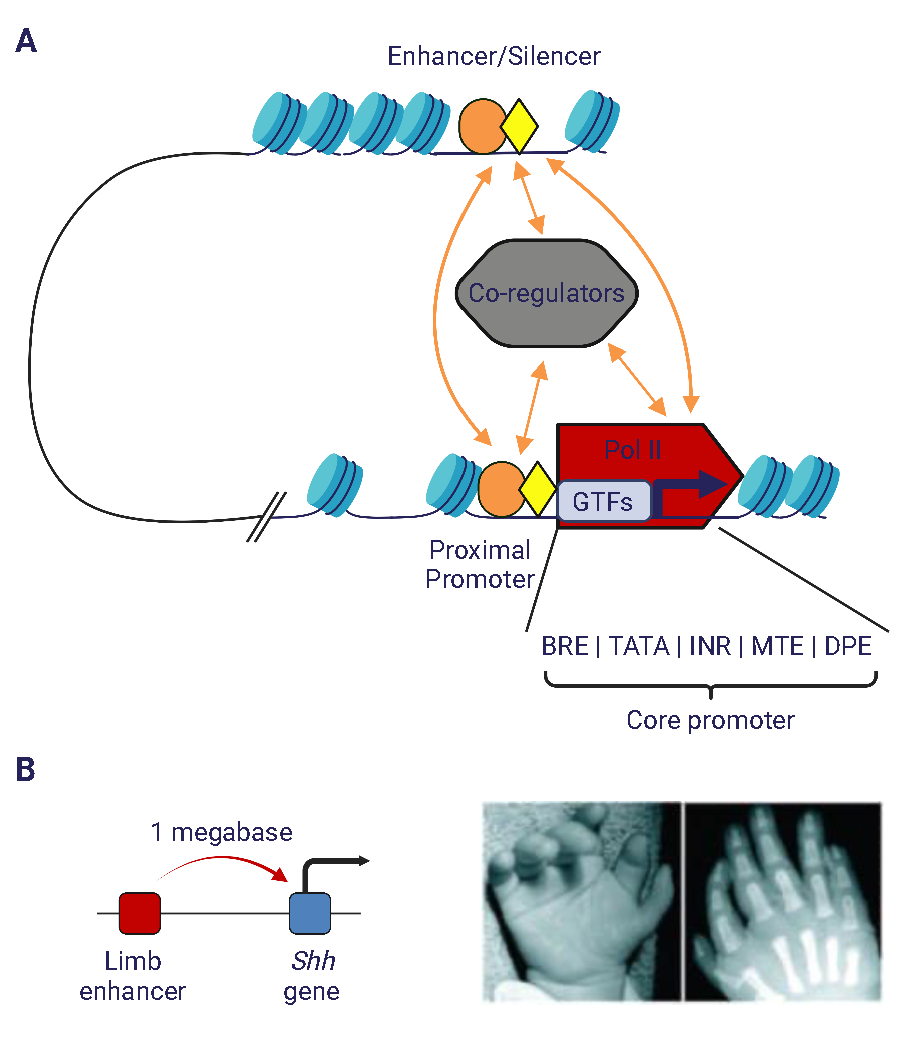
\includegraphics[width=0.8\textwidth]{chapter1/figures/fig1.pdf}
    \caption[\textit{Cis}-regulatory elements in the genome]{\textbf{\textit{Cis}-regulatory elements in the genome. (A)} Schematic view of \textit{cis}-regulatory elements around the core promoter, proximal promoter and enhancer/silencer regions. The \textit{cis}-regulatory elements within the core promoter including BRE, TATA, INR, MTE and DPE elements are bound by the general transcription factors (GTFs, blue rectangle). Other responsive elements within the proximal promoter and enhancer/silencer regions are recognised by regulatory transcription factors (orange ovals and yellow diamonds). Co-regulators (grey hexagon) are indirectly associated with the \textit{cis}-regulatory elements by binding to the transcription factors. Transcription factors and co-regulators regulate the transcription mediated by the RNA polymerase II (Pol II, red rocket). Orange and black arrows indicate the protein-protein interaction and the transcription start site respectively. \textbf{(B) Left,} schematic view of the spatial-relationship between the limb enhancer and the \textit{Shh} gene. \textbf{Right,} an example of hands from the patient with a single point mutation in the \textit{Shh} gene limb enhancer region (adapted from \cite{fuda2009defining} and \cite{visel2009genomic}).}
    \label{fig:fig1}
\end{figure}

The genetic code is stored in the coding exons within the gene body, but the information that controls the spatial-temporal expression of a gene is encoded in the DNA sequences called \textit{cis}-regulatory elements. In general, the DNA sequences within these regions can target the assembly of transcription factor complexes, consequently activating or repressing the transcription of a gene. The \textit{cis}-regulatory element can be mainly categorised into three groups according to its distance relative to the transcription start site (TSS) of a gene: the core promoter, the proximal promoter, and the enhancer/silencer (reviewed in \cite{visel2009genomic}). The core promoter is mostly located within tens of base pairs of a TSS. Common core promoter elements include the TATA box (TATA), the TFII\underline{B} \underline{r}ecognition \underline{e}lement (BRE), the \underline{in}itiato\underline{r} element (INR), the \underline{m}otif \underline{t}en \underline{e}lement (MTE), and the \underline{d}ownstream \underline{p}romoter \underline{e}lement (DPE). These elements can be bound by the general transcription factors which help recruit the \underline{p}re-\underline{i}nitiation \underline{c}omplex (PIC) and subsequently specify the TSS (reviewed in \cite{juven-gershon2008the}). The proximal promoter is close, usually upstream, to the core promoter, and the enhancers/silencers are generally located at distal regions from the TSS. The promoter and enhancer/silencer contain DNA sequences called \underline{r}esponsive \underline{e}lements (REs) which can be recognised by sequence-specific binding transcription factors. They help recruit transcription activators/repressors and consequently change the transcription of the downstream genes (\textbf{Figure \ref{fig:fig1}A})(reviewed in \cite{fuda2009defining}).

Besides the recruitment of transcription factors by pure DNA sequences, the nucleotides within the \textit{cis}-regulatory element also undergo modifications which often affect gene transcription. For example, the cytosines in the CpG sites in mammals tend to be methylated to 5-methylcytosine (5mC) which is usually associated with mutation (5mc $\rightarrow$ T) and gene silencing (reviewed in \cite{deaton2011cpg}). In addition, recent studies have shown that enzymes from the Tet family can catalyse the conversion of 5mC to 5hmC which is prevalent in mammalian cells, especially in neuronal cells of the central nervous system (\cite{kriaucionis2009the,tahiliani2009conversion}).

Though they do not directly encode proteins, the \textit{cis}-regulatory elements are equally important as the protein-coding sequences. This can be demonstrated by the discovery that a single nucleotide mutation within the limb enhancer, which is located at 1 megabase away from the \textit{Shh} gene and does not encode any proteins, severely disturbs the proper limb formation in mouse and human (\textbf{Figure \ref{fig:fig1}B}) (\cite{lettice2003a,sagai2005elimination}). Recent genomic studies strongly suggest variations in \textit{cis}-regulatory elements in gene expression (reviewed in \cite{visel2009genomic}).

\subsection{Transcription factors} \label{section:tf}

Transcription factors can decipher the code held within the \textit{cis}-regulatory element by directly binding to their responsive elements to regulate gene transcription. Generally, transcription factors can be divided into two distinct groups (\cite{lemon2000orchestrated}):

\textbf{(1) General transcription factors (GTFs):} \underline{G}eneral \underline{t}ranscription \underline{f}actors (GTFs) include TFIIA, TFIIB, TFIID, TFIIE, TFIIF, and TFIIH (reviewed in \cite{reese2003basal,thomas2006the,sikorski2009the}). Together with Pol II, GTFs bind to the aforementioned cis-regulatory elements within the core promoter regions to form the PIC, which is a significant event in transcription initiation (reviewed in \cite{juven-gershon2008the}).

\textbf{(2) Regulatory transcription factors:} Regulatory transcription factors can recognise and bind to specific DNA sequences, \textit{i.e.} their responsive elements, within the proximal promoter or enhancer/silencer regions by their \underline{D}NA-\underline{b}inding \underline{d}omain (DBD) to either activate (activators) or repress (repressors) transcription. These factors usually facilitate the formation and the stabilisation of the PIC, or help the recruitment of required co-regulators and chromatin-modifying factors, which results in a change of the gene transcription (reviewed in \cite{ptashne1988how,narlikar2002cooperation}). In this study and most research papers, the term \enquote{transcription factor} generally refers to this kind of transcription factors. Usually, transcription factors are classified according to their DBDs. Among them are the well-known domains: helix-turn-helix (\textit{e.g.}, homeobox), helix-loop-helix (\textit{e.g.}, MyoD and Myogenin), zinc finger (\textit{e.g.}, SP1), basic leucine zipper (\textit{e.g.}, c-Jun and c-Fos) (reviewed in \cite{latchman1997transcription}).

In addition to DNA-binding transcription factors, other proteins like co-regulators and chromatin-modifying factors which do not directly contact DNA are also important for the transcriptional regulation of a gene. Co-regulators generally provide additional connections between regulatory transcription factors and the GTFs or Pol II through protein-protein interactions, leading to the activation or repression of the gene (reviewed in \cite{näär2001transcriptional}).

Chromatin-modifying factors contain two kinds of complex: (1) chromatin remodellers, enzymes that reposition, reconfigure or eject nucleosomes in a noncovalent manner using the energy from ATP hydrolysis (reviewed in \cite{cairns2009the,becker2002atp-dependent}), and (2) chromatin modifiers, enzymes that covalently modify nucleosomes (\cite{cairns2009the,narlikar2002cooperation}).

Chromatin remodellers are able to disrupt the interaction between the DNA and the core histone surface, which results in either a displacement or a shift of histone octamers to adjacent positions (reviewed in \cite{narlikar2002cooperation}). Chromatin modifiers covalently change nucleosomes by modifications of histone tails such as acetylation, methylation, phosphorylation, ubiquitination, and sumoylation (reviewed in \cite{narlikar2002cooperation,bannister2005reversing,shilatifard2006chromatin}). These modifications not only alter the electrostatic DNA-histone interaction, but also provide docking sites for the recruitment of non-histone regulatory proteins and the transcription machinery, subsequently leading to transcription activation or repression.

\subsection{Transcription stages}

Transcription is a multistage process, which consists of at least six major steps (\textbf{Figure \ref{fig:fig2}}): chromatin remodelling, initiation, Pol II pausing, elongation, termination, and re-initiation (reviewed in \cite{fuda2009defining}).

\begin{figure}[!ht]
    \centering
    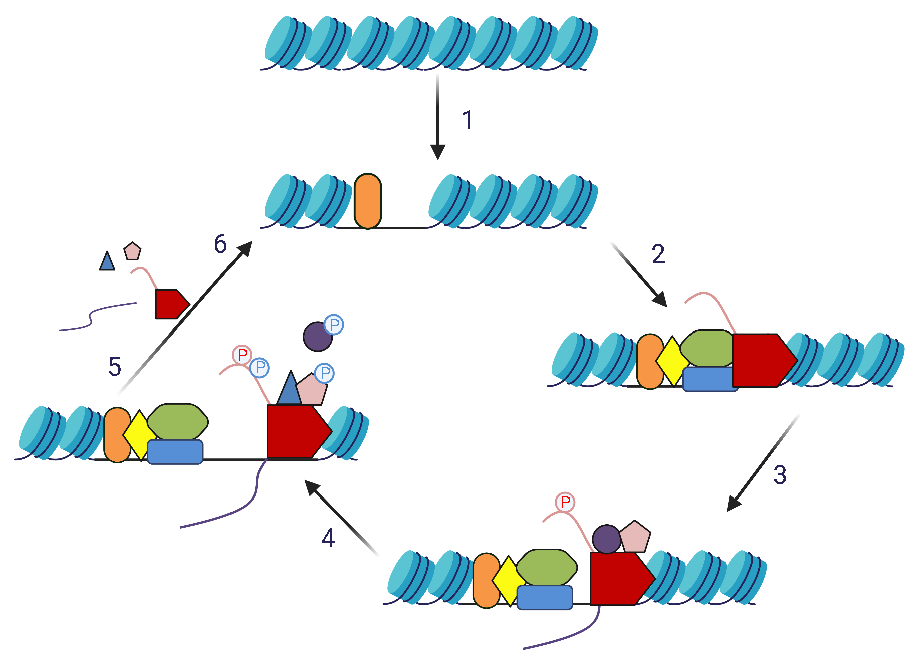
\includegraphics[width=0.9\textwidth]{chapter1/figures/fig2.pdf}
    \caption[Different stages of transcription]{\textbf{Different stages of transcription. Stage 1:} chromatin remodelling. The gene and its regulatory regions are packaged as nucleosomes (light brown). An activator (orange ovals) binds to DNA and recruits chromatin remodelling complex to make the promoter open for transcription factor binding. \textbf{Stage 2:} initiation. A second activator (yellow diamond) binds, promotes the binding of GTFs (blue rectangles) and recruits co-activators (green hexagons), facilitating Pol II (red rocket) entry to the PIC. Consequently, DNA is unwound at the TSS, and an open complex is formed. \textbf{Stage 3:} Pol II pausing. Pol II breaks contacts with promoter-bound factors, transcribes 20 - 50 bases downstream of the TSS, produces an RNA (purple lines) and pauses, which is mediated by DSIF (pink pentagon) and NELF complex (purple circle). The Ser residues at position 5 (Ser 5) of the Pol II carboxyl-terminal domain (CTD) repeats are phosphorylated (red Ps) during this stage. \textbf{Stage 4:} elongation. P-TEFb (blue triangles) is recruited directly or indirectly by the activator and phosphorylates Ser 2 of the Pol II CTD repeats, DSIF and the NELF subunits (blue Ps). NELF dissociates from the rest of the complex. Pol II escapes from the pause, travelling along the gene body. Productive elongation happens. \textbf{Stage 5:} termination. After the Pol II complex transcribes the gene, it is removed from the DNA, and the RNA is released. \textbf{Stage 6:} re-initiation. The freed Pol II can re-initiate (adapted from \cite{fuda2009defining})}
    \label{fig:fig2}
\end{figure}

\subsubsection{Stage 1: Chromatin remodelling}

In eukaryotes, the DNA is wrapped around histone octamers to form nucleosomes, the fundamental units of eukaryotic chromatin (\cite{kornberg1974chromatin}). Although this kind of DNA wrapping compacts the genome, it also prevents transcription initiation by restricting the DNA-binding events of transcription factors (reviewed in \cite{cairns2009the}). Therefore, the occurrence of transcription requires changes of chromatin structure by chromatin- modifying factors, so that transcription factors and Pol II can gain access to the promoter of a gene (\cite{boeger2003nucleosomes}).

\subsubsection{Stage 2: Transcription initiation}

The second stage of transcription is initiation, the most extensively-studied event during the process of transcription. Transcription initiation begins with the formation of PIC (reviewed in \cite{martinez2002multi-protein}). At the start of PIC formation, TFIID binds to the core promoter elements, followed by TFIIB binding to the promoter. Together, they recruit other GTFs and Pol II through either a sequential assembly or a preassembled Pol II holoenzyme pathway (reviewed in \cite{thomas2006the}). \textit{In vitro} studies show that the PIC is sufficient for basal levels of transcription (\cite{reese2003basal,thomas2006the}). However, this complex does not respond to activators and cannot start transcription of chromatin templates \textit{in vivo} (reviewed in \cite{sikorski2009the}). Therefore, a multitude of co-regulators and chromatin-modifying factors are also needed in the promoter region of the gene. For example, Mediators can bind to the carboxyl terminal domain (CTD) of Pol II, connecting Pol II and other transcription factors, which is required for most Pol II mediated transcription (reviewed in \cite{björklund2005the}). The regulatory transcription factors, the co-regulators, the chromatin-modifying factors, together with the PIC and gene promoters, are connected with each other, forming a transcription initiation complex through protein-protein and protein-DNA interactions. After formation of this initiation complex, transcription will enter into the next stage.

\subsubsection{Stages 3-6: Pol II pausing, elongation, termination, and re-initiation}

It was once believed that transcription was rarely regulated during the stages after the initiation. However, some early studies at the gene-specific level demonstrated that certain genes, such as the \textit{Drosophila Hsp70} gene, experience transcription initiation but show no productive elongation, \textit{i.e.} the Pol II is paused at the promoter regions (\cite{rougvie1988the}). This is the first clue of the existence of post-initiation regulatory stages. Recent genome-wide studies suggest the Pol II pausing is prevalent and important for metazoan protein-coding genes, especially those that are involved in stimulus-responsive gene networks (\cite{guenther2007a,gilchrist2012regulating}). After the transcription initiation, the pausing factors \underline{ne}gative \underline{el}ongation \underline{f}actor (NELF) and \underline{D}RB-\underline{s}ensitivity \underline{i}nducing \underline{f}actor (DSIF) generate a paused Pol II just downstream of the TSS (\cite{yamagata2008arginine}). The release of the paused Pol II to productive elongation requires the recruitment of the \underline{p}ositive \underline{t}ranscription \underline{e}longation \underline{f}actor \underline{b} (P-TEFb) to the paused Pol II, which subsequently phosphorylates the components in the initiation complex, including Pol II, NELF, and DSIF (\cite{core2008transcription}). A more recent study shows that the transcription factor c-Myc recruits P-TEFb to help the escape of paused Pol II (\cite{rahl2010c-myc}). Once escaped from the pausing, productive elongation will occur. Transcription termination and re-initiation are the least characterised stages.

In this study, we only concentrate on the first two stages of transcription: chromatin remodelling and initiation.

\section{The cell cycle regulation}

\subsection{General characteristics of the cell cycle events}

The cell cycle is the sequence of highly regulated processes during which cells make exact replicas of themselves. The smooth progression of the cell cycle requires cyclic expressions of certain genes: they must be activated and only be activated at specific phases. Failure of activation or repression at the proper time often results in abnormal cell cycle events. The series of highly dynamic events during the cell cycle provide a perfect model for the study of the transcriptional regulation. In addition, since the cell cycle is a very basic and prevalent biological process, many cell cycle regulators and events are evolutionarily conserved.

The eukaryotic cell cycle is conventionally divided into four distinct phases: the DNA synthesis phase (S phase), the segregation of duplicated chromosomes during mitosis (M phase), and two gaps, one before (G1 phase) and one after (G2 phase) S phase (\textbf{Figure \ref{fig:fig3}A}). When cells are exposed to extracellular conditions that arrest cell proliferation, such as serum starvation which is a common method in laboratories to synchronise cells, they can leave the cell cycle and enter a quiescent state termed G0 phase, where they can remain for days, weeks or even years before re-entering the cell cycle (reviewed in \cite{62}).

\begin{figure}[!ht]
    \centering
    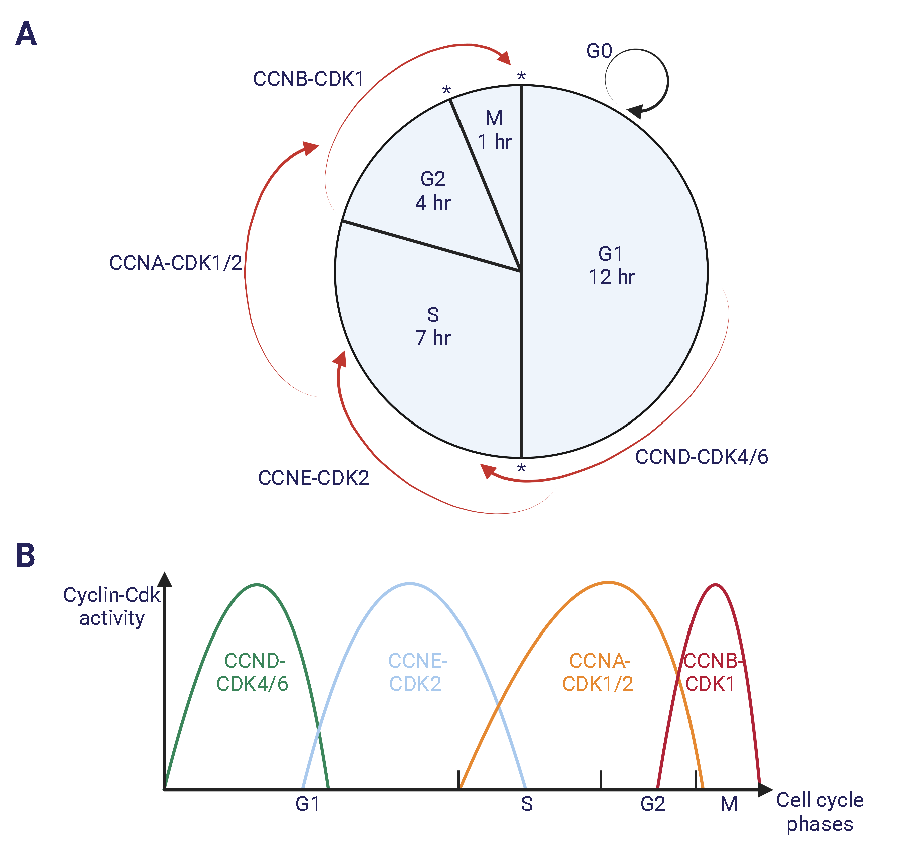
\includegraphics[width=0.8\textwidth]{chapter1/figures/fig3.pdf}
    \caption[The classical and minimal models of the cell-cycle control]{\textbf{The classical and minimal models of the cell-cycle control. (A)} Schematic view of the regulation of cell cycle progression by the relay of different Cyclin-Cdk complexes. Checkpoints (*) and the duration of each phase of a typical mammalian cell cycle are indicated. \textbf{(B)} Simplified view of activities of various Cyclin-Cdk complexes at different phases of the cell cycle (adapted from \cite{hochegger2008cyclin-dependent}).}
    \label{fig:fig3}
\end{figure}

The progression of the cell cycle requires at least three transitions, also called checkpoints, at the onset of S phase and at entry and exit of mitosis. All key stages in the cell cycle are subjected to these transitions, at which cells will \enquote{check} whether earlier processes, such as DNA replication and chromosome segregation, have been properly completed. Cells have the option to arrest the cell cycle if something goes wrong, preventing \enquote{abnormal} cells from proceeding to the next stage. At the heart of these switch-like transitions are the \underline{c}yclin-\underline{d}ependent \underline{k}inases (CDKs) and their regulatory subunits termed cyclins (reviewed in \cite{nurse2000a,hochegger2008cyclin-dependent}).

The CDKs, which have been described as a \enquote{cell cycle engine}, are serine/threonine protein kinases that drive cells through the cell cycle (reviewed in \cite{ds}). They are generally inactive without their cyclin partners. In most cases, the levels of CDKs are relatively constant throughout the cell cycle, whereas the concentration of most cyclins oscillates. Each CDK is activated by binding to its relevant cyclin during specific phases of the cell cycle, and in turn promotes phosphorylation of target substrates required for cell cycle progression. Therefore, progression through the various phases of the cell cycle is coordinated by waves of activation of CDKs. According to the traditional view once the cell enters into G1 phase after receiving appropriate signals, cyclin D (CCND)- CDK4/6 complexes are required during the progression of G1; at the G1/S checkpoint, CCNE-CDK2 complex is needed to start S phase; then CCNA-CDK1/2 complexes are responsible for the execution of S phase; at G2/M checkpoint, the CCNB-CDK1 complex is indispensable for the entry and progression of mitosis (\textbf{Figure \ref{fig:fig3}B}). However, this model has been challenged by recent studies indicating that mice that lack CDK2 are viable and healthy (\cite{ortega2003cyclin-dependent,berthet2003cdk2}). A more recent study uses mouse embryos lacking all CDKs that are thought to be essential in interphase (CDK2, CDK3, CDK4 and CDK6) and reveals that CDK1 is sufficient to drive all the events during the cell cycle. In this situation, CDK1 bound to all cyclins, leading to the proceeding of cellular events, such as phosphorylation of retinoblastoma protein pRb, which is required for S phase entry (\cite{santamaría2007cdk1}). Studies of \textit{Cdk} knock-out mice have shown us that deletion of \textit{Cdk1} is lethal (\cite{santamaría2007cdk1}). In addition, deletion of other \textit{Cdks} in mice results in some functional deficiencies, such as sterility (\textit{Cdk2}) (\cite{ortega2003cyclin-dependent,berthet2003cdk2}) and lack of adult pancreatic $\beta$-cells and pituitary lactotrophs (\textit{Cdk4}) (\cite{rane1999loss}), but these mice are viable and even healthy. These studies inform us that only CDK1 is essential for the cell survival, while other CDKs are also needed to maintain normal functions of the cell. It has become clear that there are many other complex events driving the cell cycle, besides the sequential activation of various CDKs.

\subsection{Transcriptional regulation of mammalian G2-M genes}

As mentioned above, the cyclic expression of cell cycle genes is critical for the smooth progression of the cell cycle. Genes that are required for G2 and M progression must be kept inactive during G0 or G1 phase and turned on at the proper time during G2 and M phase. In mammals, this temporal expression is controlled by the DNA elements called the CDE (\underline{c}ell cycle-\underline{d}ependent \underline{e}lement) and the CHR (\underline{c}ell cycle genes \underline{h}omology \underline{r}egion) within their promoters. In addition, the CCAAT-box element which is bound by the transcription factor NF-Y is also present in most cell cycle genes, though not restricted to G2-M genes, and is required for the activation of the gene (reviewed in \cite{müller2010the}). The CDE is a 6 base pair long GC-rich sequence, and a typical CHR consensus is TTTRAA where R represents an A or G (reviewed in \cite{müller2010the}). Early studies suggest that the CDE and the CHR elements are important for keeping the G2-M genes repressed during G0 and G1 phases, as mutations of these two elements in quiescent cells result in the hyperactivation of G2-M genes in resting cells (\cite{lucibello1995periodic,tommasi1995in,zwicker1995cell}). A most recent study demonstrates that the CHR element is absolutely required for both the repression and the activation of the G2-M genes, but the CDE element is not always present in the promoters (\cite{müller2012the}). Mutation of the CDE element has marginal effects on gene expression in most cases, but disruption of the CHR element unanimously gives rise to deregulation of the G2-M genes, leading to a derepression during G0 and a failure of activation in G2 and M phases (\cite{müller2012the}). Indeed, sequence alignment across different species of promoters from typical genes whose expression peak at the G2 and M phases shows that only the CHR and the CCAAT-box, not the CDE element, is evolutionarily conserved (\textbf{Figure \ref{fig:fig4}A}) (reviewed in \cite{müller2010the}).

A lot of CDE/CHR containing genes are negatively regulated by the tumour suppressor p53 (reviewed in \cite{müller2010the}). In many cases, the p53-dependent repression is, in part, through the CDE/CHR elements, though these elements are not directly bound by p53 (reviewed in \cite{müller2010the}). Only recently has an evolutionarily conserved multi-subunit protein complex been revealed to regulate the cell cycle gene expression through the CHR element. In G0 phase, the transcription factors DP and E2F4, together with RBL2 (a.k.a p130) and homologs of the \textit{C. elegans} synthetic \underline{mu}lti\underline{v}ulva class \underline{B} (MuvB) including LIN9, LIN37, LIN52, LIN54, and LIN53/RBBP4, are associated together to form a complex, namely DREAM, sitting on the promoters of most cell cycle genes to keep them repressed. When cells enter the cell cycle, the DREAM complex dissociates from the promoters of the cell cycle genes, resulting in the loss of repression of the genes that are required for the cell cycle. In the meantime, MuvB is separated from DP, E2F4 and RBL2 and interacts with another transcription factor B-MYB (a.k.a MYBL2), forming a new complex called MMB. In G2 and M phases, the MMB complex binds to the promoters of many genes that are required for the G2-M transition (but not genes that are required for G1-S transition) to activate their expression (\cite{litovchick2007evolutionarily,müller2012the,sadasivam2012the}). Importantly, the binding of the DREAM/MMB complexes to the DNA requires an intact CHR element in the promoter of the G2-M gene (\cite{müller2012the}) (\textbf{Figure \ref{fig:fig4}B}).

\begin{figure}[!t]
    \centering
    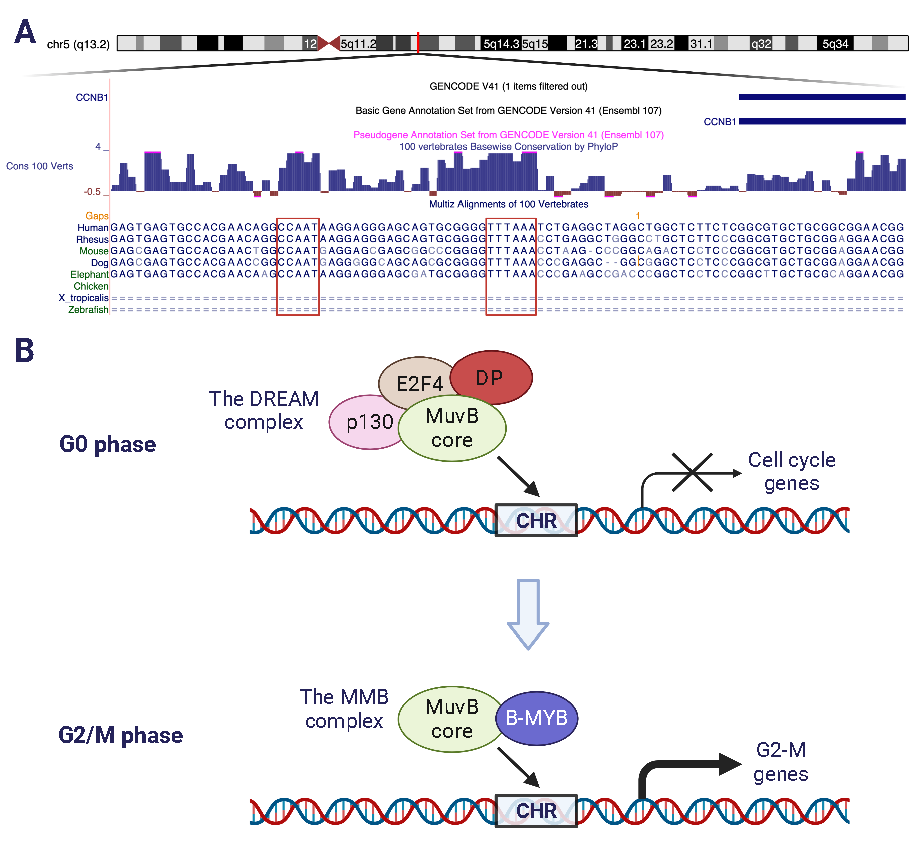
\includegraphics[width=0.8\textwidth]{chapter1/figures/fig4.pdf}
    \caption[The CHR element and the DREAM/MMB complex are important for the regulation of G2-M transition]{\textbf{The CHR element and the DREAM/MMB complex are important for the regulation of G2-M transition. (A)} Sequence alignment of the promoter of \textit{CCNB1}, a typical gene that is required for the G2-M transition, across different species. Two highly conserved elements the CCAAT-box and the CHR motifs are highlighted. \textbf{(B)} Schematic and simplified view of the regulation of the cell cycle by the DREAM/MMB complexes. In G0 phase, the MuvB core interacts with E2F4, DP1, and p130 (the DREAM complex) to keep the cell cycle genes repressed. This repression is mediated by the CHR motif. When cells enter the cell cycle, the DREAM complex dissociates from the promoters and disassembles, resulting in derepression of the cell cycle genes. In G2 and M phases, the MuvB core comes back to the promoter of genes that are required for G2-M transition (but not for G1-S transition) together with B-MYB (the MMB complex), leading to the activation of the genes. The activation is also mediated through the CHR motif.}
    \label{fig:fig4}
\end{figure}

Interestingly, the DREAM-like complex is also observed in flies and worms, though there are some differences in the components (\cite{Beall2002-mq,korenjak2004native}). Due to the lack of a B-MYB ortholog in worms, the MMB-like complex is only seen in mammals and flies (\cite{harrison2006some}). The roles of the CHR element and the DREAM/MMB complexes in cell cycle regulation were discovered separately, and have finally converged recently.

\section{Forkhead transcription factors}

\subsection{General characteristics of Forkhead transcription factors}

The defining feature of Forkhead transcription factors is the evolutionarily conserved DNA-binding domain: the Forkhead box (FOX) domain, which contains approximately 110 amino acid residues. The first discovered member of Forkhead transcription factor family was the region-specific homeotic gene \textit{forkh head (fkh)}. Mutation of this gene caused spiked-head structures in embryos of the \textit{Drosophila}, hence the name fork head (\cite{weigel1989the}). Over 100 genes encoding Forkhead proteins were later detected in various species ranging from yeast to human (reviewed in \cite{lai1993hepatocyte,kaufmann1996five}). X-ray crystallographic analysis and NMR spectroscopic analysis have shown that the canonical Forkhead box resembles a \enquote{winged helix} structure, which contains three $\alpha$-helices, three $\beta$-sheets and two loops or wings, typically arranged in an order of \enquote{$\alpha 1 - \beta 1 - \alpha 2 - \alpha 3 - \beta 2 - W1 - \beta 3 - W2 $} (see \textbf{Chapter \ref{ch:discussion}, Figure \ref{fig:fig53}}) (\cite{clark1993co-crystal,jin1999dynamic,van-dongen2000solution}). The primary binding interaction is through the third $\alpha$-helix ($\alpha 3$) which makes direct contacts with the target DNA in the major groove (\cite{clark1993co-crystal,marsden1998structural}).

It has been 20 years since the discovery of the first member of Forkhead transcription factor family. Hundreds of Fox genes have been identified from various species, and the number of Fox genes seems to rise with the increase of their anatomical complexity, from four in budding yeast to over forty in humans (reviewed in \cite{wijchers2006in,hannenhalli2009the}).

\subsection{Forkhead transcription factors and the cell cycle}

Forkhead (FOX) transcription factors are indispensable in regulating the expression of genes that are essential in a diverse range of biological processes, from cell cycle control to stress resistance, from language acquisition to appetite and body weight control. A subset of FOX proteins are key players in the cell cycle control, which have attracted a lot of attention.

\subsubsection{Fkh2p and the cell cycle control in budding yeast}

In yeast, the \textit{CLB2} gene cluster whose transcription level peaks at the G2 and M phase contains 33 genes, such as \textit{CLB1}, \textit{CLB2}, \textit{SWI5}, \textit{CDC5}, \textit{CDC20} and other genes which are critical for the events during mitosis (\cite{spellman1998comprehensive}). The transcription of genes within this cluster is controlled by a transcription factor complex that consists of the MADS-box transcription factor Mcm1p, the Forkhead transcription factor Fkh2p, and the coactivator Ndd1p (\cite{koranda2000forkhead-like,darieva2006polo}) (\textbf{Figure \ref{fig:fig5}}, top panel). The activity of this ternary complex is regulated through sequential phosphorylation of Fkh2p by the cyclin-cdk complex Clb5p-Cdc28p (\cite{pic-taylor2004regulation}), and Ndd1p by Clb2p- Cdc28p (\cite{darieva2003cell,reynolds2003recruitment}) and by Cdc5p (\cite{darieva2006polo}). Interestingly, Clb2p and Cdc5p themselves are also encoded by the genes within the \textit{CLB2}  cluster. Hence, this mode of transcription generates a positive feedback loop during the G2 and M phases, ensuring the smooth progression of the cell cycle at these stages (\textbf{Figure \ref{fig:fig5}}, top panel).

\subsubsection{FOXM1 and the cell cycle control}

Mammalian FOXM1 is a proliferation-specific transcription factor which exhibits cell cycle-dependent expression. Both FOXM1 mRNA and protein levels are barely detectable in quiescent cells and are at relatively low levels in G1 phase. The expression (both mRNA and protein) of FOXM1 begins to increase in S phase, peaks when cells enter G2 and M phases, and then decreases at the late M phase (\cite{ye1997hepatocyte,korver1998uncoupling,park2008anaphase-promoting}). There are three isoforms of human FOXM1 protein due to differential splicing of two alternative exons: FOXM1a, FOXM1b and FOXM1c. Both FOXM1b and FOXM1c are transcription activators, whereas FOXM1a does not transactivate because of an additional exon in the C-terminal transactivation domain (reviewed in \cite{laoukili2007foxm1:}). Until now, only FOXM1b and FOXM1c have been studied, which together are referred to as FOXM1 in the following section unless otherwise specified.

\begin{figure}[!t]
\centering
    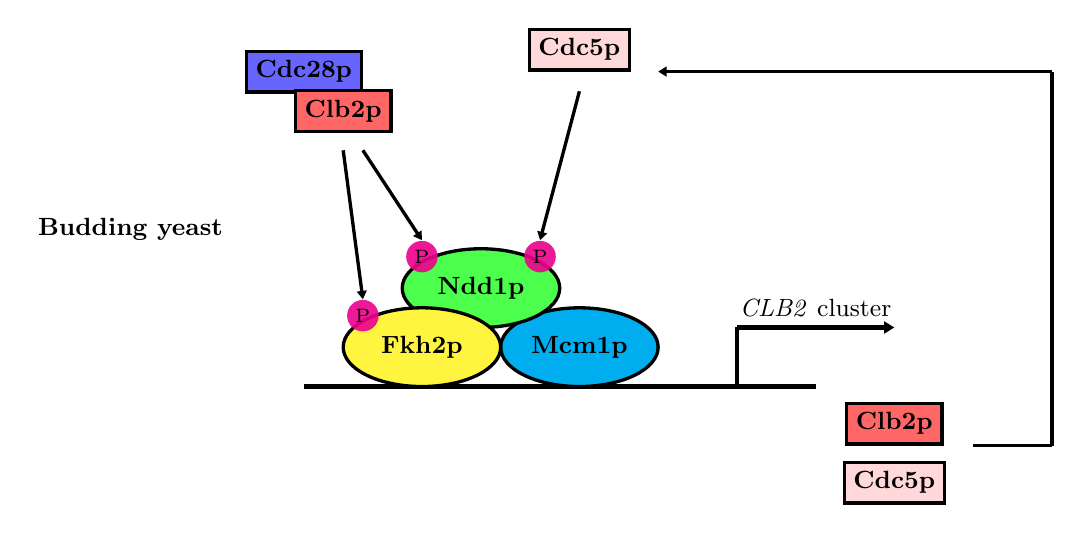
\begin{tikzpicture}
        \draw (0,3.5) node[anchor=west] {\small \textbf{Budding yeast}};
        \draw (11,0) node[draw, very thick, anchor=south, fill=pink!60] {\small \textbf{Cdc5p}};
        \draw (11,0.75) node[draw, very thick, anchor=south, fill=red!60] {\small \textbf{Clb2p}};
        \draw[ultra thick] (3.5,1.5) -- (10,1.5);
        \draw[ultra thick, ->, >={Triangle[scale=0.5]}] (9,1.5) -- (9,2.25) (9,2.25) -- (11,2.25) node[anchor=south, pos=0.5] {\small \textit{CLB2} cluster};
        \draw (7,5.5) node[draw, very thick, anchor=south, fill=pink!60] {\small \textbf{Cdc5p}}
              (3.5,5.5) node[draw, very thick, fill=blue!60] {\small \textbf{Cdc28p}}
              (4,5) node[draw, very thick, fill=red!60] {\small \textbf{Clb2p}};
        \draw[very thick, fill=cyan] (7,2) circle[x radius=1, y radius=0.5];
        \draw[very thick, fill=green!70] (5.75,2.75) circle[x radius=1, y radius=0.5];
        \draw[very thick, fill=yellow!75] (5,2) circle[x radius=1, y radius=0.5];
        \draw[draw=none, fill=magenta, opacity=0.9] (4.25,2.4) circle[radius=0.2]
             (5,3.15) circle[radius=0.2] (6.5,3.15) circle[radius=0.2];
        \draw (7,2) node {\small \textbf{Mcm1p}} (5,2) node {\small \textbf{Fkh2p}} (5.75,2.75) node {\small \textbf{Ndd1p}} (4.25,2.4) node (p1) {\scriptsize P} (5,3.15) node (p2) {\scriptsize P} (6.5,3.15) node (p3) {\scriptsize P};
        \draw[->, very thick, >={Triangle[scale=0.5]}] (4,4.5) -- (p1.north);
        \draw[->, very thick, >={Triangle[scale=0.5]}] (4.25,4.5) -- (p2.north);
        \draw[->, very thick, >={Triangle[scale=0.5]}] (7,5.25) -- (p3.north);
        \draw[->, very thick, >={Triangle[scale=0.5]}] (12,0.75) -- (13,0.75) (13,0.75) -- (13,5.5) (13,5.5) -- (8,5.5);
    \end{tikzpicture}
    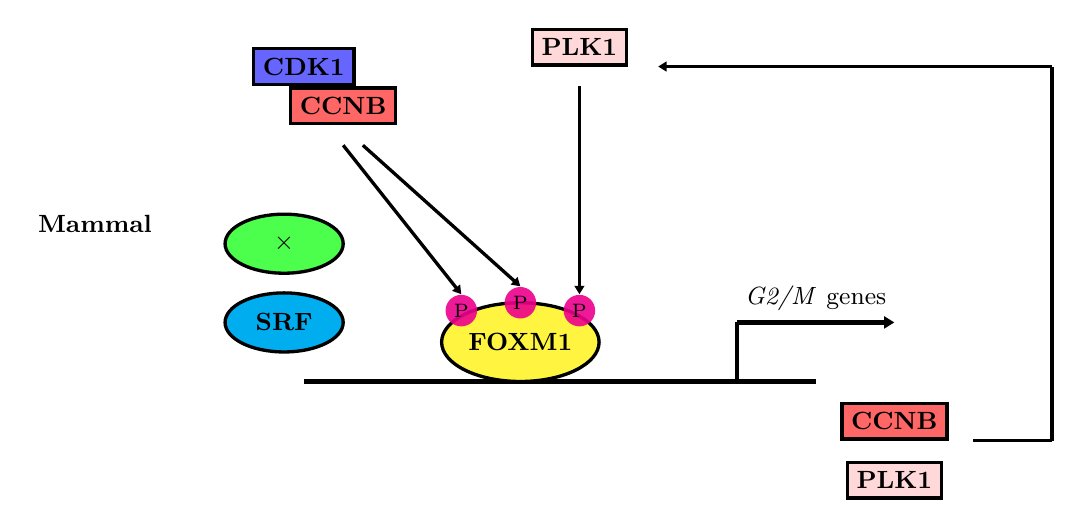
\begin{tikzpicture}
        \draw (0,3.5) node[anchor=west] {\small \textbf{Mammal}};
        \draw (11,0) node[draw, very thick, anchor=south, fill=pink!60] {\small \textbf{PLK1}};
        \draw (11,0.75) node[draw, very thick, anchor=south, fill=red!60] {\small \textbf{CCNB}};
        \draw[ultra thick] (3.5,1.5) -- (10,1.5);
        \draw[ultra thick, ->, >={Triangle[scale=0.5]}] (9,1.5) -- (9,2.25) (9,2.25) -- (11,2.25) node[anchor=south, pos=0.5] {\small \textit{G2/M} genes};
        \draw (7,5.5) node[draw, very thick, anchor=south, fill=pink!60] {\small \textbf{PLK1}}
              (3.5,5.5) node[draw, very thick, fill=blue!60] {\small \textbf{CDK1}}
              (4,5) node[draw, very thick, fill=red!60] {\small \textbf{CCNB}};
        \draw[very thick, fill=cyan] (3.25,2.25) circle[x radius=0.75, y radius=0.375];
        \draw[very thick, fill=green!70] (3.25,3.25) circle[x radius=0.75, y radius=0.375];
        \draw[very thick, fill=yellow!75] (6.25,2) circle[x radius=1, y radius=0.5];
        \draw[draw=none, fill=magenta, opacity=0.9] (5.5,2.4) circle[radius=0.2]
             (6.25,2.5) circle[radius=0.2] (7,2.4) circle[radius=0.2];
        \draw (3.25,2.25) node {\small \textbf{SRF}} (6.25,2) node {\small \textbf{FOXM1}} (3.25,3.25) node {\small $\times$} (5.5,2.4) node (p1) {\scriptsize P} (6.25,2.5) node (p2) {\scriptsize P} (7,2.4) node (p3) {\scriptsize P};
        \draw[->, very thick, >={Triangle[scale=0.5]}] (4,4.5) -- (p1.north);
        \draw[->, very thick, >={Triangle[scale=0.5]}] (4.25,4.5) -- (p2.north);
        \draw[->, very thick, >={Triangle[scale=0.5]}] (7,5.25) -- (p3.north);
        \draw[->, very thick, >={Triangle[scale=0.5]}] (12,0.75) -- (13,0.75) (13,0.75) -- (13,5.5) (13,5.5) -- (8,5.5);
    \end{tikzpicture}
    \caption[Transcription programs that regulate the G2-M transition of yeast and human cell cycles]{\textbf{Transcription programs that regulate the G2-M transition of yeast and human cell cycles. Top,} schematic view of the positive feedback loop between the Mcm1p-Fkh2p-Ndd1p ternary complex and the proteins encoded by the CLB2 cluster in budding yeast. \textbf{Bottom,} schematic view of the positive feedback loop between FOXM1 and proteins that are required for the mitosis in mammals. The homologous proteins are drawn in matching colours, and the phosphorylation events are indicated by black arrows and pink Ps.}
    \label{fig:fig5}
\end{figure}

Many recent studies point out that FOXM1 is a master regulator of the G2 and M phase progression of the cell cycle. Knockdown of FOXM1 causes polyploidy and a delay in G2 (\cite{laoukili2005foxm1}). Both the depletion and the overexpression of FOXM1 induce the deregulation of a large array of genes that are required for the G2 phase and mitosis, and the yeast homologs of many FOXM1 target genes are within the \textit{CLB2} cluster (\cite{laoukili2005foxm1,wonsey2005loss,lefebvre2010a}). Like the ternary complex Mcm1p-Fkh2p-Ndd1p, the transcriptional activity of FOXM1 is also regulated by sequential phosphorylation by Cyclin-Cdk kinase complexes CCNA-CDK1/2, CCNB- CDK1 and by PLK1 (\cite{wang2005forkhead,fu2008plk1-dependent,laoukili2008activation}). Very intriguingly, CDK1, CCNB, and PLK1 are the mammalian orthologs of yeast Cdc28p, Clb2/5p, and Cdc5p respectively. Furthermore, \textit{CDK1}, \textit{CCNB}, and \textit{PLK1} are also FOXM1 target genes (\cite{laoukili2005foxm1,wang2005forkhead}). Clearly, a similar positive feedback loop also exists in mammalian cells to secure the progression of the G2 phase and mitosis (\textbf{Figure \ref{fig:fig5}}, bottom panel), although some differences are apparent: no evidence so far suggests that SRF, the mammalian MADS-box transcription factor, interacts with FOXM1 or the promoters of genes expressed in late G2 and M phases, and there is no Ndd1p ortholog in mammals or any other organisms (reviewed in \cite{murakami2010regulation}). It seems that FOXM1 is comparatively similar to the yeast Fkh2p, though they do not share any apparent homology at regions outside the Forkhead domain.

The positive feedback loop during the G2 phase and mitosis, mediated by Mcm1p- Fkh2p-Ndd1p in yeasts, and by FOXM1 in mammals, emphasises the importance of the Forkhead transcription factors in cell cycle control. In addition, the conservation of the components within the positive feedback loop also provides a good model for evolutionary studies.

\subsubsection{FOXOs and cell cycle control}

Another important set of regulators in the cell cycle control are the FOXO subfamily of Forkhead transcription factors, which share high sequence homology to the \textit{Caenorhabditis elegans} Forkhead transcription factor DAF-16 (reviewed in \cite{myatt2007the}). Actually, one of the first functions discovered for FOXOs was that they could regulate the G1/S transition (\cite{medema2000afx-like}). Currently, four FOXO isoforms have been identified in mammalian cells: FOXO1, FOXO3, FOXO4 and FOXO6. The expression of \textit{FOXO6} is limited to brain, thymus and kidney, whereas \textit{FOXO1}, \textit{FOXO3} and \textit{FOXO4} are ubiquitously expressed (reviewed in \cite{greer2005foxo}). Of note, in mammals, there are two \textit{FOXO3} genes, \textit{FOXO3a} and \textit{FOXO3b}, but \textit{FOXO3b} turns out to be a pseudogene (\cite{greer2005foxo}). The terms \textit{FOXO3A} and \textit{FKHRL1} are the most commonly-used names for the \textit{FOXO3} gene, but according to the HGNC (HUGO Gene Nomenclature Committee), the latest official gene symbol of this gene is \enquote{FOXO3} (\url{https://www.genenames.org/data/hgnc_data.php?hgnc_id=3821}). Therefore, \enquote{FOXO3} is used in this study. FOXO proteins have long been shown to play important roles in cell cycle arrest. Like other transcription factors, the transcriptional activities of FOXOs are extensively regulated by post-translational modifications like phosphorylation, methylation and acetylation (\cite{brunet1999akt,matsuzaki2005acetylation,yamagata2008arginine}). Phosphorylation is the most extensively-studied modification of the FOXO proteins.

Unlike Fkh2p and FOXM1, the phosphorylation of FOXOs mostly results in the inhibition of their transcriptional activities (\cite{brunet1999akt}). The FOXO proteins are key direct targets of the phosphatidylinositol 3-kinase (PI3K)-AKT signalling pathway (\cite{brunet1999akt}). AKT phosphorylates FOXOs at three important regulatory sites (Thr32, Ser253, and Ser315 in FOXO3 protein) which are conserved from worms to mammals (reviewed in \cite{greer2005foxo}). This AKT-mediated phosphorylation induces the nuclear export of FOXOs by the 14-3-3 proteins, which serve as chaperone molecules to escort them out of the nucleus, leading to the loss of transcriptional activity of FOXOs (\cite{brunet1999akt,brunet200214-3-3}). Similarly to the positive feedback loop in promoting the G2 and M phase progression, this PI3K-AKT-FOXO signalling cascade is also evolutionarily conserved from worms to mammals (\textbf{Figure \ref{fig:fig6}}).

The importance of this PI3K-AKT-FOXO signalling is underlined by the highly activated PI3K-AKT in many tumours (reviewed in \cite{myatt2007the}). Thus, FOXO proteins usually appear to be transcriptionally inactive in cancer cells. When the PI3K-AKT is inhibited, FOXOs will lose phosphorylation and enter into nucleus to activate many genes including \textit{p21\sus{CIP}} (\cite{seoane2004integration}), \textit{p27\sus{KIP1}} (\cite{medema2000afx-like}), \textit{CCNG2} (\cite{martínez-gac2004control}), and \textit{GADD45A} (\cite{tran2002dna}), all of which promote cell cycle arrest. Other targets of FOXOs like \textit{p15\sus{INKb}} and \textit{p19\sus{INK4d}}, and \textit{p130} also induce the cell cycle arrest (\cite{katayama2008foxo,kops2002control}). In addition, forced activation of FOXO3 and FOXO4 causes a delay in mitotic entry in U2OS cells (\cite{laoukili2005foxm1}), presumably due to the activation of \textit{CCNG2} and \textit{GADD45A}. Therefore, it is clear that FOXOs are key players in the regulation of cell cycle arrest.

\begin{figure}[t]
    \centering
    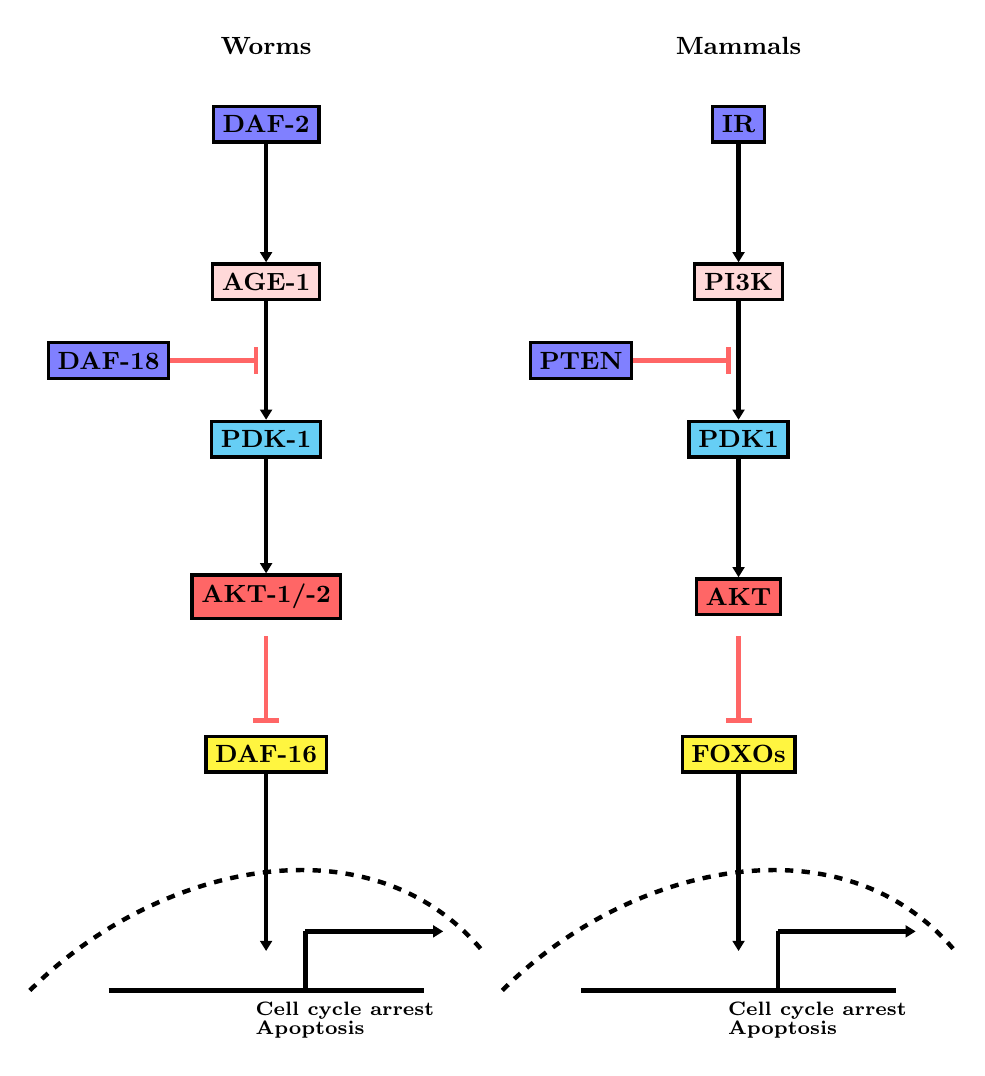
\begin{tikzpicture}[sqnode/.style={draw, very thick},
                        carrow/.style={->,ultra thick,>={Triangle[scale=0.5]}}]
        \draw (3,12) node {\small \textbf{Worms}} (9,12) node {\small \textbf{Mammals}};
        \draw (3,11) node[sqnode,fill=blue!50] (w1) {\small \textbf{DAF-2}}
              (9,11) node[sqnode,fill=blue!50] (m1) {\small \textbf{IR}}
              (3,9) node[sqnode,fill=pink!60] (w2) {\small \textbf{AGE-1}}
              (9,9) node[sqnode,fill=pink!60] (m2) {\small \textbf{PI3K}}
              (1,8) node[sqnode,fill=blue!50] (w3) {\small \textbf{DAF-18}}
              (7,8) node[sqnode,fill=blue!50] (m3) {\small \textbf{PTEN}}
              (3,7) node[sqnode,fill=cyan!60] (w4) {\small \textbf{PDK-1}}
              (9,7) node[sqnode,fill=cyan!60] (m4) {\small \textbf{PDK1}}
              (3,5) node[sqnode,fill=red!60] (w5) {\small \textbf{AKT-1/-2}}
              (9,5) node[sqnode,fill=red!60] (m5) {\small \textbf{AKT}}
              (3,3) node[sqnode,fill=yellow!75] (w6) {\small \textbf{DAF-16}}
              (9,3) node[sqnode,fill=yellow!75] (m6) {\small \textbf{FOXOs}};
        \draw[ultra thick] (1,0) -- (5,0) node[pos=0.75, anchor=north, align=left] {\scriptsize \textbf{Cell cycle arrest}\\[-5pt] \scriptsize \textbf{Apoptosis}}
                           (7,0) -- (11,0) node[pos=0.75, anchor=north, align=left] {\scriptsize \textbf{Cell cycle arrest}\\[-5pt] \scriptsize \textbf{Apoptosis}};
        \draw[carrow] (3.5,0)--(3.5,0.75) (3.5,0.75)--(5.25,0.75);
        \draw[carrow] (9.5,0)--(9.5,0.75) (9.5,0.75)--(11.25,0.75);
        \draw[ultra thick, dashed] (0,0) to[out=45, in=130] (5.75,0.5);
        \draw[ultra thick, dashed] (6,0) to[out=45, in=130] (11.75,0.5);
        \draw[carrow] (w1.south)--(w2.north);
        \draw[carrow] (w2.south)--(w4.north);
        \draw[carrow] (w4.south)--(w5.north);
        \draw[-|, ultra thick, red!60] (3,4.5)--(3,3.4);
        \draw[carrow] (w6.south)--(3,0.5);
        \draw[-|, ultra thick, red!60] (w3.east)--(2.9,8);
        \draw[carrow] (m1.south)--(m2.north);
        \draw[carrow] (m2.south)--(m4.north);
        \draw[carrow] (m4.south)--(m5.north);
        \draw[-|, ultra thick, red!60] (9,4.5)--(9,3.4);
        \draw[carrow] (m6.south)--(9,0.5);
        \draw[-|, ultra thick, red!60] (m3.east)--(8.9,8);
    \end{tikzpicture}
    \caption[Evolutionarily conserved PI3K/AKT/FOXOs pathway]{\textbf{Evolutionarily conserved PI3K/AKT/FOXOs pathway.} Schematic views of signalling cascade components of PI3K/AKT/FOXOs pathway in worms (left) and mammals (right). Phosphorylation events are indicated by black arrows, and inhibitory events are indicated by red lines. Homologous components in worms and mammals are drawn in matching colours.}
    \label{fig:fig6}
\end{figure}

However, one study demonstrates that FOXO3 can directly bind to the promoters of \textit{CCNB1} and \textit{PLK1}, to activate their transcription promoting G2 and M phase progression (\cite{alvarez2001forkhead}). This indicates an interesting possible functional redundancy of FOXO3 and FOXM1 in regulating the genes that are required for the G2 and M phases. However, a later study shows that activation of FOXO3 fails to rescue the mitotic defects of FOXM1-null cells, and is unable to reconstitute protein expression of CCNB1 and PLK1. Activation of endogenous FOXO3 by treatment with LY294002, a specific inhibitor of PI3K, in these FOXM1-null cells failed to induce \textit{PLK1} promoter activity (\cite{laoukili2005foxm1}). This evidence indicates that FOXO3 acts in a non-redundant fashion with FOXM1 in the G2 and M transition. On the other hand, another study demonstrates that, in mouse cells, CDK1 can phosphorylate FOXO1 at Ser249 which disrupts its interaction with the 14-3-3 protein, leading to the nuclear accumulation and occupancy of FOXO1 at the \textit{Plk} promoter during G2-M transition (\cite{yuan2008activation}). Whether FOXOs can promote cell cycle progression still needs further investigation.

\subsubsection{FOXKs and the cell cycle control}

In addition to the Forkhead domain, the yeast Forkhead transcription factor Fkh2p also contain another functional domain called the \underline{F}ork\underline{h}ead-\underline{a}ssociated domain (FHA). The FHA domain is critical for the cell cycle dependent expression of genes within the \textit{CLB2} cluster, because this domain is required for the recruitment of the co-activator Ndd1p (\cite{darieva2003cell}). In mammals, only FOXK proteins possess the FHA domain (reviewed in \cite{murakami2010regulation}). Therefore, based on sequence homology, the FOXK proteins seem to be the mammalian Fkh2p orthologs. This indicates that FOXK proteins may play similar roles of Fkh2p in the cell cycle control. Indeed, there are two FOXK proteins in human: FOXK1 and FOXK2, both of which are able to physically interact with the MADS-box transcription factors SRF in humans (\cite{freddie2007functional}). However, this FOXK-SRF complex does not have a direct connection to G2 and M phase cell cycle regulation. However, FOXK2 can be phosphorylated by cyclin-cdk complex and its protein level is regulated in a cell cycle dependent manner (\cite{freddie2007functional,marais2010cell}). Recent genome-wide studies demonstrate that only a small number of FOXK1 and FOXK2 target genes are involved in cell cycle regulation, and those gene are not extensively related to G2 and M phase progression, like homologs of the \textit{CLB2} gene cluster (\cite{grant2012live-cell,ji2012the}). In the FOXK1 case, some of its target genes are required for the G1/S transition, indicating it is important at this stage of the cell cycle (\cite{grant2012live-cell}).

Therefore, from a functional view, the FOXK proteins do not seem to be similar to the yeast Fkh2p, although they share high sequence homology. Their roles in cell cycle regulation still need further characterisation.

\subsubsection{Other Forkhead transcription factors and the cell cycle control}

Some evidence suggests other Forkhead transcription factors are also involved in the cell cycle regulation. For example, FOXA1 and BRCA1 can synergistically activate the transcription of \textit{p27\sus{KIP1}} (\cite{williamson2006brca1}); FOXG1 can prevent the activation of \textit{p21\sus{CIP1}} in response to the TGF$\beta$ signalling by blocking the FOXO-SMAD interaction (\cite{seoane2004integration}); a genome-wide study on FOXP3 shows that a subset of its target genes are important for the cell cycle regulation (\cite{katoh2011foxp3}); a most recent study suggests that knockdown of FOXA2, FOXJ3, FOXK1, and FOXL2 results in the impaired cell cycle oscillation of luciferase reporter driven by the \textit{E2F1} promoters and six tandem Forkhead consensus sequences (\cite{grant2012live-cell}).

Generally speaking, roles of these Forkhead transcription factors in the cell cycle regulation are not extensively studied, which is in contrast to FOXM1 and FOXOs.

\section{Transcription factor (TF)-DNA binding}

\subsection{Key factors in TF-DNA interactions \textit{in vivo}}

In a living cell, the TF-DNA binding events are highly dynamic and are controlled by various factors, such as the conformation of proteins and the shape of DNA (reviewed in \cite{garvie2001recognition,travers1989dna}). Here we mainly discuss the following aspects:

\textbf{(1) The chromatin status:} in eukaryotic cells, DNA is packaged into nucleosomes by histones, making DNA inaccessible to other proteins, such as transcription factors (reviewed in \cite{cairns2009the}). Fortunately, there are a lot of chromatin remodelling complexes to change the chromatin status (see \textbf{Section \ref{section:tf}}), leading to the disassembly of nucleosomes and making DNA accessible to proteins. Recent genome-wide research has observed that low nucleosome density is a common feature of yeast promoters (\cite{lee2004evidence,sekinger2005intrinsic}), and another study revealed that, in yeast, Pol II promoters contain a nucleosome depleted region located \textasciitilde 200 bp upstream of the start codon flanked on both sides by positioned nucleosomes (\cite{yuan2005genome-scale}). Later research found that similar nucleosome depleted regions also exist in the genome of higher organisms, such as \textit{Drosophila} and Humans (\cite{mavrich2008nucleosome,ozsolak2007high-throughput}). These nucleosome free regions are generally believed to be crucial in enhancing TF-DNA binding and facilitating subsequent transcription.

\textbf{(2) The sequence of DNA:} most TF-DNA binding is sequence-specific. It seems a protein could recognise its binding site by somehow \enquote{reading} the DNA sequence. This reading is believed to be achieved by the formation of a series of amino-acid- and base- specific hydrogen bonds between protein side chains and the edges of the DNA nucleotides that are exposed in the major groove and the minor groove (\cite{seeman1976sequence-specific,joshi2007functional,rohs2009the}). Although transcription factors have their own sequence preference, previous research has provided innumerable lines of evidence that a single sequence cannot fully explain all \textit{in vivo} binding of a certain transcription factor (\textit{e.g.} \cite{hollenhorst2009dna}). That is, a transcription factor can recognise and bind to several (\textit{i.e.} not one) specific DNA sequences. There are \textasciitilde 1400 transcription factors in humans according to a recent census of human transcription factors (\cite{vaquerizas2009a}). Though the consensus motifs for most families are known, systematic analyses of these \textasciitilde 1400 transcription factors have just started only recently (see \textbf{Section \ref{section:tech}}).

\textbf{(3) The cellular conditions:} the condition of a cell will fluctuate in response to stimuli, such as extracellular signals. These fluctuations might lead to changes of the transcription factor, e.g. the concentration, the post-translational modifications, the binding partners, or the subcellular localization of the transcription factor. All those changes will influence the TF-DNA binding events inside the cell. Several nuclear receptors provide perfect examples. Nuclear receptors, like ER, AR, and GR, are generally sequestered in the cytoplasm, rendering them unable to bind to DNA. After the proper stimuli, like ligand binding, they can enter into the nucleus and bind to their responsive elements (reviewed in \cite{olefsky2001nuclear}).

\subsection{Current question: how do transcription factors select their specific DNA binding sites in the genome?}

In order to fulfil its function, a transcription factor must bind to DNA. Therefore, one of the key steps in transcriptional regulation is the transcription factors binding to their specific \underline{r}esponsive \underline{e}lements (REs) to orchestrate the transcription of their target genes. General transcription factors recognise well-defined binding sites in promoter regions, and regulatory transcription factors bind to specific sites in control elements in the vicinity and in distal enhancers/silencers. For example, the general transcription factor TFIID binds to the TATA box to recruit the general transcription machinery to the transcription start site (\cite{thomas2006the}). There are at least two daunting tasks involved in this process:

\textbf{(1)} A transcription factor needs to distinguish, often rapidly and in response to tightly controlled signalling pathways, its specific binding sites from the vast sea of background sequences (especially in the human genome). For example, the heptameric sequence GTAAACA, which is bound by Forkhead transcription factors, occurs 472,221 times in the human genome, but only 7,548 (1.6\%) of them are actually occupied by FOXK2 (see \textbf{Chapter \ref{ch:results}, Figure \ref{fig:fig46}}). It is generally believed that this accurate binding is fulfilled by the influence of \textit{\underline{c}is}-\underline{r}egulatory \underline{m}odules (CRMs) and heterotypic transcription factor interactions (reviewed in \cite{farnham2009insights}). A CRM is a cluster of response elements, where a number of transcription factors can bind and regulate the expression of nearby genes (reviewed in \cite{ben-tabou-de-leon2007gene}). Different transcription factors are able to assist each other to bind in proximity, making their DNA-binding easy and fast by, for example, keeping the local DNA free of nucleosomes. The spatial-temporal expression of a gene is not usually determined by a single response element, but by these CRMs in both the promoter and enhancer/silencer regions, which contain several response elements of various transcription factors (\cite{farnham2009insights}).

\textbf{(2)} A transcription factor needs to distinguish its own specific binding sites from other members within the same family. Due to highly conserved DNA-binding domain, family members often recognise nearly identical DNA sequence, \textit{i.e.} their core consensus. For example, all HOX transcription factors bind to the core consensus TAAT (\cite{berger2008variation}). However, usually more than one member of the same TF family is expressed in a living cell, and these members often exhibit both redundant and non-redundant binding events (reviewed in \cite{farnham2009insights}). It is still poorly understood how a transcription factor gains its own unique binding sites relative to other family members, but some mechanisms have emerged. Due to the slight sequence variations within the DNA-binding domain of different members, they possess some binding preferences towards the nucleotides flanking the core consensus. For example, a recent high-throughput study shows that all ETS proteins bind to four distinct DNA sequences which all contain the GGAA core consensus but is different at the flanking regions (\cite{wei2010genome-wide}). In addition, different TF-TF or TF-cofactor interactions also help specific members gain their unique binding events. For example, the interaction of Mcm1p with Fkh2p partly helps the latter achieve its differential binding relative to its family member Fkh1p (\cite{hollenhorst2001mechanisms}). The binding of cofactors Met4p and Met28p helps the transcription factor Cbf1p gain a novel DNA-binding specificity (\cite{siggers2011non-dna-binding}). A similar phenomenon is also seen within the TF-cofactor complex Hox-Exd, where binding of the cofactor Exd changes the binding specificity of the Hox transcription factors (\cite{slattery2011cofactor}).

A lot of previous attempts to address how transcription factors select their specific binding sites have largely focused on sequence variability, trying to find out a simple code, like the genetic code, for transcription factor recognition of their binding sites. However, the emerging pictures are: 1) no single sequence motif can fully explains all \textit{in vivo} binding of a transcription factor; 2) recognisable consensus sites can display no evidence of binding; 3) some transcription factors do not always require a consensus site for binding. Clearly, the achievement of binding specificities of transcription factors involves much greater subtlety, and with the recent development of high-throughput technologies, we are able to investigate the TF-DNA specificities in unprecedented detail.

\subsection{Methods for studying transcription factor-DNA binding specificity} \label{section:tech}

Traditional approaches to studying the binding sites of transcription factors include
\underline{e}lectrophoretic \underline{m}obility \underline{s}hift \underline{a}ssay (EMSA), nuclease footprinting, or \underline{s}ystematic \underline{e}v- olution of \underline{l}igands by \underline{ex}ponential enrichment (SELEX), but these methods, using low-throughput sequencing, are only efficient in preparation of rough initial models. Here, we only focus on the recent development of high-throughput technologies.

\subsubsection{\textit{In vitro} methods}

Recently, several high-throughput methods have developed to study the intrinsic DNA- binding specificity of proteins. These include the commonly-used methods: \underline{b}acterial \underline{one} \underline{h}ybrid (B1H) (\cite{meng2005a}), \underline{p}rotein \underline{b}inding \underline{m}icroarray (PBM) (\cite{bulyk1999quantifying}), and \underline{h}igh-\underline{t}hroughput \underline{s}ystematic \underline{e}volution of \underline{l}igands by \underline{ex}ponential enrichment (HT-SELEX) (\cite{jolma2010multiplexed}).

The B1H uses a library of randomised binding sites upstream from a weak promoter-driven selection marker gene, usually the yeast \textit{HIS3} gene where there are no bacterial homologs in the \textit{E. Coli} strain. When culturing bacteria in the absence of histidine, the expression of the \textit{HIS3} gene is required for the growth. The DBD of a transcription factor is fused to the $\alpha$-subunit of RNA polymerase, and the DNA-binding ability is assessed in the living cells (\textit{i.e.} protein purification is not required), and the selection stringency can be controlled by adding varying concentrations of 3AT, an inhibitor of the HIS3 enzyme (\textbf{Figure \ref{fig:fig7}A}).

\begin{figure}[h]
    \centering
    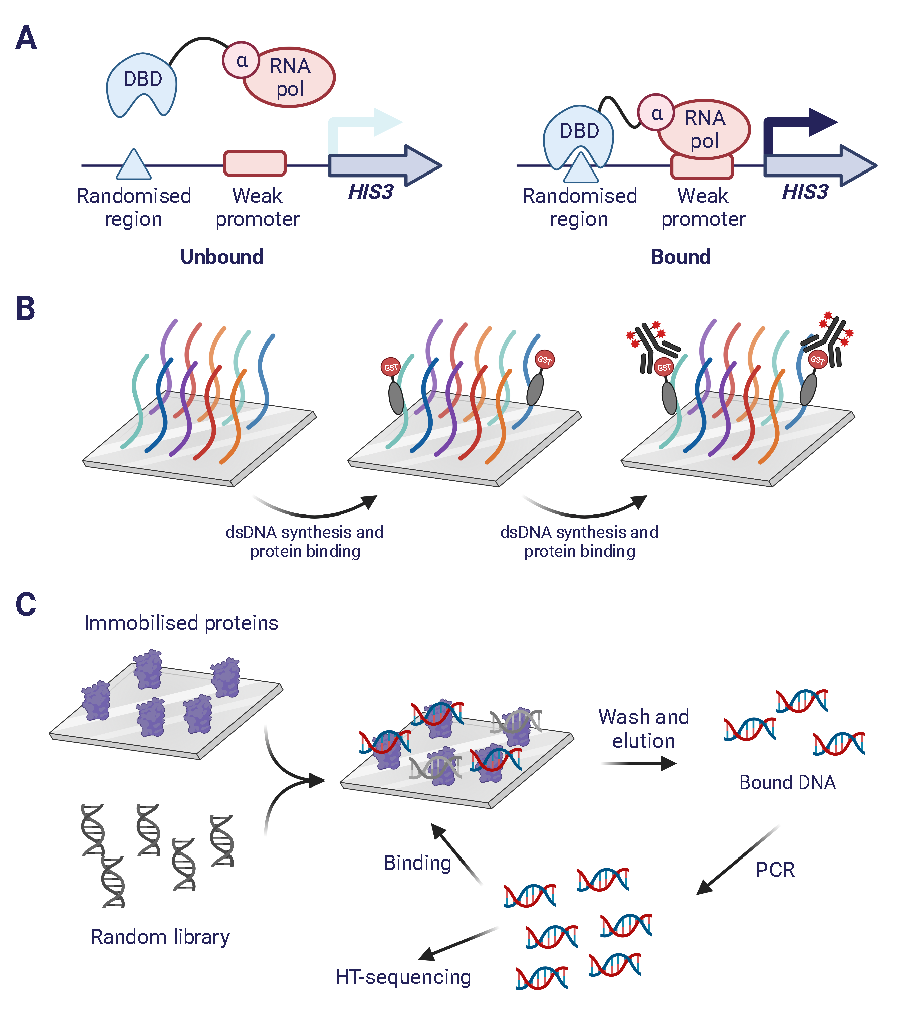
\includegraphics[width=0.9\textwidth]{chapter1/figures/fig7.pdf}
    \caption[Schematic views of three commonly-used high-throughput methods to study protein-DNA interactions \textit{in vitro}]{\textbf{Schematic views of three commonly-used high-throughput methods to study protein-DNA interactions \textit{in vitro}: B1H (A), PBM (B), and HT-SELEX (C).} See the main text for detailed descriptions (adapted from \cite{stormo2010determining}).}
    \label{fig:fig7}
\end{figure}

In the PBM, ssDNAs with common primers and spot-specific DNA sequences are immobilised on a microarray, and the ssDNAs are converted to dsDNA by extension using the common primer. The DBD of a transcription factor is fused to a tag (to date, only GST tag has been successfully used in the PBM) and purified. Then purified proteins are incubated with DNAs on the microarray, and the binding is visualised by incubating a fluorescence labelled antibody that recognises the tag (\textbf{Figure \ref{fig:fig7}B}). In this way, the binding of the transcription factor to all possible 10-mer sequences can be investigated.

HT-SELEX couples the traditional SELEX method with recent next generation sequencing technology. It utilises DNA ligands, each of which contains a 14-mer randomised DNA sequence, a 5-bp unique barcode and a universal sequencing primer for the high- throughput sequencing (usually an Illumina primer). The DNA ligands containing all possible 14-mer sequences are incubated with purified proteins immobilised to a 96-well plate. After washing off non-specific binding and elution, the bound DNA sequences are amplified and sequenced by high-throughput sequencing (\textbf{Figure \ref{fig:fig7}C}). HT-SELEX only requires a small amount of proteins (low nanogram levels), which is compatible with mammalian expression systems. Therefore, investigating the DNA binding of full-length proteins and proteins carrying post-translational modifications is possible.

\subsubsection{\textit{In vivo} methods}

\textit{In vitro} methods have generated valuable information, but \textit{in vitro} binding does not necessarily reflect \textit{in vivo} binding events. Fortunately, recent advances in chromatin immunoprecipitation (ChIP) followed by microarray (ChIP-chip) or by next generation sequencing (ChIP-seq) have enabled us to create a snapshot of the genome-wide binding profile of a specific transcription factor in a given cell type in a single experiment (reviewed in \cite{farnham2009insights}).

The first step of both ChIP-chip and ChIP-seq is the traditional ChIP assay: a protein of interest is covalently crosslinked to its DNA-binding sites or to another protein which directly contacts the DNA using crosslinkers, usually formaldehyde. After the shearing of the chromatin by sonication or enzymatic digestion, an antibody specific to the protein of interest is used to immunoprecipitate the protein-DNA adduct. After washing off the non- specific proteins bound by the antibody, the precipitated DNA fragments are reverse- crosslinked and purified. For ChIP-chip, the DNA samples are labelled with fluorescent dye and hybridised to designed microarrays (\textbf{Figure \ref{fig:fig8}}). For ChIP-seq, the sample is used to create a library that will be analysed by high-throughput next generation sequencing. The 5’ end of the DNA library is sequenced, and the resulting short sequencing reads, also known as tags (the terms reads and tags are interchangeable), are mapped back to a reference genome to identify the positions of the reads (\textbf{Figure \ref{fig:fig8}}). Then both methods require certain computational algorithms to detect the binding sites of the protein of interest (reviewed in \cite{park2009chip-seq:}).

\begin{figure}[h]
    \centering
    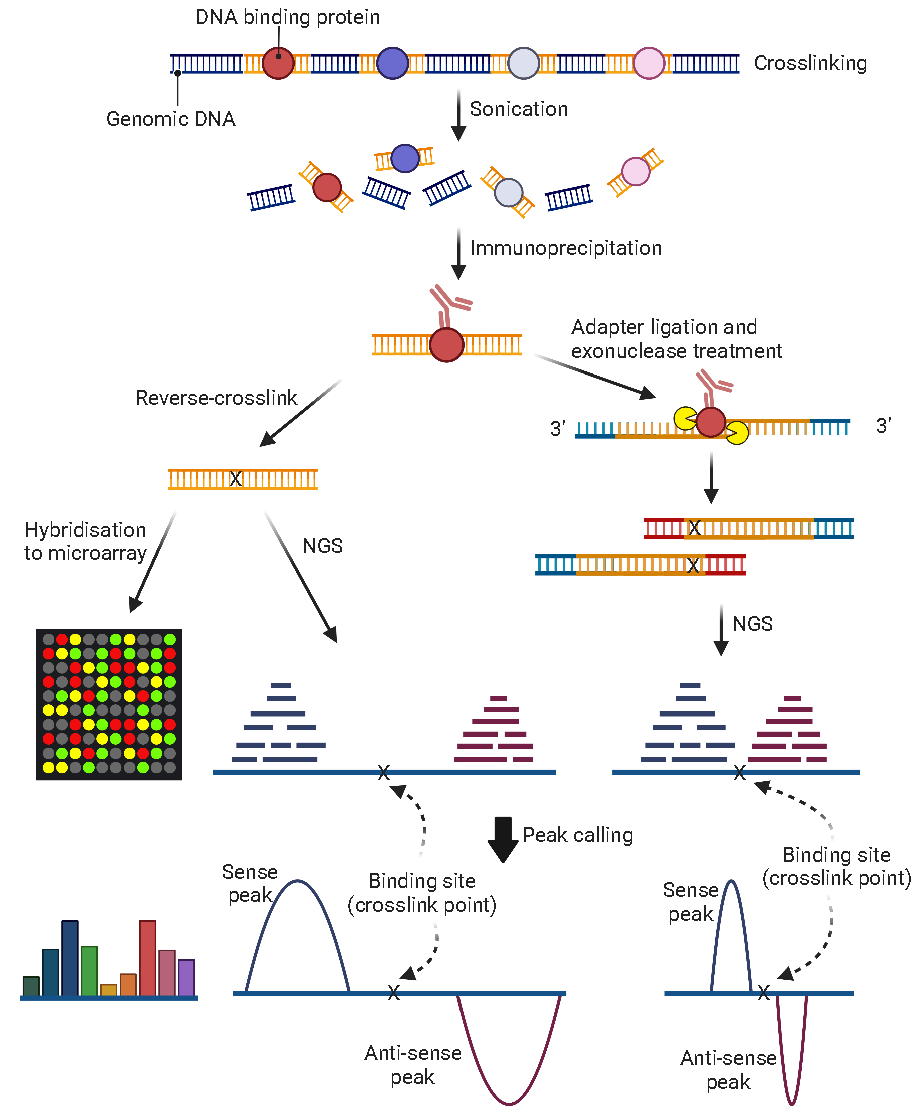
\includegraphics[width=0.8\textwidth]{chapter1/figures/fig8.pdf}
    \caption[Schematic views of the procedures of three ChIP-based technologies to study protein-DNA interactions \textit{in vivo}]{\textbf{Schematic views of the procedures of three ChIP-based technologies to study protein-DNA interactions \textit{in vivo.}} See detailed descriptions in the main text (adapted from \cite{visel2009genomic,rhee2011comprehensive}).}
    \label{fig:fig8}
\end{figure}

The quality of ChIP-chip results depend on the coverage, density and resolution of the microarray used for hybridisation (reviewed in \cite{hudson2006high-throughput}). The sequence covered in a single microarray is fairly limited compared to the large scale of the human genome, and the resolution as well as clarity of signal is often quite poor. As an alternative method, ChIP-seq offers many advantages over ChIP-chip, such as higher resolution and signal-to-noise ratio, and greater coverage (reviewed in \cite{park2009chip-seq:}). Hence, ChIP-seq is gradually replacing ChIP-chip. However, when investigating organisms with small genomes or a specific part of a large genome, ChIP-chip is still useful and more cost-effective.

Although ChIP-seq has higher resolution and signal-to-noise ratio than ChIP-chip, the binding events identified from ChIP-seq experiment are still too large to identify the exact binding sites of a protein due to the heterogeneous DNA fragments generated by the sonication. Another serious issue is that the contamination of non-crosslinked DNA in the ChIP samples, meaning the majority (60 - 90\%) of the sequencing readout is background (\cite{pepke2009computation,rhee2011comprehensive}). To improve the resolution and to reduce the background of ChIP-seq, a recent study applies an exonuclease to the ChIP sample before reverse-crosslinking, where the exonuclease trims the 5’ of the DNA to the exact crosslinking point (\textit{i.e.} the exact binding site) (\textbf{Figure \ref{fig:fig8}}). In addition, the non-crosslinked DNA will be degraded, and hence the background will be reduced. When proceeding to the sequencing step, the resulting short sequencing reads are just flanking the exact crosslinked site. This method, called ChIP-exo, significantly increases the resolution and reduces the background of ChIP-seq, and has been successfully used in both yeast and human cells, and for factors both directly and indirectly bind to DNA (\cite{rhee2011comprehensive,rhee2012genome-wide,yen2012genome-wide}).

All ChIP-based methods are exclusively dependent on high-quality antibodies which are not always available. Indeed, according to a recent assessment of the quality of histone modification antibodies, more than 20\% fail in ChIP (\cite{egelhofer2011an}). The available antibodies for transcription factors are much fewer than those for histone modifications. To circumvent the antibody issues, a method, called DamID, has been developed to identify the \textit{in vivo} protein-DNA interaction (\cite{van-steensel2000identification}). In the DamID, the protein of interest is fused to the bacterial Dam methyltransferase. When the protein binds to DNA, it also brings the Dam methyltransferase close to DNA where it can methylate the adenine of the GATC sequence nearby. Instead of using specific antibodies, one can identify the binding events by finding out the G\sus{m}ATC sequences which does not exist in the eukaryotic genome without introducing the Dam methyltransferase (\cite{van-steensel2000identification}). However, the resolution of this method depends on the frequency of the GATC tetramer site in the genome, and it cannot detect the dynamic binding between protein and DNA, \textit{i.e.} when the protein dissociates from the DNA, the methylated adenine will still be present. Therefore, the ChIP-based methods are still the golden standard for the study of \textit{in vivo} protein-DNA interactions.


\subsubsection{DNA binding by Forkhead transcription factors}

Early low-throughput \textit{in vitro} experiments, using selection of binding sites from pools of short random-sequence duplexes (\cite{pierrou1995selection}), revealed a seven-nucleotide core sequence as the Forkhead transcription factors binding sites. This consensus core that is recognised by the Forkhead domain is RYMAAYA, where R represents an A or G, Y represents a C or T, and M represents an A or C (\cite{kaufmann1995dna,overdier1994the,pierrou1994cloning}). Detailed comparison among the binding sites of FOXF2, FOXC1, FOXD1 and FOXL1 indicates that sequences both within and flanking the Forkhead consensus further determine the binding specificity of individual Forkhead transcription factors. Within the RYMAAYA core consensus, the heptameric sequence GTAAACA is the highest affinity site in most cases, except that FOXL1 prefers ATAAACA, and FOXC1 prefers GTAAATA (\cite{pierrou1994cloning}). At the flanking bases, the sequence preference of individual FOX proteins is relatively more variable than that within the core consensus. The flanking sequences also seem to be very important in the DNA-binding events of FOX proteins, because changes of the flanking sequences lead to different binding affinities for FOX proteins, or even failure to bind FOX proteins in spite of the presence of the core consensus (\cite{pierrou1994cloning}). Another study which compares the binding sites of FOXA, FOXQ1 and FOXD3 also confirms the observation that sequences within and flanking the core consensus determine the binding specificity of different Forkhead transcription factors (\cite{overdier1994the}). This is not a new discovery, because similar situations also exist in other proteins, such as the homeobox proteins and ETS-domain proteins, where specificity appears to be governed by nucleotides flanking their core consensus (\cite{ekker1991optimal,ekker1992differential,catron1993nucleotides,szymczyna2000dna}).

The third $\alpha$-helix $\alpha 3$ is the main DNA contact interface of Forkhead transcription factors, and the amino acids within this region are extremely conserved (reviewed in \cite{hannenhalli2009the}). Some Forkhead transcription factors (\textit{e.g.} FOXA3 and FOXD3) possess an almost identical recognition helix $\alpha 3$ and even use a similar mechanism for DNA recognition (reviewed in \cite{obsil2008structure/function}), but they still possess different DNA sequence preferences (\cite{overdier1994the}). It has been shown that these differences arise from less conserved regions outside of the main DNA-binding interface. The use of domain-swap chimeric proteins suggests that amino acids around the N-terminal border of helix $\alpha 3$ and in the wing W2 of the FOX domain determine, at least in part, the specificity (\cite{pierrou1994cloning}). Consistent with this discovery, another study used a series of HFH/HNF-3 protein chimeras and uncovered a 20-amino-acid region, which resides adjacent to the recognition helix $\alpha 3$, as responsible for determining their DNA-binding specificity (\cite{overdier1994the}). It is worth mentioning that a similar situation was also observed in ETS-domain proteins, where amino acid residues located away from the DNA- binding interface are found to be critical determinants for the binding specificity of individual ETS transcription factors (\cite{shore1996determinants}).

Recent high-throughput \textit{in vitro} experiments are consistent with previous findings. The DNA binding of mouse Forkhead transcription factors FOXA2, FOXJ1, FOXJ3, FOXK1 and FOXL1 have been analysed by PBM, and human FOXJ3 has been analysed by HT-SELEX. The core consensus RYMAAYA is the most frequent bound sequence, with GTAAACA being the highest affinity site in all cases. However, no apparent sequence preference for individual factor is observed (\cite{badis2009diversity,jolma2010multiplexed}).

Several human Forkhead transcription factors like FOXA (\cite{hurtado2011foxa1,motallebipour2009differential}), FOXH (\cite{kim2011chromatin}), FOXK (\cite{grant2012live-cell,ji2012the}) and FOXP (\cite{gabut2011an,katoh2011foxp3}) have been studied only recently by the ChIP-seq analyses. Motif searches reveal that responsive elements that resemble the Forkhead core consensus are enriched in the cistromes of all those factors. However, due to the differences of cell lines and computational algorithms used in different labs, it is difficult to explore the binding specificity of those Forkhead proteins. On the other hand, all of these studies have mainly focused on finding potential target genes and functions of individual Forkhead transcription factor, and none of these highlights the binding specificity of them.

Therefore, to explore the in vivo DNA binding specificity of individual Forkhead transcription factor, and more importantly to investigate the developmental and biological consequences of the binding specificity, it is better to perform ChIP-seq experiments of different members in the same cell line, and use the same computational approach to compare their DNA binding events.

\pagebreak

\section{Aims of the PhD project}

The healthy development of a living cell requires precise spatial-temporal gene expression. The first step of gene expression is transcription, which plays a central part in controlling the spatial-temporal gene expression. The general goal of studying transcription is to get an overall picture of how the whole transcriptional network controls gene expression, where transcription factors binding to DNA is a crucial step. To achieve this goal, one of the daunting challenges that we have to face is to understand the mechanisms of binding specificity of transcription factors. The overall aim of the project was to further our understanding of how transcription factors specifically recognise their target sites in the genome, when multiple family members can potentially converge on DNA sites with very similar sequences. Moreover, this then impacts on our ability to understand how a specific gene expression pattern can be generated in response to specific signals through a particular transcription factor. As a model system, we studied Forkhead transcription factors and in particular, the subgroup that impact on the cell cycle, especially on the G2 and M phases -- FOXK2, FOXM1 and FOXO3 transcription factors, all of which are ubiquitously expressed across a wide range of tissues and have their own specific functions. We chose to study their genome-wide binding events in the human osteosarcoma cell line U2OS, because it is a well-defined model cell line for the study of regulation of the cell cycle. Key questions that needed to be investigated include:

\begin{itemize}
    \item where do FOXK2, FOXM1 and FOXO3 bind in the genome?
    \item how are their DNA-binding specificities achieved?
    \item how is the binding specificity influenced by signalling pathways?
    \item how is the binding specificity related to their subsequent biological functions?
\end{itemize}

\chapter{Material and Methods} \label{ch:mm}

\section{Material}

General laboratory reagents and chemicals are purchased from Sigma-Aldrich, Invitrogen, Roche-Applied-Science, Promega and Serva.

\subsection{Buffers and solutions}

Highly purified water (Milli-Q biocel-dispenser) is used for all reactions described and for preparation of buffers and solutions. Buffers and solutions not listed are described in the appropriate methods section.

{\small
\begin{longtable}{|>{\centering\arraybackslash}m{5.25cm}|>{\raggedright\arraybackslash}m{5.5cm}|>{\centering\arraybackslash}b{3.5cm}|}
    %% table setup %%
    \caption{Buffers and solutions for cell lysis, gel electrophoresis, and western blot\label{table:wb}}\\
    \hline
    \textbf{Name} & \textbf{Ingredients} & \textbf{Final concentration}\\
    \hline
    \endfirsthead
    \multicolumn{3}{l}{\textbf{\textit{Table \ref{table:wb}}} continued}\\
    \hline
    \textbf{Name} & \textbf{Ingredients} & \textbf{Final concentration}\\
    \hline
    \endhead
    \hline
    \multicolumn{3}{l}{\textit{continued on the next page}}\\
    \endfoot
    \hline \hline
    \endlastfoot
    
    %% actual content %%
    \multirow{7}{4.25cm}{\centering \textbf{Triton Lysis Buffer}} & Tris-HCl, pH 7.4 & 20 mM\\
        & NaCl & 137 mM\\
        & EDTA & 2 mM\\
        & Dithiothreitol (DTT) & 0.5 mM\\
        & Glycerol & 10\% (w/v)\\
        & Triton X-100 & 1\% (v/v)\\
        & Protease Inhibitor Cocktail & 1x\\
    \hline
    \multirow{5}{4.25cm}{\centering \textbf{Triton Lysis Buffer} (with phosphatase inhibitors)} 
        & \textbf{Triton Lysis Buffer} supplied with the following: & $\ $\\
        & Sodium $\beta$-glycerophosphate                           & 0.5 M\\
        & Sodium pyrophosphate                                      & 2 mM\\
        & NaF                                                       & 50 mM\\
        & Na\sub{3}VO\sub{4}                                        & 1 mM\\
        \hline
    \multirow{6}{4.25cm}{\centering \textbf{SDS PAGE Loading Buffer} (5$\times$)}
        & Tris-HCl, pH 6.8              & 210 mM\\
        & Sodium dodecyl sulphate (SDS) & 10\% (w/v)\\
        & Glycerol                      & 21.6\% (w/v)\\
        & Dithiothreitol (DTT)          & 5.6\% (w/v)\\
        & Bromophenol blue              & 0.002\% (w/v)\\
        & $\beta$-Mercaptoethanol       & 10\% (v/v)\\
    \hline
    \multirow{2}{4.25cm}{\centering \textbf{Polyacrylamide Gel Lower Buffer} (4$\times$)}
        & Tris-HCl, pH 8.8 & 1.5 M\\
        & SDS              & 0.4\% (w/v)\\
    \hline
    \multirow{2}{4.25cm}{\centering \textbf{Polyacrylamide Gel Upper Buffer} (4$\times$)}
        & Tris-HCl, pH 6.8 & 0.5 M\\
        & SDS              & 0.4\% (w/v)\\
    \hline
    \multirow{3}{4.25cm}{\centering \textbf{SDS Running Buffer} (10$\times$)}
        & Tris-base & 250 mM\\
        & Glycine   & 1.9 M\\
        & SDS       & 0.1\% (w/v)\\
    \hline
    \multirow{3}{4.25cm}{\centering \textbf{Wet Transfer Buffer} (1$\times$)}
        & Tris-base & 25 mM\\
        & Glycine   & 190 mM\\
        & Methanol  & 20\% (v/v)\\ 
    \hline
    \textbf{Odyssey Blocking Buffer} & N.A. & N.A.\\
    \hline
    \multirow{3}{4.25cm}{\centering \textbf{Phosphate-Buffered Saline} (PBS) (1$\times$), pH 7.4}
        & NaCl      & 137 mM\\
        & Phosphate & 10 mM\\
        & KCl       & 2.7 mM\\
    \hline
    \multirow{2}{4.25cm}{\centering \textbf{Tris-Buffered Saline} (TBS) (1$\times$), pH 8.0}
        & Tris-base & 50 mM\\
        & NaCl      & 150 mM\\
    \hline
    \pagebreak
    \multirow{3}{4.25cm}{\centering \textbf{TBS-Tween} (1$\times$), pH 8.0}
        & Tris-base & 50 mM\\
        & NaCl      & 150 mM\\
        & Tween-20  & 0.05\% (v/v)\\
    \hline
    \multirow{3}{4.25cm}{\centering \textbf{Coomassie blue stain}}
        & Coomassie brilliant blue R250 & 0.25\% (w/v)\\
        & Acetic acid                   & 10\% (v/v)\\
        & Methanol                      & 45\% (v/v)\\
    \hline
    \multirow{2}{4.25cm}{\centering \textbf{Destain solution}}
        & Acetic acid & 10\% (v/v)\\
        & Methanol    & 45\% (v/v)\\
    \hline
\end{longtable}

\begin{longtable}{|>{\centering\arraybackslash}m{5.25cm}|>{\raggedright\arraybackslash}m{5.5cm}|>{\centering\arraybackslash}b{3.5cm}|}
    %% table setup %%
    \caption{Buffers and solutions for Chromatin Immunoprecipitation\label{table:chip}}\\
    \hline
    \textbf{Name} & \textbf{Ingredients} & \textbf{Final concentration}\\
    \hline
    \endfirsthead
    \multicolumn{3}{l}{\textbf{\textit{Table \ref{table:chip}}} continued}\\
    \hline
    \textbf{Name} & \textbf{Ingredients} & \textbf{Final concentration}\\
    \hline
    \endhead
    \hline
    \multicolumn{3}{l}{\textit{continued on the next page}}\\
    \endfoot
    \hline \hline
    \endlastfoot
    
    %% actual content %%
    \multirow{2}{4.25cm}{\centering \textbf{Crosslinking Solution}}
        & PBS, pH 7.4  & 1$\times$\\
        & Formaldehyde & 1\% (v/v)\\
    \hline
    \multirow{2}{4.25cm}{\centering \textbf{Quenching Solution}}
        & PBS, pH 7.4 & 1$\times$\\
        & Glycine.    & 125 mM\\
    \hline
    \multirow{2}{4.25cm}{\centering \textbf{ChIP Blocking Buffer}}
        & PBS, pH 7.4                & 1$\times$\\
        & Bovine Serum Albumin (BSA) & 0.5\% (w/v)\\
    \hline
    \multirow{6}{4.25cm}{\centering \textbf{ChIP Lysis Buffer I}}
        & HEPES, pH 7.5 & 50 mM\\
        & NaCl          & 140 mM\\
        & EDTA, pH 8.0  & 1 mM\\
        & Glycerol      & 10\% (v/v)\\
        & IGEPAL CA-630 & 0.5\% (v/v)\\
        & Triton X-100  & 0.25\% (v/v)\\
        \hline
    \multirow{4}{4.25cm}{\centering \textbf{ChIP Lysis Buffer II}}
        & Tris-HCl, pH 8.0 & 10 mM\\
        & NaCl             & 200 mM\\
        & EDTA, pH 8.0     & 1 mM\\
        & EGTA, pH 8.0     & 0.5 mM\\
    \hline
    \pagebreak
    \multirow{6}{4.25cm}{\centering \textbf{ChIP Lysis Buffer III}}
        & Tris-HCl, pH 8.0      & 10 mM\\
        & NaCl                  & 100 mM\\
        & EDTA, pH 8.0          & 1 mM\\
        & EGTA, pH 8.0          & 0.5 mM\\
        & Na Deoxycholate (DOC) & 0.1\% (w/v)\\
        & N-lauroyl sarcosine   & 0.5\% (w/v)\\
    \hline
    \multirow{5}{4.25cm}{\centering \textbf{ChIP RIPA Wash Buffer}}
        & HEPES, pH 7.5         & 50 mM\\
        & LiCl                  & 500 mM\\
        & EDTA, pH 8.0          & 1 mM\\
        & IGEPAL CA-630         & 1\% (v/v)\\
        & Na Deoxycholate (DOC) & 0.7\% (w/v)\\
    \hline
    \multirow{3}{4.25cm}{\centering \textbf{ChIP Elution Buffer}}
        & Tris-HCl, pH 8.0 & 50 mM\\
        & EDTA, pH 8.0     & 10 mM\\
        & SDS              & 1\% (w/v)\\
    \hline
    \multirow{3}{4.25cm}{\centering \textbf{1$\times$ TE + 50 mM NaCl}}
        & Tris-HCl, pH 8.0 & 10 mM\\
        & EDTA, pH 8.0     & 1 mM\\
        & NaCl             & 50 mM\\
    \hline
    \multirow{2}{4.25cm}{\centering \textbf{TE} (1$\times$)}
        & Tris-HCl, pH 8.0 & 10 mM\\
        & EDTA, pH 8.0     & 1 mM\\
    \hline
\end{longtable}

\begin{longtable}{|>{\centering\arraybackslash}m{4.25cm}|>{\raggedright\arraybackslash}m{6.5cm}|>{\centering\arraybackslash}b{3.5cm}|}
    %% table setup %%
    \caption{Buffers and solutions for Band shift\label{table:bandshift}}\\
    \hline
    \textbf{Name} & \textbf{Ingredients} & \textbf{Final concentration}\\
    \hline
    \endfirsthead
    \multicolumn{3}{l}{\textbf{\textit{Table \ref{table:bandshift}}} continued}\\
    \hline
    \textbf{Name} & \textbf{Ingredients} & \textbf{Final concentration}\\
    \hline
    \endhead
    \hline
    \multicolumn{3}{l}{\textit{continued on the next page}}\\
    \endfoot
    \hline \hline
    \endlastfoot
    
    %% actual content %%
    \multirow{6}{4.25cm}{\centering \textbf{Dz Buffer} (1$\times$)}
        & HEPES-KOH, pH 7.9  & 25 mM\\
        & Glycerol           & 20\% (v/v)\\
        & MgCl\sub{2}        & 2 mM\\
        & DTT                & 1 mM\\
        & ZnCl\sub{2}        & 0.1 $\mu$M\\
        & EDTA, pH 8.0       & 0.2 mM\\
    \hline
    \pagebreak
    \multirow{2}{4.25cm}{\centering \textbf{FpF Buffer} (4$\times$)}
        & Spermidine   & 8 mM\\
        & EDTA, pH 8.0 & 9.4 mM\\
    \hline
    \multirow{3}{4.25cm}{\centering \textbf{Sample Dilution Buffer}}
        & PBS, pH 7.4 & 1$\times$\\
        & Glycerol    & 10\% (v/v)\\
        & BSA         & 1 mg/mL (w/v)\\
    \hline
    \multirow{4}{4.25cm}{\textbf{\centering Band shift Loading Buffer}}
        & Ficoll 400                         & 8\% (w/v)\\
        & TE                                 & 0.5$\times$\\
        & EDTA, pH 8.0                       & 70 mM\\
        & Xylene cyanol and Bromophenol blue & 0.1\% (v/v)\\
    \hline
\end{longtable}

\begin{longtable}{|>{\centering\arraybackslash}m{4.25cm}|>{\raggedright\arraybackslash}m{6.5cm}|>{\centering\arraybackslash}b{3.5cm}|}
    %% table setup %%
    \caption{Buffers and solutions for other uses\label{table:others}}\\
    \hline
    \textbf{Name} & \textbf{Ingredients} & \textbf{Final concentration}\\
    \hline
    \endfirsthead
    \multicolumn{3}{l}{\textbf{\textit{Table \ref{table:others}}} continued}\\
    \hline
    \textbf{Name} & \textbf{Ingredients} & \textbf{Final concentration}\\
    \hline
    \endhead
    \hline
    \multicolumn{3}{l}{\textit{continued on the next page}}\\
    \endfoot
    \hline \hline
    \endlastfoot
    
    %% actual content %%
    \multirow{4}{4.25cm}{\centering \textbf{Agarose Gel Loading Buffer} (6$\times$)}
        & Bromophenol blue & 0.25\% (w/v)\\
        & Xylene cyanol    & 0.25\% (w/v)\\
        & EDTA, pH 8.0     & 30 mM\\
        & Glycerol         & 60\% (v/v)\\
    \hline
    \multirow{3}{4.25cm}{\centering \textbf{Biotin Binding Buffer} (1$\times$)}
        & Tris-HCl, pH 8.0 & 10 mM\\
        & EDTA, pH 8.0     & 1 mM\\
        & NaCl             & 2 M\\
    \hline
    \multirow{2}{4.25cm}{\centering \textbf{Biotin Elution Buffer}}
        & Formamide     & 95\% (v/v)\\
        & EDTA, pH 8.0  & 10 mM\\
    \hline
    \multirow{6}{4.25cm}{\centering \textbf{HKMG Buffer}}
        & HEPES-KOH, pH 7.9 & 10 mM\\
        & KCl               & 100 mM\\
        & MgCl\sub{2}       & 5 mM\\
        & Glycerol          & 10\% (v/v)\\
        & IGEPAL CA-630     & 0.5\% (v/v)\\
        & DTT               & 1 mM\\
    \hline
    \pagebreak
    \multirow{3}{4.25cm}{\centering \textbf{TAE} (1$\times$)}
         & Tris-base           & 40 mM\\
         & Glacial acetic acid & 0.1\% (v/v)\\
         & EDTA, pH 8.0        & 1 mM\\
    \hline
    \multirow{3}{4.25cm}{\centering \textbf{TBE} (1$\times$)}
         & Tris-base    & 89 mM\\
         & Boric acid   & 89 mM\\
         & EDTA, pH 8.0 & 2 mM\\
    \hline
    \multirow{3}{4.25cm}{\centering \textbf{Ni Binding Buffer} (8$\times$)}
         & Imidazole        & 40 mM\\
         & NaCl             & 4 M\\
         & Tris-HCl, pH 7.9 & 160 mM\\
    \hline
    \multirow{3}{4.25cm}{\centering \textbf{Ni Wash Buffer} (8$\times$)}
         & Imidazole        & 480 mM\\
         & NaCl             & 4 M\\
         & Tris-HCl, pH 7.9 & 160 mM\\
    \hline
    \multirow{3}{4.25cm}{\centering \textbf{Ni Elution Buffer} (4$\times$)}
         & Imidazole        & 4 M\\
         & NaCl             & 2 M\\
         & Tris-HCl, pH 7.9 & 80 mM\\
    \hline
    \multirow{5}{4.25cm}{\centering \textbf{Pulldown Buffer} (1$\times$)}
         & Tris-HCl, pH 7.4 & 50 mM\\
         & NaCl             & 150 mM\\
         & Glycerol         & 5\% (v/v)\\
         & IGEPAL CA-630    & 0.2\% (v/v)\\
         & DTT              & 0.5 mM\\
    \hline
    \multirow{4}{4.25cm}{\centering \textbf{CoIP Buffer} (1$\times$)}
         & HEPES-KOH, pH 7.4 & 50 mM\\
         & NaCl              & 150 mM\\
         & MgCl\sub{2}       & 1 mM\\
         & TWEEN-20          & 1\% (v/v)\\
    \hline
\end{longtable}
}

\pagebreak

\subsection{Enzymes}

{\small
\begin{longtable}{|>{\raggedright\arraybackslash}m{4cm}|>{\raggedright\arraybackslash}m{7cm}|}
    %% table setup %%
    \caption{Enzymes used in this study\label{table:enzymes}}\\
    \hline
    \textbf{Name} & \textbf{Supplier (Catalogue Number)}\\
    \hline
    \endfirsthead
    \multicolumn{2}{l}{\textbf{\textit{Table \ref{table:enzymes}}} continued}\\
    \hline
    \textbf{Name} & \textbf{Supplier (Catalogue Number)}\\
    \hline
    \endhead
    \hline
    \multicolumn{2}{l}{\textit{continued on the next page}}\\
    \endfoot
    \hline \hline
    \endlastfoot
    
    %% actual content %%
    Restriction Enzymes        & New England Biolabs\\
    \hline
    Ribonuclease A             & Sigma-Aldrich (R-6513)\\
    \hline
    T4 DNA Ligase              & Invitrogen (15224-041)\\
    \hline
    Pfu-DNA Polymerase         & Stratagene (600135-12)\\
    \hline
    Lambda Protein Phosphatase & New England Biolabs (P0735S)\\
    \hline
    Proteinase K               & Roche Applied Science (03115887001)\\
    \hline
\end{longtable}
}

\subsection{Antibodies}

{\small
\begin{longtable}{|>{\centering\arraybackslash}m{1.9cm}|>{\centering\arraybackslash}m{1.4cm}|>{\centering\arraybackslash}m{2cm}|>{\centering\arraybackslash}m{1.6cm}|>{\raggedright\arraybackslash}m{6.5cm}|}
    %% table setup %%
    \caption{Primary Antibodies used in western blot\label{table:wbab}}\\
    \hline
    \textbf{Antibody} & \textbf{Raised in} & \textbf{Clonality} & \textbf{Dilution for WB} & \textbf{Supplier (Catalogue Number)}\\
    \hline
    \endfirsthead
    \multicolumn{5}{l}{\textbf{\textit{Table \ref{table:wbab}}} continued}\\
    \hline
    \textbf{Antibody} & \textbf{Raised in} & \textbf{Clonality} & \textbf{Dilution for WB} & \textbf{Supplier (Catalogue Number)}\\
    \hline
    \endhead
    \hline
    \multicolumn{5}{l}{\textit{continued on the next page}}\\
    \endfoot
    \hline \hline
    \endlastfoot
    
    %% actual content %%
    \textbf{Cyclin B} (GNS1) & Mouse  & Monoclonal & 1:1000 & Santa Cruz Biotech. (sc-245)\\
    \hline
    \textbf{E2F4} (C-20)     & Rabbit & Polyclonal & 1:1000 & Santa Cruz Biotech. (sc-866)\\
    \hline
    \textbf{ERK2} (C-14)     & Rabbit & Polyclonal & 1:1000 & Santa Cruz Biotech. (sc-154)\\
    \hline
    \textbf{FLAG} M2         & Mouse  & Monoclonal & 1:5000 & Sigma-Aldrich (F3165)\\
    \hline
    \textbf{FOXK2}           & Rabbit & Polyclonal & 1:1000 & Bethyl Laboratories (A301-729A)\\
    \hline
    \textbf{FOXM1} (C-20)    & Rabbit & Polyclonal & 1:1000 & Santa Cruz Biotech. (sc-502)\\
    \hline
    \textbf{FOXM1}           & Rabbit & Polyclonal & 1:1000 & Cell Signalling Technology (\#3948)\\
    \hline
    \textbf{FOXO3} (75D8)    & Rabbit & Monoclonal & 1:1000 & Cell Signalling Technology (\#2497)\\
    \hline
    \textbf{FOXO3}           & Rabbit & Polyclonal & 1:2500 & Millipore (07-702)\\
    \hline
    \textbf{GFP}             & Rabbit & Polyclonal & 1:1000 & Santa Cruz Biotech. (sc-8334)\\
    \hline
    \textbf{Lamin B} (C-20)  & Goat   & Polyclonal & 1:1000 & Santa Cruz Biotech. (sc-6216)\\
    \hline
    \textbf{MYBL2} (C-20)    & Rabbit & Polyclonal & 1:1000 & Santa Cruz Biotech. (sc-725)\\
    \hline
    \textbf{NF-YA} (H-209)   & Rabbit & Polyclonal & 1:1000 & Santa Cruz Biotech. (sc-10779)\\
    \hline
    \textbf{pAkt} (Ser473)   & Rabbit & Polyclonal & 1:1000 & Cell Signalling Technology (\#9271)\\
    \hline
    \textbf{SRF} (G-20)      & Rabbit & Polyclonal & 1:1000 & Santa Cruz Biotech. (sc-335)\\
    \hline
    \textbf{$\beta$-Tubulin} & Rabbit & Polyclonal & 1:1000 & Abcam (ab6046)\\
    \hline
    \textbf{V5}              & Mouse  & Monoclonal & 1:5000 & Sigma-Aldrich (V8012)\\
    \hline
\end{longtable}

\begin{longtable}{|>{\centering\arraybackslash}m{1.9cm}|>{\centering\arraybackslash}m{1.4cm}|>{\centering\arraybackslash}m{2cm}|>{\centering\arraybackslash}m{1.6cm}|>{\raggedright\arraybackslash}m{6.5cm}|}
    %% table setup %%
    \caption{Secondary Antibodies used in western blot\label{table:wbab2}}\\
    \hline
    \textbf{Antibody} & \textbf{Raised in} & \textbf{Clonality} & \textbf{Dilution for WB} & \textbf{Supplier (Catalogue Number)}\\
    \hline
    \endfirsthead
    \multicolumn{5}{l}{\textbf{\textit{Table \ref{table:wbab2}}} continued}\\
    \hline
    \textbf{Antibody} & \textbf{Raised in} & \textbf{Clonality} & \textbf{Dilution for WB} & \textbf{Supplier (Catalogue Number)}\\
    \hline
    \endhead
    \hline
    \multicolumn{5}{l}{\textit{continued on the next page}}\\
    \endfoot
    \hline \hline
    \endlastfoot
    
    %% actual content %%
    \small \setstretch{1} \textbf{IRDye 800CW anti-Mouse IgG}  & Goat   & Polyclonal & 1:10,000 & Li-Cor Biosciences (926-32210)\\
    \hline
    \small \setstretch{1} \textbf{IRDye 800CW anti-Rabbit IgG} & Goat   & Polyclonal & 1:10,000 & Li-Cor Biosciences (926-32211)\\
    \hline
    \small \setstretch{1} \textbf{IRDye 680LT anti-Mouse IgG}  & Donkey & Polyclonal & 1:20,000 & Li-Cor Biosciences (926-68022)\\
    \hline
    \small \setstretch{1} \textbf{IRDye 680LT anti-Rabbit IgG} & Donkey & Polyclonal & 1:20,000 & Li-Cor Biosciences (926-68023)\\
    \hline
    \small \setstretch{1} \textbf{IRDye 680LT anti-Goat IgG}   & Donkey & Polyclonal & 1:20,000 & Li-Cor Biosciences (926-68024)\\
    \hline
\end{longtable}

\begin{longtable}{|>{\raggedright\arraybackslash}m{4cm}|>{\raggedright\arraybackslash}m{7.5cm}|}
    %% table setup %%
    \caption{Antibodies used in Chromatin Immunoprecipitation\label{table:chipab}}\\
    \hline
    \textbf{Name} & \textbf{Supplier (Catalogue Number)}\\
    \hline
    \endfirsthead
    \multicolumn{2}{l}{\textbf{\textit{Table \ref{table:chipab}}} continued}\\
    \hline
    \textbf{Name} & \textbf{Supplier (Catalogue Number)}\\
    \hline
    \endhead
    \hline
    \multicolumn{2}{l}{\textit{continued on the next page}}\\
    \endfoot
    \hline \hline
    \endlastfoot
    
    % actual content
    FLAG M2 & Sigma-Aldrich (F3165)\\
    \hline
    FOXK2             & Bethyl Laboratories (A301-729A)\\
    \hline
    FOXM1 (C-20)      & Santa Cruz Biotech. (sc-502)\\
    \hline
    NF-YA (H-209)     & Santa Cruz Biotech. (sc-10779)\\
    \hline
    Normal Rabbit IgG & Millipore (\#12-370)\\
    \hline
    Normal Mouse IgG  & Millipore (\#12-371)\\
    \hline
\end{longtable}
}

\subsection{Chemicals used in cell cultures and treatments} \label{section:antibiotics}

{\small
\begin{longtable}{|>{\centering\arraybackslash}m{3cm}|>{\centering\arraybackslash}m{3cm}|>{\raggedright\arraybackslash}m{4.5cm}|>{\centering\arraybackslash}m{3cm}|}
    %% table setup %%
    \caption{Antibiotics and cell cycle synchronisation reagents\label{table:tc}}\\
    \hline
    \textbf{Name} & \textbf{Diluent} & \textbf{Supplier (Catalogue Number)} & \textbf{Final concentration}\\
    \hline
    \endfirsthead
    \multicolumn{4}{l}{\textbf{\textit{Table \ref{table:tc}}} continued}\\
    \hline
    \textbf{Name} & \textbf{Diluent} & \textbf{Supplier (Catalogue Number)} & \textbf{Final concentration}\\
    \hline
    \endhead
    \hline
    \multicolumn{4}{l}{\textit{continued on the next page}}\\
    \endfoot
    \hline \hline
    \endlastfoot
    
    %% actual content %%
    Blasticidin  & Sterilised Water & PAA (P05-017) & 10 $\mu$g/mL\\
    \hline
    Doxycycline  & Sterilised Water & Sigma-Aldrich (D9891) & 1.5 ng - 1 $\mu$g/ml\footnote{See \textbf{Results} section for the specific concentration for different applications.}\\
    \hline
    G-418        & HEPES            & PAA (P11-012)            & 500 $\mu$g/mL\\
    \hline
    Hydroxyurea  & Sterilised Water & Sigma-Aldrich (H8627)    & 5 mM\\
    \hline
    Hygromycin B & HEPES            & PAA (P02-015)            & 100 $\mu$g/mL\\
    \hline
    LY294002     & DMSO             & Merck Chemicals (440202) & 20 $\mu$M\\
    \hline
    Nocodazole   & DMSO             & Sigma-Aldrich (M1404)    & 100 nM\\
    \hline
    Puromycin    & Sterilised Water & PAA (P11-019)            & 1 $\mu$g/mL\\
    \hline
    Thymidine    & Sterilised Water & Sigma-Aldrich (T1895)    & 2 mM\\
    \hline
\end{longtable}
}

\subsection{Oligonucleotides}

{\footnotesize \setstretch{1}
\begin{longtable}{|>{\centering\arraybackslash}m{1cm}|>{\centering\arraybackslash}m{3.5cm}|>{\centering\arraybackslash}m{4.5cm}|>{\raggedright\arraybackslash}m{4.7cm}|}
    %% table setup %%
    \caption{Oligonucleotides for the construction of plasmids (restriction sites are underlined)\label{table:cloneoligo}}\\
    \hline
    \textbf{ADS\#} & \textbf{Name} & \textbf{Purpose of the oligonucleotides} & \textbf{Sequence (5'$\rightarrow$3')}\\
    \hline
    \endfirsthead
    \multicolumn{4}{l}{\textbf{\textit{Table \ref{table:cloneoligo}}} continued}\\
    \hline
    \textbf{ADS\#} & \textbf{Name} & \textbf{Purpose of the oligonucleotides} & \textbf{Sequence (5'$\rightarrow$3')}\\
    \hline
    \endhead
    \hline
    \multicolumn{4}{l}{\textit{continued on the next page}}\\
    \endfoot
    \hline \hline
    \endlastfoot
    
    %% actual content %%
    2731 & TEV-V5-His-F & To introduce XhoI site upstream of TEV sequence & GCAT\textbf{\underline{CTCGAG}}\seqsplit{GCCGGCGAGAACCTGTACTTC}\\
    \hline
    2732 & TEV-V5-His-R & To introduce 6$\times$His tag, XbaI site, and a stop codon downstream of V5 tag sequence & GCAT\underline{TCTAGA}\seqsplit{TTAGTGATGGTGATGGTGATGTCCTGT GGAGTCCAGGCCCAG}\\
    \hline
    2790 & HindIII-FOXO3 & To introduce HindIII site to 5' of FOXO3 ORF & GCAT\underline{AAGCTT}\seqsplit{GCCATGGCAGAGGCACCGGCTTCC}\\
    \hline
    2791 & FOXO3-XhoI & To introduce XhoI site to 3' of FOXO3 ORF & GCAT\underline{CTCGAG}\seqsplit{GCCTGGCACCCAGCTCTGAGATG}\\
    \hline
    2792 & NdeI-FOXK2-FK & To introduce NdeI site to 5' of FOXK2 Forkhead domain coding sequence & CTGCAT\underline{CATATG}\seqsplit{CCAGTGAAGGCCGTACAGCCACAC}\\
    \hline
    2793 & FOXK2-FK-XhoI & To introduce XhoI site to 3' of FOXK2 Forkhead domain coding sequence & GCAT\underline{CTCGAG}\seqsplit{TAGCTGCCGCTGGACGGTGATTAAG}\\
    \hline
    2800 & NdeI-FOXO3-FK & To introduce NdeI site to 5' of FOXO3 Forkhead domain coding sequence & CTGCAT\underline{CATATG}\seqsplit{GGGGCGGCTGGGGGCTCCGGG}\\
    \hline
    2801 & FOXO3-FK-XhoI & To introduce XhoI site to 3' of FOXO3 Forkhead domain coding sequence & GCAT\underline{CTCGAG}\seqsplit{GTTGCTATTGTCCATGGAGAC}\\
    \hline
    2812 & NdeI-FOXM1c-FK & To introduce NdeI site to 5' of FOXM1c Forkhead domain coding sequence & CTGCAT\underline{CATATG}\seqsplit{CCACCTGGAGCCCTTTGCGAG}\\
    \hline
    2813 & FOXM1c-FK-XhoI & To introduce XhoI site to 3' of FOXM1c Forkhead domain coding sequence & GTCA\underline{CTCGAG}\seqsplit{AGCCGCCAGGGGCAATGGC}\\
    \hline
    2884 & BglII-CCNB2 & To introduce BglII site to 5' of human CCNB2 promoter sequence & CTGCAT\underline{AGATCT}\seqsplit{CGTGTCTAAGAAAATTCAGCCAATG}\\
    \hline
    2885 & Luc2-XhoI & To introduce XhoI site to 3' of Luciferase gene Luc2 coding sequence & CTGCAT\underline{CTCGAG}\seqsplit{TTACACGGCGATCTTGCCGC}\\
    \hline
    2908 & EcoRI-FOXM1-F1 & To generate truncations of FOXM1B protein & AGCTAG\underline{GAATTC}\seqsplit{ATGAAAACTAGCCCCCGTCGG}\\
    \hline
    2909 & EcoRI-FOXM1-F117 & To generate truncations of FOXM1B protein & AGCTAG\underline{GAATTC}\seqsplit{CAGCCTCCAGGACTCCGGCC}\\
    \hline
    2910 & EcoRI-FOXM1-F235 & To generate truncations of FOXM1B protein & AGCTAG\underline{GAATTC}\seqsplit{GAGCGGCCACCCTACTCTTAC}\\
    \hline
    2911 & R367-FOXM1-XhoI & To generate truncations of FOXM1B protein & AGCTAG\underline{CTCGAG}\seqsplit{TTACTGGATAGGTACCAGGTATG}\\
    \hline
    2912 & R490-FOXM1-XhoI & To generate truncations of FOXM1B protein & AGCTAG\underline{CTCGAG}\seqsplit{TTACGAATCCTCCCAGGAGTGAG}\\
    \hline
    2913 & R748-FOXM1-XhoI & To generate truncations of FOXM1B protein & AGCTAG\underline{CTCGAG}\seqsplit{TTACTGTAGCTCAGGAATAAACTG}\\
    \hline
    2918 & R130-FOXM1-XhoI & To generate truncations of FOXM1B protein & AGCTAG\underline{CTCGAG}\seqsplit{TTAATCATAGCTGGTTTGGGTTTG}\\
    \hline
    2919 & R235-FOXM1-XhoI & To generate truncations of FOXM1B protein & AGCTAG\underline{CTCGAG}\seqsplit{TTACCGCTCAGACACAGAGTTCTG}\\
    \hline
    2920 & HindIII-FOXM1-F117 & To generate truncations of FOXM1B protein & AGCTAG\underline{AAGCTT}\seqsplit{CAGCCTCCAGGACTCCGGCCTC}\\
    \hline
    2921 & BamHI-FOXM1-R748 & To generate truncations of FOXM1B protein & AGCTAG\underline{GGATCC}\seqsplit{CTACTGTAGCTCAGGAATAAACTG}\\
    \hline
    2932 & EcoRI-FOXM1-F451 & To generate truncations of FOXM1B protein & AGCTAG\underline{GAATTC}\seqsplit{CCTGGGGAGGAAATGCCACAC}\\
    \hline
    2933 & FOXM1b-qc1-F & To generate L9A/L11A mutations of FOXM1B & \seqsplit{CTAGCCCCCGTCGGCCAGCCATTGCCAAAAGACGGAGGCTGCC}\\
    \hline
    2934 & FOXM1b-qc1-R & To generate L9A/L11A mutations of FOXM1B & \seqsplit{GGCAGCCTCCGTCTTTTGGCAATGGCTGGCCGACGGGGGCTAG}\\
    \hline
    2935 & FOXM1b-qc2-F & To generate F106A/L108A mutations of FOXM1B & \seqsplit{GTAGTGGGCCCAACAAAGCCATCGCCATCAGCTGTGGGGGAGC}\\
    \hline
    2936 & FOXM1b-qc2-R & To generate F106A/L108A mutations of FOXM1B & \seqsplit{GCTCCCCCACAGCTGATGGCGATGGCTTTGTTGGGCCCACTAC}\\
    \hline
\end{longtable}

\begin{longtable}{|>{\centering\arraybackslash}m{1cm}|>{\centering\arraybackslash}m{3cm}|>{\centering\arraybackslash}m{4.5cm}|>{\raggedright\arraybackslash}m{5.2cm}|}
    %% table setup %%
    \caption{Oligonucleotides for sequencing\label{table:seqoligo}}\\
    \hline
    \textbf{ADS\#} & \textbf{Name} & \textbf{Target} & \textbf{Sequence (5'$\rightarrow$3')}\\
    \hline
    \endfirsthead
    \multicolumn{4}{l}{\textbf{\textit{Table \ref{table:seqoligo}}} continued}\\
    \hline
    \textbf{ADS\#} & \textbf{Name} & \textbf{Target} & \textbf{Sequence (5'$\rightarrow$3')}\\
    \hline
    \endhead
    \hline
    \multicolumn{4}{l}{\textit{continued on the next page}}\\
    \endfoot
    \hline \hline
    \endlastfoot
    
    %% actual content %%
    186  & T7 primer       & T7 promoter                         & \scriptsize TTAATACGACTCACTAT\\
    \hline
    187  & GST-seq-For     & Glutathione S-transferase (GST) CDS & \scriptsize GGGCTGGCAAGCCACGTTTGGTG\\
    \hline
    1532 & BGH-seq-rev     & BGH polyA                           & \scriptsize TAGAAGGCACAGTCGAGG\\
    \hline
    2737 & FOXM1-Cter-seq  & FOXM1 C-terminal                    & \scriptsize TTTGGCAACTCTTCTCCCTC\\
    \hline
    2886 & FOXM1-FK-seq T7 & FOXM1 Forkhead domain               & \scriptsize TGGCAGAACTCTGTGTCTGAG\\
    \hline
    2889 & terminator      & T7 terminator                       & \scriptsize TATGCTAGTTATTGCTCAG\\
    \hline
    2920 & GST-seq-rev     & Glutathione S-transferase (GST) CDS & \scriptsize AGCTGTGACCGTCTCCGGGAG\\
    \hline
    2890 & CMV forward     & CMV promoter                        & \scriptsize CGCAAATGGGCGGTAGGCGTG\\
    \hline
    3541 & Luc2-seq-F      & Luc2 gene body                      & \scriptsize GTAAGACACTGGGTGTGAACC\\
    \hline
\end{longtable}

\begin{longtable}{|>{\centering\arraybackslash}m{1cm}|>{\centering\arraybackslash}m{3cm}|>{\centering\arraybackslash}m{4.3cm}|>{\raggedright\arraybackslash}m{5.4cm}|}
    %% table setup %%
    \caption{Oligonucleotides for Chromatin Immunoprecipitation\label{table:chipoligo}}\\
    \hline
    \textbf{ADS\#} & \textbf{Name} & \textbf{Genomic coordinates (NCBI36/hg18)} & \textbf{Sequence (5'$\rightarrow$3')}\\
    \hline
    \endfirsthead
    \multicolumn{4}{l}{\textbf{\textit{Table \ref{table:chipoligo}}} continued}\\
    \hline
    \textbf{ADS\#} & \textbf{Name} & \textbf{Genomic coordinates (NCBI36/hg18)} & \textbf{Sequence (5'$\rightarrow$3')}\\
    \hline
    \endhead
    \hline
    \multicolumn{4}{l}{\textit{continued on the next page}}\\
    \endfoot
    \hline \hline
    \endlastfoot
    
    %% actual content %%
    2618 & \scriptsize ChIP-KDM3A-F & \multirow{2}{4.5cm}{chr2:86474434-86474628} & \scriptsize ACCTGCTTGGGCCTTATCTT\\
    2619 & \scriptsize ChIP-KDM3A-R & & \scriptsize CTAGGCACCAATTCCCAGAA\\
    \hline
    2652 & \scriptsize ChIP-CHD4-F & \multirow{2}{4.5cm}{chr12:6587430-6587586} & \scriptsize CATCCACCCCCAGTTTGATA\\
    2653 & \scriptsize ChIP-CHD4-R & & \scriptsize GGCAGCTCTAGGGGGTTAGT\\
    \hline
    2654 & \scriptsize ChIP-NXPH2-F & \multirow{2}{4.5cm}{chr2:139252106-139252266} & \scriptsize TATGCTGGGATTGGGGAATA\\
    2655 & \scriptsize ChIP-NXPH2-R & & \scriptsize ACATTCCTTACGCTGCCATC\\
    \hline
    2725 & \scriptsize ChIP-CKS1-F & \multirow{2}{4.5cm}{chr1:153213635-153213807} & \scriptsize GAGAACTGCCCTCCAATAAGG\\
    2726 & \scriptsize ChIP-CKS1-R & & \scriptsize ACCTCCAAGCAACTCCCAAC\\
    \hline
    2729 & \scriptsize ChIP-PLK1-Fkh2-F & \multirow{2}{4.5cm}{chr16:23595514-23595751} & \scriptsize GGTCTCACCCTTTTGCATGT\\
    2730 & \scriptsize ChIP-PLK1-Fkh2-R & & \scriptsize AGCAGATGTTGGGCATAACC\\
    \hline
    2738 & \scriptsize ChIP-Bim-F & \multirow{2}{4.5cm}{chr2:111594670-111594814} & \scriptsize GGAGGCTAGGGTACACTTCG\\
    2739 & \scriptsize ChIP-Bim-R & & \scriptsize AGGCTCGGACAGGTAAAGG\\
    \hline
    \pagebreak
    2772 & \scriptsize ChIP-CYP27C1-F & \multirow{2}{4.5cm}{chr2:127700750-127700911} & \scriptsize GCCTGTTTCCTCCCTGTAGA\\
    2773 & \scriptsize ChIP-CYP27C1-R & & \scriptsize CCCAGCCCTCAAGATGTTT\\
    \hline
    2774 & \scriptsize ChIP-CENPF-F & \multirow{2}{4.5cm}{chr1:212842943-212843142} & \scriptsize AAACCGCGTCTAGCATTAGC\\
    2775 & \scriptsize ChIP-CENPF-R & & \scriptsize CTCCACGCCTATTGGTCACT\\
    \hline
    2798 & \scriptsize ChIP-CCNB1-CHR-F & \multirow{2}{4.5cm}{chr5:68498605-68498770} & \scriptsize CGCGATCGCCCTGGAAACGCA\\
    2799 & \scriptsize ChIP-CCNB1-CHR-R & & \scriptsize CCCAGCAGAAACCAACAGCCGT\\
    \hline
    2804 & \scriptsize ChIP-CCNG2-Fkh-F & \multirow{2}{4.5cm}{chr4:78296950-78297138} & \scriptsize CAGAGGGCTCCAAGACTGAT\\
    2805 & \scriptsize ChIP-CCNG2-Fkh-R & & \scriptsize GGAAGGAGATCGTTTCTGGTC\\
    \hline
    2806 & \scriptsize ChIP-NEK2-F & \multirow{2}{4.5cm}{chr1:209915634-209915812} & \scriptsize GCTTCGCCTCTCTCATTGG\\
    2807 & \scriptsize ChIP-NEK2-R & & \scriptsize GGGTTAGAGTTGCCGAGAGG\\
    \hline
    2808 & \scriptsize ChIP-PLK1-Fkh1-F & \multirow{2}{4.5cm}{chr16:23594785-23594967} & \scriptsize CCCCTGGTAGGAGGTCTGTT\\
    2809 & \scriptsize ChIP-PLK1-Fkh1-R & & \scriptsize AAGCGGAAGCTAACCCAAAT\\
    \hline
    2814 & \scriptsize ChIP-PLK1-CHR-F & \multirow{2}{4.5cm}{chr16:23597609-23597772} & \scriptsize GGGCGGGTTTGGATTTTA\\
    2815 & \scriptsize ChIP-PLK1-CHR-R & & \scriptsize AGTCACTGCAGCACTCATGC\\
    \hline
    2822 & \scriptsize ChIP-CCNB2-Fkh1-F & \multirow{2}{4.5cm}{chr15:57183018-57183206} & \scriptsize GCACTTAGGTTGGCAATTGTG\\
    2823 & \scriptsize ChIP-CCNB2-Fkh1-R & & \scriptsize TGGTAGGAATGTACAACTTCTATGG\\
    \hline
    2824 & \scriptsize ChIP-CCNB2-CHR-F & \multirow{2}{4.5cm}{chr15:57184527-57184680} & \scriptsize TGCGAGAGTGCATCTTGTGT\\
    2825 & \scriptsize ChIP-CCNB2-CHR-R & & \scriptsize CGCCGTTAGGACTGCTCTC\\
    \hline
    2826 & \scriptsize ChIP-CCNB2-Fkh2-F & \multirow{2}{4.5cm}{chr15:57190250-57190418} & \scriptsize GGAAGAGTTCCAGCCCTTTA\\
    2827 & \scriptsize ChIP-CCNB2-Fkh2-R & & \scriptsize ACTTGTTTCCCCAGTGTCCA\\
    \hline
    2828 & \scriptsize ChIP-p27-F & \multirow{2}{4.5cm}{chr12:12763009-12763185} & \scriptsize ATTTCCCCTGCGCTTAGATT\\
    2829 & \scriptsize ChIP-p27-R & & \scriptsize CAGTGCGTGCTCCTTTAGTG\\
    \hline
    2830 & \scriptsize ChIP-Luc2-Rev & Targeting Luc2 luciferase gene on pGL4.1 reporter & \scriptsize TCTTAATGTTTTTGGCATCT\\
    \hline
    2842 & \scriptsize ChIP-FOXO4-F & \multirow{2}{4.5cm}{chrX:70232247-70232402} & \scriptsize AGAGTCCGCGACGACTTCTA\\
    2843 & \scriptsize ChIP-FOXO4-R & & \scriptsize GGAAACCGAGTTCTGCAGTC\\
    \hline
    2844 & \scriptsize ChIP-NUCKS1-F & \multirow{2}{4.5cm}{chr1:203986036-203986180} & \scriptsize GATGCGCCCAGATCATTAGT\\
    2845 & \scriptsize ChIP-NUCKS1-R & & \scriptsize GCAGCGACCATTTTTGTTTT\\
    \hline
    2846 & \scriptsize ChIP-SKA2-F & \multirow{2}{4.5cm}{chr17:54587759-54587904} & \scriptsize GGCTGGAGCTCTGTGCTATC\\
    2847 & \scriptsize ChIP-SKA2-R & & \scriptsize CTCCCACGCCATAAAGAAAA\\
    \hline
    2848 & \scriptsize ChIP-UBE2C-F & \multirow{2}{4.5cm}{chr20:43874547-43874710} & \scriptsize GCCAGTGGGTAGGTCTAGCA\\
    2849 & \scriptsize ChIP-UBE2C-R & & \scriptsize GGAGAACACGACTGCAACTG\\
    \hline
    2860 & \scriptsize ChIP-ETV4-F & \multirow{2}{4.5cm}{chr17:38979421-38979550} & \scriptsize GGGCCAATCAGAATGTAGGG\\
    2861 & \scriptsize ChIP-ETV4-R & & \scriptsize GGTCCTCGGCTTCTCTCTTT\\
    \hline
    2862 & \scriptsize ChIP-CDK1-F & \multirow{2}{4.5cm}{chr10:62208179-62208345} & \scriptsize AGTCTACGGGCTACCCGATT\\
    2863 & \scriptsize ChIP-CDK1-R & & \scriptsize AGCCACTGTACCCGGCTTAT\\
    \hline
    2864 & \scriptsize ChIP-KPNA2-F & \multirow{2}{4.5cm}{chr17:63462410-63462555} & \scriptsize GCTTCGCAGGTACAGACTCA\\
    2865 & \scriptsize ChIP-KPNA2-R & & \scriptsize CCCCGAGGCCTAGTCAAC\\
    \hline
    2866 & \scriptsize ChIP-UBE2S-F & \multirow{2}{4.5cm}{chr19:60611387-60611519} & \scriptsize GGTTTTAAACGCGTGATGGA\\
    2867 & \scriptsize ChIP-UBE2S-R & & \scriptsize TTTGATCTGCACGAAACTGG\\
    \hline
    2868 & \scriptsize ChIP-PRC1-F & \multirow{2}{4.5cm}{chr15:89338704-89338855} & \scriptsize CCCGAGAGCAACAACCAC\\
    2869 & \scriptsize ChIP-PRC1-R & & \scriptsize GCGGGGATTTTCTTGGAG\\
    \hline
    2870 & \scriptsize ChIP-PTMS-F & \multirow{2}{4.5cm}{chr12:6743796-6743945} & \scriptsize GGCAAGCAGTTAGGCTTCTG\\
    2871 & \scriptsize ChIP-PTMS-R & & \scriptsize CGGTCACCTCCACTCCTCT\\
    \hline
    2872 & \scriptsize ChIP-MCM3-F & \multirow{2}{4.5cm}{chr6:52257712-52257861} & \scriptsize CCTCACTCACTGACGAGCAA\\
    2873 & \scriptsize ChIP-MCM3-R & & \scriptsize CAAAAACATCCGGAAAGGAG\\
    \hline
    2874 & \scriptsize ChIP-BUB3-F & \multirow{2}{4.5cm}{chr10:124903821-124903969} & \scriptsize CCCCCTAGACTGAGACGTTG\\
    2875 & \scriptsize ChIP-BUB3-R & & \scriptsize CGTTTCCACTACTCGCCACT\\
    \hline
    2876 & \scriptsize ChIP-FZR1-F & \multirow{2}{4.5cm}{chr19:3456972-3457095} & \scriptsize AACCACGCCCTCCATCTAC\\
    2877 & \scriptsize ChIP-FZR1-R &  & \scriptsize CCCGCGATTCAAATCAATAC\\
    \hline
    2878 & \scriptsize ChIP-CDC20-F & \multirow{2}{4.5cm}{chr1:43597076-43597238} & \scriptsize GCCGCTAGACTCTCGTGATA\\
    2879 & \scriptsize ChIP-CDC20-R &  & \scriptsize GCTTTAACACGCCTGGCTTA\\
    \hline
    2891 & \scriptsize ChIP-CCNF-F & \multirow{2}{4.5cm}{chr16:2419201-2419301} & \scriptsize AATCAGCGGCCAATGTTC\\
    2892 & \scriptsize ChIP-CCNF-R &  & \scriptsize CCTGTGCTCGCCTCATTTAC\\
    \hline
    2893 & \scriptsize ChIP-CENPA-F & \multirow{2}{4.5cm}{chr2:26862303-26862446} & \scriptsize CCCTACCTGCAGTCGCTCTA\\
    2894 & \scriptsize ChIP-CENPA-R &  & \scriptsize CGGTGCTTGGCAGAAGTC\\
    \hline
    \pagebreak
    2924 & \scriptsize ChIP-IRS2-F & \multirow{2}{4.5cm}{chr13:109325328-109325497} & \scriptsize TGCCCTGCTCACACTGTCTA\\
    2925 & \scriptsize ChIP-IRS2-R &  & \scriptsize TGTGTGGTTGGCTCTTATGC\\
    \hline
    2926 & \scriptsize ChIP-PLCL2-F & \multirow{2}{4.5cm}{chr3:17056207-17056361} & \scriptsize TCCTTCTGGAATTCCCCTCT\\
    2927 & \scriptsize ChIP-PLCL2-R &  & \scriptsize AATATCGTCCCCCGATTCAT\\
    \hline
    2928 & \scriptsize ChIP-PAQR8-F & \multirow{2}{4.5cm}{chr6:52325337-52325478} & \scriptsize TGGGAACCCAAAGTAAAGGA\\
    2929 & \scriptsize ChIP-PAQR8-R &  & \scriptsize ATGGGTGCAACTCCTGCTTA\\
    \hline
    2930 & \scriptsize ChIP-CIR1-F & \multirow{2}{4.5cm}{chr2:174968410-174968557} & \scriptsize CTAGAGAAGCGGAGGCTGTC\\
    2931 & \scriptsize ChIP-CIR1-R &  & \scriptsize TTTCATCCTGCCTCCAAATC\\
    \hline
    2937 & \scriptsize ChIP-SCNN1A-F & \multirow{2}{4.5cm}{chr12:6350317-6350469} & \scriptsize GTTCCTGGGACTGGATGAAA\\
    2938 & \scriptsize ChIP-SCNN1A-R &  & \scriptsize AGGAAGTGCTGAGTCCGAAG\\
    \hline
    2939 & \scriptsize ChIP-HPS4-F & \multirow{2}{4.5cm}{chr22:25197819-25197959} & \scriptsize GGAGCGGCTCAGAGATACAA\\
    2940 & \scriptsize ChIP-HPS4-R &  & \scriptsize AGGCCGCCTCTCTTGATATT\\
    \hline
    2941 & \scriptsize ChIP-FOXJ2-F & \multirow{2}{4.5cm}{chr12:8070132-8070314} & \scriptsize TCCTTTCCTCCGTGTCATTC\\
    2942 & \scriptsize ChIP-FOXJ2-R &  & \scriptsize CGTTGCCTTCAAACAAGGTC\\
    \hline
    2949 & \scriptsize ChIP-GTSF1L-F & \multirow{2}{4.5cm}{chr20:41844265-41844413} & \scriptsize GGTGTTGGTGGGAGTGTCTT\\
    2950 & \scriptsize ChIP-GTSF1L-R &  & \scriptsize AGAGCGGCTGATAAACAGGA\\
    \hline
    2951 & \scriptsize ChIP-FTX-F & \multirow{2}{4.5cm}{chrX:73427162-73427285} & \scriptsize TCAGACAGAAAATCAGGCAAAA\\
    2952 & \scriptsize ChIP-FTX-R &  & \scriptsize CCTAGTGGGGTGGCTATCCT\\
    \hline
    2953 & \scriptsize ChIP-IRF8-F & \multirow{2}{4.5cm}{chr16:84514888-84515056} & \scriptsize AGGCATCTTTGCCATGAGTC\\
    2954 & \scriptsize ChIP-IRF8-R &  & \scriptsize AAGGATTTGTCGACCGTCTG\\
    \hline
    2955 & \scriptsize ChIP-PLEKHM1-F & \multirow{2}{4.5cm}{chr17:40895194-40895342} & \scriptsize CGCTATTTCCAGTCCCTGAA\\
    2956 & \scriptsize ChIP-PLEKHM1-R &  & \scriptsize TGAGCTACCCCTCAAGTTGC\\
    \hline
    2957 & \scriptsize ChIP-HEXIM1-F & \multirow{2}{4.5cm}{chr17:40580873-40581022} & \scriptsize AACCCGCCTCTTCGTCTT\\
    2958 & \scriptsize ChIP-HEXIM1-R &  & \scriptsize GAAGGATATCGCGAGCACAT\\
    \hline
    2961 & \scriptsize ChIP-CCDC44-F & \multirow{2}{4.5cm}{chr17:59031826-59031977} & \scriptsize CTCTCTAGGCAACCGTGAGG\\
    2962 & \scriptsize ChIP-CCDC44-R &  & \scriptsize TTGATGGCGTAGCACACTTC\\
    \hline
\end{longtable}

\begin{longtable}{|>{\centering\arraybackslash}m{1cm}|>{\centering\arraybackslash}m{2cm}|>{\centering\arraybackslash}m{5.5cm}|>{\raggedright\arraybackslash}m{5.2cm}|}
    %% table setup %%
    \caption{Oligonucleotides for RT-PCR\label{table:rtoligo}}\\
    \hline
    \textbf{ADS\#} & \textbf{Name} & \textbf{Target Gene} & \textbf{Sequence (5'$\rightarrow$3')}\\
    \hline
    \endfirsthead
    \multicolumn{4}{l}{\textbf{\textit{Table \ref{table:rtoligo}}} continued}\\
    \hline
    \textbf{ADS\#} & \textbf{Name} & \textbf{Target Gene} & \textbf{Sequence (5'$\rightarrow$3')}\\
    \hline
    \endhead
    \hline
    \multicolumn{4}{l}{\textit{continued on the next page}}\\
    \endfoot
    \hline \hline
    \endlastfoot
    
    %% actual content %%
    1728 & \scriptsize RT-CCNB1-F & \multirow{2}{5.5cm}{\textit{Cyclin B1}} & \scriptsize GGCCAAAATGCCTATGAAGA\\
    1729 & \scriptsize RT-CCNB1-R &  & \scriptsize AGATGTTTCCATTGGGCTTG\\
    \hline
    2550 & \scriptsize RT-PLK1-F & \multirow{2}{5.5cm}{\textit{Polo-like kinase 1}} & \scriptsize AAGAGGAGGAAAGCCCTGAC\\
    2551 & \scriptsize RT-PLK1-R &  & \scriptsize TTCTTCCTCTCCCCGTCATA\\
    \hline
    2552 & \scriptsize RT-FOXM1-F & \multirow{2}{5.5cm}{\textit{Forkhead box M1}} & \scriptsize CCTCAAACCCAAACCAGCTA\\
    2553 & \scriptsize RT-FOXM1-R &  & \scriptsize GAAGCCACTGGATGTTGGAT\\
    \hline
    2669 & \scriptsize RT-AURKB-F & \multirow{2}{5.5cm}{\textit{Aurora kinase B}} & \scriptsize TGGGACACCCGACATCTTAACGC\\
    2670 & \scriptsize RT-AURKB-R &  & \scriptsize ACCTTGAGCGCCACGATGAAATGG\\
    \hline
    2858 & \scriptsize RT-HMBS-F & \multirow{2}{5.5cm}{\textit{Hydroxymethylbilane synthase}} & \scriptsize GAGAAGAATGAAGTGGACCT\\
    2859 & \scriptsize RT-HMBS-R &  & \scriptsize GAAAGACAACAGCATCATGAG\\
    \hline
    2896 & \scriptsize RT-CCNF-F & \multirow{2}{5.5cm}{\textit{Cyclin F}} & \scriptsize TAAGAAGTGCTTCCATGATGAC\\
    2897 & \scriptsize RT-CCNF-R &  & \scriptsize TCTTGTGTCACTCCTAATGC\\
    \hline
    2898 & \scriptsize RT-CDC20-F & \multirow{2}{5.5cm}{\textit{Cell division cycle 20 homolog}} & \scriptsize TATATCCTGTCCAGTGGTTCAC\\
    2899 & \scriptsize RT-CDC20-R &  & \scriptsize TGACCAAGTTATCATTACCACC\\
    \hline
    2900 & \scriptsize RT-FZR1-F & \multirow{2}{5.5cm}{\textit{Fizzy/cell division cycle 20 related 1}} & \scriptsize GTTCGACAAAGGAGTCTGTG\\
    2901 & \scriptsize RT-FZR1-R &  & \scriptsize GGACATGGTTCACAATCAGG\\
    \hline
    2902 & \scriptsize RT-CENPA-F & \multirow{2}{5.5cm}{\textit{Centromere protein A}} & \scriptsize CACCCAGTGTTTCTGTCAGTC\\
    2903 & \scriptsize RT-CENPA-R &  & \scriptsize AAAGTCATGCAGTCTTCTCCT\\
    \hline
    2904 & \scriptsize RT-CENPF-F & \multirow{2}{5.5cm}{\textit{Centromere protein F}} & \scriptsize ACAGCGTTCTTTCCAAACAC\\
    2905 & \scriptsize RT-CENPF-R &  & \scriptsize CTTCATTTCCTCCATGCTTCTC\\
    \hline
    2906 & \scriptsize RT-TBP-F & \multirow{2}{5.5cm}{\textit{TATA box binding protein}} & \scriptsize CCGAAACGCCGAATATAATCC\\
    2907 & \scriptsize RT-TBP-R &  & \scriptsize TGGACTGTTCTTCACTCTTGG\\
    \hline
    3391 & \scriptsize RT-SKA2-F & \multirow{2}{5.5cm}{\textit{Spindle and kinetochore associated complex subunit 2}} & \scriptsize TGCCCGCTTTAAACCAGTTGCTGT\\
    3392 & \scriptsize RT-SKA2-R &  & \scriptsize GGTGACAGCTCCAGGTCTGTTTGC\\
    \hline
    3393 & \tiny RT-NUCKS1-F & \multirow{2}{5.5cm}{\textit{Nuclear casein kinase and cyclin-dependent kinase substrate 1}} & \scriptsize CCAGGAGAAAGATTCCGGCAGCG\\
    3394 & \tiny RT-NUCKS1-R &  & \scriptsize GGCGGGCTTTCCGGTTCCTC\\
    \hline
\end{longtable}

\begin{longtable}{|>{\centering\arraybackslash}m{1cm}|>{\centering\arraybackslash}m{3cm}|>{\centering\arraybackslash}m{2.7cm}|>{\raggedright\arraybackslash}m{7cm}|}
    %% table setup %%
    \caption{Oligonucleotides for band shift\label{table:chipbandshift}}\\
    \hline
    \textbf{ADS\#} & \textbf{Name} & \textbf{Source} & \textbf{Sequence (5'$\rightarrow$3')}\\
    \hline
    \endfirsthead
    \multicolumn{4}{l}{\textbf{\textit{Table \ref{table:chipbandshift}}} continued}\\
    \hline
    \textbf{ADS\#} & \textbf{Name} & \textbf{Source} & \textbf{Sequence (5'$\rightarrow$3')}\\
    \hline
    \endhead
    \hline
    \multicolumn{4}{l}{\textit{continued on the next page}}\\
    \endfoot
    \hline \hline
    \endlastfoot
    
    %% actual content %%
    2778 & \scriptsize BS-PLAC8wt-F & \multirow{2}{3.2cm}{PLAC8 locus (wild-type)} & \scriptsize ctagACTTACAATTA\underline{GTAAACA}AGGTTCCGAG\\
    2779 & \scriptsize BS-PLAC8wt-R &  & \scriptsize ctagCTCGGAACCT\underline{TGTTTAC}TAATTGTAAGT\\
    \hline
    2780 & \scriptsize BS-MMP9wt-F & \multirow{2}{3.2cm}{MMP9 locus (wild-type)} & \scriptsize ctagTAAGACAGATT\underline{GTAAACA}AGCCATGGCG\\
    2781 & \scriptsize BS-MMP9wt-R &  & \scriptsize ctagCGCCATGGCT\underline{TGTTTAC}AATCTGTCTTA\\
    \hline
    2784 & \scriptsize BS-MMP9mut1-F & \multirow{2}{3.2cm}{MMP9 locus (mutated)} & \scriptsize ctagTAAGACAGA{\color{red} GG}\underline{GTAAACA}AGCCATGGCG\\
    2785 & \scriptsize BS-MMP9mut1-R &  & \scriptsize ctagCGCCATGGCT\underline{TGTTTAC}{\color{red} CC}TCTGTCTTA\\
    \hline
    2786 & \scriptsize BS-MMP9mut2-F & \multirow{2}{3.2cm}{MMP9 locus (mutated)} & \scriptsize ctagTAAGACAGATT\underline{GTAAACA}{\color{red} GA}CCATGGCG\\
    2787 & \scriptsize BS-MMP9mut2-R &  & \scriptsize ctagCGCCATGG{\color{red} TC}\underline{TGTTTAC}AATCTGTCTTA\\
    \hline
    2802 & \scriptsize BS-MMP9mut4-F & \multirow{2}{3.2cm}{MMP9 locus (mutated)} & \scriptsize ctagTAAGACAGATT\underline{GTAAA{\color{red} A}A}AGCCATGGCG\\
    2803 & \scriptsize BS-MMP9mut4-R &  & \scriptsize ctagCGCCATGGCT\underline{T{\color{red} T}TTTAC}AATCTGTCTTA\\
    \hline
    2959 & \scriptsize BS-CCNB1wt-F & \multirow{2}{3.2cm}{CCNB1 locus (wild-type)} & \scriptsize ctagAGGGAGCAGTGCGGGG\underline{TTTAAA}TCTGAG\\
    2960 & \scriptsize BS-CCNB1wt-R &  & \scriptsize ctagCTCAGA\underline{TTTAAA}CCCCGCACTGCTCCCT\\
    \hline
\end{longtable}

\begin{longtable}{|>{\centering\arraybackslash}m{1cm}|>{\centering\arraybackslash}m{3cm}|>{\centering\arraybackslash}m{4.5cm}|>{\centering\arraybackslash}m{5.2cm}|}
    \caption{Oligonucleotides for creating biotin labelled DNA for in vitro DNA pulldown experiment\label{table:oligodnapd}}\\
    
    \hline
    \textbf{ADS\#} & \textbf{Name} & \textbf{Sequence (5'$\rightarrow$3')} & \textbf{Purpose}\\
    \hline
    \endfirsthead
    \multicolumn{4}{l}{\textbf{\textit{Table \ref{table:oligodnapd}}} continued}\\
    \hline
    \textbf{ADS\#} & \textbf{Name} & \textbf{Sequence (5'$\rightarrow$3')} & \textbf{Purpose}\\
    \hline
    \endhead
    \hline
    \multicolumn{4}{l}{\textit{continued on the next page}}\\
    \endfoot
    \hline \hline
    \endlastfoot
    
    2839 & BioTag-ADS2798 & \scriptsize Bio- CGCGATCGCCCTGGAAACGCA & \scriptsize To add biotin tag to the CCNB1 ChIP region where FOXM1 bind. Use together with oligo ADS2799.\\
    \hline
    2564 & BioTag-Luc2-R & \scriptsize Bio- AAGAAGTGCTCGTCCTCGTC & \scriptsize To add biotin tag to a sequence fragment within the luciferase Luc2 genebody as a negative control for the experiment. Use together with oligo ADS3541\\
    \hline
\end{longtable}
}

\subsection{Plasmids for use in mammalian cell transfections}

{\scriptsize \setstretch{1}
\begin{longtable}{|>{\centering\arraybackslash}m{1cm}|>{\centering\arraybackslash}m{3cm}|>{\centering\arraybackslash}m{4.5cm}|>{\raggedright\arraybackslash}m{5.2cm}|}
    %% table setup %%
    \caption{Plasmids constructed previously for transfection of mammalian cells\label{table:vector}}\\
    \hline
    \textbf{pAS\#} & \textbf{Plasmid Name} & \textbf{Driving Promoter} & \textbf{Description of Plasmid}\\
    \hline
    \endfirsthead
    \multicolumn{4}{l}{\textbf{\textit{Table \ref{table:vector}}} continued}\\
    \hline
    \textbf{pAS\#} & \textbf{Plasmid Name} & \textbf{Driving Promoter} & \textbf{Description of Plasmid}\\
    \hline
    \endhead
    \hline
    \multicolumn{4}{l}{\textit{continued on the next page}}\\
    \endfoot
    \hline \hline
    \endlastfoot
    
    %% actual content %%
    188 & pCMV5 & CMV & CMV promoter-driven eukaryotic expression vector.\\
    \hline
    1171 & pBlueScript/FOXM1B & Lac & Coding sequence of FOXM1B-FLAG-His cloned into the pBlueScript vector.\\
    \hline
    1175 & pCMV/FOXM1B & CMV & Coding sequence of FOXM1B-FLAG-His cloned into the pCMV5 vector.\\
    \hline
    1189 & pGL2/6$\times$FOX-Luc+ & 6$\times$FOX binding sites from the \textit{Cdx2} gene and TATA box & The \textit{Luc+} luciferase gene driven by the TATA box and 6 tandem repeats of Forkhead binding site from mouse \textit{Cdx2} gene (\cite{wang2005forkhead}).\\
    \hline
    2253 & pBlueScript/FOXM1C & Lac & Coding sequence of FOXM1C-FLAG-His cloned into pBlueScript vector.\\
    \hline
    2254 & pCMV/FOXM1C & CMV & Coding sequence of FOXM1C-FLAG-His cloned into pCMV5 vector.\\
    \hline
    3003 & pEGFP-N3 & CMV & Encodes a red-shifted variant of wild-type GFP which has been optimised for brighter fluorescence and higher expression in mammalian cells (from CloneTech, provided by Dr. Alan. J. Whitmarsh).\\
    \hline
    3010 & pcDNA3.1(+) & CMV & CMV promoter-driven eukaryotic expression vector (from Invitrogen, provided by Dr. Ling-I Su).\\
    \hline
    3017 & pGL4.1/CCNB1-WT & The wild-type promoter of human \textit{CCNB1} gene & The \textit{Luc2} luciferase gene driven by the wild-type human \textit{CCNB1} gene promoter.\\
    \hline
    3018 & pGL4.1/CCNB1- CDEmut & The promoter of human \textit{CCNB1} gene with the CDE mutation & The \textit{Luc2} luciferase gene driven by the CDE-mutated human \textit{CCNB1} gene promoter.\\
    \hline
    3019 & pGL4.1/CCNB1- CHRmut & The promoter of human \textit{CCNB1} gene with the CHR mutation & The \textit{Luc2} luciferase gene driven by the CHR-mutated human \textit{CCNB1} gene promoter.\\
    \hline
    3020 & pGL4.1/CCNB1- CCAATdel & The promoter of human \textit{CCNB1} gene with the CCAAT deletion & The \textit{Luc2} luciferase gene driven by the CCAAT-deleted human \textit{CCNB1} gene promoter.\\
    \hline
    3035 & pGL4.1/CCNB2- CCAATmutant & The promoter of human \textit{CCNB2} gene with the CCAAT mutation & The \textit{Luc2} luciferase gene driven by the CCAAT- mutated human \textit{CCNB2} gene promoter.\\
    \hline
    3036 & pGL4.1/CCNB1- CDE/CHRmut & The promoter of human \textit{CCNB1} gene with the CDE/CHR double mutations & The \textit{Luc2} luciferase gene driven by the CDE/CHR double-mutated human \textit{CCNB1} gene promoter.\\
    \hline
    3037 & pGL4.1/CCNB2-WT & The wild-type promoter of human \textit{CCNB2} gene & The \textit{Luc2} luciferase gene driven by the wild-type human \textit{CCNB2} gene promoter.\\
    \hline
    3038 & pGL4.1/CCNB2- CDEmut & The promoter of human \textit{CCNB2} gene with the CDE mutation & The \textit{Luc2} luciferase gene driven by the CDE-mutated human \textit{CCNB2} gene promoter.\\
    \hline
    3039 & pGL4.1/CCNB2- CHRmutant & The promoter of human \textit{CCNB2} gene with the CHR mutation & The \textit{Luc2} luciferase gene driven by the CHR-mutated human \textit{CCNB2} gene promoter.\\
    \hline
    3050 & pGL4.1/CCNB1- CCAATdel.CHRmutant & The promoter of human \textit{CCNB1} gene with the CCAAT deletion and CHR mutation & The \textit{Luc2} luciferase gene driven by the CCAAT- deleted and CHR-mutated human \textit{CCNB1} gene promoter.\\
    \hline
\end{longtable}

\begin{longtable}{|>{\centering\arraybackslash}m{1cm}|>{\centering\arraybackslash}m{4cm}|>{\centering\arraybackslash}m{1.5cm}|>{\raggedright\arraybackslash}m{7.2cm}|}
    %% table setup %%
    \caption{Plasmids constructed in this study for transfection of mammalian cells\label{table:vector2}}\\
    \hline
    \textbf{pAS\#} & \textbf{Plasmid Name} & \textbf{Driving Promoter} & \textbf{Description of Plasmid}\\
    \hline
    \endfirsthead
    \multicolumn{4}{l}{\textbf{\textit{Table \ref{table:vector2}}} continued}\\
    \hline
    \textbf{pAS\#} & \textbf{Plasmid Name} & \textbf{Driving Promoter} & \textbf{Description of Plasmid}\\
    \hline
    \endhead
    \hline
    \multicolumn{4}{l}{\textit{continued on the next page}}\\
    \endfoot
    \hline \hline
    \endlastfoot
    
    %% actual content %%
    3004 & pEGFP-N3/FOXM1B & CMV & Coding sequence of FOXM1B, cut from pAS1171 using HindIII/XhoI, directly cloned into pAS3003 using HindIII/SalI.\\
    \hline
    3005 & pEGFP-N3/FOXM1C & CMV & Coding sequence of FOXM1C, cut from pAS2253 using HindIII/XhoI, directly cloned into pAS3003 using HindIII/SalI.\\
    \hline
    3006 & pBluescript/FOXM1B-V5 & Lac & The TEV-V5-His tag sequence (128bp) was generated from pGEM-T-easy-C3tag (\cite{kolodziej2009optimal}) using primer pairs ADS 2731/2732, and cloned into pAS1171 using XhoI/XbaI.\\
    \hline
    3007 & pBluescript/FOXM1C-V5 & Lac & The TEV-V5-His tag sequence (128bp) was generated from pGEM-T-easy-C3tag (\cite{kolodziej2009optimal}) using primer pairs ADS 2731/2732, and cloned into pAS1171 using XhoI/XbaI.\\
    \hline
    3008 & pcDNA3.1/FOXM1B-V5 & CMV & Coding sequence of FOXM1B-V5, cut from pAS3006 and cloned into pAS3010 using HindIII/XbaI.\\
    \hline
    3009 & pcDNA3.1/FOXM1C-V5 & CMV & Coding sequence of FOXM1C-V5, cut from pAS3007 and cloned into pAS3010 using HindIII/XbaI.\\
    \hline
    3010 & pcDNA3/FOXO3 & CMV & Coding sequence of FOXO3 cloned into pcDNA3 vector (Invitrogen) (from Dr. Alan. J. Whitmarsh).\\
    \hline
    3012 & pcDNA5/FRT/TO/ 3$\times$FLAG-FOXO3 & TO/CMV & Coding sequence of FOXO3 cloned intro pcDNA5/FRT/TO/3$\times$FLAG vector (from Dr. Catherine B. Millar).\\
    \hline
    3048 & p3$\times$FLAG/FOXM1B WT & CMV & Coding sequence of the wild-type FOXM1B cloned into Sigma p3$\times$FLAG vector (from Dr. Suyun Huang).\\
    \hline
    3049 & p3$\times$FLAG/FOXM1B R286A.H287A & CMV & Coding sequence of the FOXM1B R286A.H287A mutant cloned into Sigma p3$\times$FLAG vector (from Dr. Suyun Huang).\\
    \hline
    3069 & p3$\times$FLAG/FOXM1B WT $\Delta$1-116 & CMV & Coding sequence of the FOXM1B aa 117 - 748 cloned into Sigma p3$\times$FLAG vector.\\
    \hline
    3072 & p3$\times$FLAG/FOXM1B WT L9A.L11A & CMV & Coding sequence of the FOXM1B L9A.L11A mutant cloned into Sigma p3$\times$FLAG vector.\\
    \hline
\end{longtable}

\begin{longtable}{|>{\centering\arraybackslash}m{1cm}|>{\centering\arraybackslash}m{4cm}|>{\centering\arraybackslash}m{1.5cm}|>{\raggedright\arraybackslash}m{7.2cm}|}
    %% table setup %%
    \caption{Plasmids constructed in this study for GST-pull down\label{table:gstvector}}\\
    \hline
    \textbf{pAS\#} & \textbf{Plasmid Name} & \textbf{Driving Promoter} & \textbf{Description of Plasmid}\\
    \hline
    \endfirsthead
    \multicolumn{4}{l}{\textbf{\textit{Table \ref{table:gstvector}}} continued}\\
    \hline
    \textbf{pAS\#} & \textbf{Plasmid Name} & \textbf{Driving Promoter} & \textbf{Description of Plasmid}\\
    \hline
    \endhead
    \hline
    \multicolumn{4}{l}{\textit{continued on the next page}}\\
    \endfoot
    \hline \hline
    \endlastfoot
    
    %% actual content %%
    3059 & pGEX-6p1/FOXM1B WT 1-367 & Tac & Coding sequence of the wild-type \textit{FOXM1B} aa 1-367 into the pGES-6p1 vector.\\
    \hline
    3060 & pGEX-6p1/FOXM1B WT 117-367 & Tac & Coding sequence of the wild-type \textit{FOXM1B} aa 117-367 into the pGES-6p1 vector.\\
    \hline
    3061 & pGEX-6p1/FOXM1B WT 235-367 & Tac & Coding sequence of the wild-type \textit{FOXM1B} aa 235-367 into the pGES-6p1 vector.\\
    \hline
    3062 & pGEX-6p1/FOXM1B WT 235-490 & Tac & Coding sequence of the wild-type \textit{FOXM1B} aa 235-490 into the pGES-6p1 vector.\\
    \hline
    3063 & pGEX-6p1/FOXM1B WT 235-748 & Tac & Coding sequence of the wild-type \textit{FOXM1B} aa 235-748 into the pGES-6p1 vector.\\
    \hline
    3064 & pGEX-6p1/FOXM1B R286A.H287A 235-367 & Tac & Coding sequence of the wild-type \textit{FOXM1B} R286A.H287A mutant aa 235-367 into the pGES-6p1 vector.\\
    \hline
    3065 & pGEX-6p1/FOXM1B R286A.H287A 1-367 & Tac & Coding sequence of the wild-type \textit{FOXM1B} R286A.H287A mutant aa 1-367 into the pGES-6p1 vector.\\
    \hline
    3066 & pGEX-6p1/FOXM1B WT 1-130 & Tac & Coding sequence of the wild-type \textit{FOXM1B} aa 1-130 into the pGES-6p1 vector.\\
    \hline
    3067 & pGEX-6p1/FOXM1B WT 1-235 & Tac & Coding sequence of the wild-type \textit{FOXM1B} aa 1-235 into the pGES-6p1 vector.\\
    \hline
    3068 & pGEX-6p1/FOXM1B WT 451-748 & Tac & Coding sequence of the wild-type \textit{FOXM1B} aa 451-748 into the pGES-6p1 vector.\\
    \hline
    3070 & pGEX-6p1/FOXM1B L9A.L11A 1-367 & Tac & Coding sequence of the wild-type \textit{FOXM1B} L9A.L11A mutant aa 1-367 into the pGES-6p1 vector.\\
    \hline
    3071 & pGEX-6p1/FOXM1B F106A.L108A 1-367 & Tac & Coding sequence of the wild-type \textit{FOXM1B} F106A.L108A mutant aa 1-367 into the pGES-6p1 vector.\\
    \hline
\end{longtable}
}

\subsection{siRNA used in this study}

All siRNAs were ON-TARGETplus SMARTpool purchased from Dharmacon RNAi Technology (Thermo Scientific).

{\small
\begin{longtable}{|>{\centering\arraybackslash}m{3cm}|>{\centering\arraybackslash}m{2.5cm}|>{\centering\arraybackslash}m{6.5cm}|}
    %% table setup %%
    \caption{siRNAs used in this study\label{table:sirna}}\\
    \hline
    \textbf{Name} & \textbf{Targeted Region} & \textbf{Supplier (Catalogue Number)}\\
    \hline
    \endfirsthead
    \multicolumn{3}{l}{\textbf{\textit{Table \ref{table:sirna}}} continued}\\
    \hline
    \textbf{Name} & \textbf{Targeted Region} & \textbf{Supplier (Catalogue Number)}\\
    \hline
    \endhead
    \hline
    \multicolumn{3}{l}{\textit{continued on the next page}}\\
    \endfoot
    \hline \hline
    \endlastfoot
    
    % actual content
    siFOXK2 & ORF & L-008354-00-0005\\
    \hline
    siFOXM1 & ORF & L-009762-00-0005\\
    \hline
    siFOXO3a & ORF & L-003007-00-0005\\
    \hline
    siGAPDH & ORF & L-004253-00-0005\\
    \hline
    siLIN9 & 3'-UTR/ORF & L-018918-01-0005\\
    \hline
    siMYBL2 & ORF & L-010444-00-0005\\
    \hline
    Non-Targeting Pool & N/A & D-001810-10-20\\
    \hline
\end{longtable}
}

\section{Methods}

\subsection{Bacterial growth}

All \textit{Escherichia coli} (\textit{E.coli.}) strains were grown in LB media at 37$^\circ$C. Bacteria transformed with plasmids containing ampicillin or kanamycin resistant genes were selected on growth media containing 0.2 mg/mL ampicillin or 0.05 mg/mL kanamycin, respectively.

\subsection{Preparation of competent bacterial cells}

A single bacterial colony was inoculated into 5 mL LB and incubated overnight at 37$^\circ$C and 250 rpm. The next day, 100 $\mu$L overnight culture were inoculated into 5 mL fresh LB and incubated at 37$^\circ$C and 250 rpm until the OD\sub{600} reached 0.3. Then 1 mL culture was centrifuged on a table-top micro-centrifuge at 12,000 rpm, 1 minute. The supernatant was discarded, and 100 $\mu$L 0.1 M CaCl\sub{2} were added to re-suspend the bacteria cells. Cells were put on ice for at least 2 hours before use.

\subsection{Transformation of competent bacterial cells}

10 ng plasmid DNA or 5 $\mu$L of a ligation reaction, were added to 100 $\mu$L DH5$\alpha$ (F-$\Phi80lac$Z$\Delta$M15) $\Delta$(\textit{lac}ZYA-\textit{arg}F) U169 \textit{rec}A1 \textit{end}A1 \textit{hsd}R17 (rK-, mK+) \textit{pho}A \textit{sup}E44 $\lambda$-\textit{thi}-1 \textit{gyr}A96 \textit{rel}A1) competent cells. After incubation on ice for 30 minutes, cells were exposed to heat shock at 42$^\circ$C for 50 seconds. Cells were immediately placed back on ice for 2 minutes and 100 $\mu$L of LB medium were added. Cells were incubated for 1 hour at 37 $^\circ$C and pelleted at 12,000 rpm for 60 seconds, re-suspended in 50 $\mu$L of LB and spread onto agar plates containing the appropriate antibiotics and grown overnight at 37$^\circ$C.

\subsection{Isolation of plasmid DNA, restriction digestion, gel extraction, and DNA ligations}

Plasmid DNA was isolated from transformed DH5$\alpha$ cells using Qiagen miniprep and Promega midiprep kits according to the manufacturers' instructions. 1 $\mu$g of DNA was cleaved using 5 U of the restriction endonucleases and appropriate buffer in accordance with the manufacturers' recommendations (Fermentas, and NEB). Digestions were adjusted to a final volume of 15 $\mu$L using dH\sub{2}O and incubated at 37$^\circ$C for at least 1.5 hours. The products were resolved on 1\% standard agarose (Invitrogen) gels for examining DNA fragments. Gels were made with 1$\times$ TAE buffer and run in the same buffer for 50 minutes at 70V, stained with 0.5 $\mu$g/mL ethidium bromide for 10 minutes, and visualized under UV light. For purification of DNA fragments after gel electrophoresis, the DNA fragments were isolated from the gel using the Qiaquick gel extraction kit (Qiagen) following the manufacturer's protocol. DNA ligation reactions were performed at room temperature using the T4-DNA ligase system (NEB). Ligation reactions contained insert and vector DNA at a molar ratio between 3:1 to 5:1, 2.5 U T4-DNA ligase and appropriate buffer in a total volume of 10 $\mu$L.

\subsection{Protein expression and purification}

BL21-CodonPlus-RIL bacteria (\textit{E.Coli.} B F- \textit{omp}T \textit{hsd}S(r\sub{B-} m\sub{B-}) \textit{dcm}+ \textit{Tet}\sus{r} \textit{gal} $\lambda$ \textit{end}A \textit{Hte} [\textit{arg}U \textit{ile}Y \textit{leu}W \textit{Cam}\sus{r}]) were transformed with appropriate plasmids. A single colony was inoculated into 5 mL LB containing appropriate antibiotics and 34 $\mu$g/mL chloramphenicol, and incubated in 37$^\circ$C at 250 rpm overnight. Then 500 $\mu$L overnight culture were inoculated into 50 mL fresh LB containing appropriate antibiotics and 34 $\mu$g/mL chloramphenicol. The bacteria were cultured at 37$^\circ$C at 250 rpm. When the OD\sub{600} of the culture reached 0.5 - 0.7, 0.5 mM IPTG was added. The protein was induced at 25$^\circ$C for 4 hours. Bacterial cells were pelleted at 4000 rpm, 4$^\circ$C, for 15 minutes.

For the purification of 6$\times$His tagged protein, pelleted bacterial cells were lysed in 2 mL 1$\times$ Ni Binding Buffer supplied with 0.1\% NP-40 and protease inhibitors cocktail. Cells were disrupted by sonication using Misonix XL-2000 (Microson\sus{TM}) on ice until the lysate became clear. The lysate was centrifuged at 13,200 rpm, 4$^\circ$C for 15 minutes. The debris was removed and the supernatant was incubated with 500 $\mu$L Ni-Agarose (Qiagen) on a rotating platform at 4$^\circ$C for 1 hour, and then the beads were washed with 1$\times$ Ni Wash Buffer for 6 times. 50 $\mu$L 1$\times$ Ni Elution Buffer were added to the beads, and the elution was done at 4$^\circ$C on a rotating platform for 5 minutes (Elute 1). Then the elution was repeated in 100 $\mu$L 1$\times$ Ni Elution buffer for 10 minutes (Elute 2). Then the elution was repeated for a third and fourth time in in 100 $\mu$L 1$\times$ Ni Elution buffer for 10 minutes respectively (Elutes 3 and 4). All four elutes were kept separately and dialysed against 1$\times$ PBS overnight. After the dialysis, glycerol was added to a final concentration of 30\% (v/v), and proteins were stored in -80$^\circ$C. Only Elutes 2, 3 and 3 were used in the downstream experiments.

For the purification of GST tagged protein, pelleted bacterial cells were lysed in 2 mL 1$\times$ PBS supplied with 0.5\% Triton and protease inhibitor cocktail. Cells were disrupted by sonication using Misonix XL-2000 (Microson\sus{TM}) on ice until the lystate became clear. The lysate was centrifuged at 13,200 rpm, 4$^\circ$C for 15 minutes. The debris was removed and the supernatant was incubated with 300 $\mu$L Glutathione-Agarose (Sigma) on a rotating platform at 4$^\circ$C for 1 hour, and then the beads were sequentially washed once with 1$\times$ PBS/0.5\% Triton, four times with 1$\times$ PBS/400 mM NaCl, once with Pulldown Buffer. The protein- bound beads were stored in the Pulldown Buffer at 4$^\circ$C for the future use.

\subsection{GST pulldown assay}

U2OS cells were lysed in the Pulldown Buffer by sonication using Bioruptor UCD200 (Diagenode) at high power, 30 seconds ON/OFF, 5 minutes. One 10-cm dish of U2OS cells (lysed in 500 $\mu$L Pulldown Buffer) were used per pulldown. After removing the cell debris by centrifugation, the cell lysate was incubated with \textasciitilde 1 $\mu$g GST or GST fusion proteins on glutathione-agarose beads (30 $\mu$L) at room temperature for 2 hours. After washing 5 times with the Pulldown Buffer, 20 $\mu$L 2$\times$ SDS loading buffer was added to the beads, and proteins were eluted by boiling the beads at 99$^\circ$C for 10 minutes. Then proteins were analysed by SDS-PAGE and western blot.

\subsection{Electrophoretic Mobility Shift Assay (EMSA)}

\textbf{(1) End-labelling of DNA binding sites:} 1 $\mu$g of each short complementary oligo was mixed with H\sub{2}O in a total volume of 20 $\mu$L. Then the oligo mixture was denatured in a 100$^\circ$C water bath for 3 minutes and annealed by cooling slowly overnight. 10 $\mu$L labelling reaction was set up as:

\begin{tabular}{>{\raggedleft\arraybackslash}m{1cm}>{\raggedright\arraybackslash}m{1.5cm}>{\raggedright\arraybackslash}m{8cm}}
    20 & $\mu$Ci      & \sus{32}P-dCTP\\
    1 & U             & Klenow\\
    1 & $\times$       & Klenow Buffer\\
    0.2 & $\mu$g   & Annealed oligo\\
    1 & $\mu$L        & 2 mM dNTP(-dCTP)\\
\end{tabular}

The reaction was incubated at 37$^\circ$C for 30 minute.

\textbf{(2) Purification of labelled probes:} After end-labelling reaction, 4 $\mu$L Bandshift Load
Buffer were added, and the probes were run on a 10\% polyacrylamide gel using 1$\times$ TBE and exposed to X-ray film (Kodak). The parts of the gel containing the labelled DNA duplexes were excised, transferred into 1.5 ml Eppendorf tubes and cut into small pieces. 400 $\mu$L 1$\times$ TE were added to elute the probes from the gel. The elution was performed on a shaker at 1400 rpm at room temperature, overnight. After elution, the samples were spun through glass wool to remove the gel debris. The elutes which contained labelled DNA duplexes were ethanol precipitated using 1/10 volume of 3 M potassium acetate and 2.5 volumes of absolute ethanol. After washing with 70\% ethanol, the labelled DNA duplexes were resuspended in 200 $\mu$L 1$\times$ FpF buffer. 1 $\mu$L of each probe was loaded onto a filter paper and exposed to phosphorimager screen for 10 minutes, and the signals were quantified by Quantity One (Bio-Rad) software to compare labelling efficiencies among different probes.

\textbf{(3) EMSA reaction:} 10 $\mu$L protein mix was set up first:

\begin{tabular}{>{\raggedleft\arraybackslash}m{1cm}>{\raggedright\arraybackslash}m{1.5cm}>{\raggedright\arraybackslash}m{8cm}}
    3.2 & $\mu$L   & Dz Buffer\\
    2.5 & $\mu$L   & 4$\times$ FpF Buffer\\
    1   & $\mu$L   & Poly dI/dC (250 $\mu$g/mL)\\
    0.8 & $\mu$L   & BSA (20 mg/mL)\\
    0.5 & $\mu$L   & 1.5 M KCl (final concentration 75 mM)\\
    2   & $\mu$L   & Appropriate amount of purified protein\\
\end{tabular}

The reaction was incubated on ice for 10 minutes. Then 2 $\mu$L \sus{32}P-labelled DNA duplexes were added to the reaction, and the reaction was incubated at room temperature for 20 minutes and an additional 20 minutes when 1 $\mu$L anti-FLAG M2 antibody was added. For competition assays, 2 $\mu$L labelled DNA duplexes and 2 $\mu$L varying concentrations of unlabelled competitors were added to the 10 $\mu$L protein mix, and the reaction was incubated at room temperature for 40 minutes. 2 $\mu$L Bandshift Loading Buffer were added, and the samples were loaded on to a continuously running 5\% polyacrylamide gel (pre-run at least 30 minutes) in 0.25$\times$ TBE running buffer in the cold room, at 250 V for 3 hours. The gels were fixed in FIX Solution at room temperature for 20 minutes and dried on a filter paper. The gels were exposed overnight to a phosphorimager screen and the signals were quantified by Quantity One (Bio-Rad) software.

\subsection{Polymerase Chain Reaction (PCR) for cloning} \label{section:pcrclone}

Standard PCR reactions were performed. Each PCR was carried out in a 50 $\mu$L reaction containing:

\begin{tabular}{>{\raggedleft\arraybackslash}m{1cm}>{\raggedright\arraybackslash}m{1.5cm}>{\raggedright\arraybackslash}m{8cm}}
    1  & $\mu$L    & 10 mM dNTP\\
    5  & $\mu$L    & 10$\times$ Pfu Ultra Buffer\\
    1  & $\mu$L    & Pfu Ultra II polymerase (2.5 U/$\mu$L)\\
    2  & $\mu$L    & 5 $\mu$M primer mix\\
    1  & $\mu$L    & DNA template (50 ng appropriate plasmid)\\
    40 & $\mu$L    & H\sub{2}O\\
\end{tabular}

The reaction was incubated at the following temperature profile: 99$^\circ$C 3 minutes, [99$^\circ$C 30 seconds, 56$^\circ$C 30 seconds, 72$^\circ$C 3 minutes] $\times$ 28, 72$^\circ$C 5 minutes.

\subsection{Cell culture and transfection}

Human osteosarcoma U2OS cells and embryonic kidney HEK293/293T cells, and cervical cancer HeLa cells were cultured in Dulbecco’s modified Eagle’s medium (DMEM) (Gibco) supplemented with 10\% fetal calf serum (FCS) (Gibco).

\textbf{(1) Plasmid transfection:} For transient transfection, cells were plated in either six-well plates or 10-cm dishes, and transfected with Polyfect (Qiagen) transfection reagent (for HEK293/293T cells) or X-tremeGene HP (Roche) transfection reagent (for U2OS cells) according to the manufacturer's protocol. Cells were harvested 24 hours or 48 hours after transfection for subsequent analyses. For stable transfection, cells were plated in six-well plates. 48 hours after transient transfection, cells were trypsinised, and split at 1:50 ratio into media containing appropriate selection antibiotics (see \textbf{Section \ref{section:antibiotics}, Table \ref{table:tc}}). The media were changed every 3 days, until colonies of cells were formed. Single colonies were picked, or a pool of colonies (if using the Flip-In\sus{TM} system) was combined. Stable cell lines were maintained in the media containing the selection antibiotics.

\textbf{siRNA transfection:} All siRNAs were used at 20 nM final concentration. Cells were transfected with siRNAs using Lipofectamine RNAiMAX (Invitrogen) using the reverse-transfection method according to the manufacturer's instructions. 48 hours to 72 hours after transfection, cells were harvested for subsequent analyses.

\subsection{Luciferase assay}

$10^5$ U2OS cells were seeded per well in a 12-well plate. Each well of cells were transfected with 200 ng luciferase reporters (pGL4.1), 10 ng pRL-Renilla (Promega), and 790 ng plasmids encoding the appropriate proteins using X-tremeGene HP (Roche). 24 hours after the transfection, cell extracts were collected using the Dual-Luciferase Reporter Assay kit (Promega, E1910), and experiments were carried on according to the manufacturer's instructions (Promega, TM040). Due to the deregulation of the Renilla reporter after the overexpression of FOXM1, the luciferase activities were normalised by the protein concentrations of the extracts. The protein concentration was measured by the BCA Protein Assay Reagent kit (Thermo Scientific \#23225) according to the manufacturer’s instructions. All samples were done in triplicates and all experiments were independently repeated at least twice.

\subsection{Immunofluorescence}

U2OS cells were grown on the glass cover slips. Cells were fixed with 4\% paraformaldehyde at the room temperature for 15 minutes, and permeabilised by 1×PBS containing 0.2\% (v/v) Triton at room temperature for 15 minutes. After blocking the cells with 1$\times$ PBS containing 5\% (w/v) BSA, cells were incubated with the appropriate primary antibodies at room temperature for 1 hour. Then cells were washed with 1$\times$ PBS for three times and 1$\times$ PBS containing 0.1\% (v/v) TWEEN-20 once. Cells were incubated with the appropriate fluoro-tagged secondary antibodies at room temperature for 30 minutes, and washed three times with 1$\times$ PBS and once with 1$\times$ PBS containing 0.1\% (v/v) TWEEN-20. The cover slip was mounted on a microscope slide using ProLong\textregistered Gold Antifade Reagent with DAPI (Invitrogen). The following primary antibodies were used at a 1 in 400 dilution: FLAG M2 (Sigma) and FOXO3 (75D8) (Cell Signalling). The following secondary antibodies were used at a 1 in 400 dilution: Alexa Fluor 594 donkey anti-mouse (Invitrogen) and Alexa Fluor 488 donkey anti-rabbit (Invitrogen). Images were acquired on a Delta Vision $\times$3 (Applied Precision) restoration microscope. The images were collected using a Coolsnap HQ (Photometrics) camera with a Z optical spacing of 0.2 $\mu$m. Raw images were then deconvolved using the Softworx software.

\subsection{Cell cycle arrest, synchronisation, and FACS analysis}

For the G0/G1 phase arrest, cells were maintained in DMEM without any FCS for 48 hours; for the S phase arrest, cells were maintained in complete media containing 5 mM Hydroxyurea (Sigma-Aldrich) for 48 hours; for the G2/M phase arrest, cells were maintained in complete media containing 100 ng/mL nocodazole (Sigma-Aldrich) for 16 hours, followed by mitotic shake-off (\cite{zwanenburg1983standardized}), during which the mitotic cells would detach from the surface of the culture dish, while the G2 phase cells would stay attached; G1 phase synchronisation was performed using a double thymidine block by culturing 30\% confluent cells for 12 - 16 hours in complete media containing 2 mM thymidine (Sigma-Aldrich), 9 - 12 hours in media lacking thymidine, followed by an additional 10 - 12 hours in the presence of 2 mM thymidine. For analysis by flow cytometry, collected cells were fixed in 70\% ethanol overnight. For DNA-staining, cells were treated with 50 $\mu$g RNase A and 50 $\mu$g propidium iodide in a total volume of 400 $\mu$L PBS and incubated at 37$^\circ$C for 30 minutes. Samples were examined on a CYAN-Calibur flow cytometer and data were analysed using ModFit software (ModFit LT).

\subsection{SDS-PAGE electrophoresis and western blot analysis}

Total cell lysates were prepared by harvesting cells into Triton Lysis Buffer containing phosphatase inhibitors and protease inhibitor cocktail (Roche). For $\lambda$ phosphatase treatment, total cell lysates were prepared by harvesting cells into Triton Lysis Buffer with or without phosphatase inhibitors, and the cell lysates were treated with 200 U $\lambda$ phosphatase (NEB) in a 20 $\mu$L reaction at $^\circ$C for 2 hours according to the manufacturer's instructions. Protein concentration was measured in a BCA assay (Thermo Scientific) according to the manufacturer's protocol, and a total of 15 - 30 $\mu$g protein diluted in 1$\times$ SDS-PAGE loading buffer were resolved on 8-12\% SDS-PAGE gels. Proteins were transferred to a nitrocellulose membrane, which was later probed with appropriate antibodies. Signals were detected by the Odyssey Imaging System (Licor Biosciences).

\subsection{Co-immunoprecipitation (CoIP)}

Cells were cultured in 10-cm dishes, and plasmids encoding FLAG-tagged or GFP-tagged proteins were transfected. 24 hours after the transfection, cells were lysed with 400 $\mu$L CoIP Buffer and sonicated in the Bioruptor UCD200 (Diagenode) for 5 minutes, high power. The cell debris was removed by centrifugation at 13,200 rpm, 4$^\circ$C, for 10 minutes. For the co-immunoprecipitation with GFP-tagged proteins, the Miltenyi GFP Kit (Miltenyi Biotec) was used according to the manufacturer’s instructions. For the co- immunoprecipitation with FLAG-tagged proteins, 30 $\mu$L FLAG M2-Agarose (Sigma) were added to each IP and incubated at 4$^\circ$C on a rotating platform overnight. Each IP was washed five times with CoIP buffer and then boiled in 15 $\mu$L 2$\times$ SDS-PAGE loading buffer. Samples were analysed by western blot.

\subsection{Chromatin immunoprecipitation (ChIP)} \label{chipmethod}

Generally, $2 \textmd{ to } 5 \times 10^6$ cells were used per ChIP. 0.5 $\mu$g antibody and 10 $\mu$L Dynabeads (Invitrogen) were used to immunoprecipitate the chromatin prepared from $5 \times 10^6$ cells. Experiments were performed according to the published protocol with some modification (\cite{lee2006chromatin}):

\textbf{(1) Preparation of antibody-beads complex:} 0.5 $\mu$g antibody was incubated with 10 $\mu$L Pan Mouse IgG Dynabeads (for mouse IgG1 monoclonal antibody), Protein A Dynabeads (for rabbit polyclonal antibody), or Protein G Dynabeads (for other antibodies) in ChIP Blocking Buffer overnight (at least 6 hours). The antibody-beads complex was washed with ChIP Blocking Buffer for three times and balanced with ChIP Lysis Buffer III supplied with 1\% Triton (v/v) in 4$^\circ$C until use.

\textbf{(2) Crosslinking of cells:} For U2OS cells, culture media were removed and Crosslinking Solution was added to the culture dish; for HEK293/293T cells, stock Formaldehyde solution (Sigma) was added directly to the culture media at a final concentration of 1\%. Crosslinking was performed at room temperature for 10 minutes with slow rocking. Then crosslinking was quenched by 0.125 M Glycine at room temperature for 5 minutes with slow rocking.

\textbf{(3) Chromatin preparation and sonication:} Cells were scraped into 6 mL ice cold PBS with Protease Inhibitor Cocktail, and centrifuged at 800 g for 10 minutes at 4$^\circ$C. Cells were washed with ChIP Lysis Buffer I, ChIP Lysis Buffer II, and lysed in ChIP Lysis Buffer III ($5 \times 10^6$ cells in 500 $\mu$L ChIP Lysis Buffer III). Chromatin was sonicated using Bioruptor UCD200 (Diagenode) at high power, 30 seconds ON/OFF, 15 minutes. Then 1/10 volume of 10\% Triton X-100 was added (\textit{e.g.} 50 $\mu$L 10\% Triton X-100 was added to 500 $\mu$L sonicated chromatin), and centrifuged at 20,000g for 10 minutes, 4$^\circ$C. Debris was removed.

\textbf{(4) Chromatin immunoprecipitation:} 50 $\mu$L lysate were saved as Input, the remaining 500 $\mu$L lysate were added to the antibody-beads complex, and incubated on a rotator at 4$^\circ$C overnight.

\textbf{(5) Wash, elution, and crosslink reversal:} Each IP was washed five times with 500 $\mu$L ChIP RIPA Wash Buffer, once with 1$\times$ TE + 50 mM NaCl. All wash steps were performed at 4$^\circ$C, and each wash was done by inverting the tubes 15 - 20 times. Then 100 $\mu$L ChIP Elution Buffer were added to the tube, and the elution was performed on a Eppendorf Thermomixer (Eppendorf) at 65$^\circ$C, 1400 rpm shaking, 25 minutes. Tubes were centrifuged at 16,000g for 1 minute, and elutes were transferred to new tubes. 100 $\mu$L ChIP Elution Buffer were added to the beads, and elution was repeated once again. Two elutes from the same IP were pooled and put into 65$^\circ$C oven overnight to reverse crosslink. For Input sample, 3 volumes of ChIP Elution Buffer were added to the sample, and crosslink reversal was performed in a 65$^\circ$C oven overnight.

\textbf{(6) Proteinase K digestion and DNA purification:} Proteinase K (Roche) was added to a final concentration of 0.2 $\mu$g/mL. The digestion was done at 45$^\circ$C for 1 hour. After proteinase K treatment, 1$\times$ TE was added to top up the volume to 400 $\mu$L. Then 400 $\mu$L Phenol:Chloroform:isoamyl alcohol mixture (Sigma 77617) were added, and vigorously vortexed until an emulsion formed. The mixture was centrifuged at 20,000g for 10 minutes at room temperature. The aqueous phase was transferred to a new tube containing 16 $\mu$L 5 M NaCl, 20 $\mu$g glycogen, and 800 $\mu$L ethanol. The mixture was incubated at -80$^\circ$C for 1 hour, and centrifuged at 16,100 g at 4$^\circ$C for 30 minutes. The DNA pellet was washed with 500 $\mu$L 70\% ethanol and centrifuged at 16,100 g for 10 minutes. The ethanol was discarded, and the pellet was dried on the bench and resuspended in 50 $\mu$L 10 mM Tris, pH 8.5.

\textbf{(7) Quantitative PCR (qPCR):} 2 $\mu$L of DNA from ChIP samples were used for each PCR reaction. The concentration of Input sample was measured by NanoDrop Spectrophotometer ND-1000 (Thermo Scientific). 50 ng of Input DNA was serially diluted to make the standard curve for each primer. The reaction contained:

\begin{tabular}{>{\raggedleft\arraybackslash}m{1cm}>{\raggedright\arraybackslash}m{1.5cm}>{\raggedright\arraybackslash}m{8cm}}
    5    & $\mu$L    & SYBR PCR Master Mix (Qiagen)\\
    0.2  & $\mu$L    & 50 mM MgCl\sub{2} (Bioline)\\
    0.6  & $\mu$L    & 50 $\mu$M primer mix\\
    2.2  & $\mu$L    & H\sub{2}O\\
    2    & $\mu$L    & DNA template\\
\end{tabular}

The reaction was incubated at the following temperature profile: 95$^\circ$C 15 minutes, [95$^\circ$C 10 seconds; 53$^\circ$C 15 seconds; 72$^\circ$C 20 seconds] $\times$ 40 cycles; melting curve: 72 - 99$^\circ$C, rising by 1$^\circ$C, 45 seconds, 5 seconds.

\subsection{ChIP-seq}

\textbf{(1) ChIP:} ChIP was carried out according to \textbf{Section \ref{chipmethod}}. About $5 \times 10^7$ U2OS cells, 4.5 $\mu$g antibodies, and 45 $\mu$L Dynabeads were used for each experiment. Briefly, the cells were washed in 30 mL ChIP Lysis Buffer I, 30 mL ChIP Lysis Buffer II at 4$^\circ$C, rotating for 5 minutes for each wash. Then the nuclei were lysed in 3 mL ChIP Lysis Buffer III, sonicated for 45 minutes. After addition of Triton, the lysates were split into 3 equal aliquots to perform ChIP individually. Therefore, each individual ChIP contained 1 mL lysate, 1.5 $\mu$g antibody, and 15 $\mu$L Dynabeads. After overnight incubation at 4$^\circ$C, each ChIP was washed, eluted, reverse crosslinked, and purified individually. After DNA precipitation, 20 $\mu$L 10 mM Tris, pH 8.5 were used to resuspend the DNA pellet from each ChIP. Then purified DNA from three individual ChIPs were pooled, yielding a total of 60 $\mu$L ChIPed DNA. 10 $\mu$L were taken to perform ChIP-qPCR to check enrichment at known target loci. The rest \textasciitilde 50 $\mu$L were used for the following library preparation steps.

\textbf{(2) Library preparation:} The library of FOXO3 ChIP-seq sample was constructed using the SOLiD 4 (Life Technology) library preparation protocol according to the manufacturer's instructions. Briefly, ChIPed DNA samples were quantified by Qubit (Life Technology). 1 - 10 ng DNA were sheared by Covaris\sus{TM} S2 System (Life Technology), and end-repaired by End Polishing Enzyme 1 and 2. After purification, DNA was ligated with P1 and P2 adaptors. The ligated and purified DNA was run on a SOLiD\sus{TM} Library Size Selection gel. The correctly ligated DNA (size 200 - 230 bp) was collected and purified from the gel. The elutes from the gel underwent nick translation and amplification to prepare libraries. Then the libraries were clonally amplified onto P1-conjugated beads in emulsion PCR reactions with the following temperature profile: 95$^\circ$C 5 minutes, [93$^\circ$C 15 seconds, 62$^\circ$C 30 seconds, 72$^\circ$C 75 seconds] $\times$ 40 cycles, 72$^\circ$C 7 minutes, 4$^\circ$C hold. Sequencing was done by ABI SOLiD 4 Analyser. The library of FOXM1 ChIP-seq sample was done using Illumina/Solexa Genomic DNA protocol. Briefly, the ChIP sample or 5 - 50 ng Input DNA were end-repaired and ligated with the Illumina Genomic Adaptor Oligo. Then the Adaptor-modified DNA was amplified using Genomic PCR primer 1.1/2.1 (Illumina) with the following temperature profile: 98$^\circ$C 30 seconds, [98$^\circ$C 10 seconds, 65$^\circ$C 30 seconds, 72$^\circ$C 30 seconds] $\times$ 18 cycles, 72$^\circ$C 5 minutes, 4$^\circ$C hold. The amplified library was run on a 2\% agarose TAE gel, and the DNA of the size about 200 - 300 bp was excised and purified. Sequencing was done by the Illumina Genome Analyzer II.

\subsection{Bioinformatics analyses}

\textbf{(1) Mapping of tags to reference genome:} For FOXM1 ChIP-seq experiments, base calling was performed using the bundled Illumina image extraction pipeline, and the 36-bp tag information was stored in the fastq file. Tags were aligned against NCBI Build 36.3/hg18 of the human genome using MAQ (\url{http://maq.sourceforge.net/}) allowing up to 2 mismatches. Only reads that were uniquely mapped to the genome were preserved. For FOXO3 ChIP-seq experiments, base calling was performed by the bundled SOLiD image extraction pipeline, and the 50-bp tag information was stored in the csfasta file. Tags were aligned against NCBI Build 36.3/hg18 of the human genome using BFAST (\url{http://bfast.sourceforge.net/}) (\cite{homer2009bfast:}). Tags that were uniquely mapped to the genome were preserved. For those tags which could be mapped to multiple regions of the genome, only the tags with the best score were preserved.

\textbf{(2) Identification of TF binding sites (peak calling):} Reads that mapped to the mitochondrial genome were removed. MACS (version 1.4.1) and HOMER (version 3.10) were used to call peaks using their default parameters respectively. For getting high confidence FOXK2 and FOXO3 peaks, peak calling results from MACS and HOMER were overlapped, and the peak coordinates from MACS were used for downstream analysis.

\textbf{(3) \textit{De novo} motif discovery:} Sequences of 200-bp regions centred on the summits of the peaks (generated by the peak caller MACS which identifies the position of highest tag pileup for each peak) were put into HOMER or MEME. Motif searches were carried out using their own default settings. In HOMER, background sequences were randomly selected from the genome with the same length and distribution of GC-content as the target sequences; in MEME, background sequences were created by shuffling the target sequences.

\textbf{(4) Known motif enrichment analysis:} HOMER was used to screen the enrichment of a known motif in the target sequences relative to the background sequences which were selected as described in \textbf{\textit{De novo} motif discovery}. The significance of the enrichment of a known motif was represented by the \textit{P}-value which was calculated by a hypergeometric distribution. The motif enrichment heatmap matrix was created using the $-log_{10}P$-values, and the matrix was visualised by Multi-Experiment viewer (\cite{saeed2003tm4:}).

\textbf{(5) Overlapping of binding sites:} The BED file containing the coordinates of the peaks was uploaded to the Galaxy genome browser. The overlap was analysed using the function `Join genomic intervals' with 1 bp minimum overlap.

\textbf{(6) Tag counts heatmap and cluster:} Peaks were centred on their summit, and a region of 5 kb upstream and 5 kb downstream relative to the summit was used. The 10-kb regions was divided into 200 bins (50-bp per bin), and the number of overlapping reads were counted within each bin and normalised to 10 million total reads. The data matrix was generated by HOMER or seqMiner, and the heatmap was visualised by JavaTreeView (\url{http://jtreeview.sourceforge.net/}). For clustering analysis, k-means linear method in the seqMiner was used to identify similar binding profiles.

\textbf{(7) Gene ontology:} The summit positions of the peaks were put into GREAT web tool, and gene ontology analyses were performed using the default parameters of basal plus extension method of GREAT.

\textbf{(8) Lift-over:} For comparison among the ChIP-seq data sets of FOXM1, LIN9 and B- MYB, FOXM1 ChIP-seq data was converted to hg19 assembly using the UCSC LiftOver tool (\url{http://hgdownload.cse.ucsc.edu/admin/exe/}).

\textbf{(9) Gene expression analyses:} The CEL files of the MuvB microarray data in HeLa cells were downloaded from GEO (accession number GSE27031). Z scores of each of the FOXM1 bound genes assigned by GREAT were calculated using MATLAB. The scores were used to generate the heatmap matrix, and the heatmap dendrogram was visualized using Multi-Experimental Viewer (\cite{saeed2003tm4:}) to present differential expression patterns throughout the cell cycle.

\subsection{\textit{In vitro} DNA pulldown assay}

DNA for the \textit{in vitro} pulldown assay was amplified by PCR using the plasmids pGL4.1 (Promega), pAS3017, pAS3018, pAS3019, pAS3020, pAS3036 and pAS3050 using different biotin labelled primers listed in \textbf{Table \ref{table:oligodnapd}}. PCR reactions were carried out according to \textbf{Section \ref{section:pcrclone}}.

PCR products were purified using a Qiagen PCR purification kit, and eluted into 50 $\mu$L 10 mM Tris, pH 8.5 (Elution buffer in the kit) at the final step. The 50 $\mu$L eluted DNA was mixed with equal volume of 2$\times$ Biotin binding buffer, and 50 $\mu$L M280 Streptavidin Dynabeads (Invitrogen) were added to the mixture. The binding reaction was left at room temperature for 20 minutes with occasional agitation. After binding the DNA to the beads, the DNA-beads complex was washed with 1$\times$ Biotin binding buffer for twice, and HKMG buffer for three times.

One 10-cm dish of proliferating U2OS cells were lysed in 500 $\mu$L HKMG buffer by sonication using Bioruptor UCD200 (Diagenode) for 5 minutes, high power. The cell debris was removed by centrifugation at 13,200 rpm, 4$^\circ$C, for 10 minutes. The cell lysates were incubated with the washed DNA-beads complexes at 4$^\circ$C on a rotating platform overnight. Then the beads were washed four times with HKMG buffer, and elution was performed by boiling the beads in 1$\times$ SDS loading buffer. The elutes were run on a 10\% acrylamide gel, and the protein was analysed by western blot.

\subsection{RNA isolation and reverse transcriptase quantitative PCR}

Cells were cultured in 12-well plates. 48 hours after siRNA transfection, culture media were removed, and cells were rinsed with 1$\times$ PBS once, and RNA was purified using an RNeasy Kit (Qiagen) according to manufacturer's protocol. The RNA concentration was measured by a NanoDrop Spectrophotometer ND-1000 (Thermo Scientific) after incubation at 65$^\circ$C for 10 minutes, and 20 ng total RNA were used for reverse transcriptase quantitative PCR (RT-qPCR). The reaction contained:

\begin{tabular}{>{\raggedleft\arraybackslash}m{1cm}>{\raggedright\arraybackslash}m{1.5cm}>{\raggedright\arraybackslash}m{8cm}}
    5    & $\mu$L    & SYBR RT Master Mix (Qiagen)\\
    0.1  & $\mu$L    & RT mix\\
    0.6  & $\mu$L    & 50 $\mu$M primer mix\\
    2.2  & $\mu$L    & H\sub{2}O\\
    2    & $\mu$L    & RNA template (20 ng in total)\\
\end{tabular}

The reaction was incubated at the following temperature profile: 50$^\circ$C 30 minutes, 95$^\circ$C 15 minutes, [95$^\circ$C 20 seconds; 57$^\circ$C 30 seconds; 72$^\circ$C 30 seconds] $\times$ 40 cycles; melting curve: 72 - 99$^\circ$C, rising by 1$^\circ$C, 90 seconds, 5 seconds.

\subsection{Primer design}

For ChIP primers, DNA sequences from non-repeat regions of the genome (NCBI/hg18) were extracted using the UCSC genome browser, and primers were designed using the Primer3 online application (\url{http://biotools.umassmed.edu/bioapps/primer3_www.cgi}) using Human Mispriming library, with primer size at 18 - 27 bp, and product size at 100 - 250 bp. The output primer pairs were tested using UCSC \textit{in silico} PCR, and only primers given one single product were chosen. For RT-qPCR, genomic sequence and mRNA sequence of a gene were retrieved from the Refseq database, and put into PerlPrimer (\url{http://perlprimer.sourceforge.net/}).  The primer size was set as 20 - 24 bp, and the product size was set at 100 - 250 bp. Only primers that were annealed to exon-exon junction were chosen.

Then primers were tested using regular PCR, and the products were run on an agarose gel. Only primers that give one single band at the expected size were preserved.

\subsection{Statistical analysis}

The standard deviation ($s$) was calculated using the formula:

\[
s = \sqrt{\frac{1}{N-1}\sum_{i=1}^N(x_i - \bar{x})^2}
\]

Data were shown as means $\pm s$ of at least two independent experiments. $P$-values based on independent one/two-tailed Student's $t$-tests were calculated using the Microsoft Excel function TTEST.

Fisher's exact tests (small sample size) and chi-square (large sample size) tests were carried out using an online tool (\url{http://graphpad.com/quickcalcs/contingency1.cfm}), and two-tailed $P$-values were reported.

Other statistical tests including hypergeometric tests, binomial tests and Poisson statistics were carried out by the software described in \textbf{Chapter \ref{ch:results}}.


\chapter{Results} \label{ch:results}

{
\sloppy \raggedright
\section{Identification and characterisation of genome-wide binding sites of FOXM1 and FOXO3 using ChIP-seq analysis}
}

\subsection{Establishment of strategies for the ChIP-seq analysis of FOXM1 and FOXO3}

\begin{figure}[!ht]
    \centering
    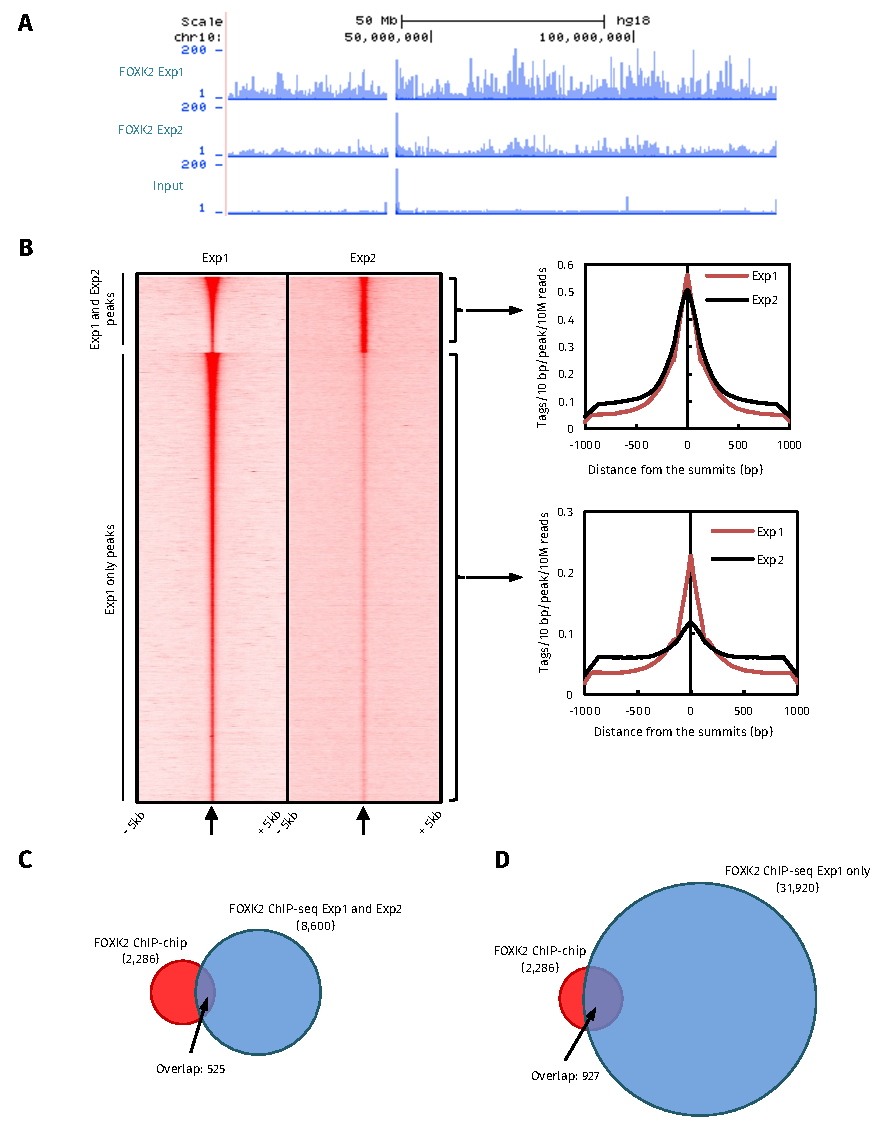
\includegraphics[width=0.9\textwidth]{chapter3/figures_overview/fig9.pdf}
    \caption[An overview of FOXK2 ChIP-seq data]{\textbf{An overview of FOXK2 ChIP-seq data. (A)} A snapshot of peak profiles of FOXK2 on the entire chromosome 10. Two ChIP experiments (indicated as Exp1 and Exp2) and one Input control are shown. \textbf{(B) Left,} heatmap of tag density profiles of the two FOXK2 ChIP-seq experiments around peaks that were identified from both experiments (Exp1 and Exp2 peaks), and peaks that were only identified from the first experiment (Exp1 only peaks). Tags were calculated in every 50 bp bin, and the density profiles were normalised to tags per 10 million total reads per bin. The middle point of each panel (indicated by small arrows below) represents the summit of the peak. 5 kb upstream and 5 kb downstream around the summit were plotted. \textbf{Right,} quantification of average of tags around the summit of Exp1 and Exp2 peaks and Exp1 only peaks. Peaks were aligned by their summits, and a region of -1 and +1 kb relative to the summit was selected. Tags were calculated in every 10 bp bin and normalised to tags per 10 million total reads per bin per peak. (\textbf{C} and \textbf{D}) Venn diagrams representing the overlaps in binding regions occupied by FOXK2 in ChIP-chip and ChIP-seq experiments. 8,600 Exp1and Exp2 peaks are shown in (\textbf{C}) and 31,920 peaks identified in the first experiment are shown in (\textbf{D}).}
    \label{fig:fig9}
\end{figure}

In order to investigate the \textit{in vivo} binding specificity of FOXM1, FOXO3 and FOXK2, it is necessary to interrogate the genome-wide binding profiles of the three Forkhead transcription factors. The ChIP-seq analysis of FOXK2 has already been done in proliferating U2OS cells by Dr. Zongling Ji in the Sharrocks lab (\cite{ji2012the}). Two independent experiments were performed, and 8,600 peaks were identified as present in both experiments. However, when comparing these two experiments, the first experiment turned out to be more sensitive than the second one based on the number of peaks detected, the peak height of the signal profile (for an example on chromosome 10, see \textbf{Figure \ref{fig:fig9}A}), and the average of signal intensity around the peaks (\textbf{Figure \ref{fig:fig9}B}). Previously, a ChIP-chip experiment of FOXK2 was also performed on Affymetrix Human Promoter 1.0R arrays. A total of 2,286 enriched binding regions were identified, and 525 (23\%) of them overlap with the 8,600 FOXK2 ChIP-seq peaks. When comparing to the first ChIP-seq experiment, the overlap of the ChIP-chip data increased to 927 (41\%) (\textbf{Figure \ref{fig:fig9}C}) (\cite{ji2012the}). In addition, some ChIP-qPCR validation also indicated that a lot of binding sites that only existed in the first experiment were true (\textbf{data not shown}). Therefore, in order to capture more FOXK2 binding events, we focused on the first FOXK2 ChIP-seq experiment in this study. In addition, to extract high confidence peaks from only one experiment, two peak callers MACS (\cite{zhang2008model-based}) and HOMER (\cite{heinz2010simple}) were used to call peaks. Only peaks that were called by both programs were kept. In this way, a total of 31,920 FOXK2 peaks were identified.

To investigate whether U2OS cells are suitable for studying the genome-wide binding events of FOXM1 and FOXO3, the expression of FOXM1 and FOXO3 were examined in this cell line. Early studies showed that protein levels of many cell cycle regulators (\textit{e.g.} several cyclins) undergo dramatic changes in different cell cycle stages (\cite{hochegger2008cyclin-dependent}). Since FOXM1 and FOXO3 have been linked to cell cycle regulation (\cite{alvarez2001forkhead,laoukili2005foxm1}), we first checked whether their protein levels were regulated during cell cycle. U2OS cells were synchronised at G1/S boundary by double thymidine block, and the cell lysates were collected at different time points after release from the block, followed by flow cytometry analysis for cell cycle profile or western blot analysis for protein expression. Two major bands and multiple closely-positioned bands with different mobility were observed after probing with a FOXM1 antibody and a FOXO3 antibody, respectively (\textbf{Figure \ref{fig:fig10}A}). To determine which bands corresponded to FOXM1 and FOXO3 protein rather than non-specific binding of the antibodies to other proteins, western blot analyses were performed after the transfection of a non-targeting control siRNA and siRNAs against either \textit{FOXM1} or \textit{FOXO3}. In the case of FOXM1, the two major bands disappeared after the knockdown, indicating that both bands are FOXM1 protein (\textbf{Figure \ref{fig:fig10}B}, left panel). In the case of FOXO3, most bands were reduced to background level after knockdown except one upper band, indicating a non-specific band recognised by this antibody (\textbf{Figure \ref{fig:fig10}B}, right panel). After treating the cell lysate with lambda phosphatase, both FOXM1 and FOXO3 exhibited a single uniform motility band (data not shown and \cite{park2008anaphase-promoting}), which demonstrate that the differences of mobility of the proteins are due to phosphorylation.

The protein level of FOXO3 stayed relatively constant throughout the cell cycle (\textbf{Figure \ref{fig:fig10}A}, middle panel). However, both phosphorylation and expression of FOXM1 oscillated during the cell cycle, with a low level at G1 phase (\textbf{Figure \ref{fig:fig10}A}, lane 2) and the highest level as cells accumulate at G2 and M phase (\textbf{Figure \ref{fig:fig10}A}, lane 5).

\begin{figure}[h]
    \centering
    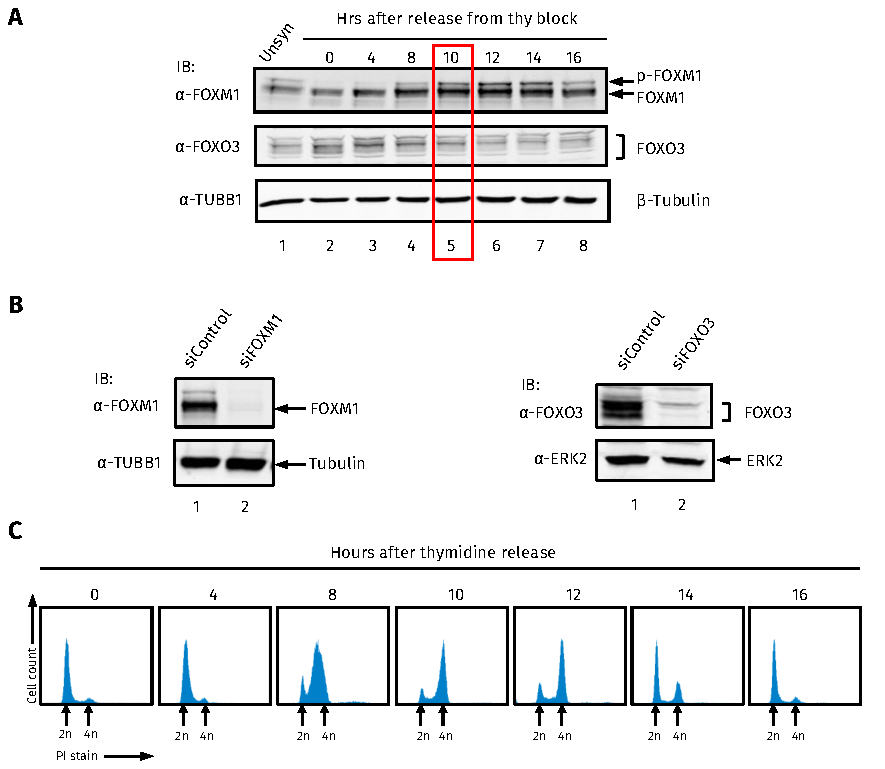
\includegraphics[width=0.9\textwidth]{chapter3/figures_overview/fig10.pdf}
    \caption[The expression of FOXM1 and FOXO3 in different cell cycle stages]{\textbf{The expression of FOXM1 and FOXO3 in different cell cycle stages. (A)} U2OS cell were synchronised at the G1/S boundary using double thymidine block and released into fresh media. Cells were collected at different time points as indicated after the release from double thymidine (thy) block. Total cell lysates were immunoblotted (IB) with the indicated antibodies to check the expression of endogenous FOXM1, FOXO3, and TUBB1 ($\beta$-Tubulin, as a loading control). Unsynchronised cells (Unsyn) are shown in lane 1. The positions of the bands corresponding to FOXM1/FOXO3 and the phosphorylated form of FOXM1 (p-FOXM1) are indicated. The red rectangle highlights the time point that was used for ChIP-seq experiments of FOXM1. \textbf{(B)} U2OS cells were transfected with a non-targeting control siRNA and siRNAs against either \textit{FOXM1} or \textit{FOXO3}. 48 hours after transfection, cell lysates were collected and immunoblotted with the indicated antibodies. TUBB1 and ERK2 were used as loading controls. \textbf{(C)} Flow cytometry analyses of the DNA content by propidium iodide (PI) staining of U2OS cells at different time points after the release from double thymidine block. The DNA content of diploid cells (2n) and tetraploid cells (4n) are indicated.}
    \label{fig:fig10}
\end{figure}

It is generally believed that protein abundance is an important factor that will influence ChIP-seq results (\cite{kidder2011chip-seq:}). Therefore, in order to maximise the chance of identifying the binding events, FOXM1 ChIP-seq analysis was performed in U2OS cells which were in the G2 and M phases of the cell cycle, \textit{i.e.} 10 hours after release from a double thymidine block (\textbf{Figure \ref{fig:fig10}A}, lane 5 and \textbf{Figure \ref{fig:fig10}C}), using a FOXM1 antibody.

\begin{figure}[!h]
    \centering
    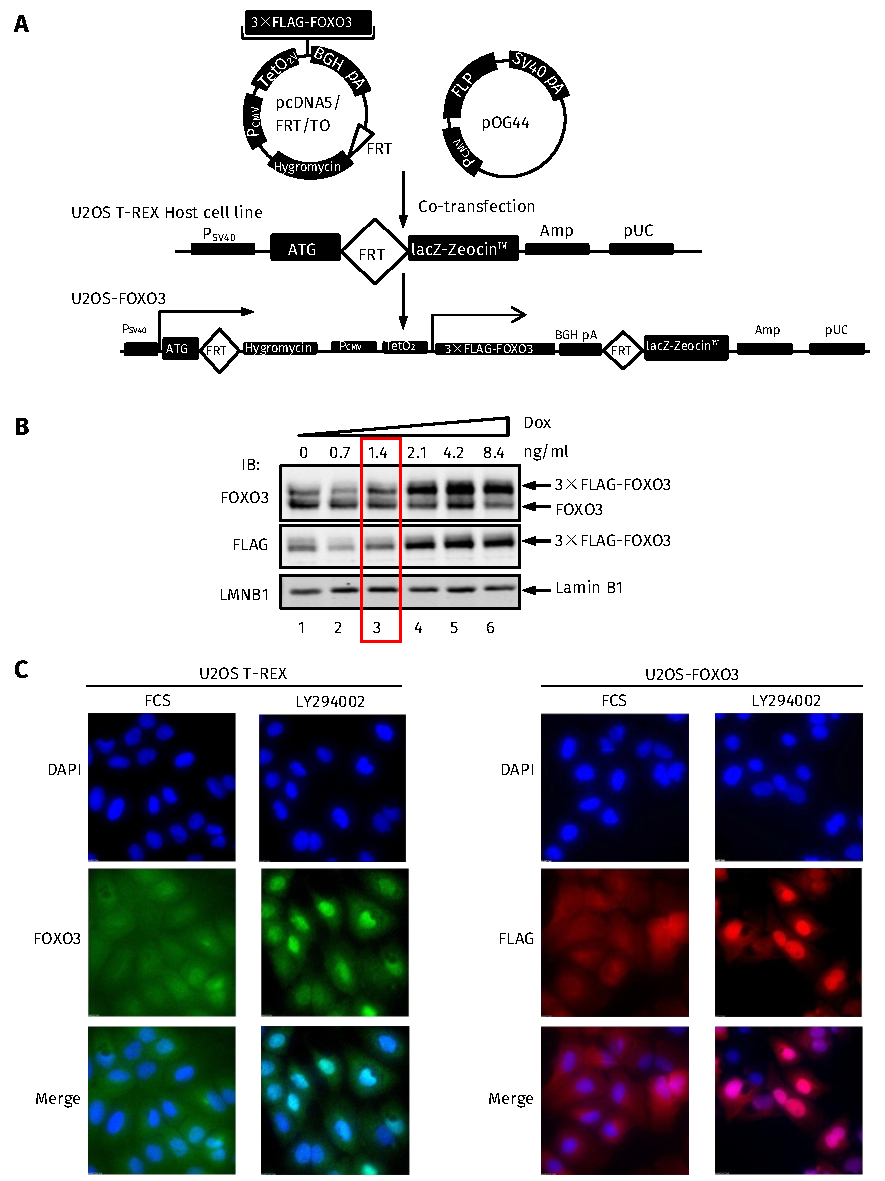
\includegraphics[width=0.9\textwidth]{chapter3/figures_overview/fig11.pdf}
    \caption[Establishment of 3$\times$FLAG-FOXO3 stable cell line]{\textbf{Establishment of 3$\times$FLAG-FOXO3 stable cell line. (A)} Schematic view of the strategy for constructing the 3$\times$FLAG-FOXO3 plasmid and the U2OS-FOXO3 stable cell line. \textbf{(B)} Varying concentrations of doxycycline (Dox) were added to culture media to induce the expression of the transgene. 24 hours after treatment, protein expression was examined by immunoblotting with different antibodies as indicated. LMNB1 (Lamin B1) was used as loading control. The positions of endogenous FOXO3 and 3$\times$FLAG-FOXO3 were indicated. The red rectangle indicates the concentration of doxycycline used for treating cells prior to ChIP. \textbf{(C)} Immunofluorescence analysis of endogenous FOXO3 and 3$\times$FLAG-FOXO3 cellular localisation in the U2OS T-REX host cell line and U2OS-FOXO3 stable cell line, respectively. The U2OS T-REX host cell line was stained with FOXO3 (75D8) antibody (\textit{i.e.} endogenous FOXO3; green) and DAPI; The U2OS-FOXO3 stable cell line was stained with FLAG antibody (\textit{i.e.} 3$\times$FLAG-FOXO3; red) and DAPI. Where indicated, cells were treated with 20 $\mu$M LY294002 or maintained in media containing FCS without this inhibitor.}
    \label{fig:fig11}
\end{figure}

Due to the lack of a suitable ChIP-grade antibody for FOXO3, a triple FLAG epitope tag was introduced to the N-terminus of FOXO3 (3$\times$FLAG-FOXO3) and cloned into the pcDNA5/FRT/TO vector (\textbf{Figure \ref{fig:fig11}A}). In this vector, the expression of 3$\times$FLAG-FOXO3 is driven by a tetracycline-inducible CMV promoter. The pcDNA5/FRT/TO/3$\times$FLAG-FOXO3 construct was co-transfected with the pOG44 vector, which encodes the Flp recombinase, into the Flip-In\sus{TM} U2OS host cell line that stably expresses the Tet repressor and contains a single integrated FRT site. After the co-transfection, the stable cell line (U2OS-FOXO3) was generated by maintaining the cells in the appropriate selection markers. By this approach, the U2OS-FOXO3 stable cell line was obtained which has only one single copy of the 3$\times$FLAG-FOXO3 transgene integrated into the specific locus in the genome, and the expression of the transgene can be controlled by adding varying concentrations of tetracycline/doxycycline (\textbf{Figure \ref{fig:fig11}A}). To examine the expression of 3$\times$FLAG-FOXO3 in response to doxycycline, different amounts of doxycycline were added to induce the expression of the transgene for 24 hours (18 hours after induction, the expression of 3$\times$FLAG-FOXO3 already became saturated, data not shown). Under normal cell culture condition (\textit{i.e.} DMEM with 10\% FCS) and without adding any doxycycline, there was some basal expression of 3$\times$FLAG-FOXO3 (\enquote{leaky} expression) due to the presence of tetracycline in the FCS (\textbf{Figure \ref{fig:fig11}B}, lane 1). The expression of 3$\times$FLAG-FOXO3 went up in line with the increase of the concentration of doxycycline added, and its level reached saturation when the concentration of doxycycline was at 4.2 ng/mL (\textbf{Figure \ref{fig:fig11}B}, lane 5).

Previous studies have shown that the nuclear localisation of FOXO3 is tightly controlled by PI3K/AKT signalling. Phosphorylation of FOXO3 by AKT results in its nuclear export through the interaction with 14-3-3 protein, and inhibition of PI3K/AKT signalling causes FOXO3 to enter the nucleus (\cite{brunet1999akt}). To check that the epitope-tagged FOXO3 behaves in the same way as the endogenous FOXO3, the localisation of the 3$\times$FLAG-FOXO3 was examined by immunofluorescence with or without LY294002, a specific inhibitor of PI3 kinase. As expected, under normal cell culture condition (in the presence of FCS), the endogenous FOXO3 is dispersed throughout the cytoplasm and the nucleus. After treatment with LY294002, most FOXO3 was relocated into the nucleus (\textbf{Figure \ref{fig:fig11}C}, left panel). Similarly, 3$\times$FLAG-FOXO3 spread out between the cytoplasm and the nucleus in the presence of FCS, and was predominantly located in the nucleus after addition of LY294002 (\textbf{Figure \ref{fig:fig11}C}, right panel). This demonstrates that the FLAG tagged FOXO3 transgene behaves in a similar manner to endogenous FOXO3.

Therefore, to investigate the genome-wide binding events of FOXO3, doxycycline was added at a concentration of 1.4 ng/mL which induced 3$\times$FLAG-FOXO3 expression to a level that is comparable to the endogenous FOXO3 (\textbf{Figure \ref{fig:fig11}B}, lane 3). A ChIP-seq experiment was performed under these conditions on U2OS-FOXO3 stable cell line using a FLAG antibody after 24 hours treatment with LY294002. In the meantime, a control ChIP experiment was also performed on U2OS T-REX host cell line which does not express the 3$\times$FLAG-FOXO3 transgene using the same antibody.

In summary, both FOXM1 and FOXO3 are expressed in U2OS cells, indicating this cell line is suitable for studying the genome-wide binding events of these two factors. The strategies for performing ChIP-seq experiments for FOXM1 and FOXO3 have been successfully established.

\subsection{Genome-wide chromatin-binding landscapes of Forkhead transcription factors}

Two biological replicates were performed for FOXM1 ChIP-seq experiments, yielding 27,892,797 and 8,906,067 uniquely mapped reads. MACS was used to call peaks, and a total of 270 peaks which were called from both experiments were identified as high confidence FOXM1 peaks. Although the sequencing depth of the second replicate was lower than the first one, the average peak signals of the second experiment was higher than the first one (\textbf{Figure \ref{fig:fig12}A}). In addition, quantitative comparison between the signal intensities from the two replicates showed that the two experiments have good correlation ($r=0.82$, Pearson correlation coefficient) (\textbf{Figure \ref{fig:fig12}B}), suggesting that the qualities of the two replicates around these peaks were similar.

Only one experiment was performed for FOXO3 ChIP-seq, yielding 38,149,670 mappable reads. In order to get high confidence peaks from one experiment, the same method which was used to extract FOXK2 peaks was applied to the FOXO3 ChIP-seq data. By the use of MACS and HOMER, a total of 6,089 peaks which were called by both programs were preserved as high confidence FOXO3 peaks.

The numbers of binding sites were vastly different among these three factors. This became apparent by looking at the peak profile across chromosomes as illustrated from the chromosome 1 (\textbf{Figure \ref{fig:fig13}A} and \textbf{B}). In particular, the small number of FOXM1 peaks is significantly less than commonly-observed number of peaks for other human transcription factors in cell culture systems (reviewed in \cite{macquarrie2011genome-wide}).

\begin{figure}[!h]
    \centering
    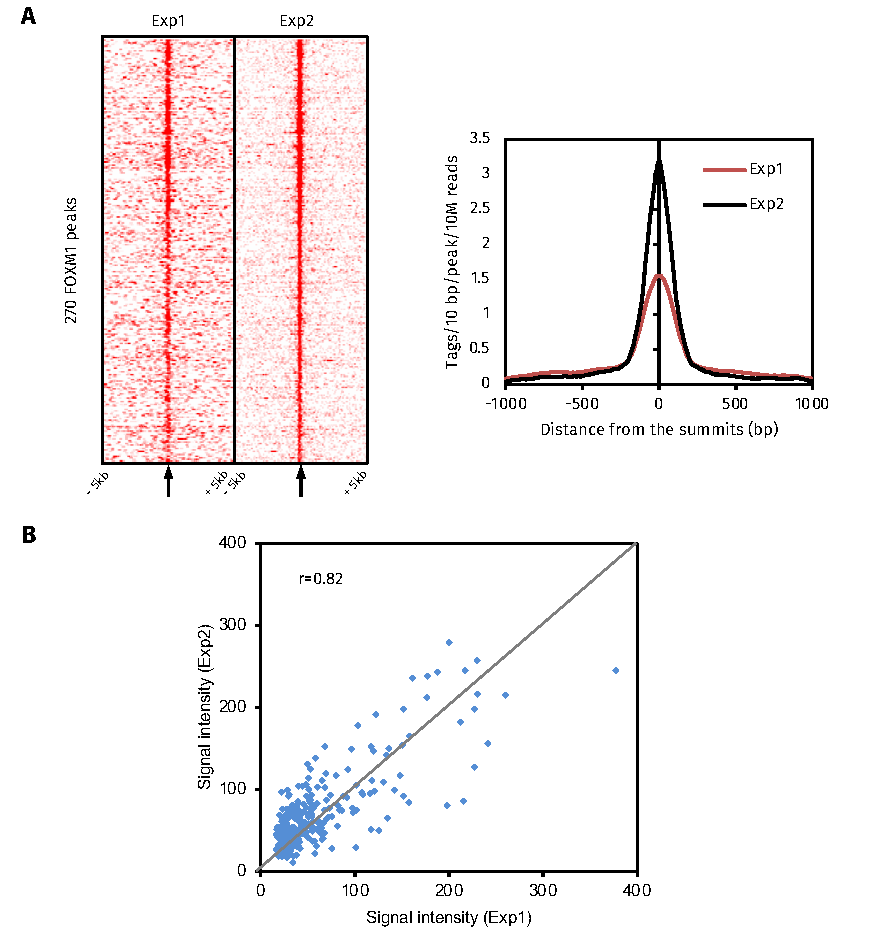
\includegraphics[width=0.9\textwidth]{chapter3/figures_overview/fig12.pdf}
    \caption[Comparison of the two replicates of FOXM1 ChIP-seq experiment]{\textbf{Comparison of the two replicates of FOXM1 ChIP-seq experiment. (A) Left,} heatmap of tag density profiles of the two replicates of FOXM1 ChIP-seq experiments around peaks that were identified from both replicates. Tags were calculated in every 50 bp bin, and the density profiles were normalised to tags per 10 million total reads per bin. The middle point of each panel (indicated by small arrows below) represents the summit of the peak. 5 kb upstream and 5 kb downstream around the summit were plotted. \textbf{Right,} quantification of average of tags around the summit of peaks. Peaks were aligned by their summits, and a region of -1 and +1 kb relative to the summit was selected. Tags were calculated in every 10 bp bin and normalised to tags per 10 million total reads per bin per peak. \textbf{(B)} Quantitative comparison of signal intensities of the two replicates of FOXM1 ChIP-seq experiments across 1-kb bins around the peaks. $r$, Pearson correlation coefficient.}
    \label{fig:fig12}
\end{figure}

Different transcription factors have different tendencies to bind to promoters, enhancers or gene bodies (reviewed in \cite{macquarrie2011genome-wide}). To find out whether FOXM1, FOXO3 and FOXK2 have similar tendencies to bind to the genomic regions, the distributions of FOXM1, FOXO3 and FOXK2 relative to the annotated transcription start sites (TSS) were analysed by the \textit{cis}-regulatory element annotation system (CEAS) (\cite{shin2009ceas:}). The genomic distributions of their peaks varied greatly. Here we define promoters as regions that are from the 5'-UTR to 1 kb upstream of the TSS. FOXM1 tends to bind promoter regions, with 73.7\% of its peaks in promoters (\textbf{Figure \ref{fig:fig13}B}), and FOXM1 peaks are significantly depleted at distal intergenic and intronic regions comparing to the genome background ($P$-values: $5.85 \times 10^{-21}$ and $1.09 \times 10^{-14}$, respectively, Fisher’s exact tests). This pattern of distribution is similar to transcription factors like ELK1 which also tends to bind proximal promoter regions (\cite{odrowaz2012elk1}). The distributions of FOXO3 and FOXK2 peaks were nearly identical, and they were in stark contrast to that of FOXM1 peaks. Only a small proportion (\textasciitilde 5\%) of FOXO3 and FOXK2 peaks reside in promoters, although this proportion is still more than the genome background (\textbf{Figure \ref{fig:fig13}B}). The majority of the peaks of both factors are located in distal intergenic and intronic regions, suggesting potential enhancer binding activity of these two factors (\textbf{Figure \ref{fig:fig13}B}). This is very similar to many other transcription factors like GATA-2 (\cite{linnemann2011genetic}), and other Forkhead transcription factors like FOXA1 (\cite{hurtado2011foxa1}), but varies from FOXM1 and ELK1.

\begin{figure}[!h]
    \centering
    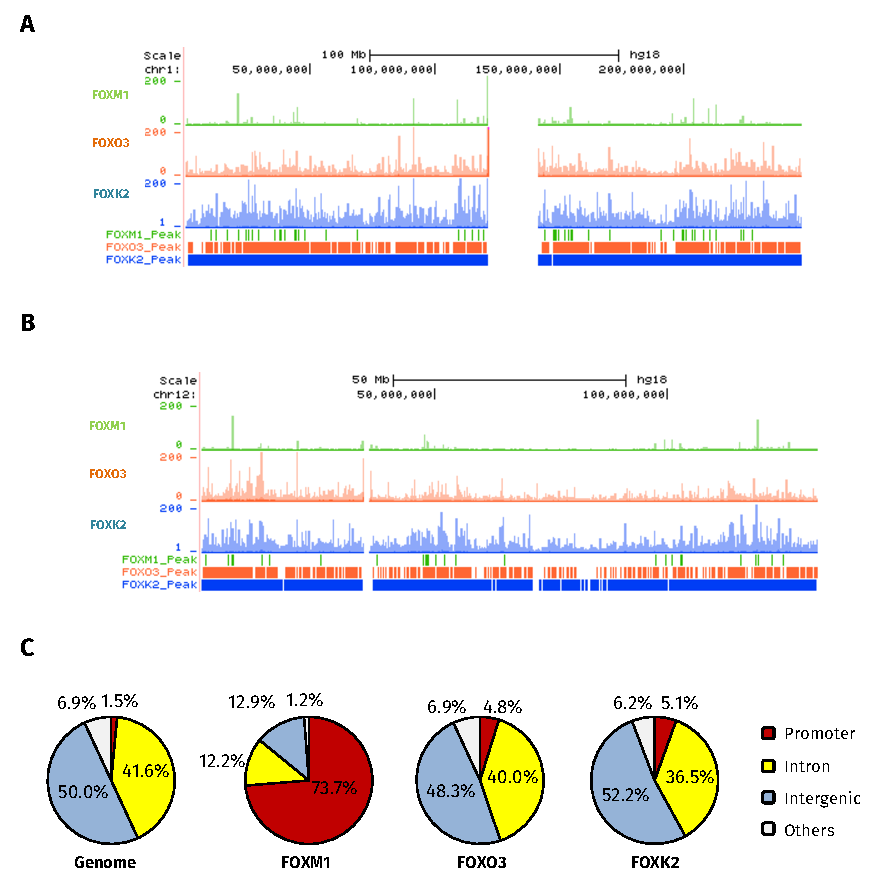
\includegraphics[width=0.9\textwidth]{chapter3/figures_overview/fig13.pdf}
    \caption[Examples of FOXM1, FOXO3 and FOXK2 ChIP-seq peaks]{\textbf{Examples of FOXM1, FOXO3 and FOXK2 ChIP-seq peaks. (A and B)} Two snapshots of all peaks for FOXM1, FOXO3 and FOXK2 on the entire chromosome 1 and 12. Locations of the peaks are indicated as bars (green for FOXM1, orange for FOXO3, and blue for FOXK2) below the peak profiles. Peak profiles on chromosome 1 is shown in \textbf{(A)}; peak profiles on chromosome 12 is shown in \textbf{(B)}. \textbf{(C)} The genomic distributions of the binding peaks for FOXM1, FOXO3 and FOXK2. Analyses were performed using \textit{cis}-regulatory element annotation system (CEAS). The promoter was defined as regions of 1 kb upstream from a transcription start site and the 5'-UTR. The distal intergenic region was defined as regions located 3 kb away from a gene body. Others were defined as regions including coding exon, 3'-UTR and up to 3 kb downstream from a transcription termination site. The distribution of genomic DNA is shown on the left.}
    \label{fig:fig13}
\end{figure}

Factors from the same family tend to have both redundant and specific binding events, due to their conserved DNA-binding domain. To investigate whether this is the case within FOXM1, FOXO3 and FOXK2, pairwise comparison of the peaks from the three Forkhead transcription factors were performed. Similar to members from other families, they had both overlapping and specific binding events (\textbf{Figure \ref{fig:fig14}A} and \textbf{B}). However, the extent of overlap among their peaks differed greatly. Here we define the overlapping peak as one where peaks share at least one base pair.

\begin{figure}[!h]
    \centering
    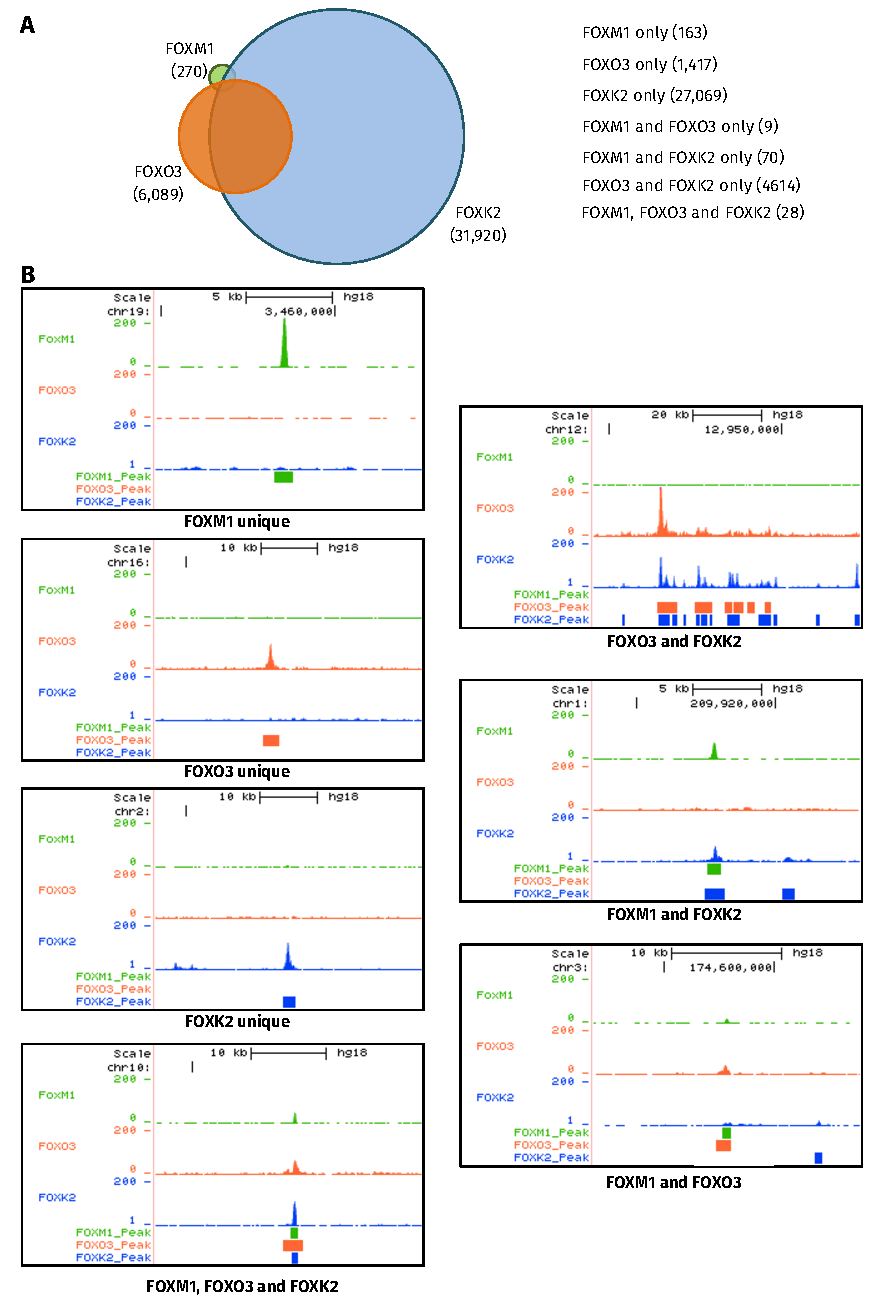
\includegraphics[width=0.8\textwidth]{chapter3/figures_overview/fig14.pdf}
    \caption[Examples of specific and overlapping binding events of FOXM1, FOXO3 and FOXK2]{\textbf{Examples of specific and overlapping binding events of FOXM1, FOXO3 and FOXK2. (A)} Venn diagram shows the overlap of the binding peaks for FOXM1, FOXO3 and FOXK2. \textbf{(B)} Snapshots showing examples of FOXM1, FOXO3 and FOXK2 peaks. Both unique and redundant peaks are shown.}
    \label{fig:fig14}
\end{figure}

Since FOXK2 had significantly more peaks than the other two factors, it also had many specific peaks of its own. However, the majority of FOXO3 peaks were shared with FOXK2 (\textbf{Figure \ref{fig:fig14}A}). Based on previous functional studies on FOXK2 and FOXO3 which suggest they have quite different biological functions (\cite{brunet1999akt,marais2010cell,ji2012the}), such a great level of overlap between FOXO3 and FOXK2 peaks is quite unexpected. For a more detailed analysis and discussion, see \textbf{Section \ref{section:foxo3}}).

Only 38 peaks were bound by both FOXM1 and FOXO3, and the FOXO3 binding signals around these 38 peaks were very low comparing to FOXM1, indicating the low occupancy of FOXO3 at these 38 peaks (\textbf{Figure \ref{fig:fig15}A}, left and middle panels). Furthermore, the FOXO3 binding signal was not located near the summits of FOXM1 peaks (\textbf{Figure \ref{fig:fig15}A}, left panel). In addition, when comparing the binding signals to the overall FOXO3 binding, it turned out that the FOXO3 binding at these 38 peaks were not as good as overall FOXO3 binding (\textbf{Figure \ref{fig:fig15}A}, right panel). Therefore, FOXM1 and FOXO3 do not seem to bind to the exact same regions.

There were 98 peaks shared by both FOXM1 and FOXK2. Although FOXK2 had decent binding signals around these 98 peaks, they were still very low compared to FOXM1 (\textbf{Figure \ref{fig:fig15}B}, left and middle panels). However, when comparing to the FOXK2 overall binding, the FOXK2 binding within these 98 peaks were comparable to its overall average binding signals (\textbf{Figure \ref{fig:fig15}B}, right panel). Indeed, we did observe higher signal intensities of FOXK2 in these 98 peaks comparing to the overall FOXK2 binding (\textbf{Figure \ref{fig:fig15}B}, right panel), but the background signals at these 98 peaks were also higher than the overall background, probably because most of these 98 peaks are located in core promoter regions which tend to get more reads in ChIP-seq experiments (\cite{auerbach2009mapping,cheung2011systematic}). In addition, the FOXK2 binding signals were also very close to the summits of FOXM1 peaks (\textbf{Figure \ref{fig:fig15}B}, right panel). Therefore, the position and the intensity of the FOXK2 signal profiles around these 98 peaks indicate that they represent binding regions for both FOXM1 and FOXK2.

\begin{figure}[!ht]
    \centering
    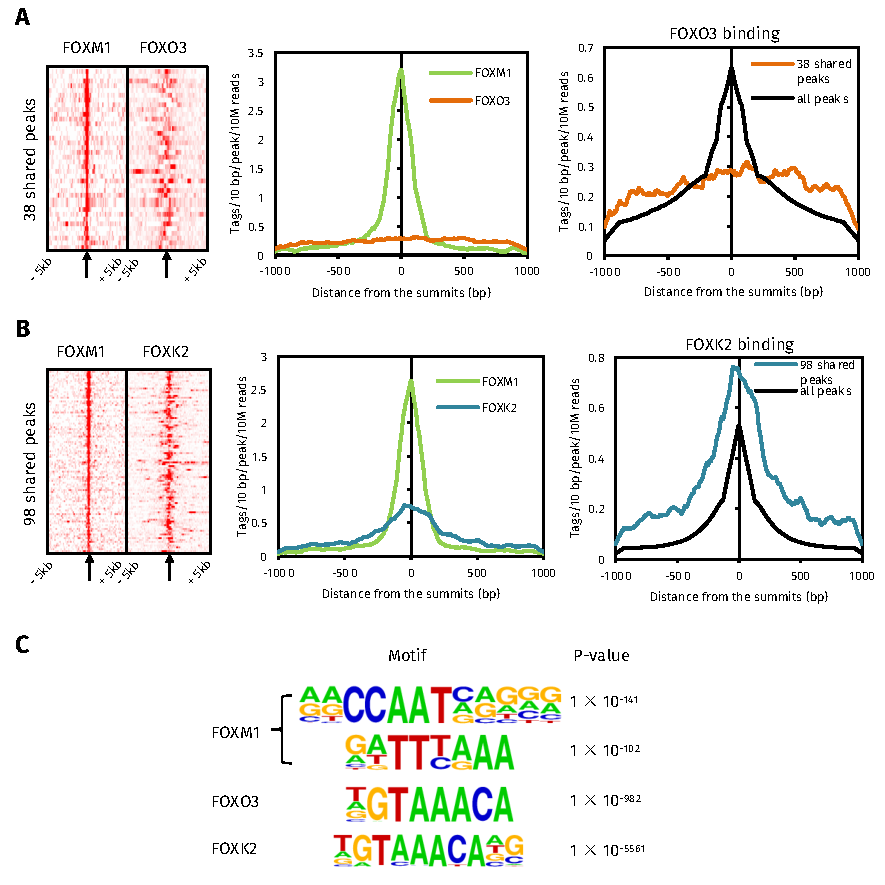
\includegraphics[width=0.8\textwidth]{chapter3/figures_overview/fig15.pdf}
    \caption[Comparisons of genome-wide binding events of Forkhead transcription factors]{\textbf{Comparisons of genome-wide binding events of Forkhead transcription factors. (A) Left,} heatmap of tag density profiles of FOXM1 and FOXO3 around the 38 peaks that are bound by both FOXM1 and FOXO3. Tags were calculated in every 50 bp bin, and the density profiles were normalised to tags per 10 million total reads per bin. The middle point of each panel (indicated by small arrows below) represents the summit of the FOXM1 peak. 5 kb upstream and 5 kb downstream around the summit were plotted. \textbf{Middle,} quantification of average of tags of FOXM1 and FOXO3 around the summit of the 38 peaks bound by both factors. Peaks were aligned by the FOXM1 summits, and a region of -1 and +1 kb relative to the summit was selected. Tags were calculated in every 10 bp bin and normalised to tags per 10 million total reads per bin per peak. \textbf{Right,} quantification of average of tags of FOXO3 on all FOXO3 peaks and the 38 peaks bound by FOXM1 and FOXO3. Tags were calculated in every 10 bp bin and normalised to tags per 10 million total reads per bin per peak. \textbf{(B)} The same analysis as \textbf{(A)} on the 98 peaks bound by both FOXM1 and FOXK2. \textbf{(C)} The top motifs returned by Homer \textit{de novo} motif discovery program from the 200 bp around the summits of ChIP-seq derived peaks for FOXM1, FOXO3 and FOXK2. The P-value was calculated based on hypergeometric distributions.}
    \label{fig:fig15}
\end{figure}

\textit{De novo} motif discovery is the most commonly-used method to find out the DNA sequence bound by a particular factor in the ChIP-seq study. The top motif returned by a motif discovery algorithm often reflects the DNA sequence bound by the factor \textit{in vivo}. To investigate the DNA sequences bound by these three Forkhead transcription factors, HOMER was used to perform \textit{de novo} motif discovery on the ChIP-seq data of FOXM1, FOXO3, and FOXK2. The most over-represented DNA sequence in the FOXM1 ChIP-seq peaks returned by HOMER were the CCAAT-box which is bound by the transcription factor NF-Y, and a motif that resembles the CHR (\underline{c}ell cycle \underline{h}omology \underline{r}egion) sequence (reviewed in \cite{müller2010the}). Surprisingly, the canonical Forkhead motif is not enriched in FOXM1 bound peaks (\textbf{Figure \ref{fig:fig15}C}). In contrast, the top DNA sequence motifs returned from the FOXK2 and FOXO3 ChIP-seq peaks were both canonical Forkhead motifs containing the core GTAAACA sequence (\textbf{Figure \ref{fig:fig15}C}).

In summary, FOXK2 has significantly more binding events than the other two Forkhead proteins. FOXO3 tends to bind redundantly with FOXK2, and only has a small proportion of specific peaks of its own. In contrast, FOXM1 seems to be an atypical Forkhead transcription factor and has its own specific binding event. This conclusion is based on its small number of peaks, its distinctive pattern of genomic distribution, the relatively low tag signals of FOXO3 or FOXK2 at peaks shared with FOXM1, and the completely different motifs enriched in its peaks.

\subsection{Summary}

Collectively, the data presented in this section provide a detailed description of the experimental strategies and general overviews of the ChIP-seq analyses of FOXM1, FOXO3 and FOXK2. The experiments are carefully designed in a factor-specific manner to obtain an optimal ChIP condition for each factor, and stringent criteria are used to get high confidence data. The initial comparison of the three ChIP-seq data sets reveals several surprising points.

The first surprising discovery is the number of binding sites of these three factors. The number of peaks identified for FOXK2, FOXO3, and FOXM1 varies greatly. FOXK2 and FOXO3 have a comparable number of binding events to other transcription factors. However, FOXM1 only possesses a small number of binding sites, which is significantly less than the number of peaks for other human transcription factors. This difference becomes even more conspicuous when comparing FOXM1 to other Forkhead transcription factors, which are generally believed to have a lot of binding sites \textit{in vivo} (\textbf{Table \ref{table:fkhtfschip}}).

\begin{longtable}{|c|c|c|c|}
    %% table setup %%
    \caption{Comparison of number of binding sites for different Forkhead TFs\label{table:fkhtfschip}}\\
    \hline
    \textbf{Forkhead Protein} & \textbf{Cell line} & \textbf{\# of binding sites} & \textbf{Reference}\\
    \hline
    \endfirsthead
    \multicolumn{3}{l}{\textbf{\textit{Table \ref{table:fkhtfschip}}} continued}\\
    \hline
    \textbf{Forkhead Protein} & \textbf{Cell line} & \textbf{\# of binding sites} & \textbf{Reference}\\
    \hline
    \endhead
    \hline
    \multicolumn{3}{l}{\textit{continued on the next page}}\\
    \endfoot
    \hline \hline
    \endlastfoot
    
    %% actual content %%
    FOXA1 & MCF7 & 79,651 & \cite{hurtado2011foxa1}\\
    \hline
    FOXA1 & T47D & 43,446 & \cite{hurtado2011foxa1}\\
    \hline
    FOXA1 & ZR75-1 & 80,327 & \cite{hurtado2011foxa1}\\
    \hline
    FOXA1 & HepG2 & 8,175 & \cite{motallebipour2009differential}\\
    \hline
    FOXA2 & HepG2 & 7,153 & \cite{motallebipour2009differential}\\
    \hline
    FOXA3 & HepG2 & 4,598 & \cite{motallebipour2009differential}\\
    \hline
    FOXH1 & H9 ESC & 9,702 & \cite{kim2011chromatin}\\
    \hline
    FOXK1 & HeLa & 4,329 & \cite{grant2012live-cell}\\
    \hline
    FOXK2 & U2OS & 31,920 & \cite{ji2012the}\\
    \hline
    \color{red} \textbf{FOXM1} & U2OS & \color{red} \textbf{270} & This study\\
    \hline
    FOXO3 & U2OS & 6,089 & This study\\
    \hline
    FOXP1 & H9 ESC & 3,400 & \cite{gabut2011an}\\
    \hline
    FOXP2 & PFSK-1 & 1,814 & ENCODE project\\
    \hline
    FOXP2 & SK-N-MC & 3,133 & ENCODE project\\
    \hline
    FOXP3 & MCF7 & 40,551 & \cite{katoh2011foxp3}\\
    \hline
\end{longtable}

The second surprising discovery is the genomic distribution of these three Forkhead transcription factors. The majority of both FOXO3 and FOXK2 peaks are located in the distal intergenic and intronic regions, and only a small proportion of their peaks reside in the promoter regions. This feature is commonly observed in other Forkhead transcription factors and indicates that FOXO3 and FOXK2 might be enhancer binding factors (\cite{wang2011reprogramming}).  However, most FOXM1 peaks are very close to the TSS and are depleted from the distal intergenic and intronic regions, which is in sharp contrast to FOXO3 and FOXK2 but similar to other transcription factors like ELK1 (\cite{odrowaz2012elk1}). This implies that the mechanism used by FOXM1 to regulate transcription is probably different from that used by FOXO3 and FOXK2.

The third, perhaps the most, surprising discovery is the enriched motifs within the peaks of these three factors. Forkhead-like responsive element containing the core GTAAACA and some motifs that resemble the binding sites of other transcription factors are enriched within the FOXO3 and FOXK2 peaks (see \textbf{Section \ref{section:foxo3}}), with the Forkhead motif being the most overrepresented motif in both cases. Only two motifs are found enriched within the FOXM1 peaks: one is the CCAAT-box motif which is bound by the transcription factor NF-Y; the other is the CHR motif which is bound by the DREAM and the MMB complexes. Furthermore, the Forkhead motif is not enriched within the FOXM1 cistrome.

Based on our preliminary analyses stated above, FOXM1 seems to somehow have its own specific binding events, while FOXO3 and FOXK2 are more like conventional members within the Forkhead family, which have both specific and overlapping binding sites. Therefore, in the following sections, we first analyse how FOXM1 obtains its own specific binding sites compared to other typical Forkhead transcription factors. Then FOXK2 and FOXO3 binding are compared to interrogate how they acquire their overlapping and specific binding events.
\section{FOXM1 controls G2-M gene expression through atypical chromatin binding mechanisms}

\subsection{Validation of FOXM1 ChIP-seq data}

The analysis of next generation sequencing (NGS) data is computationally and statistically challenging. Currently there are no benchmarks for data processing methods (read mapping, peak calling \textit{etc.}). Hence false positives/negatives are common problems in experiments, such as ChIP-seq, based on NGS technologies (reviewed in \cite{pepke2009computation}). To confirm the reliability of the FOXM1 ChIP-seq data, vigorous validations were carried out.

\begin{figure}[!h]
    \centering
    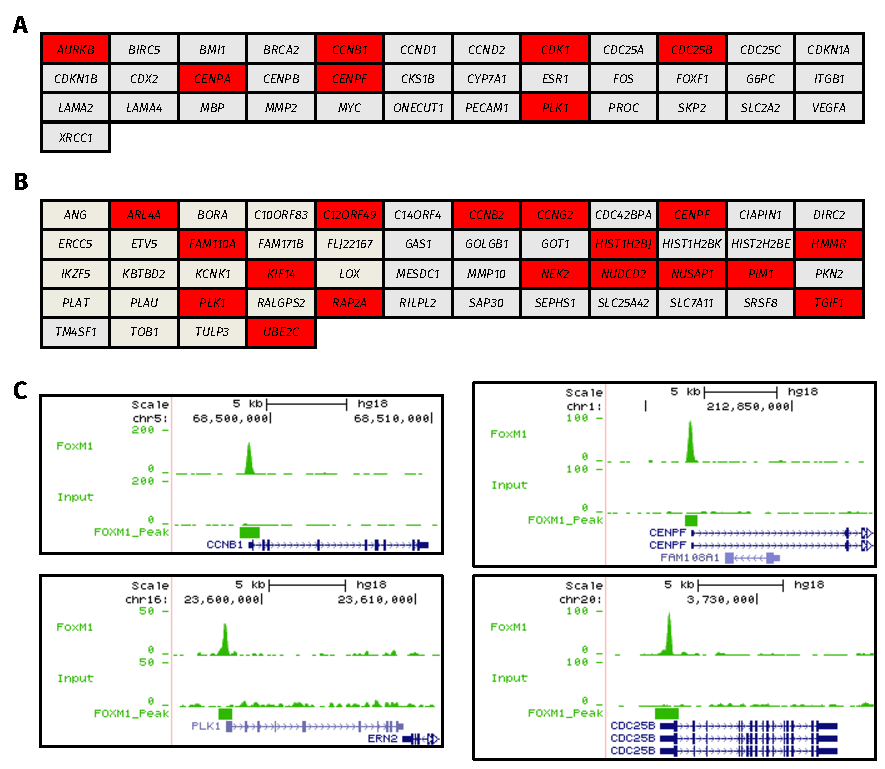
\includegraphics[width=0.9\textwidth]{chapter3/figures_foxm1/fig16.pdf}
    \caption[FOXM1 binding at known target genes]{\textbf{FOXM1 binding at known target genes. (A)} known target genes of FOXM1 according to The Transcription Factor Encyclopaedia (\cite{yusuf2012the}). Red colour indicates the genes that are also identified by the FOXM1 ChIP-seq experiment. \textbf{(B)} 52 FOXM1 target genes identified from the microarray analysis (\cite{laoukili2005foxm1}). \textbf{(C)} Snapshots of FOXM1 peak profile at the four well-known target genes.}
    \label{fig:fig16}
\end{figure}

Since many FOXM1 target genes have been discovered in the past, we first checked whether those known target genes were also identified by our FOXM1 ChIP-seq analysis. To this end, we looked into The Transcription Factor Encyclopaedia (\cite{yusuf2012the}), a manually-curated transcription factor database, and found 37 potential target genes of FOXM1 according to previous wet lab experimental evidence. 7 out of 37 genes were bound by FOXM1 based on our ChIP-seq data (\textbf{Figure \ref{fig:fig16}A}). In addition, an early study used microarray analysis and revealed 52 genes that were upregulated when FOXM1 was overexpressed in U2OS cells (\cite{laoukili2005foxm1}). 17 out of 52 genes were bound by FOXM1 (\textbf{Figure \ref{fig:fig16}B}). Note that the target genes from the database and the microarray analysis include both direct and indirect targets of FOXM1, while the genes identified from the ChIP-seq are more likely to be direct FOXM1 targets. In particular, the previously well-established FOXM1 targets \textit{CCNB1, CDC25B, CENPF} and \textit{PLK1} were all present in our FOXM1 ChIP-seq data (\textbf{Figure \ref{fig:fig16}C}) (\cite{laoukili2005foxm1,wang2005forkhead}).

Having confirmed that some known target genes were successfully identified by our FOXM1 ChIP-seq experiment, we next picked different peaks from the ChIP-seq data and used locus-specific ChIP-qPCR to validate the FOXM1 binding at these regions in U2OS cells. FOXM1 binding peaks were ranked by fold enrichment over $\lambda_{local}$, and thirteen peaks with different enrichments were selected. Eleven of these regions showed at least 4 fold enrichment over a non-specific IgG control (\textbf{Figure \ref{fig:fig17}A}).

To further confirm that the ChIP-seq derived peaks were genuine FOXM1 peaks, ChIP experiments were performed on U2OS cells using the FOXM1 antibody after transfection with siRNA against either GAPDH or FOXM1. The FOXM1 binding signal at three tested regions were significantly reduced after the FOXM1 knockdown (\textbf{Figure \ref{fig:fig17}B}), suggesting that the binding signals at those regions represented real FOXM1 binding.

Since the FOXM1 binding events identified from the ChIP-seq analysis were from cells which are at the G2 and M phases, we next checked whether FOXM1 binds to its target genes at other stages of the cell cycle. To this end, U2OS cells were synchronised at the G1/S boundary by a double thymidine block, and cells were released from the thymidine block to allow them to enter the cell cycle. Then FOXM1 ChIP experiments were performed when cells were accumulated at different cell cycle phases: 5 hours after the release (S phase) and 10 hours after the release (G2/M phase). The binding of FOXM1 to four tested target genes happened as early as the G1/S boundary (\textbf{Figure \ref{fig:fig17}C}, 0h time point). Interestingly, the binding of FOXM1 remained relatively constant throughout the different cell cycle stages (\textbf{Figure \ref{fig:fig17}C}), which is consistent with previous findings (\cite{laoukili2008activation}).

\begin{figure}[!h]
    \centering
    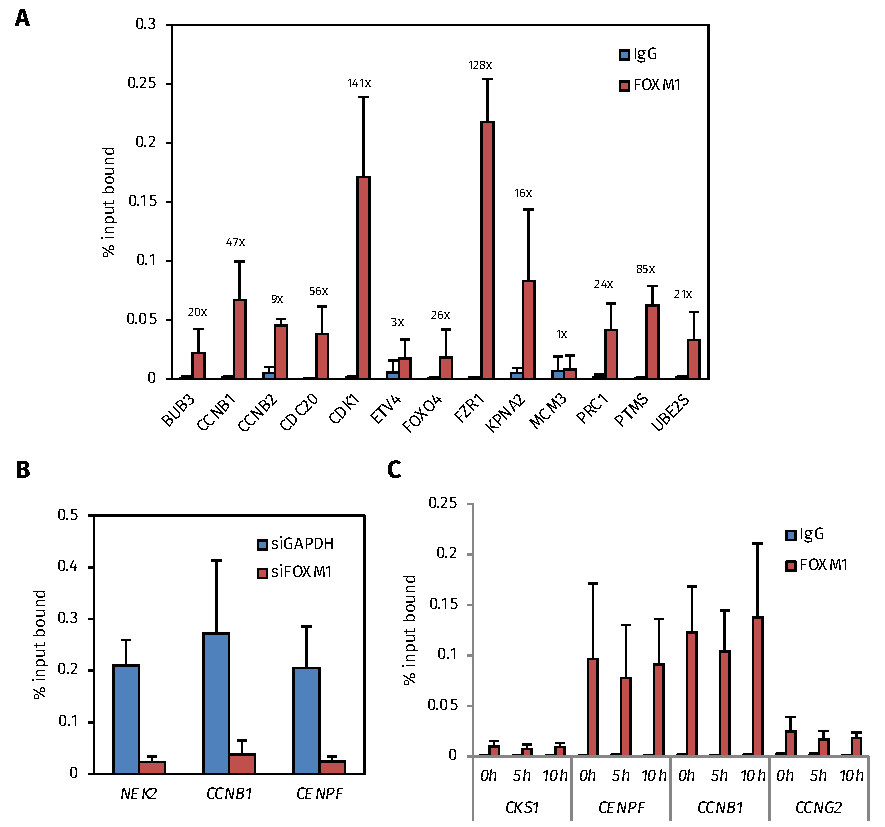
\includegraphics[width=0.9\textwidth]{chapter3/figures_foxm1/fig17.pdf}
    \caption[ChIP-qPCR validation on selected FOXM1 peaks]{\textbf{ChIP-qPCR validation on selected FOXM1 peaks. (A)} 13 randomly selected FOXM1 peaks were tested by ChIP-qPCR in U2OS cells using a FOXM1 antibody and a non-specific IgG control antibody. Fold enrichment over the IgG control is indicated above the bar. The error bars represent the standard deviations from three independent experiments. \textbf{(B)} Examination of FOXM1 binding by ChIP-qPCR on three FOXM1 peaks after FOXM1 knockdown. U2OS cells were transfected with 20 nM siRNA against either GAPDH or FOXM1, and cells were collected 48 hours after the transfection. ChIP experiments were performed using a FOXM1 antibody. The error bars represent the standard deviations from two independent experiments. \textbf{(C)} The promoter binding of FOXM1 at different cell cycle stages. U2OS cells were collected at the indicated time points after the release from a double thymidine block. ChIP experiments on the indicated loci were performed using a FOXM1 antibody. The error bars represent the standard deviations from either three independent experiments (the \textit{CKS1, CENPF} and \textit{CCNB1} loci) or two independent experiments (the \textit{CCNG2} locus).}
    \label{fig:fig17}
\end{figure}

In summary, our FOXM1 ChIP-seq data is consistent with previous findings about FOXM1. Most of the peaks validated from the ChIP-seq data have real FOXM1 binding. The binding of FOXM1 at a subset of tested regions happens at the early stages of the cell cycle and remain relatively constant during the cell cycle. These findings indicate that the quality of our FOXM1 ChIP-seq data is good.

\pagebreak

\subsection{FOXM1 regulates a large array of late cell cycle genes}

After confirming the reliability of the FOXM1 ChIP-seq data, the biological functions and the molecular mechanisms of FOXM1 binding were investigated.

FOXM1 is known as a cell cycle regulator, and it is required for proper G2-M transition and chromosome segregation (\cite{laoukili2005foxm1,wang2005forkhead}). To establish whether more of the FOXM1 target genes were also involved in G2-M cell cycle regulation and to discover potential novel functions of FOXM1, the ChIP-seq derived peaks were analysed by the \underline{G}enomic \underline{R}egions \underline{E}nrichment of \underline{A}nnotations \underline{T}ool (GREAT), an analytical tool of gene ontology (\cite{mclean2010great}). Previous gene ontology methods only take the proximal binding events into consideration, simply assign one binding event to its nearest gene, and use gene-based tools to perform the functional interpretation (\cite{huang2009bioinformatics}). Unlike the traditional methods, GREAT is a peak/region-based analysis, which is more similar to the nature of the transcription factor ChIP-seq data. In GREAT, each gene is first given a basal domain which is from 5 kb upstream to 1 kb downstream of the TSS of that gene. Then the basal domain is extended upstream and downstream to the basal domains of its neighbouring genes within 1 Mb. The resulting basal plus extension domain is denoted as the regulatory domain of the gene, and any peaks that fall into the regulatory domains will be assigned to the particular genes (\textbf{Figure \ref{fig:fig18}A}). Only enriched terms that satisfy both binomial and hypergeometric tests are returned. In this way, GREAT is able to associate a peak and its potential target genes together even if they are far away. This approach significantly improves the functional interpretation of the transcription factor binding events (\cite{mclean2010great}).

\begin{figure}[!h]
    \centering
    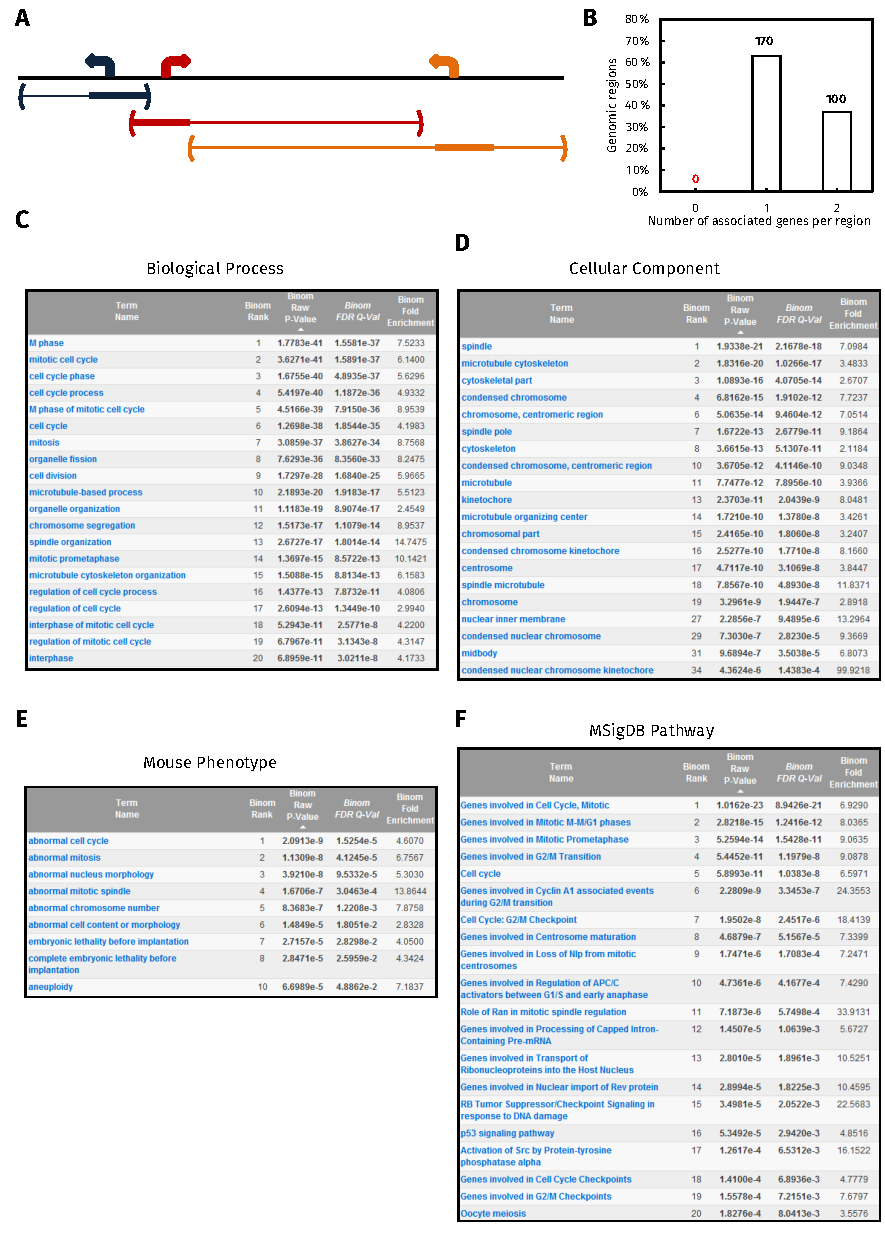
\includegraphics[width=0.9\textwidth]{chapter3/figures_foxm1/fig18.pdf}
    \caption[Gene ontology analysis of FOXM1 peaks by GREAT]{\textbf{Gene ontology analysis of FOXM1 peaks by GREAT. (A)} The basal plus extension rules of GREAT. The arrow indicates the transcription start site of each gene. The thick line and the thin line represent the basal (-5 kb plus +1 kb relative to the TSS) and the extended domain (up to 1 Mb) respectively. The whole regulatory domain for each gene is shown as a bracketed line in matched colour. \textbf{(B)} Histogram showing number of associated genes per peak. \textbf{(C, D, E and F)} Top 20 terms of Biological Process \textbf{(C)}, top 20 terms of Cellular Component \textbf{(D)}, all terms of Mouse Phenotype \textbf{(E)}, and top 20 terms of MSigDB Pathway \textbf{(F)}. The P-value, FDR, and fold enrichment based on binomial distribution are also given.}
    \label{fig:fig18}
\end{figure}

By the use of GREAT, all FOXM1 peaks were assigned to at least one gene per peak, and 100 peaks were assigned to two genes per peak (\textbf{Figure \ref{fig:fig18}B}). GREAT returned 91 enriched terms for Biological Process, 33 for Cellular Component, 9 for Mouse Phenotype, and 35 for MSigDB Pathway (\textbf{Figure \ref{fig:fig18}C-F}). Consistent with the previous notion that FOXM1 regulates the G2-M cell cycle transition, the majority of the Biological Process terms were related to cell cycle, mitosis, and chromosome segregation (\textbf{Figure \ref{fig:fig18}C}). In addition, most enriched terms of Mouse Phenotype and MSigDB Pathway were also linked to M phase and cell cycle, and many enriched Cellular Component terms, such as spindle, kinetochore, and centrosome, were critical for mitosis (\textbf{Figure \ref{fig:fig18}C}). In addition, there were also a few enriched terms which were not directly linked to cell cycle, such as DNA packaging, DNA conformation change and free ubiquitin chain polymerisation, although the P-values were not as significant as those cell cycle related terms (\textbf{Figure \ref{fig:fig19}}). This indicates that FOXM1 might also play some regulatory roles in those processes. Interestingly, many genes within the non-cell cycle terms are also G2-M transition regulators, indicating that some terms which are not directly linked to cell cycle are the biological processes associated with the mitotic cell cycle.

\begin{figure}[!h]
    \centering
    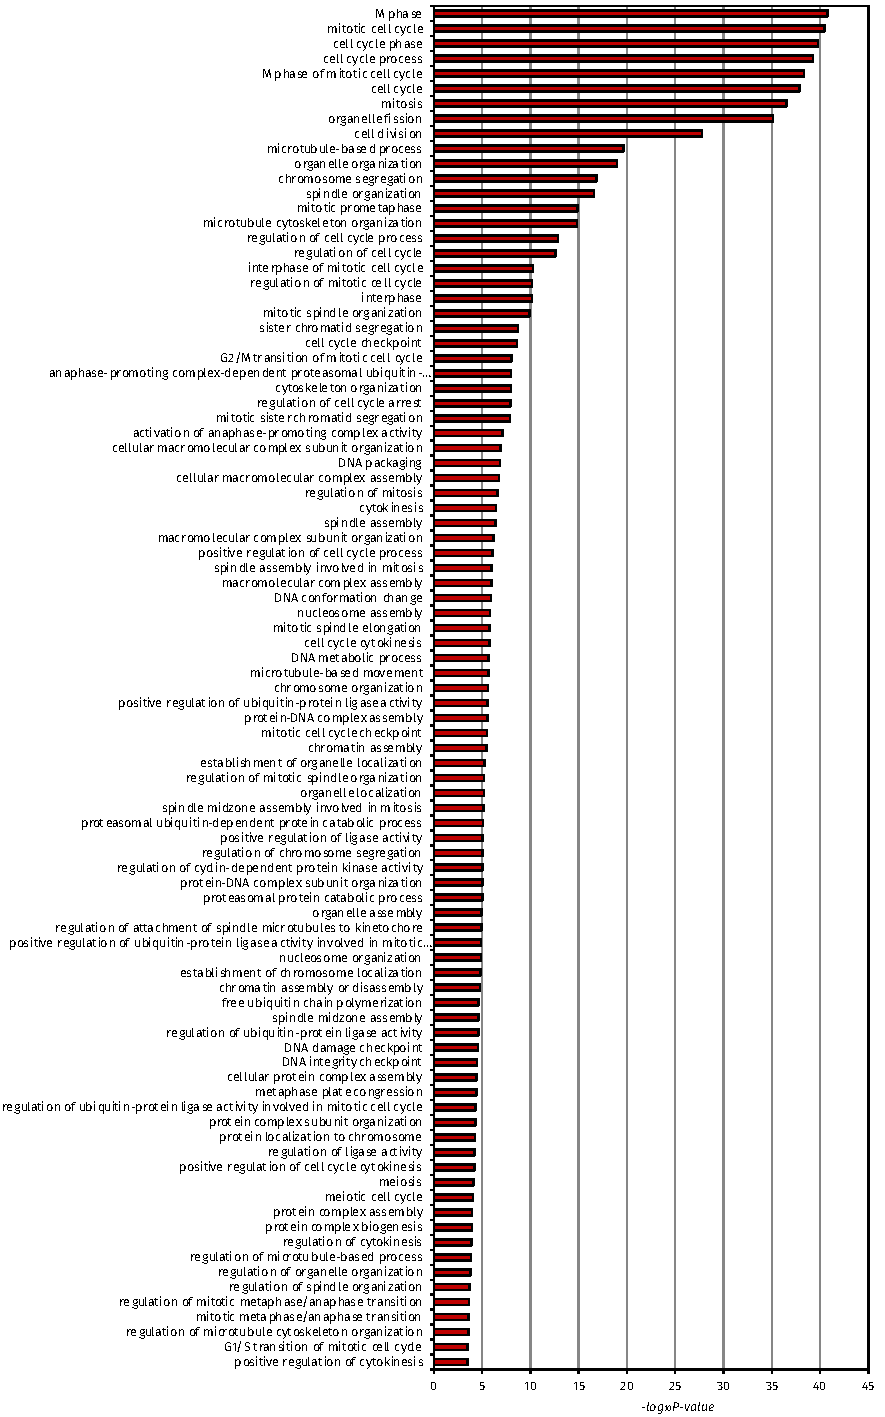
\includegraphics[width=0.8\textwidth]{chapter3/figures_foxm1/fig19.pdf}
    \caption[Enriched terms of Biological Process for FOXM1 peaks by GREAT]{\textbf{Enriched terms of Biological Process for FOXM1 peaks by GREAT.} An expansion of Figure 18C, showing all enriched terms from Biological Process which are sorted by -log\sub{10}P-value.}
    \label{fig:fig19}
\end{figure}

Given that most FOXM1 target genes were related to the cell cycle, especially mitosis, we then checked the expression patterns of all 362 FOXM1-bound genes assigned by GREAT throughout the cell cycle. To this end, we took advantage of a recent microarray study in HeLa cells after release from a double thymidine block, which examined the gene expression patterns in different cell cycle stages (\cite{sadasivam2012the}). Most of FOXM1-bound genes exhibited strong cell cycle-dependent expression, with peak activities when cells entered into G2 and M phase (\textbf{Figure \ref{fig:fig20}A}). This is consistent with the gene ontology analysis and suggests that FOXM1 has a role in controlling the temporal expression of genes in the G2 and M phases.

\begin{figure}[!h]
    \centering
    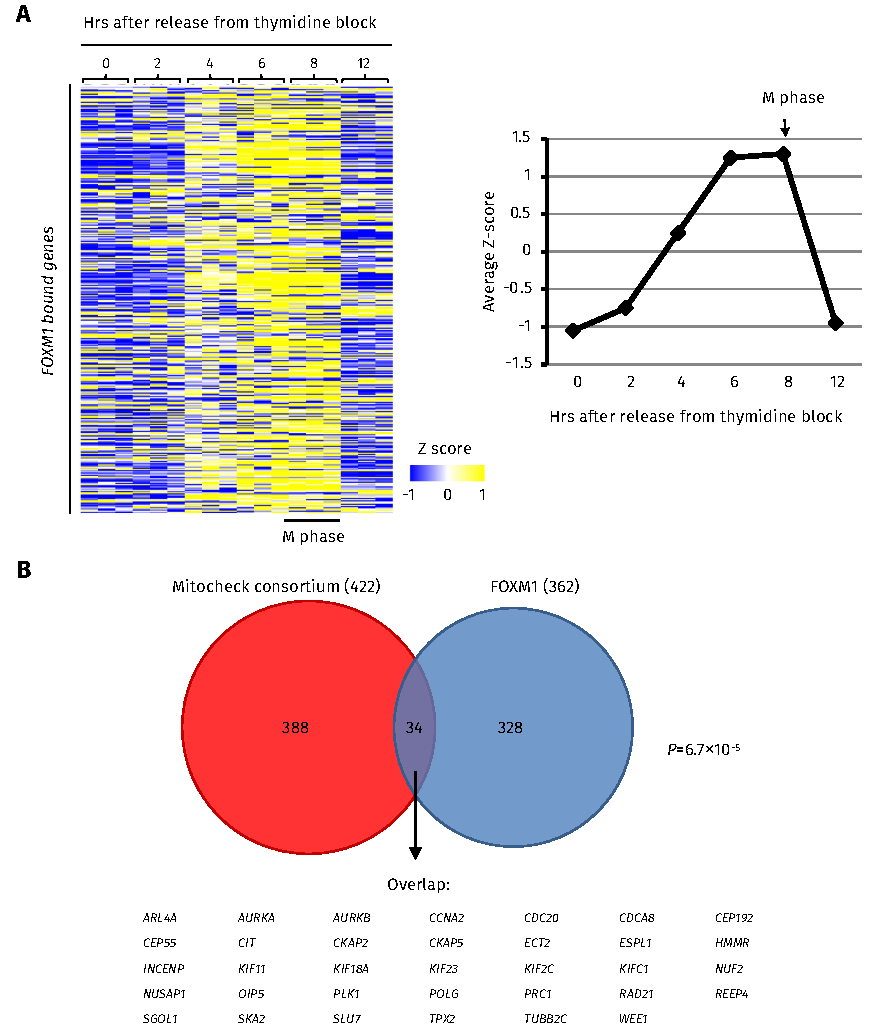
\includegraphics[width=0.9\textwidth]{chapter3/figures_foxm1/fig20.pdf}
    \caption[Expression patterns of FOXM1 bound genes throughout the cell cycle]{\textbf{Expression patterns of FOXM1 bound genes throughout the cell cycle. (A) Left,} heatmap of expression levels (represented by Z-score) of FOXM1 bound genes at the indicated time points after the release from a double thymidine block. The three replicates of each time point are shown. \textbf{Right,} average expression levels of FOXM1 bound genes at different cell cycle stages. This was done by Dr. Namshik Han. \textbf{(B)} Overlap between the 422 genes which give a mitotic phenotype when depleted (\cite{neumann2010phenotypic}) and 362 FOXM1 target genes assigned by GREAT. The overlapping genes are shown at the bottom. P-value was calculated by Fisher's exact test.}
    \label{fig:fig20}
\end{figure}

To further address the importance of FOXM1 in controlling late cell cycle events, we looked into the validation screen database of the Mitocheck consortium (\cite{neumann2010phenotypic}). This consortium carried out phenotypic profiling with a siRNA library targeting \textasciitilde 21,000 human protein coding genes using live-cell imaging. The validated database contained 422 genes which gave at least one mitotic phenotype upon knockdown, and 34 of them overlapped with the 362 FOXM1-bound genes (\textbf{Figure \ref{fig:fig20}B}). This strongly suggests that FOXM1 regulates a subset of genes which are important for mitosis.

Since the number of binding events of many transcription factors far exceeds their known or possible target genes, a large number of their binding events have no apparent biological functions (reviewed in \cite{macquarrie2011genome-wide}). To investigate whether the FOXM1 binding events are functional, we tested the effect of FOXM1 depletion on the expression kinetics of ten of its target genes. U2OS cells were released from a double thymidine block and allowed to enter the G2 and M phases (\textbf{Figure \ref{fig:fig10}C}). Total RNA was collected every hour during a period that encompasses the G2 and M phases, and gene expression levels were measured by RT-qPCR. As expected, FOXM1 knockdown resulted in reduced expression levels of known target genes like \textit{CCNB1} and \textit{CENPF} (\textbf{Figure \ref{fig:fig21}}). More importantly, the depletion of FOXM1 also caused reduced expression of other newly identified target genes, albeit the effects on \textit{SKA2} and \textit{CDC20} were marginal (\textbf{Figure \ref{fig:fig21}}).

Interestingly, although the ten target genes tested were all thought to be activated at the G2 and M phases, they showed different kinetics of expression (\textbf{Figure \ref{fig:fig21}}, blue lines). For example, the expression of \textit{CCNF, CENPA} and \textit{CDC20} peaked at 10, 11, and 12 hours respectively after the release from double thymidine block; the level of \textit{CCNB1} increased significantly when cells entered G2 phase and the expression was maintained throughout the G2 and M phases, whereas \textit{CCNF, FZR1,} and \textit{KPNA2} expression reduced after their peak time and gradually declined to near basal level; the expression of \textit{NUCKS1} did not fluctuate during the cell cycle (\textbf{Figure \ref{fig:fig21}}). This indicates that the FOXM1 regulates a set of genes which exhibit different expression kinetics. In addition, most target genes have reduced levels of expression upon FOXM1 knockdown, but they still possess a certain degree of oscillation but at a lower amplitude (\textbf{Figure \ref{fig:fig21}}, red lines), suggesting that the remaining residue of FOXM1 or some compensatory mechanism could still control the oscillation of gene expression.

\begin{figure}[!h]
    \centering
    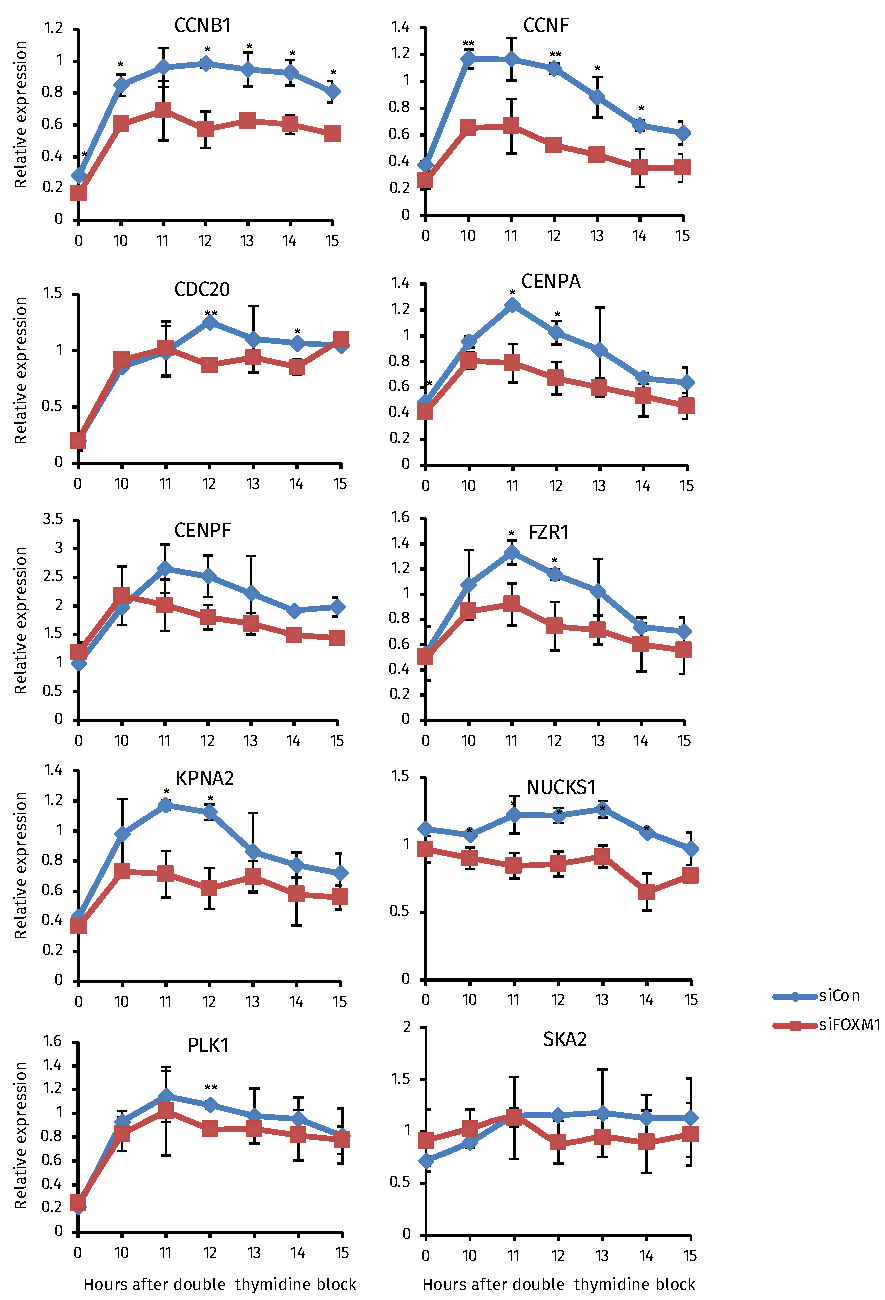
\includegraphics[width=0.9\textwidth]{chapter3/figures_foxm1/fig21.pdf}
    \caption[The expression pattern of FOXM1 target genes in the G2 and M phases of the cell cycle upon FOXM1 depletion]{\textbf{The expression pattern of FOXM1 target genes in the G2 and M phases of the cell cycle upon FOXM1 depletion.} U2OS cells were transfected with either a non-targeting siRNA or siRNA against FOXM1. Then cells were synchronised by double thymidine block and released into fresh media to allow the progression to G2 and M phase. Total RNA was collected at indicated time points after the release, and the mRNA levels were measured by RT-qPCR using gene-specific primers. The expression levels were first normalised by the 12h time point of the siCon sample, and then normalised by the expression of the reference gene \textit{HMBS}. The error bars represent standard deviations from two independent experiments. The P-value was calculated using a t-test. * and ** represent P<0.05 and P<0.01, respectively.}
    \label{fig:fig21}
\end{figure}

In summary, the FOXM1 ChIP-seq data suggests that it controls the expression of a large array of cell cycle regulated genes which are critical for mitosis and chromosome segregation. This is consistent with the previous notion of FOXM1 that it is one of the master regulators of G2-M cell cycle events (\cite{laoukili2005foxm1}). Our data has added a large number of novel target genes to the FOXM1 regulome.

\subsection{The CHR motif, not the canonical Forkhead motif, is enriched in the FOXM1 cistrome}

Having confirmed that FOXM1 controls the transcription of a large array of G2-M genes, the mechanism of the regulation was investigated. FOXM1 is a transcription factor, and transcription factors can make direct contacts with DNA. Therefore, it is logical to assume that FOXM1 regulates its target genes by directly binding to the DNA within the regulatory regions of its target genes.

To test this hypothesis, a \textit{de novo} motif discovery program, HOMER (\cite{heinz2010simple}), was used to find the overrepresented DNA sequences within 200 bp centred on the summits of FOXM1 ChIP-seq derived peaks. Since FOXM1 belongs to the Forkhead transcription factor family, we expected to find motifs similar to the Forkhead consensus RYMAAYA, as this was the case in the ChIP-seq studies of other Forkhead transcription factors like FOXO3 (\textbf{Figure \ref{fig:fig14}C}), FOXK2 (\cite{ji2012the}), FOXA1 (\cite{hurtado2011foxa1}), and FOXP3 (\cite{katoh2011foxp3}). However, the motif discovery failed to detect overrepresentation of canonical Forkhead consensus. Instead, two other motifs, the CCAAT-box motif and the CHR motif, were significantly enriched within the FOXM1 peaks (\textbf{Figure \ref{fig:fig22}A}).

The finding that the canonical Forkhead consensus RYMAAYA is not enriched within the FOXM1-bound regions is quite surprising. To confirm the reliability of this discovery, a traditional motif finding program MEME (\cite{bailey1994fitting}) was used to perform \textit{de novo} motif discovery from the ChIP-seq derived peaks of FOXM1. In agreement with HOMER, the top two motifs found by MEME were also the CCAAT-box motif and the CHR motif (\textbf{Figure \ref{fig:fig22}B}). In addition, a GC-rich motif was also returned by MEME, but not by HOMER. The reason that HOMER did not find the GC-rich motif was probably because HOMER, by default, randomly chooses background sequences whose GC-content is similar to the target sequences from the interrogated genome. Since most FOXM1 binding peaks are located within CpG islands (77\%), the background will be chosen from GC-rich regions from the genome as well. Therefore, the GC-rich motif might not be enriched in the FOXM1 binding regions compared to the background sequences. Indeed, when randomly chosen background sequences from the genome without the consideration of GC-content are used, HOMER also returned a GC-rich motif like MEME (data not shown).

\begin{figure}[!h]
    \centering
    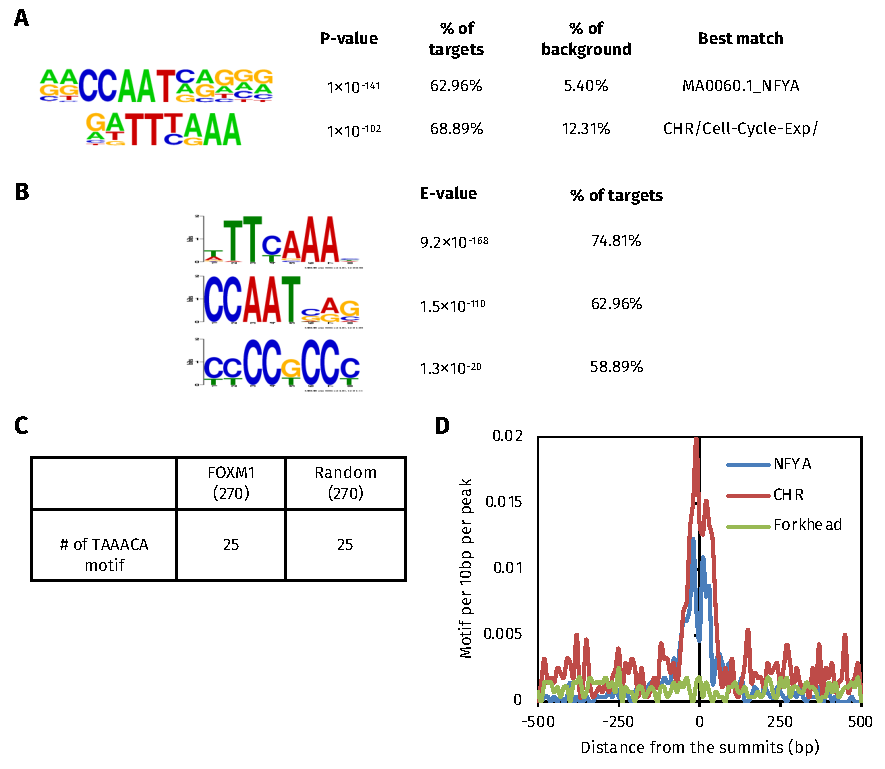
\includegraphics[width=0.9\textwidth]{chapter3/figures_foxm1/fig22.pdf}
    \caption[Motif discovery and analyses of FOXM1 peaks]{\textbf{Motif discovery and analyses of FOXM1 peaks. (A)} Two significantly enriched motifs returned by HOMER. The P-value was calculated based on the hypergeometric distribution. The percentage of target sequence and background sequence containing the indicated motif are also shown. Motif alignment against a custom collection of transcription factor motif database (\cite{heinz2010simple}) is shown in the \textbf{Best match} column. \textbf{(B)} Three significantly enriched motifs returned by MEME. The E-value and the percentage of target sites containing the motif are shown. The E-value returned by MEME is an estimate of the number of motifs one would expect to find by chance if the target sequences are shuffled. \textbf{(C)} Number of FOXM1 peaks or background sequence containing the sequence TAAACA. \textbf{(D)} The frequency of occurrence of the indicated motifs around the FOXM1 summits. FOXM1 ChIP-seq derived peaks were aligned by their summits, and a region of -500 bp and +500 bp relative to the summit was selected. Motif frequency was counted at every 10 bp bin. For the Forkhead site, the RYMAAAYA sequence was searched; for the NFYA motif and the CHR motif, the matrix shown in \textbf{(A)} was searched.}
    \label{fig:fig22}
\end{figure}

Since the hexamer sequence TAAACA was previously shown to be bound by FOXM1 \textit{in vitro} by selection and amplification of binding sites (\cite{korver1997the}), we searched the occurrence of the motif TAAACA with the 200 bp DNA sequences centred on the 270 FOXM1 summits. For parallel comparison, a random set of 270 sequences 200 bp in length and with a similar genomic distribution to the FOXM1 270 peaks were chosen from the genome as background sequences. The motif search showed that there were, indeed, only 25 FOXM1 peaks containing at least one TAAACA motif, but there were also 25 background sequences containing the motif (\textbf{Figure \ref{fig:fig22}C}). This clearly indicates that the presence of the TAAACA motif within the FOXM1 peaks is random, and there is no enrichment of this motif.

The summit (highest point where tags pile up) of the peak normally reflects the crosslinked point, hence the protein-DNA interaction site, and the most overrepresented DNA motif is generally believed to be the sequence bound by the protein. Therefore, in a typical ChIP- seq data, the enriched DNA motifs bound by the protein are regularly more frequent near the summit than the surrounding area (\cite{zhang2008model-based}). To further investigate whether the canonical Forkhead motif might be bound by FOXM1, the frequency of the motif occurrence around the FOXM1 summits was counted. Consistent with the motif search, the Forkhead motif is dispersed throughout the regions. In contrast, both the CCAAT-box motif and the CHR motif occurred much more frequently near the summit, although their frequency curves did not peak at the exact summit point (\textbf{Figure \ref{fig:fig22}D}). The CHR motif was even more frequent than the CCAAT-box motif at these locations.

\begin{figure}[!h]
    \centering
    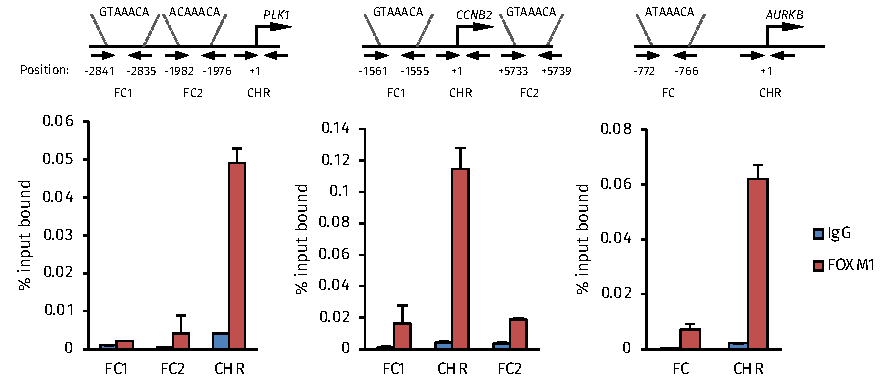
\includegraphics[width=0.9\textwidth]{chapter3/figures_foxm1/fig23.pdf}
    \caption[FOXM1 binding at different regions of the PLK1, CCNB2 and AURKB promoters]{\textbf{FOXM1 binding at different regions of the \textit{PLK1}, \textit{CCNB2} and \textit{AURKB} promoters.} ChIP-qPCR analysis of FOXM1 binding at different regions on the promoter of its target genes. ChIP was performed in U2OS cells using a FOXM1 antibody. A non- specific IgG antibody was also included as a control. Primers are indicated as arrows. The Forkhead consensus sequences (FC) and their positions are shown. Error bars of the \textit{PLK1} and \textit{CCNB2} loci represent the standard deviations from two independent experiments. Error bars of the \textit{AURKB} locus is the standard deviation from two technical replicates of qPCR in one experiment.}
    \label{fig:fig23}
\end{figure}

To experimentally validate that the Forkhead consensus is not enriched in FOXM1- bound peaks, three well-defined FOXM1 target genes, \textit{CCNB2, PLK1 and AURKB} were chosen, and primers were designed to target different regions of their promoters which contain both the Forkhead consensus and the CHR motif (\textbf{Figure \ref{fig:fig23}}). Then FOXM1 ChIP experiments were performed, and the binding at those regions was detected using qPCR. Consistent with previous results, the binding signals of FOXM1 were highest around the transcription start sites of those genes, where the CHR motif is located (\textbf{Figure \ref{fig:fig23}}). Although some binding was able to be detected at the regions where the Forkhead consensus located comparing to a non-specific IgG IP, the signals were at a low level (\textbf{Figure \ref{fig:fig23}}), possibly due to incomplete sonication of the DNA surrounding the binding locus. This reinforces the motif discovery results from an experimental point of view.

In summary, the canonical Forkhead consensus RYAAAYA motif is not enriched in the FOXM1 cistrome. Instead, the CCAAT-box, which has been shown bound by the transcription factor NF-Y, and the CHR motif are enriched in the FOXM1-bound regions. Moreover, the CCAAT-box and the CHR motif occur more frequently near the summits than the surrounding area, indicating FOXM1 is actually associated with these two motifs in vivo. Therefore, it seems that the data do not support our original assumption that FOXM1 regulates target genes by directly binding the DNA through motifs generally associated with the Forkhead protein binding in their regulatory elements.

\subsection{FOXM1 does not directly bind to the CHR motif}

Given that the CCAAT-box and the CHR motif are overrepresented within the FOXM1- bound regions, we next began to investigate whether FOXM1 can directly bind to either of these DNA motifs.

We first reasoned that the CCAAT-box has been shown bound by the transcription factor NF-Y (reviewed in \cite{mantovani1999the}), and this motif is prevalent in the promoters of many cell cycle genes, not specific for G2-M genes. It is unlikely that FOXM1 can directly bind to this DNA sequence (see below).

We then noticed that the CHR motif, to some extent, resembles the canonical Forkhead consensus: both of them are AT-rich DNA motifs. Previous studies suggest that FOXM1 binds to the canonical Forkhead consensus at an extremely low affinity (\cite{freddie2007functional,littler2010structure}). Therefore, it was possible that FOXM1 can somehow directly bind to the CHR motif to regulate the transcription of its target genes.

To check whether this is the case, band shift experiments were performed using a 6$\times$His and FLAG-tagged FOXM1 DNA-binding domain purified from bacteria. We first tested the interaction between the FOXM1 DNA-binding domain and the DNA sequence from the \textit{PLAC8} locus, which contains a canonical Forkhead consensus GTAAACA (\textbf{Figure \ref{fig:fig24}A}). FOXK2 and FOXO3 DNA-binding domains which were purified from bacteria in a similar way were used as positive controls (\textbf{Figure \ref{fig:fig24}B}). When added at 90 nM concentrations, clear FOXK2-DNA and FOXO3-DNA complexes were observed (\textbf{Figure \ref{fig:fig24}C}, lanes 2 and 3), but a FOXM1-DNA complex could not be detected (\textbf{Figure \ref{fig:fig24}C}, lane 4). With the concentration of FOXM1 DNA-binding domain increased to 900 nM, a weak protein-DNA complex was detected when the DNA sequences from the wild-type \textit{PLAC8} or \textit{MMP9} loci was used (\textbf{Figure \ref{fig:fig24}D}, lanes 2 and 5). After the addition of FLAG antibody, the intensity of protein-DNA complex significantly reduced, indicating that the complex was genuine FOXM1-DNA (\textbf{Figure \ref{fig:fig24}D}, lanes 3 and 6). However, a super-shift was not observed, presumably due to the unstable interactions of the FLAG antibody/FOXM1/DNA ternary complex. In addition, the FOXM1-DNA interaction was indeed a specific binding between FOXM1 and the canonical Forkhead consensus, because when the GTAAACA sequence in the wild-type \textit{MMP9} promoter was mutated to GTAAAAA, FOXM1 failed to form a complex with the mutated DNA sequence (\textbf{Figure \ref{fig:fig24}D}, lanes 8 and 9). More importantly, when a DNA sequence from the wild-type \textit{CCNB1} promoter, which contains the CHR motif, was added to the reactions, the FOXM1-DNA complex was undetectable (\textbf{Figure \ref{fig:fig24}D}, lanes 11 and 12).

The bandshift experiments suggest that FOXM1 cannot directly bind to the CHR motif. However, in this kind of experiment, only purified FOXM1 DNA-binding domain was tested. There are still possibilities that FOXM1 can make direct interaction with the CHR motif: (1) the full-length FOXM1 protein can bind to the CHR motif; (2) post-translational modifications might assist its binding to the CHR motif; (3) interactions with other proteins switch its binding specificity making FOXM1 directly bind to the CHR motif, a common mechanism utilised by many transcription factors to enhance specificity (\cite{siggers2011non-dna-binding,slattery2011cofactor}).

\begin{figure}[!h]
    \centering
    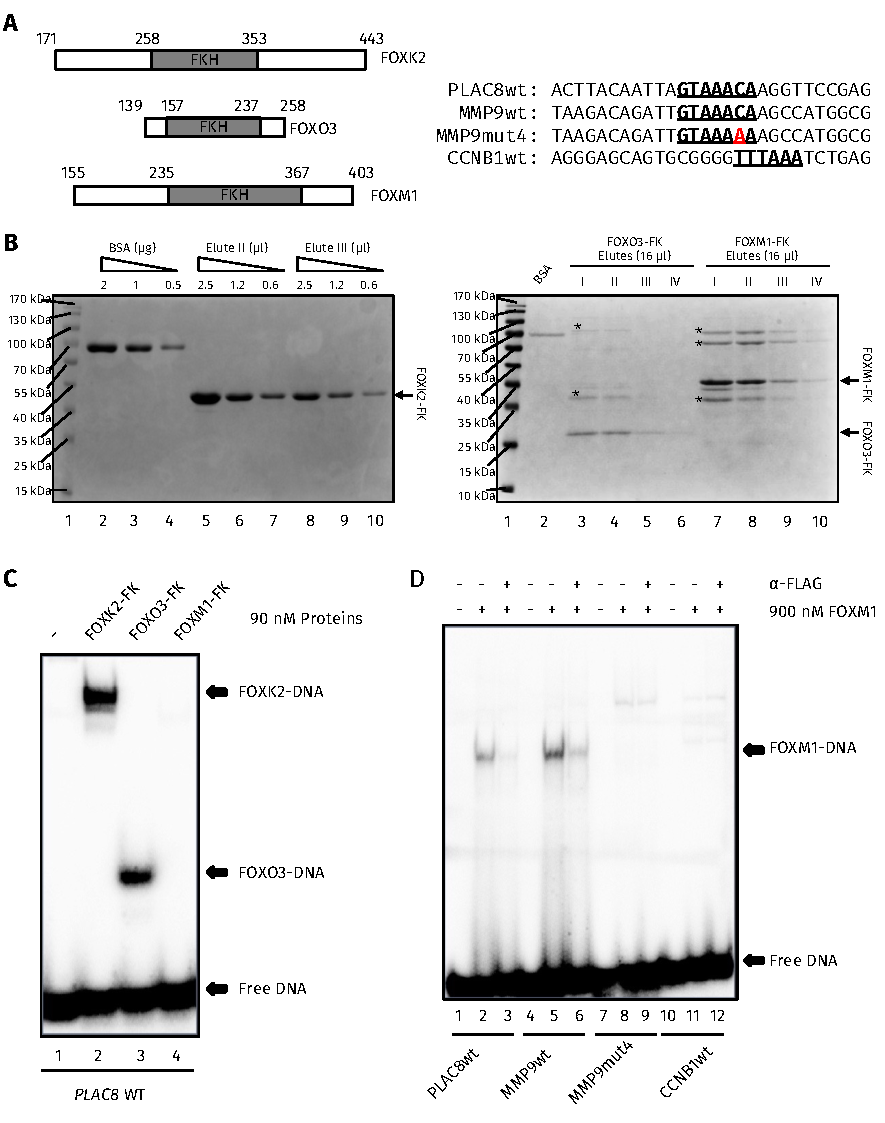
\includegraphics[width=0.9\textwidth]{chapter3/figures_foxm1/fig24.pdf}
    \caption[Bandshift experiments of \textit{in vitro} DNA-binding of Forkhead proteins]{\textbf{Bandshift experiments of \textit{in vitro} DNA-binding of Forkhead proteins. (A) Left,} schematic view of the Forkhead proteins used in the experiments. The numbers on the protein schematics delineate the amino acids at the start and the end of the fragments relative to the full-length protein. The position of the Forkhead DNA binding domain (FKH) is also indicated. \textbf{Right,} the DNA sequences from indicated loci used in the experiments. The motifs within the DNA sequences are underlined, and the mutation in the MMP9 locus-derived sequence is shown in red. \textbf{(B)} The Coomassie staining of the gels which contain purified DNA-binding domain of FOXK2 (left), FOXO3 and FOXM1 (right). Varying amounts of BSA and elutes of different proteins were run as indicated. The Molecular weight of the marker band is shown. Asterisks indicate possible non-specific proteins pulled down during the His tag purification. \textbf{(C)} The binding between the DNA sequence from \textit{PLAC8} locus and the DNA-binding domains of indicated Forkhead proteins. Proteins were added at 90 nM concentration. The binding reactions were run on a non-denaturing poly-acrylamide gel. The free DNA and the protein-DNA complexes are indicated by arrows. \textbf{(D)} The interaction between FOXM1 and DNA sequences from the indicated loci. The FOXM1 DNA- binding domain was added at 900 nM concentration. A FLAG antibody was added where indicated. The free DNA and the FOXM1-DNA complexes are indicated by arrows.}
    \label{fig:fig24}
\end{figure}

To investigate these possibilities, an \textit{in vitro} DNA pull-down assay was carried out. In this experiment, the wild-type DNA sequence from the \textit{CCNB1} promoter or various mutated versions were coupled with a biotin tag. The biotin-tagged DNA sequence was bound to streptavidin-linked magnetic beads, followed by the incubation with the cell extract from U2OS cells. After washing off the non-specific binding proteins, elutes were analysed using SDS-PAGE, and the bound proteins were detected by western blot using specific antibodies. A DNA sequence from a part of the luciferase gene was used as a negative control (\textbf{Figure \ref{fig:fig25}A}). The \textit{CCNB1} promoter sequence used in this experiment contains three well-defined motifs: the CCAAT-box motif which is bound by the transcription factor NF-Y, a CDE-like GC-rich motif which is important for the transcription of some, if not all, G2-M genes, and the CHR motif (\textbf{Figure \ref{fig:fig25}B}). Each of these was mutated individually and in a combined manner to assess the potential impact on FOXM1 binding.

\begin{figure}[!h]
    \centering
    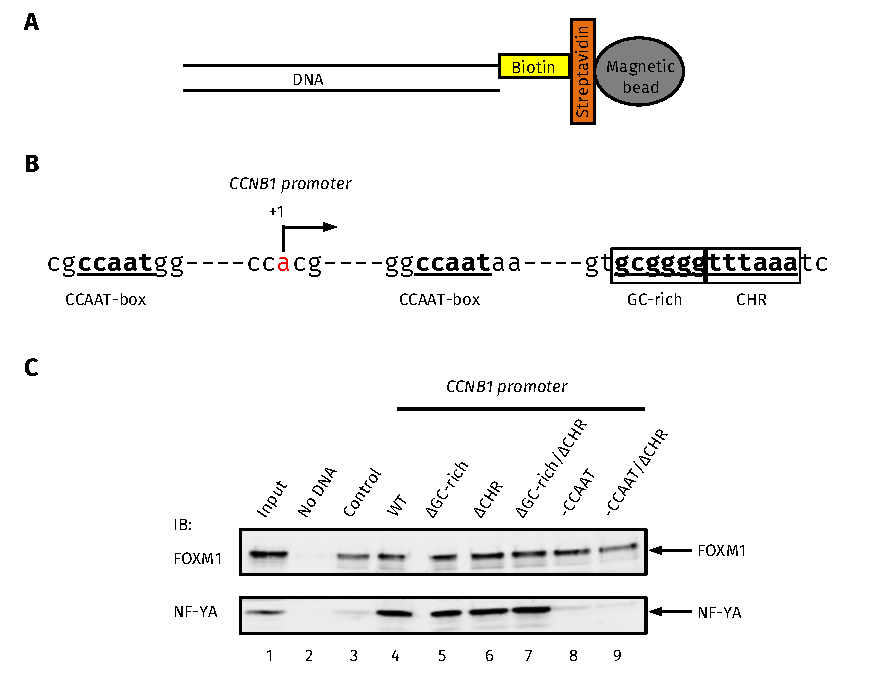
\includegraphics[width=0.9\textwidth]{chapter3/figures_foxm1/fig25.pdf}
    \caption[\textit{In vitro} DNA pull-down assay to investigate FOXM1-DNA interactions]{\textbf{\textit{In vitro} DNA pull-down assay to investigate FOXM1-DNA interactions. (A)} Schematic view of linking biotin-tagged DNA sequence to the streptavidin conjugated magnetic beads to generate the bait for the pull-down experiment. \textbf{(B)} The DNA sequence of \textit{CCNB1} promoter used in the pull-down experiments. The two CCAAT-boxes, the GC-rich, and the CHR motifs are shown, and the rest part of the promoter is omitted. The arrow indicates the transcription start site according to RefSeq. \textbf{(C)} DNA pull-down experiment to test the DNA-binding of FOXM1 and NF-YA. U2OS cell extracts were incubated with the indicated DNA sequences which were linked to the magnetic beads. The precipitated material was immunoblotted (IB) with the indicated antibodies. \enquote{$\Delta$} indicates the mutation of the motif, and \enquote{-} indicates the deletion of the motif. A fragment of DNA from the luciferase coding sequence was used as control.}
    \label{fig:fig25}
\end{figure}

As expected, the transcription factor NF-YA was able to bind the wild-type \textit{CCNB1} promoter sequence (\textbf{Figure \ref{fig:fig25}C}, lane 4). When the GC-rich or CHR motif was mutated, it still bound to the DNA sequence (\textbf{Figure \ref{fig:fig25}C}, lanes 5, 6 and 7), but lost its binding after the CCAAT-box motif was mutated (\textbf{Figure \ref{fig:fig25}C}, lanes 8 and 9). This is consistent with previous research showing that NF-YA bound to the CCAAT-box motif, and this binding was independent of the GC-rich and CHR motifs (\cite{müller2012the}). In contrast, the binding signals of FOXM1 remained relatively constant among the wild-type and all mutant promoter sequences (\textbf{Figure \ref{fig:fig25}C}, lanes 4 to 9), and the binding levels to the wild-type \textit{CCNB1} promoter sequence was very similar to the control DNA sequence (\textbf{Figure \ref{fig:fig25}C}, lane 3). In the absence of any DNA, no binding signal was detected (\textbf{Figure \ref{fig:fig25}C}, lane 2), indicating that the observed FOXM1 binding was due to the interaction with DNA, not the beads. Therefore, it seems that the affinity of FOXM1 binding to the \textit{CCNB1} promoter sequence is comparable to its non-specific DNA interaction. We are unable to observe sequence-specific binding of FOXM1 or any particular roles of the CHR motif in this binding.

In summary, FOXM1 can directly bind to the canonical Forkhead consensus \textit{in vitro}, even though the Forkhead consensus is not enriched in the ChIP-seq derived FOXM1 peaks. The affinity of FOXM1 for the Forkhead consensus is extremely low, but the interaction is still specific, because a single nucleotide mutation of the Forkhead consensus results in the loss of binding. However, in the in vitro experiments, we have found no evidence that FOXM1 binds to the DNA sequences it occupies \textit{in vivo}. It is therefore likely that a proper genomic context and/or the association with other factors are required for the FOXM1-DNA binding.

\subsection{The DREAM complex and the transcription factor NF-Y do not significantly contribute to FOXM1 DNA binding}

Since FOXM1 fails to make stable contacts with the CCAAT-box and the CHR motifs \textit{in vitro}, we next investigate how these two motifs recruit FOXM1 to the DNA in the cells, and how FOXM1 applies its regulatory roles via them.

The CCAAT-box motif is a NF-Y binding site. Although a previous study suggests that LIN54 can directly bind to the CHR motif \textit{in vitro}, due to technical difficulties of getting recombinant LIN54 protein \textit{in vitro}, the evidence is not convincing (\cite{schmit2009lin54}). On the other hand, a most recent study has demonstrated that the cell cycle regulatory complexes DREAM and MMB require an intact CHR to bind the promoter of many cell cycle genes (\cite{müller2012the}). Therefore, it is reasonable to speculate that either NF-Y or DREAM/MMB recruits FOXM1 to the DNA.

To test this hypothesis, GFP-tagged FOXM1B or FOXM1C isoform were transfected into HEK293 cells, and co-immunoprecipitation was performed using an anti-GFP antibody. The NF-Y is a trimeric transcription factor containing NF-YA, NF-YB, and NF-YC, with NF-YA being the direct DNA-binding subunit, and all three subunits are required for the binding to CCAAT-box (\cite{sinha1996three}). Here, we used NF-YA as a representation of the NF-Y transcription factor. LIN9 and LIN37 were used to represent the MuvB core complex. Clear interactions between both FOXM1 isoforms and LIN9/LIN37 were observed (\textbf{Figure \ref{fig:fig26}A}). The MMB-specific subunit B-MYB was also co-immunoprecipitated with the two FOXM1 isoforms (\textbf{Figure \ref{fig:fig26}A}). However, we were unable to detect interactions of FOXM1 with either of the DREAM-specific subunits E2F4 and p130 (\textbf{Figure \ref{fig:fig26}A}), indicating that FOXM1 does not form stable complex with the DREAM proteins. This is in agreement with the previous findings that the DREAM complex is only present in quiescent cells, while FOXM1 is only expressed in proliferating cells (\cite{litovchick2007evolutionarily,korver1997the}). Similarly, no detectable interactions between the two FOXM1 isoforms and NF-YA could be observed (\textbf{Figure \ref{fig:fig26}A}).

The co-immunoprecipitation indicated that the DREAM complex and the transcription factor NF-Y might not contribute to the DNA-binding of FOXM1. To further confirm these findings, FOXM1 binding to several promoter regions was measured by ChIP-qPCR in U2OS cells after the transfection with a non-targeting siRNA or siRNAs against either E2F4 or NF-YA. Consistent with the negative Co-IP data, knockdown of E2F4 or NF-YA did not significantly change the binding of FOXM1 (\textbf{Figure \ref{fig:fig26}B}).

\begin{figure}[!h]
    \centering
    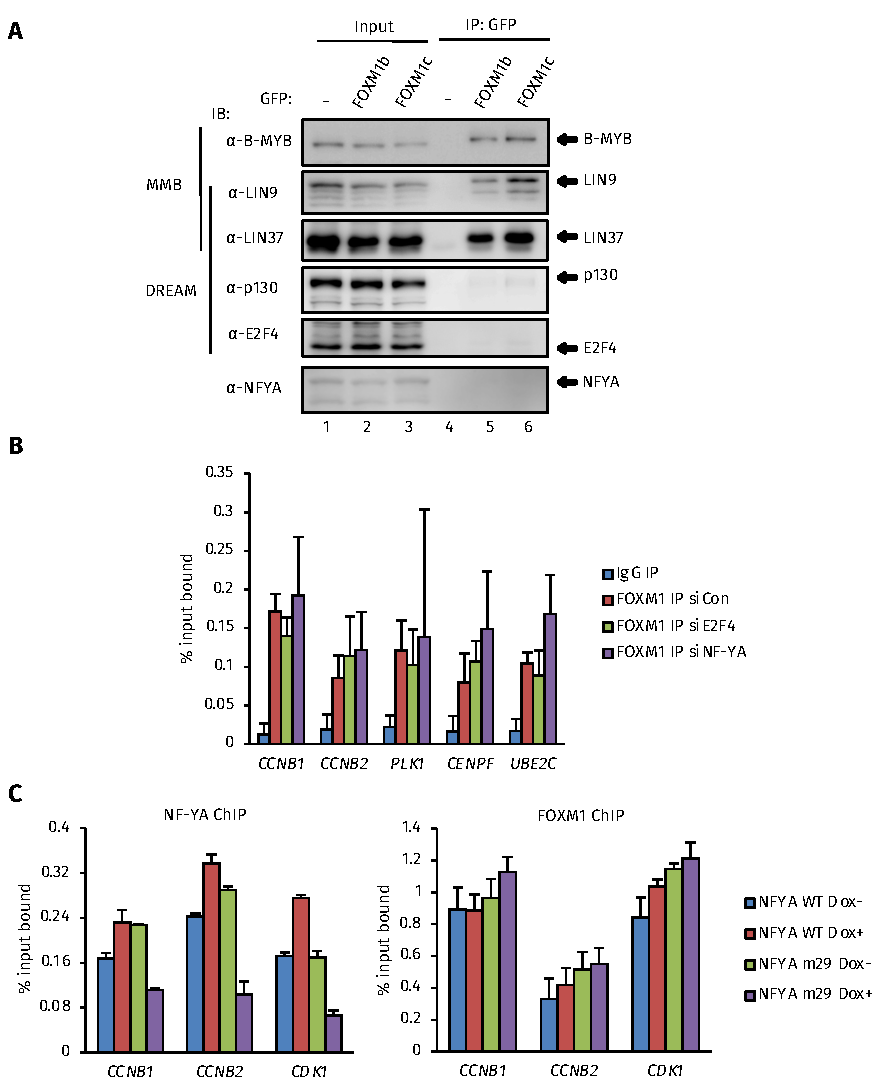
\includegraphics[width=0.9\textwidth]{chapter3/figures_foxm1/fig26.pdf}
    \caption[FOXM1 interacts with the MMB complex, but not the DREAM complex or NF-Y]{\textbf{FOXM1 interacts with the MMB complex, but not the DREAM complex or NF-Y. (A)} Co-immunoprecipitation of two FOXM1 isoforms with the DREAM/MMB complexes and NF-YA. Plasmids encoding GFP tagged FOXM1B or FOXM1C were transfected into HEK293 cells, and the protein complexes were precipitated with an anti-GFP antibody. The immunoprecipitations were blotted (IB) with indicated antibodies. These experiments were done by Dr. Gerd Muller. \textbf{(B)} ChIP experiments of FOXM1 after the knockdown of E2F4 or NF-YA. U2OS cells were transfected with 20 nM of the indicated siRNAs. 48 hours after the transfection, ChIP experiments were performed using a FOXM1 or non-specific IgG antibody. Error bars represent the standard deviations from two independent experiments. \textbf{(C)} FOXM1 and NF-YA ChIP experiments after the overexpression of either wild-type NF-YA (NFYA WT) or a dominant negative form of NF-YA (NFYA m29). The HEK293 stable cell lines were treated where indicated with 1 $\mu$g/mL doxycycline for 24 hours. ChIP experiments were performed using NF-YA (left) or FOXM1 (right) antibodies. Error bars represent the standard deviation from two independent experiments.}
    \label{fig:fig26}
\end{figure}

In addition, we also investigated the relationship between of NF-Y and FOXM1 DNA binding by using HEK293 stable cell lines which expresses either wild-type NF-YA or a dominant-negative NF-YA (NF-YA m29) under the control of a tetracycline-inducible CMV promoter (\cite{tiwari2011a}). The dominant-negative form of NF-YA is unable to bind DNA, and will interfere with the endogenous NF-YA DNA binding when overexpressed (\cite{mantovani1994dominant}). FOXM1 ChIP experiments were performed and its DNA binding was measured by qPCR with or without the overexpression of the wild-type NF-YA or the dominant negative form of NF-YA. The overexpression of the dominant negative form of NF-YA indeed resulted in a reduced overall binding of NF-YA when a NF-YA antibody was used in the ChIP experiments (\textbf{Figure \ref{fig:fig26}C}, left). However, no accompanying decrease of FOXM1 binding was observed (\textbf{Figure \ref{fig:fig26}C}, right), which is in agreement with the siRNA experiments mentioned before. Similarly, wild-type NF-YA overexpression resulted in an slightly increase in NF-YA binding to the tested promoter regions but had little effect on FOXM1 binding (\textbf{Figure \ref{fig:fig26}C}).

In summary, we were unable to detect stable interactions between FOXM1 and either the DREAM complex or NF-YA. More importantly, knockdown of the DREAM components and NF-YA or overexpression of a dominant-negative form of NF-YA hardly changed the ChIP signals of FOXM1, indicating that they do not contribute greatly to FOXM1 chromatin binding \textit{in vivo}. Hence the over-representation of the CCAAT-box motif is probably due to its common co-occurrence with the CHR motif in the promoter of G2-M genes (\cite{müller2012the}). The interactions of FOXM1 with the MuvB core proteins and the MMB-specific protein B-MYB were clearly detected, indicating the MMB complex is likely to play important role on FOXM1 DNA binding.

\subsection{The CHR motif recruits FOXM1 to chromatin and is important for FOXM1-mediated transcriptional activation}

Having confirmed that the DREAM complex and NF-YA hardly contribute to FOXM1 chromatin binding, we focused on investigating the potential roles of the CHR motif and the MMB complex on the chromatin binding of FOXM1. To this end, we first started with establishing the importance of the CHR motif in recruiting FOXM1 to its regulatory regions.

Within the 270 FOXM1 peaks, there were 173 peaks (CHR+) which contain the CHR motif. When compared to the rest 97 peaks (CHR-) which do not contain the CHR motif, the average binding signals at the CHR+ peaks were generally higher than those at the CHR- peaks (\textbf{Figure \ref{fig:fig27}A}), indicating that FOXM1 has higher occupancy at regions with CHR motif. Therefore, the mechanisms of the recruitment of FOXM1 to these two categories of peaks might be different.

\begin{figure}[!h]
    \centering
    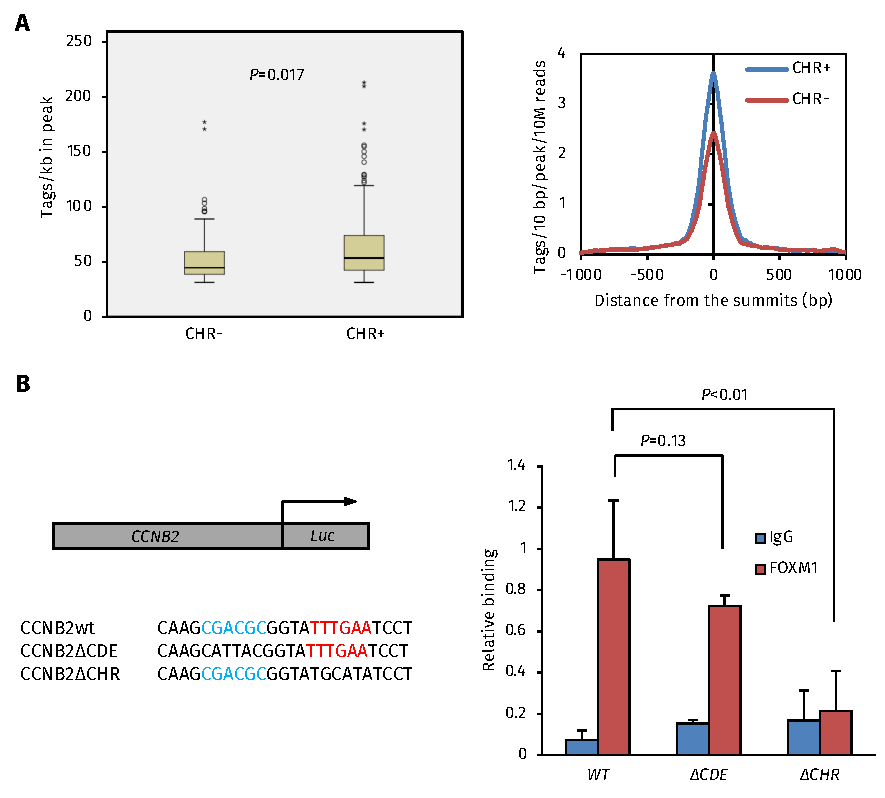
\includegraphics[width=0.9\textwidth]{chapter3/figures_foxm1/fig27.pdf}
    \caption[The CHR motif plays an important role in recruiting FOXM1 to chromatin]{\textbf{The CHR motif plays an important role in recruiting FOXM1 to chromatin. (A) Left,} boxplot of tags in peaks that contain the CHR motif (CHR+) and peaks that do not contain the CHR motif (CHR-). Peak length was normalised to 1 kb. P- value was calculated by an independent t-test. \textbf{Right,} quantification of average tags around the summits of peaks which have or do not have the CHR motif. Peaks were aligned by their summits, and a region of -1 and +1 kb relative to the summit was selected. Tags were calculated in every 10 bp bin across this region and normalised to tags per 10 million total reads per bin per peak. \textbf{(B) Left,} schematic view of the luciferase construct driven by the wild-type and mutated human \textit{CCNB2} promoters integrated in the HCT116 stable cell line. DNA sequences are shown below, and the motifs (CDE and CHR) are shown in colour. \textbf{Right,} ChIP-qPCR analyses of FOXM1 binding at the transgene regions in the HCT116 stable cell lines. The binding at the transgene regions were normalised to the binding signals at the endogenous \textit{CCNB2} locus (taken as 1). Error bars present the standard deviations from three independent experiments, and the P- values are indicated. These experiments were done by Ms. Marianne Quaas.}
    \label{fig:fig27}
\end{figure}

To check whether an intact CHR motif is required for the FOXM1 chromatin binding, HCT116 stable cell lines were previously generated which have luciferase constructs driven by the wild-type or mutant human \textit{CCNB2} promoters integrated into the genome (\textbf{Figure \ref{fig:fig27}B}, left; \cite{müller2012the}). A triple FLAG tagged FOXM1 was transfected into the stable cell lines, and the binding of FOXM1 to the regions of these transgenes was measured by ChIP-qPCR. FOXM1 was able to bind to the region of the wild-type \textit{CCNB2} promoter driven transgene. However, mutation of the CHR motif abolished the binding of FOXM1. In contrast, mutation of the CDE motif did not significantly affect FOXM1 binding ($p=0.13$) (\textbf{Figure \ref{fig:fig27}B}, right). This indicates that the recruitment of FOXM1 to chromatin is dependent on the CHR motif.

Given that the CHR motif is critical for the FOXM1 chromatin binding, we next checked whether it is also important for the FOXM1-mediated gene activation. Luciferase constructs driven by the wild-type or mutant human \textit{CCNB1} promoter and the \textit{FOXM1} expression plasmid were co-transfected into U2OS cells, and the luciferase activities were measured to assess the gene activation by FOXM1. Overexpression of \textit{FOXM1} resulted in more than 2-fold activation of the wild-type \textit{CCNB1} promoter-driven luciferase reporter. A similar level of activation was also observed when the CDE-like GC-rich motif was mutated (\textbf{Figure \ref{fig:fig28}A}). However, the activation was severely curtailed when the CHR motif was mutated, indicating that the CHR motif is critical for FOXM1-mediated transcriptional activation (\textbf{Figure \ref{fig:fig28}A}). Interestingly, when the CCAAT-box motif was deleted, FOXM1 was unable to activate the promoter (\textbf{Figure \ref{fig:fig28}A}). This is consistent with the previous notion that the CHR-containing G2-M genes require the transcription factor NF-Y for their activation (reviewed in \cite{müller2010the}). Therefore, it is likely that in the absence of NF-Y, the promoter will be completely shut down. Indeed, deletions of the CCAAT-box motifs led to \textasciitilde 50\% reduction of the basal promoter activity in cycling cells (\textbf{Figure \ref{fig:fig28}B}).

\begin{figure}[!h]
    \centering
    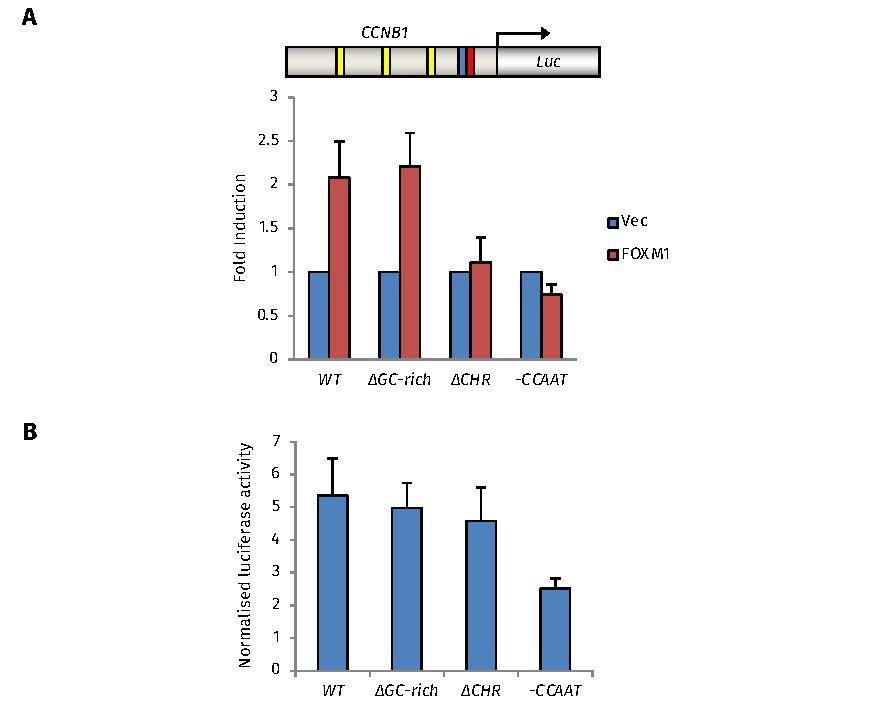
\includegraphics[width=0.9\textwidth]{chapter3/figures_foxm1/fig28.pdf}
    \caption[The CHR motif is important for the FOXM1-mediated transcriptional activation]{\textbf{The CHR motif is important for the FOXM1-mediated transcriptional activation. (A) Top,} schematic view of the luciferase construct driven by the human \textit{CCNB1} promoter. The CHR motif (red), the GC-rich motif (blue) and the CCAAT-box motif (yellow) are indicated. \textbf{Bottom}, luciferase assays in U2OS cells after the overexpression of FOXM1. The activities of luciferase driven by the indicated \textit{CCNB1} promoters were normalised by the protein concentrations of the extracts. The activity of the indicated luciferase construct was shown relative to the activity of each construct in the presence of the control vector (taken as 1). Error bars represent the standard deviation from two independent experiments. \textbf{(B)} The basal luciferase activity of the indicated construct. The luciferase activities without the overexpression of FOXM1 were normalised to the activities of $\beta$-Gal constructs. Error bars represent the standard deviation from two independent experiments.}
    \label{fig:fig28}
\end{figure}

In summary, FOXM1 has generally higher occupancy at the regions containing the CHR motif. Though not directly bound by FOXM1 \textit{in vitro}, an intact CHR motif is required for not only the DNA recruitment of FOXM1 \textit{in vivo}, but the transcriptional activation mediated by FOXM1 as well.

\subsection{The MMB complex assists the recruitment of FOXM1 to chromatin \textit{in vivo}}

Some evidence indicates that the MuvB core component LIN54 can directly bind to the CHR motif (\cite{schmit2009lin54}), and recent ChIP-seq analyses of the MMB components (LIN9 and B-MYB) have shown that the CHR motif is also enriched in the MMB bound regions (\cite{sadasivam2012the}). Moreover, an earlier study demonstrated that the binding of the MMB components to several G2/M gene promoters is dependent on an intact CHR motif (\cite{müller2012the}). Since physical interactions between FOXM1 and the MMB complex can be observed \textit{in vivo}, it is likely that FOXM1 and the MMB complex bind to the same promoters, and FOXM1 is indirectly recruited to the CHR motif by the MMB complex.

To test this hypothesis, we first compared the FOXM1 binding profile with the LIN9 and B-MYB ChIP-seq data performed in proliferating HeLa cells (\cite{sadasivam2012the}). In agreement with the previous results that FOXM1 interacts with the MMB complex, a large proportion of FOXM1 binding events (> 60\%) shared similar binding profiles with both LIN9 and B-MYB, though many FOXM1-specific peaks which did not overlap with LIN9 or B-MYB binding regions were also observed (\textbf{Figure \ref{fig:fig29}A}). Of note, such a great extent of overlap could still be an underestimation due to the different cell types used in these experiments (FOXM1 in U2OS cells, LIN9/B-MYB in HeLa cells). In addition, the LIN9 and B-MYB tags were nicely clustered around the summit of FOXM1 peaks (\textbf{Figure \ref{fig:fig29}A}, right), indicating these three factors bound to the same or very close positions. In addition, the CHR motif was more enriched in the FOXM1 peaks that are also bound by LIN9 and B-MYB compared to the FOXM1-specific peaks lacking evidence for the binding of these additional factors (\textbf{Figure \ref{fig:fig29}B}), further emphasising the links between the MMB-mediated regulation and the CHR motif. Interestingly, the average signal intensity around the FOXM1-specific peaks was generally lower than that of those which were shared with LIN9 and B-MYB (\textbf{Figure \ref{fig:fig29}A}, right). This implies that FOXM1 tends to have higher occupancy when it co-binds with LIN9 and B-MYB.

\begin{figure}[!h]
    \centering
    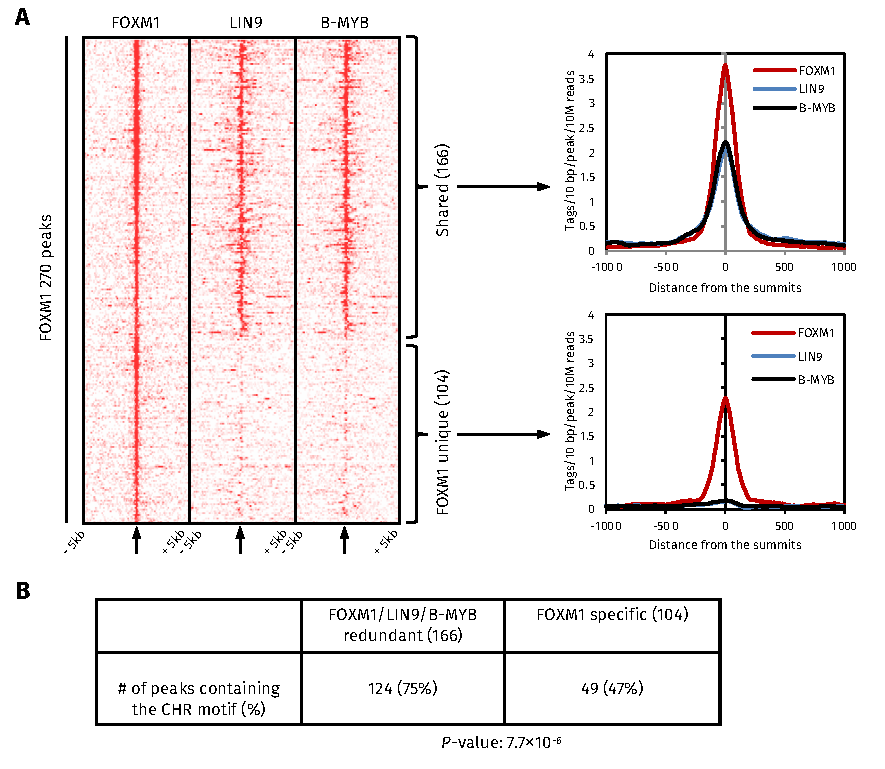
\includegraphics[width=0.9\textwidth]{chapter3/figures_foxm1/fig29.pdf}
    \caption[FOXM1 has both shared and specific binding events comparing to LIN9 and B-MYB binding]{\textbf{FOXM1 has both shared and specific binding events comparing to LIN9 and B-MYB binding. (A) Left,} heatmap of tag density profiles of FOXM1, LIN9 and B-MYB ChIP- seq experiments around the 270 FOXM1 peaks. Tags were calculated in every 50 bp bin, and the density profiles were normalised to tags per 10 million total reads per bin. The middle point of each panel (indicated by small arrows below) represents the summit of the peak. 5 kb upstream and 5 kb downstream around the summit of each FOXM1 peak were plotted. \textbf{Right,} quantification of average of tags around the summits of shared peaks and FOXM1 unique peaks. Peaks were aligned by the summits of FOXM1 peaks, and a region of -1 and +1 kb relative to the summit was selected. Tags were calculated in every 10 bp bin and normalised to tags per 10 million total reads per bin per peak. \textbf{(B)} Occurrence of the CHR motif in the FOXM1/LIN9/B-MYB shared peaks and the FOXM1-specific peaks. \textit{P}-value was calculated by Fisher's exact test and is shown below the table.}
    \label{fig:fig29}
\end{figure}

Having confirmed that most FOXM1 binding events are shared with LIN9 and B-MYB, we next investigated whether depletion of LIN9 or B-MYB would affect the DNA binding of FOXM1 \textit{in vivo}. To this end, siRNA against either LIN9 or B-MYB was transfected into U2OS cells, and FOXM1 ChIP experiments were performed after the transfection. The knockdown of LIN9 resulted in reduced binding of FOXM at several target genes, but the depletion of B-MYB hardly had any effects on FOXM1 binding (\textbf{Figure \ref{fig:fig30}A}, left). We did observe a certain degree of change of FOXM1 binding after B-MYB knockdown in individual experiments, but the change was not consistent between experiments. Hence it did not reach a statistically significant level (\textbf{Figure \ref{fig:fig30}A}, left). A recent study has shown that both LIN9 and B-MYB depletion will lead to reduced binding of FOXM1 (\cite{sadasivam2012the}). This partially agrees with our results, and the discrepancy in the effects of B-MYB knockdown on FOXM1 binding might be due to quite variable IP efficiencies in our experiments. However, the protein level of FOXM1 was slightly reduced after the depletion of LIN9 (\textbf{Figure \ref{fig:fig30}A}, right).

\begin{figure}[!h]
    \centering
    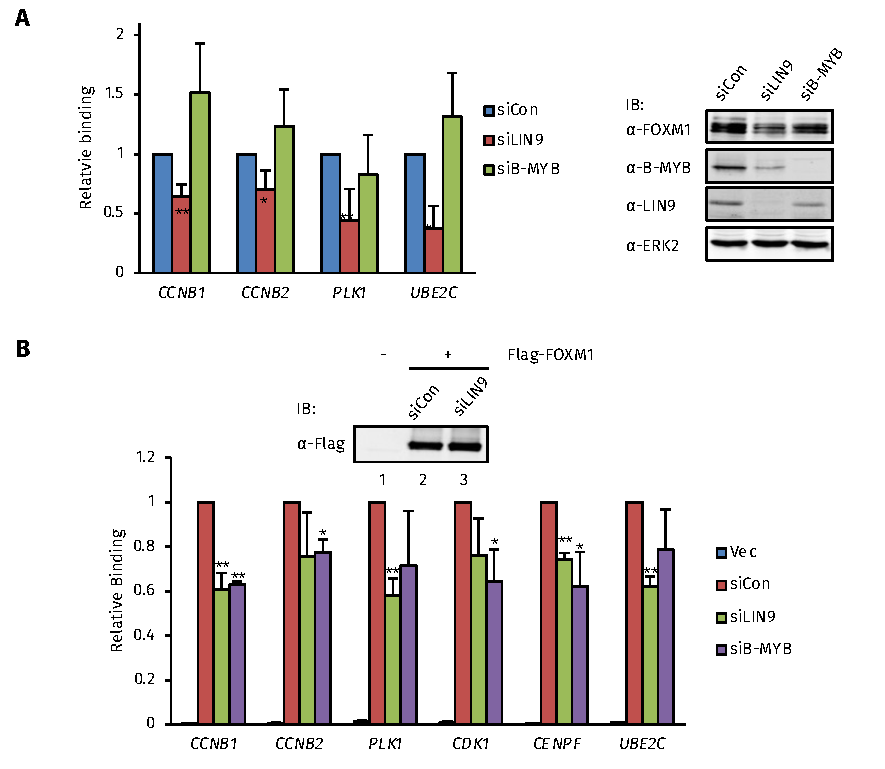
\includegraphics[width=0.9\textwidth]{chapter3/figures_foxm1/fig30.pdf}
    \caption[The binding of FOXM1 to promoter regions reduces after depletion of LIN9 or B-MYB]{\textbf{The binding of FOXM1 to promoter regions reduces after depletion of LIN9 or B-MYB. (A) Left,} endogenous FOXM1 binding at four target genes. ChIP experiments were performed in U2OS cells using a FOXM1 antibody after 48 hours transfection of the indicated siRNAs. Error bars represents the standard deviations of two independent experiments. P-value was calculated by t-test (* and ** represent $P<0.05$ and $P<0.005$, respectively). \textbf{Right,} western blot analysis showing the endogenous FOXM1 protein level after the depletion of LIN9 or B-MYB. U2OS cells were transfected with non-targeting control or FOXM1 siRNAs, protein expression levels were examined by western blot using the indicated antibodies. \textbf{(B)} FLAG-tagged FOXM1 binding at six target genes. ChIP experiments were performed in HEK293T cells transfected with FLAG-tagged FOXM1 (red, green and purple bars) or an empty vector (blue bars) using a FLAG antibody after the transfection of the indicated siRNAs. Error bars represents the standard deviations of two independent experiments. P-value was calculated by t-test (* and ** represent $P<0.05$ and $P<0.01$, respectively). The expression level of FLAG-tagged FOXM1 examined by western blot using a FLAG antibody was shown on the top.}
    \label{fig:fig30}
\end{figure}

To make sure the reduced FOXM1 binding after the depletion of LIN9 is not due to a change at the protein level, a triple FLAG-tagged FOXM1 was transfected into HEK293T cells after the knockdown of either LIN9 or B-MYB. Then FOXM1 ChIP experiments were performed using a FLAG antibody, and the binding of FOXM1 was measured by qPCR. The knockdown of LIN9 did not affect the level of overexpressed FOXM1 protein (\textbf{Figure \ref{fig:fig30}B}). Depletion of either LIN9 or B-MYB resulted in reduced binding signals of FOXM1 at a panel of its target genes, although some changes did not reach statistically significance (\textbf{Figure \ref{fig:fig30}B}). This indicates that the curtailed binding of FOXM1 is due to the loss of LIN9 and B-MYB, not the reduced protein level of FOXM1.

In summary, most FOXM1 binding events are shared with LIN9 and B-MYB, and the depletion of LIN9 or B-MYB leads to the reduced promoter binding of FOXM1, indicating the MMB complex is important for the recruitment of FOXM1 to promoters of its target genes.

\subsection{The MMB interaction domain within FOXM1 is important for its chromatin recruitment}

The loss of LIN9 or B-MYB protein leading to reduced binding of FOXM1 suggests that the protein-protein interactions between FOXM1 and the MMB complex are important for the recruitment of FOXM1 to the DNA. Therefore, we next mapped the MMB interaction region(s) in FOXM1 using GST pull down assays. To this end, GST-tagged truncated FOXM1B proteins were purified, and GST pull down assays were performed using U2OS total cell lysates with equal amount of different FOXM1 truncations (\textbf{Figure \ref{fig:fig31}A}).

The amount of different truncated proteins used per pulldown experiment was relatively equal, except FOXM1 aa 451-748 which has a lot of degradation (\textbf{Figure \ref{fig:fig31}A}, lane 9). The N-terminal parts of FOXM1 (aa 1-130 and 1-235) were not able to interact with LIN9/B-MYB (\textbf{Figure \ref{fig:fig31}A}, lanes 3 and 4). When the DNA-binding domain was included (aa 1-367), clear interactions with both LIN9 and B-MYB were observed (\textbf{Figure \ref{fig:fig31}A}, lane 5), indicating the FOXM1 DNA-binding domain (aa 235-367) is important for the LIN9/B-MYB interaction. However, when amino acids 1-116 were removed, the binding to LIN9/B-MYB was lost (\textbf{Figure \ref{fig:fig31}A}, lane 6), suggesting that the N-terminal domain (aa 1-116) is also critical for the LIN9/B-MYB binding. None of the rest of the FOXM1 truncations including the DNA-binding domain alone (aa 235-367) were able to interact with LIN9/B-MYB. These pulldown experiments indicate that FOXM1 aa 1-367 is sufficient for the MMB binding, and both the N-terminal (aa 1-116) and the DNA-binding domains (aa 235-367) are required for the interactions.

\begin{figure}[!t]
    \centering
    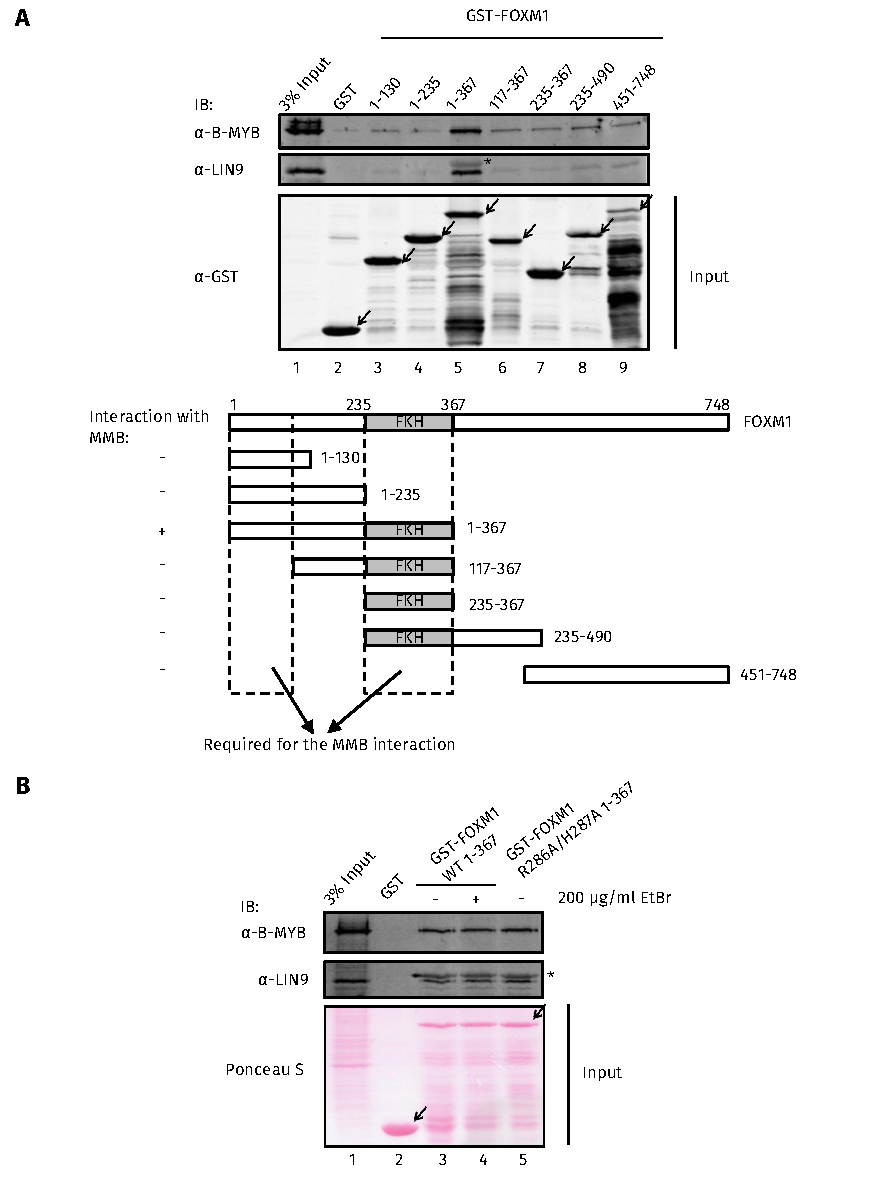
\includegraphics[width=0.9\textwidth]{chapter3/figures_foxm1/fig31.pdf}
    \caption[GST pull down experiments to map the MMB interaction regions in FOXM1]{\textbf{GST pull down experiments to map the MMB interaction regions in FOXM1. (A) Top,} GST pull down assays using different truncations of FOXM1 fused to GST with U2OS cell lysate. GST-tagged FOXM1 truncations were purified, and \textasciitilde 1 $\mu$g of each truncation was used per pulldown. After washing, the pulldowns were immunoblotted (IB) with the indicated antibodies. The $\alpha$-GST blot showed the amount of GST and GST-tagged FOXM1 truncations (black arrows) used in the pulldown assays. Asterisk indicates the cross-reaction of the LIN9 antibody with the GST fusion protein band. \textbf{Bottom,} schematic view of the FOXM1 constructs and MMB interaction regions in FOXM1. \textbf{(B)} GST pulldown assays using the indicated GST-FOXM1 fusion proteins with or without ethidium bromide (EtBr). Ponceau S staining showed relatively equal loading of GST and GST-tagged FOXM1 truncations (black arrows) used in the pulldown assays. Asterisk indicates the location of a cross-reacting band with the LIN9 antibody arising from the GST fusion protein.}
    \label{fig:fig31}
\end{figure}

To rule out the possibility that the interaction between FOXM1 and LIN9/B-MYB is mediated by DNA, the pulldown assay was repeated using GST-FOXM1 aa 1-367 in the presence of ethidium bromide. In addition, a DNA-binding domain mutant FOXM1 (R286A/H287A), which has been predicted to be unable to specifically bind to DNA according to the structure (\cite{littler2010structure}), was also included in the experiment as a control. The wild-type FOXM1 aa 1-367 could interact with LIN9 and B-MYB with or without ethidium bromide, and the DNA-binding domain mutant FOXM1 was still able to bind to LIN9 and B-MYB (\textbf{Figure \ref{fig:fig31}B}). These results indicate that FOXM1 is able to interact with the MMB complex \textit{in vitro}, and the interaction is indeed through protein- protein interactions and is not mediated by co-precipitating DNA.

To further substantiate our hypothesis that protein-protein interactions of FOXM1 with the MMB complex are critical for its DNA binding, we generated a construct of a triple FLAG tagged FOXM1 truncation (FOXM1 $\Delta$1-116), where the DNA binding domain of FOXM1 was kept intact, but the N-terminal amino acids 1-116 which are important for the MMB complex interaction were deleted (\textbf{Figure \ref{fig:fig32}A}). We argue that binding of FOXM1 ($\Delta$1-116) should not be as strong as the full-length FOXM1 protein if protein-protein interactions play an important role in its chromatin binding.

To investigate whether this is the case, we first checked the subcellular localisation of the truncated FOXM1 to ensure that it was still targeted to the nucleus. Immunofluorescence experiments were performed in U2OS cells after transfection of the triple FLAG-tagged FOXM1 proteins. The FOXM1 ($\Delta$1-116) protein was mainly located in the nucleus, as was also observed for the full-length protein (\textbf{Figure \ref{fig:fig32}A}), although some cytoplasmic staining was visible in both cases. This is in agreement with the previous finding that the nuclear localisation signal of FOXM1 is located at the C-terminal of its Forkhead DNA-binding domain (\cite{zhang2011foxm1}).

\begin{figure}[!h]
    \centering
    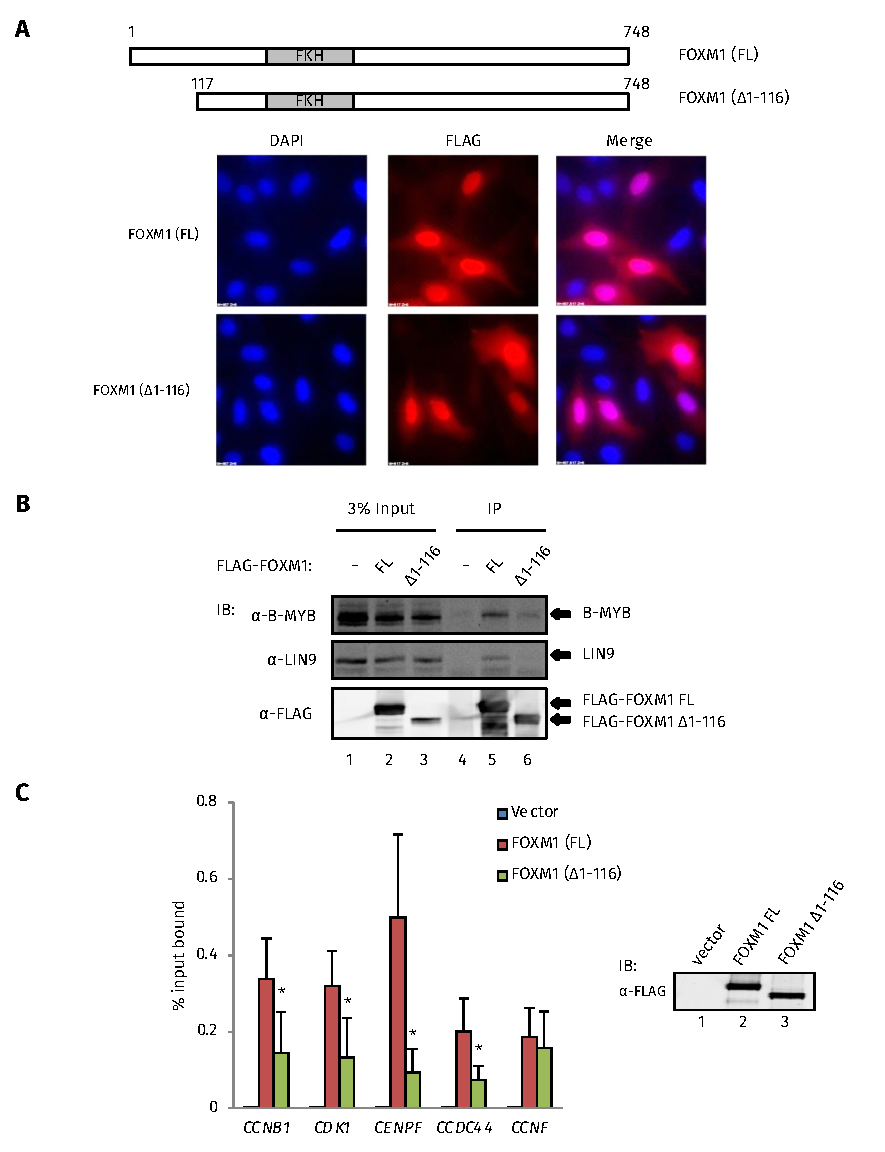
\includegraphics[width=0.9\textwidth]{chapter3/figures_foxm1/fig32.pdf}
    \caption[The MMB interaction regions in FOXM1 are important for the chromatin recruitment of FOXM1]{\textbf{The MMB interaction regions in FOXM1 are important for the chromatin recruitment of FOXM1. (A)} Immunofluorescence analyses showing the localisation of the full-length FOXM1 (FL) and FOXM1 ($\Delta$1-116) proteins. U2OS cells were transfected with the indicated constructs. Cells were incubated with FLAG antibody, and the signals were visualised by the Alexa Fluor 594-conjucated anti-mouse secondary antibody (red). DNA was stained with DAPI (blue). \textbf{(B)} Co-immunoprecipitation of the FOXM1 (FL) and FOXM1 ($\Delta$1-116) proteins with B-MYB and LIN9. The indicated FOXM1 protein constructs were transfected into U2OS cells, and associated complexes were co-precipitated with FLAG agarose. The immunoprecipitations were blotted (IB) with the indicated antibodies. \textbf{(C)} ChIP analyses of the binding of FOXM1 (FL) and FOXM1 ($\Delta$1-116) at the indicated loci. HEK293T cells were transfected with plasmids encoding the indicated proteins, and ChIP experiments were performed using an anti-FLAG antibody. Expression levels of the two proteins were tested by western blot with an anti-FLAG antibody. Error bars represent the standard deviation from three independent experiments. P-value was calculated using a t-test. * represents $P<0.05$.}
    \label{fig:fig32}
\end{figure}

Next, we tested the ability of the FOXM1 ($\Delta$1-116) protein to interact with the MMB complex by co-immunoprecipitation. Triple FLAG-tagged FOXM1 proteins were transfected into U2OS cells, and co-associated protein complexes were immunoprecipitated by FLAG agarose. Consistent with the GST pulldown assays, the interaction between B-MYB and FOXM1 ($\Delta$1-116) was severely curtailed compared to the full-length FOXM1 (\textbf{Figure \ref{fig:fig32}B}, top panel, lanes 5 and 6). The effect of the truncation on the interaction with LIN9 was even more prominent as no detectable LIN9 binding was observed with the FOXM1 ($\Delta$1-116) protein (\textbf{Figure \ref{fig:fig32}B}, middle panel, lane 6). Then to test the \textit{in vivo} chromatin binding ability of this truncated FOXM1 protein, the constructs were transfected into HEK293T cells, and ChIP experiments were performed using an anti-FLAG antibody. The expression level of the FOXM1 ($\Delta$1-116) was similar to the full-length protein (\textbf{Figure \ref{fig:fig32}C}, right panel). Consistent with the IP results, the binding of FOXM1 ($\Delta$1-116) was reduced at several tested regions compared to the full-length FOXM1 protein (\textbf{Figure \ref{fig:fig32}C}). Very interestingly, the binding of the FOXM1 ($\Delta$1-116) was comparable to that of the full length FOXM1 protein at the \textit{CCNF} locus (\textbf{Figure \ref{fig:fig32}C}). This suggests that the recruitment of FOXM1 to this locus does not require its interaction with the MMB complex, indicating that FOXM1 might bind to this site with a different mechanism.

The GST pull-down and co-immunoprecipitation experiments clearly demonstrate that the N-terminal amino acids (1-116) are required for the interaction with the MMB complex both \textit{in vitro} and \textit{in vivo}, and they are also important for the DNA binding of FOXM1. Therefore, we next started to identify the amino acids within this region that contribute to the interaction with the MMB complex.

Since both the components of the MMB complex and FOXM1 are evolutionarily conserved, we argue that the amino acids in the N-terminal domain of FOXM1 that interact with the MMB complex should also be conserved. Hence the FOXM1 protein sequence was analysed by ProPhylER (\underline{Pro}tein \underline{Phyl}ogeny and \underline{E}volutionary \underline{R}ates) (\cite{binkley2010prophyler:}). The Forkhead DNA-binding domain came out as the most conserved region of FOXM1 (\textbf{Figure \ref{fig:fig33}A}, top panel). Interestingly, in the MMB complex interaction region, the first 16 amino acids at the N-terminus and the middle part of the N-terminal domain (around amino acid 100) of FOXM1 were also very conserved (\textbf{Figure \ref{fig:fig33}A}, top panel). Detailed sequence alignments of these two conserve regions demonstrate that there was a hydrophobic region in each part (aa 9 - 11, and aa 106 - 109) (\textbf{Figure \ref{fig:fig33}A}, bottom panel). In addition, the phenylalanine 106 is an aromatic amino acid. Since hydrophobic and aromatic amino acids play important roles in protein-protein interactions, these conserved amino acids might contribute to the interaction between FOXM1 and the MMB complex.

\begin{figure}[!h]
    \centering
    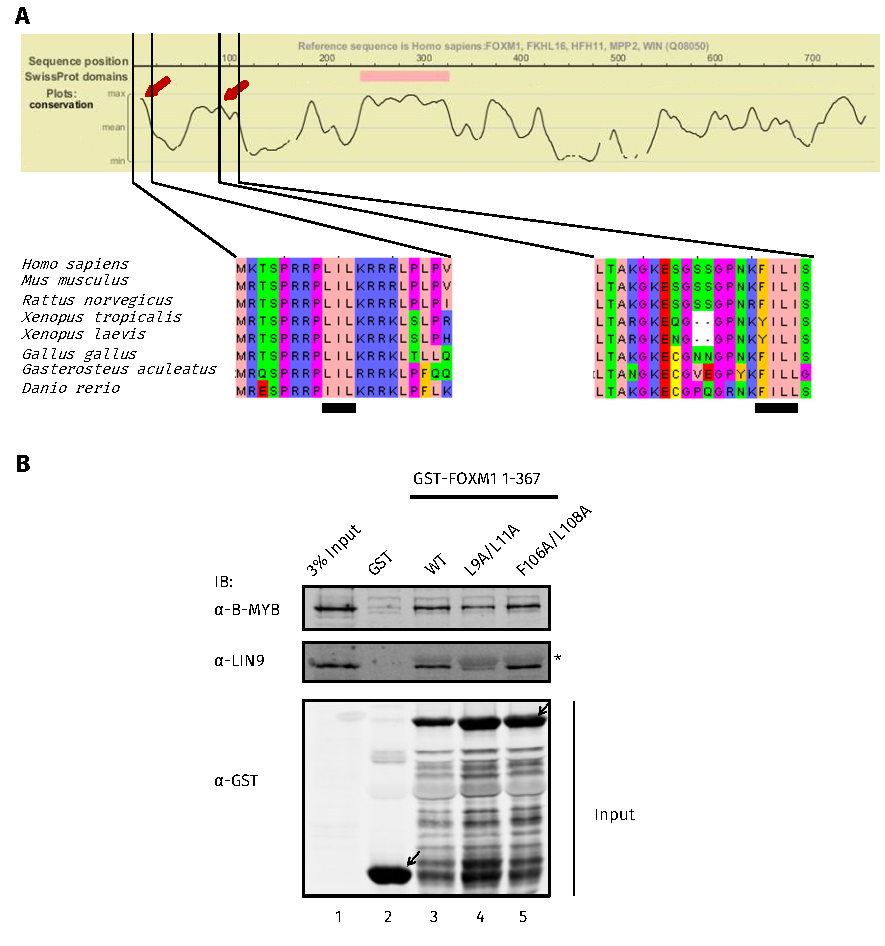
\includegraphics[width=0.9\textwidth]{chapter3/figures_foxm1/fig33.pdf}
    \caption[Identification of the amino acids in FOXM1 that are responsible for the MMB interaction]{\textbf{Identification of the amino acids in FOXM1 that are responsible for the MMB interaction. (A) Top,} profile of regional evolutionary conservation along the protein. Red arrows indicate the two highly conserved regions within amino acids 1 - 116. Pink bar indicates the position of the Forkhead DNA-binding domain according to the SwissProt domains database. \textbf{Bottom,}  sequence alignment of the indicated regions from different species. Colour theme Zappo in jalview was used to mark the different amino acids. The hydrophobic regions were marked by the black bars below. \textbf{(B)} GST pulldown assays using the wild-type or indicated mutant FOXM1 GST fusion proteins with U2OS cell lysates. \textasciitilde 1 $\mu$g of purified protein was used per pulldown. After washing, the pulldowns was immunoblotted (IB) with the indicated antibodies. The $\alpha$-GST blot showed relatively equal loading of GST and GST-tagged FOXM1 truncations (black arrows) used in the pulldown assays. Asterisk indicates the location of a cross-reacting band with the LIN9 antibody arising from the GST fusion protein.}
    \label{fig:fig33}
\end{figure}

To test whether this is the case, the leucines and phenylalanines within each of these regions were mutated to alanines (L9A/L11A, and F106A/L108A). The abilities of these two mutants to interact with the MMB complex were investigated using a GST pulldown assay. The F106A/L108A mutant was able to bind B-MYB and LIN9 to a similar level as observed with the wild-type FOXM1 (\textbf{Figure \ref{fig:fig33}B}, lanes 3 and 5). However, the interaction between the L9A/L11A mutant and B-MYB and LIN9 was significantly weaker than the wild-type FOXM1 (\textbf{Figure \ref{fig:fig33}B}, lanes 3 and 4), indicating these two leucines (Leu9 and Leu11) are important for the MMB interaction. Interestingly, similar to the $\Delta$1-116 truncation, the effect of the L9A/L11A mutations on the interaction with LIN9 was more apparent.

Given that the Leu9 and Leu11 are important for FOXM1 to interact with the MMB complex \textit{in vitro}, we next tested whether mutation of these two amino acids will affect the binding of FOXM1 to the MMB complex \textit{in vivo}. To this end, a triple FLAG-tagged full-length FOXM1 protein which bears the L9A/L11A mutations was generated. Co-immunoprecipitation experiments were performed in U2OS cells after the transfection of the wild-type or the mutant construct using an anti-FLAG antibody. The N-terminal truncated FOXM1 ($\Delta$1-116) was also included for comparison. Consistent with the GST pulldown assay, mutations of L9A/L11A significantly reduced the binding of FOXM1 to B-MYB and LIN9, although some background binding to B-MYB was observed, indicating the dynamic range of the IP is poor (\textbf{Figure \ref{fig:fig34}A}, lane 5). The effect of the mutations on the interaction with LIN9 was more prominent as no detectable LIN9 binding was observed with the FOXM1 L9A/L11A protein (\textbf{Figure \ref{fig:fig34}A}, middle panel, lane 7).

\begin{figure}[!h]
    \centering
    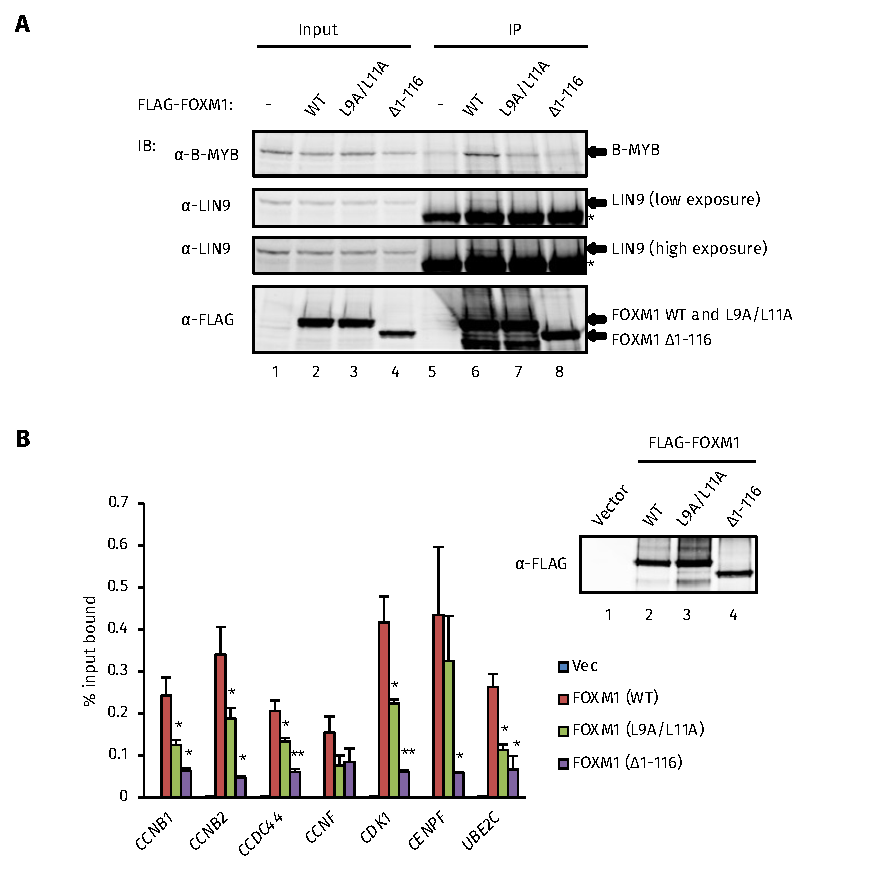
\includegraphics[width=0.85\textwidth]{chapter3/figures_foxm1/fig34.pdf}
    \caption[The two amino acids Leu9 and Leu11 at the N-terminus of FOXM1 are important for its interaction with the MMB complex and its recruitment to DNA]{\textbf{The two amino acids Leu9 and Leu11 at the N-terminus of FOXM1 are important for its interaction with the MMB complex and its recruitment to DNA. (A)} Co-immunoprecipitation of the FOXM1 (WT), FOXM1 (L9A/L11A) and FOXM1 ($\Delta$1-116) proteins with B-MYB and LIN9. The indicated FOXM1 protein constructs were transfected into U2OS cells, and associated protein complexes were precipitated with an anti-FLAG antibody and Protein G Dynabeads. Immunoprecipitated proteins were detected (IB) with the indicated antibodies. Two different exposures of the $\alpha$-LIN9 blot are shown. The asterisk indicates the heavy chain of IgG. \textbf{(B)} ChIP analyses of the binding of FOXM1 (WT), FOXM1 (L9A/L11A) and FOXM1 ($\Delta$1-116) at the indicated loci. HEK293T cells were transfected with plasmids encoding the indicated proteins, and ChIP experiments were performed using an anti-FLAG antibody. Expression levels of the proteins were tested by western blot with an anti-FLAG antibody (right). Error bars represent the standard deviation from two independent experiments. The P-value was calculated using a t-test. * and ** represent $P<0.05$ and $P<0.01$, respectively.}
    \label{fig:fig34}
\end{figure}

Having confirmed that the mutations of the Leu9 and Leu11 amino acids also affect the binding of FOXM1 to the MMB complex in vivo, we next tested the \textit{in vivo} chromatin binding ability of this mutant. Plasmids encoding the wild-type or the L9A/L11A mutant FOXM1 with a triple FLAG tag were transfected into HEK293T cells, ChIP experiments were performed using an anti-FLAG antibody. The N-terminal truncated FOXM1 ($\Delta$1-116) was also included in the experiments as a comparison. The expression levels of different versions of FOXM1 protein were very similar (\textbf{Figure \ref{fig:fig34}B}). Consistent with previous results, the recruitment of the FOXM1 (L9A/L11A) mutant to chromatin was significantly reduced at a number of tested regions (\textbf{Figure \ref{fig:fig34}B}). The N-terminal truncated FOXM1 ($\Delta$1-116) affected the chromatin binding to a greater extent than the L9A/L11A mutant did (\textbf{Figure \ref{fig:fig34}B}), indicating there might be other amino acids in this regions which also contribute the chromatin binding of FOXM1. Of note, the effect of either the L9A/L11A mutations or the $\Delta$1-116 N-terminal truncation on the FOXM1 binding at the \textit{CCNF} locus was only marginal (\textbf{Figure \ref{fig:fig34}B}), which is consistent with previous results (\textbf{Figure \ref{fig:fig32}C}).

In summary, the N-terminal domain (aa 1-116) of FOXM1 is critical for its interaction with the MMB complex both \textit{in vitro} and \textit{in vivo}. More importantly, it is also important for the chromatin recruitment of FOXM1. The Leu9 and Leu11 amino acids within this domain are essential for the interaction with the MMB complex and partially contribute to the chromatin recruitment of FOXM1.

\subsection{The N-terminus of FOXM1 is a multifunctional domain}

Given that the N-terminal domain of FOXM1 is critical for its interaction with the MMB complex and its DNA binding, we next investigated the transcriptional activities of the mutated (L9A/L11A) and truncated ($\Delta$1-116) forms of FOXM1.

To this end, luciferase assays were performed using the reporter driven by the \textit{CCNB1} or \textit{CCNB2} promoter sequences. A reporter driven by six tandem canonical Forkhead consensus (6$\times$FOX) (\cite{samadani1996the}) was also included in the experiment for comparison.

Since the chromatin recruitment of both L9A/L11A mutated and the $\Delta$1-116 truncated FOXM1 was undermined on \textit{CCNB1} and \textit{CCNB2} promoters (\textbf{Figure \ref{fig:fig34}B}), we expected to observe reduced activation of these two forms of FOXM1 comparing to the wild-type protein. However, while the wild-type FOXM1 protein only weakly activated the tested reporters, the FOXM1 L9A/L11A mutant possessed some repressive effect on all the reporters tested, most prominently on the \textit{CCNB1} reporter (\textbf{Figure \ref{fig:fig35}A} and \textbf{B}), indicating this mutant might act as a dominant-negative form of FOXM1. This implies that the Leu9 and Leu11 amino acids are also important for the FOXM1 transcriptional activity.

\begin{figure}[!h]
    \centering
    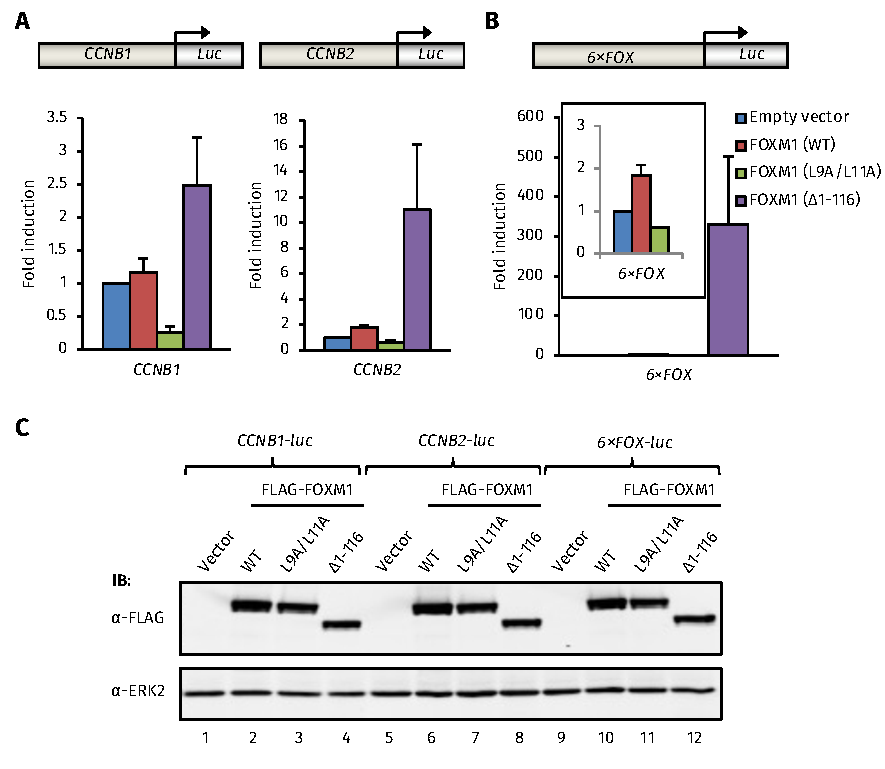
\includegraphics[width=0.9\textwidth]{chapter3/figures_foxm1/fig35.pdf}
    \caption[Transcriptional activities of mutant FOXM1 proteins]{\textbf{Transcriptional activities of mutant FOXM1 proteins. (A)} Luciferase assays after the overexpression of the indicated FOXM1 proteins. The activities of luciferase driven by the \textit{CCNB1} and \textit{CCNB2} promoters were normalised by the protein concentrations of the extracts. Error bars represent the standard deviation from two independent experiments. \textbf{(B)} The same experiment performed in \textbf{(A)} on the 6$\times$FOX reporter luciferase. Error bars represent the standard deviation from two independent experiments. \textbf{(C)} Western blot checking the expression level of different FLAG-tagged FOXM1 proteins used in the luciferase experiments in \textbf{(A)} and \textbf{(B)}. The extracts were immunoblotted (IB) with the indicated antibodies. The ERK2 antibody was used as a loading control.}
    \label{fig:fig35}
\end{figure}

In contrast, the FOXM1 ($\Delta$1-116) truncation was significantly more active than the wild- type FOXM1 (\textbf{Figure \ref{fig:fig35}A} and \textbf{B}). Previous studies have suggested that the N-terminal domain of FOXM1 served as an auto-inhibitory domain to keep FOXM1 inactive at G1 phase (\cite{laoukili2008activation,park2008an}). Therefore, although FOXM1 ($\Delta$1-116) has lower occupancy at the promoter of \textit{CCNB1} and \textit{CCNB2} than the wild-type FOXM1, it holds much higher activity, which partially explains the stronger induction of FOXM1 ($\Delta$1-116) on the \textit{CCNB1} and \textit{CCNB2} reporters.

Intriguingly, the transactivation effect of FOXM1 ($\Delta$1-116) on the 6$\times$FOX reporter was much more dramatic than that on \textit{CCNB1} and \textit{CCNB2} reporters. The \textit{CCNB1} and \textit{CCNB2} reporters were only moderately induced by the FOXM1 ($\Delta$1-116) (\textasciitilde 2 - 12 fold) (\textbf{Figure \ref{fig:fig35}A}), but the 6$\times$FOX reporter was activated by several hundred fold (\textbf{Figure \ref{fig:fig35}B}). The difference of the reporter activities were not due to the different expression levels of the tested FOXM1 proteins, because western blot analyses showed that they were expressed at the similar level. These results indicate that the mechanisms by which FOXM1 activates these promoters are different.

In summary, the N-terminal domain of FOXM1 serves as a multifunctional domain. First, it is important for MMB binding and the chromatin recruitment of FOXM1. Second, it is also an auto-inhibitory domain to repress the FOXM1 transcriptional activity. Third, the Leu9 and the Leu11 residues within this domain are required for FOXM1 transcriptional activity.

\subsection{An intact DNA-binding domain is required for the chromatin recruitment of FOXM1}

To further substantiate our hypothesis that FOXM1 is indirectly recruited to the CHR motif by the MMB complex, we used the FOXM1 (R286A/H287A) mutant to test the binding at FOXM1 target genes. This mutant is incapable of DNA binding as predicted by the structure (\cite{littler2010structure}) but is able to be recruited to the \underline{W}nt \underline{r}esponse DNA \underline{e}lement (WRE) by $\beta$-catenin (\cite{zhang2011foxm1}). If FOXM1 is indirectly recruited to the CHR motif by the MMB complex, just as it is indirectly recruited to the WRE by $\beta$-catenin (\cite{zhang2011foxm1}), the binding of FOXM1 R286A/H287A mutant should have a similar occupancy as the wild-type FOXM1 on the CHR containing regions.

To check whether this is the case, first, immunofluorescence experiments were performed to confirm that the R286A and H287A mutations did not alter the nuclear localisation of FOXM1. Consistent with previous research, the FOXM1 (R286A/H287A) was mainly in the nucleus, just like the wild-type FOXM1 (\textbf{Figure \ref{fig:fig36}A}) (\cite{zhang2011foxm1}). Then, ChIP experiments were performed in HEK293T cells after the transfection of triple FLAG- tagged wild-type or R286A/H287A mutant versions of FOXM1. The N-terminal truncated FOXM1 ($\Delta$1-116) was also included as a comparison. The expression levels of three different versions of FOXM1 protein were very similar (\textbf{Figure \ref{fig:fig36}B}, right panel).

\begin{figure}[!h]
    \centering
    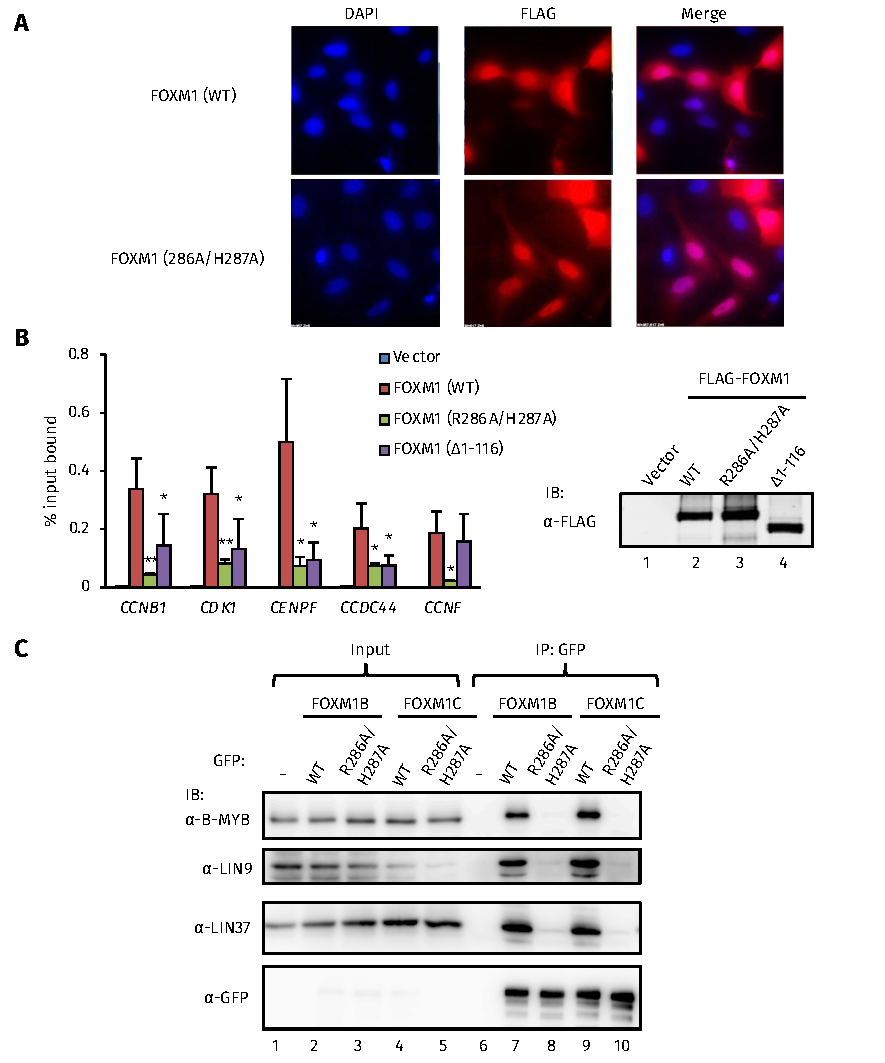
\includegraphics[width=0.9\textwidth]{chapter3/figures_foxm1/fig36.pdf}
    \caption[The R286A and H287A mutations affect FOXM1 chromatin binding and its interactions with the MMB complex]{\textbf{The R286A and H287A mutations affect FOXM1 chromatin binding and its interactions with the MMB complex. (A)} Immunofluorescence analyses showing the localisation of the wild-type FOXM1 (WT) and FOXM1 (R286A/H287A) proteins. U2OS cells were transfected with the indicated constructs. Cells were incubated with FLAG antibody, and the signals were visualised by the Alexa Fluor 594-conjugated anti-mouse secondary antibody (red). DNA was stained with DAPI (blue). \textbf{(B)} ChIP analyses of the binding of FOXM1 (WT) and FOXM1 (R286A/H287A) at the indicated loci. HEK293T cells were transfected with plasmids encoding the indicated proteins, and ChIP experiments were done using an anti-FLAG antibody. Expression levels of the proteins were tested by western blot (IB) with an anti-FLAG antibody. Error bars represent the standard deviation from two independent experiments. P- values were calculated using a t-test. * and ** represents $P<0.05$ and $P<0.01$ respectively. \textbf{(C)} Co- immunoprecipitation of the FOXM1 WT and FOXM1 R286A/H287A proteins with B-MYB and LIN9. The indicated FOXM1 protein constructs were transfected into HEK293 cells, and associated protein complexes were precipitated with a GFP antibody. The co-immunoprecipitated proteins were detected (IB) with indicated antibodies.}
    \label{fig:fig36}
\end{figure}

Surprisingly, the binding signals of the FOXM1 (R286A/H287A) mutant was significantly curtailed comparing to the wild-type FOXM1 in all tested regions, and in some cases its binding was even lower than the FOXM1 ($\Delta$1-116) (\textbf{Figure \ref{fig:fig36}B}). Although the occupancy of the FOXM1 ($\Delta$1-116) at the \textit{CCNF} locus was comparable to that of the wild-type protein, the FOXM1 (R286A/H287A) binding level was drastically reduced at the \textit{CCNF} locus (\textbf{Figure \ref{fig:fig36}B}). This implies that the reasons leading to the reduced binding of FOXM1 ($\Delta$1-116) and FOXM1 (R286A/H287A) are different. More intriguingly, co-immunoprecipitation using GFP-tagged FOXM1B or FOXM1C bearing the R286A/H287A mutations demonstrated that these two point mutations completely abolished the interaction between FOXM1 and the MMB complex \textit{in vivo} (\textbf{Figure \ref{fig:fig36}C}, lanes 8 and 10). This contrasts with the observation that the R286A/H287A mutations did not affect the binding of FOXM1 to the MMB complex in vitro as shown from the GST pulldown experiments (\textbf{Figure \ref{fig:fig31}B}).

Therefore, an intact DNA-binding domain is needed for both the chromatin recruitment of FOXM1 and its interaction with the MMB complex \textit{in vivo}.

To further investigate the transcriptional activity of the FOXM1 (R286A/H287A) mutant, luciferase assays were carried on to test its activity on reporters driven by the \textit{CCNB1} and \textit{CCNB2} promoters or the 6$\times$FOX sequence. The expression levels of FOXM1 (WT) and FOXM1 (R286A/H287A) were very similar (\textbf{Figure \ref{fig:fig37}C}). Although the level of FOXM1 ($\Delta$1-116) was slightly lower than the other two versions of FOXM1 (\textbf{Figure \ref{fig:fig37}C}), its transcriptional activity was still the highest (\textbf{Figure \ref{fig:fig37}A} and \textbf{B}). Consistent with the ChIP experiments where the binding of the FOXM1 (R286A/H287A) was significantly diminished, FOXM1 (R286A/H287A) failed to activate all three reporters tested (\textbf{Figure \ref{fig:fig37}A} and \textbf{B}). In addition, FOXM1 (R286A/H287A) also had some repressive effect which is similar to FOXM1 (L9A/L11A) (\textbf{Figure \ref{fig:fig37}A} and \textbf{B}), which indicated that FOXM1 (R286A/H287A) might also act as a dominant-negative form of FOXM1.

\begin{figure}[!h]
    \centering
    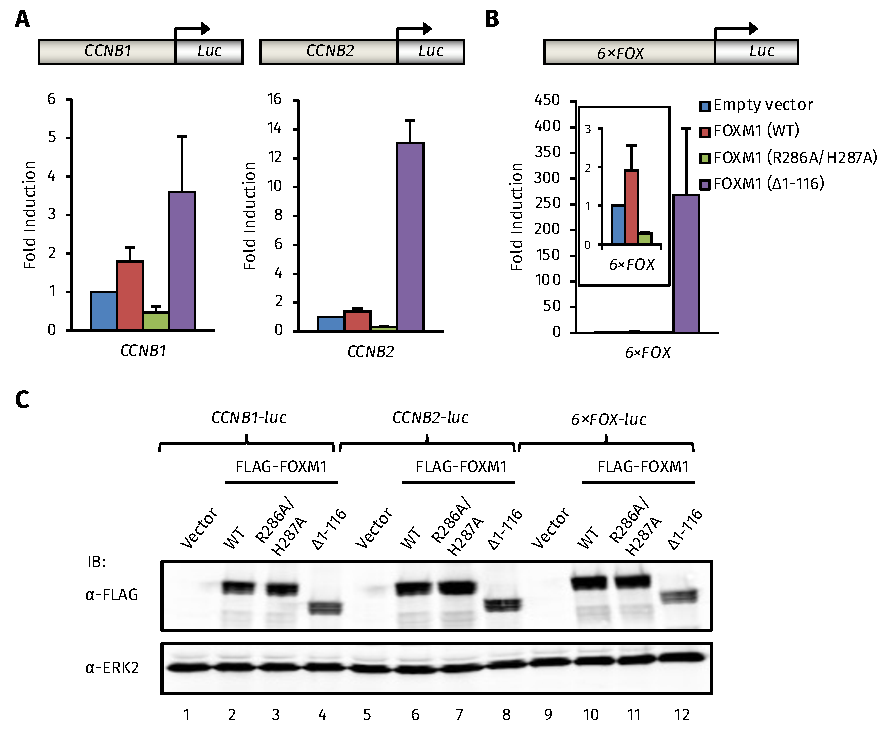
\includegraphics[width=0.9\textwidth]{chapter3/figures_foxm1/fig37.pdf}
    \caption[Transcriptional activities of the FOXM1 (R286A/H287A) mutant]{\textbf{Transcriptional activities of the FOXM1 (R286A/H287A) mutant. (A)} Luciferase assays after the overexpression of the indicated FOXM1 proteins. The activities of luciferase driven by the \textit{CCNB1} and \textit{CCNB2} promoters were normalised by the protein concentrations. Error bars present the standard deviation from two independent experiments. \textbf{(B)} The same experiment performed in \textbf{(A)} on the 6$\times$FOX luciferase reporter. Error bars represent the standard deviation from two independent experiments. \textbf{(C)} Western blot checking the expression level of different FLAG-tagged FOXM1 proteins used in the luciferase experiments in \textbf{(A)} and \textbf{(B)}. The extracts were immunoblotted (IB) with the indicated antibodies. The ERK2 antibody was used as a loading control.}
    \label{fig:fig37}
\end{figure}

Therefore, it seems both protein-protein interactions and potential protein-DNA interactions are needed for the recruitment of FOXM1 to chromatin.

In summary, the Arg286 and His287 amino acids within the DNA-binding domain of FOXM1 are two critical residues for the functions of FOXM1. They are required for: \textbf{1)} the specific interaction with the Forkhead consensus (\cite{littler2010structure}); \textbf{2)} the interaction with the MMB complex \textit{in vivo}; \textbf{3)} the chromatin recruitment of FOXM1; \textbf{4)} the transcriptional activity of FOXM1.

\subsection{Summary}

Collectively, the data presented in this section describe a detailed analysis of the FOXM1 cistrome. Two independent FOXM1 ChIP-seq experiments were performed, and 270 peaks which came out from both experiments were preserved as high confidence FOXM1 binding events. A lot of previously-established FOXM1 target genes, especially those well- characterised G2/M target genes of FOXM1, are present in the dataset. Some known target genes, such as \textit{CKS1B} and \textit{BIRC5}  fail to be identified from the ChIP-seq experiments, presumably due to low enrichment bindings which are often below the threshold of detection in a high-throughput experiment. Indeed, we can reproducibly detect enrichment of FOXM1 on \textit{CKS1B} and \textit{BIRC5} promoters by ChIP-qPCR, but the signals are generally lower than those at the 270 ChIP-seq derived peaks (\textbf{Figure \ref{fig:fig17}C} and data not shown).

Gene ontology analysis on the 270 FOXM1 peaks resulted in 91 enriched biological processes, most of which are related to cell cycle regulation, especially M phase. Only a few enriched terms are not directly related to the cell cycle control. Such specificity on cell cycle regulation is quite unexpected, although FOXM1 is a well-known cell cycle regulator. In agreement with the gene ontology analysis, most of the FOXM1-bound genes exhibit some cyclic expression pattern throughout the cell cycle, with the majority of them peaking at M phase. It is interesting to note that upon the knockdown of FOXM1, the changes of the expression levels of its target genes are only modest. The effects of FOXM1 depletion on the expressions of \textit{CCNB1} and \textit{CCNF} were the most prominent (\textasciitilde 50\% reduction), but the other target genes only marginally (10-20\% reduction) respond to the FOXM1 knockdown. However, though modest, almost all tested genes showed reduced expression after the FOXM1 depletion (\textbf{Figure \ref{fig:fig21}}). This \enquote{modest but broad} effect is consistent with the notion that FOXM1 is a master regulator of the mitotic genes (\cite{laoukili2005foxm1,lefebvre2010a}). By the depletion of FOXM1, although the change of individual mitotic genes is modest, a large array of mitotic genes is affected. Therefore, the overall effect could be catastrophic.

A lot of known target genes were identified from the ChIP-seq analysis, but the FOXM1- binding regions at those genes are quite surprising. It was generally believed that FOXM1 binds to the canonical Forkhead consensus located in the promoters of these target genes (\cite{wang2005forkhead}), but our ChIP-seq data clearly suggest that is not the case. Instead, most FOXM1 peaks are within the core promoters of its target genes where the CHR motif is located. This finding has been confirmed by ChIP-qPCR using promoter walking and siRNA against FOXM1.

Motif analysis revealed that the CHR motif and the CCAAT-box motif, not the canonical Forkhead DNA motif, are enriched within FOXM1 peaks. Indeed, only 25 FOXM1 peaks contain the FOXM1 in vitro binding site TAAACA, which is the same as the occurrence of this motif in randomly selected background sequences (25 peaks out of 270). However, \textit{in vitro} bandshift experiments using the purified FOXM1 DNA-binding domain demonstrate that FOXM1 does not directly bind to the CHR motif, at least not with a high enough affinity to be detected using this technique. It still specifically binds to the canonical Forkhead consensus at an extremely low affinity (at least one order of magnitude lower than FOXK2 and FOXO3 DNA-binding domains). The enrichment of the CHR motif and the CCAAT-box motif within the FOXM1 peaks implies that the MMB/DREAM complex and the transcription factor NF-Y may contribute to the DNA recruitment of FOXM1. Co-immunoprecipitation experiments suggest that FOXM1 interacts with the MMB complex, but not the DREAM complex or NF-Y. Consistent with this finding, knockdown of DREAM-specific components or NF-YA do not affect the DNA binding of FOXM1.

Both the CHR motif and the MMB complex are critical for the recruitment of FOXM1 to chromatin. Mutation of the CHR motif in the promoter results in significantly reduced binding and failed activation by FOXM1. Interestingly, the biotinylated DNA pulldown assay suggests that FOXM1 bind to the naked DNA containing the CHR motif at a non- specific binding level. It is possible that the proper genomic context is important for the recruitment of FOXM1 to DNA. This hypothesis is partly supported by the evidence that the binding of FOXM1 to a luciferase transgene bearing the wild-type \textit{CCNB2} promoter sequence is much lower than its binding at the endogenous \textit{CCNB2} locus (data not shown).

Knockdown of LIN9 and B-MYB lead to a reduced promoter-binding signal of FOXM1, indicating that the interaction with the MMB complex is important for the recruitment of FOXM1 to chromatin. Intriguingly, a recent study indicates that the interaction between FOXM1 and the MMB complex happens at early G1 phase and throughout the cell cycle (\cite{sadasivam2012the}). Consistent with this finding, our ChIP experiments showed that FOXM1 was loaded on to the promoters as early as in G1 phase, and the promoter-binding of FOXM1 remain relatively constant throughout the cell cycle (\textbf{Figure \ref{fig:fig17}C}). This allows the cell cycle kinases to regulate a pre-assembled complex on the promoter, leading to rapid activation of the genes at the G2 and M phases (see the model proposed at the end of this section).

Since physical interaction between FOXM1 and the MMB complex can be detected both \textit{in vitro} and \textit{in vivo}, it is not surprising that the majority of FOXM1 binding events are shared with LIN9/B-MYB. Although FOXM1 has its own specific binding regions, the average signals at the FOXM1-specific peaks are generally lower than that of those which are shared by LIN9/B-MYB. This indicates that LIN9/B-MYB could stabilise FOXM1 chromatin binding. On the other hand, the higher occupancy might be simply because FOXM1 is more easily immunoprecipitated (epitope more exposed to the antibody \textit{etc.}) when co-bind with LIN9/B-MYB. Interestingly, within the FOXM1-specific binding sites which lack apparent MMB complex binding \textit{in vivo}, 47\% of them also contain the CHR motif (\textbf{Figure \ref{fig:fig29}B}). It is unclear about the functions of these CHR motifs, and we are unable to conclude whether these FOXM1-specific peaks are really independent of LIN9/B-MYB due to the lack of ChIP-seq data for LIN9/B-MYB in the cell line we used (U2OS).

The MMB complex interaction regions in FOXM1 were mapped to the N-terminal domain (aa 1-116) and the Forkhead DNA-binding domain of FOXM1. Both domains are required for the interaction with the MMB complex \textit{in vitro}. Although no evidence suggests the N- terminal domain contacts DNA so far, deletion of this domain causes a reduced occupancy of FOXM1 on most of its target genes, presumably due to the compromised ability of interacting with the MMB complex. In addition, the N-terminal domain is an auto- inhibitory domain, and deletion of this part generates a hyperactive form of FOXM1. Within this inhibitory region, there are two amino acid residues Leu9 and Leu11 which are also important for both interaction with the MMB complex and the transcriptional activity of FOXM1. Deletion of aa 1-116 resulted in the loss of interaction with the MMB complex and the hyperactivation of FOXM1 transcriptional activity; mutations of Leu9 and Leu11 resulted in the loss of interaction with the MMB complex and the loss of transcriptional activity as well. These findings indicate that, within the N-terminal domain, the amino acids contribute to the MMB complex interaction are different from those that are responsible for the auto-inhibitory effect. Interestingly, the LXL sequence was shown to be able to recruit Cyclin-Cdk complexes just as efficiently as the traditional Cy (RXL) motif (\cite{wohlschlegel2001mutational}). It is possible that the mutations of these two leucines disrupt the binding between FOXM1 and Cyclin-Cdk complexes which are important for the transcriptional activity of FOXM1 (\cite{wang2005forkhead,fu2008plk1-dependent}). Indeed, two LXL motifs at the C-terminus of FOXM1 have already been shown to be important for the binding of Cyclin-Cdk complex (\cite{wang2005forkhead,laoukili2008activation}).

The mutations of R286A/H287A within the FOXM1 DNA-binding domain also provide a lot of intriguing information. The structure of the FOXM1 DNA-binding domain predicts that these two mutations will only compromise the specific interaction between FOXM1 and the Forkhead canonical DNA motif (\cite{littler2010structure}). However, the FOXM1 R286A/H287A mutant fails to bind the promoters of its target genes where the CHR motif, not the canonical Forkhead DNA motif, is located. On the other hand, co- immunoprecipitation experiments demonstrate the FOXM1 (R286A/H287A) is, for some unknown reasons, unable to interact with the MMB complex \textit{in vivo}, even though GST pulldown assays suggest the R286A/H287A mutations do not affect the interaction between FOXM1 and the MMB complex \textit{in vitro}. Therefore, it is difficult to draw the conclusion whether the loss of \textit{in vivo} DNA binding of FOXM1 R286A/H287A mutant is a cause or a consequence of its loss of interaction with the MMB complex. Based on the co-immunoprecipitation and GST pulldown experiments in the presence of ethidium bromide, the interaction between FOXM1 and the MMB complex is independent of the DNA. Hence, it is tempting to speculate the loss of DNA binding of the FOXM1 R286A/H287A mutant is due to its inability to interact with the MMB complex \textit{in vivo}.

Another interesting discovery is the \textit{in vivo} chromatin binding of FOXM1 to the \textit{CCNF} promoter region. A functional CHR motif has been identified around the TSS of \textit{CCNF} (Müller and Engeland, unpublished data). However, none of LIN9, B-MYB, and FOXM1 binds to the region containing this motif \textit{in vivo}. LIN9 and B-MYB do not bind to the \textit{CCNF} locus in HeLa cells (\cite{sadasivam2012the}), while FOXM1 binds to the upstream promoter of \textit{CCNF} (-298 bp relative to the TSS), where neither the CHR motif nor the Forkhead motif is present. Importantly, the binding of FOXM1 to this locus is independent of the MMB complex, and its DNA-binding domain is required for the recruitment to this locus. This implies that at a subset of its binding sites, at least at the \textit{CCNF} locus, some protein-DNA interactions are needed. It will be interesting to look at whether there are some other FOXM1 binding sites like the \textit{CCNF} locus, which might reveal a different mechanism for the chromatin recruitment of FOXM1.

Based on the data presented in this section and other studies (\cite{park2008anaphase-promoting,alvarez-fernández2011protein,müller2012the,sadasivam2012the}), we are able to propose a model for the regulation of the G2 and M phases by a novel cell cycle regulatory complex which consists of the MMB complex and the Forkhead transcription factor FOXM1 (\textbf{Figure \ref{fig:fig38}}): in quiescent cells, the DREAM complex keeps the genes whose activities peak at the G2 and M phases repressed via the CHR motif; when cells enter the G1 phase, the DREAM complex disassembles and the MuvB core forms a new complex with the transcription factors B-MYB (the MMB complex) and FOXM1; at this stage, the MMB/FOXM1 complex is already loaded on to the promoter of the gene, but the transcriptional activity of this complex is low; as the cell cycle proceeds, several cell cycle kinases (Cyclin-Cdk, PLK1 \textit{etc.}) phosphorylate B-MYB and FOXM1, leading to the degradation of B-MYB and a hyperactivation of FOXM1 which subsequently activate the transcription of the gene; when cells exit mitosis, other cell cycle regulatory proteins (APC/C, B55$\alpha$, \textit{etc.}) cause the degradation and de-phosphorylation of FOXM1 which results in reduced transcription of its target genes.

The regulatory roles of the MMB complex and FOXM1 on the G2-M transition were discovered separately and now have finally converged as a result of our studies and others (\cite{down2012binding,müller2012the,sadasivam2012the}).

\begin{figure}[!h]
    \centering
    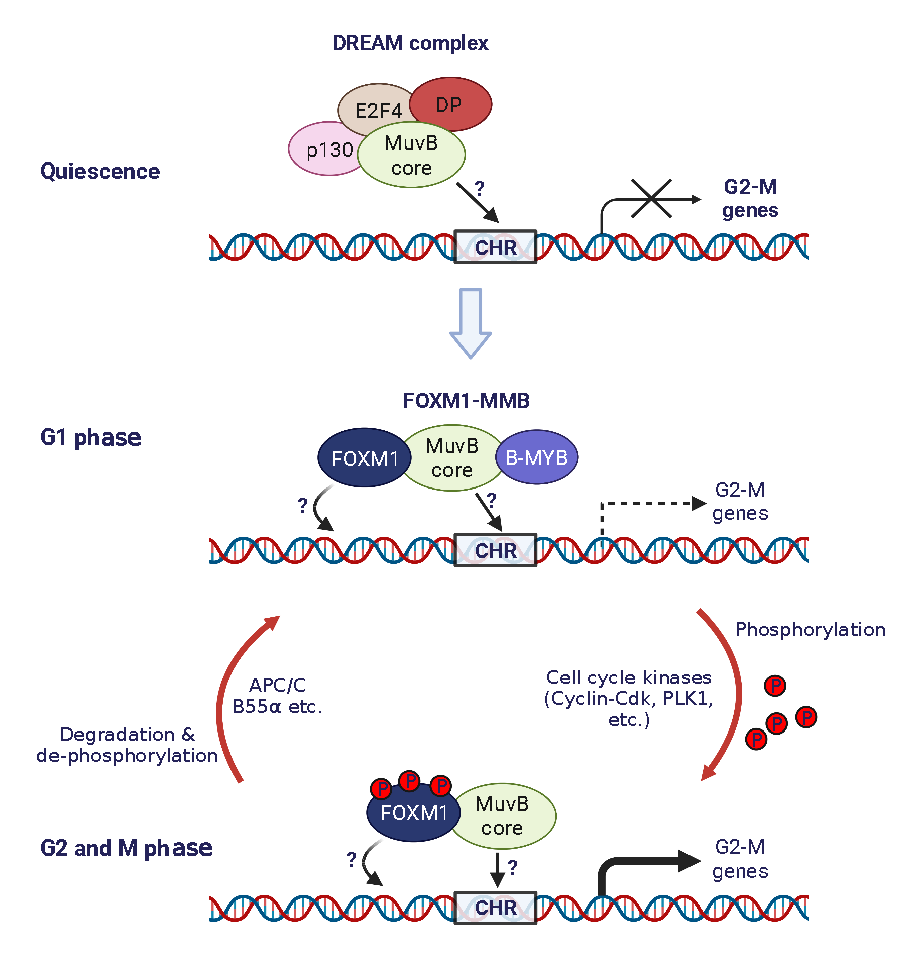
\includegraphics[width=0.85\textwidth]{chapter3/figures_foxm1/fig38.pdf}
    \caption[Model proposed for the cell cycle regulation by different protein complexes]{\textbf{Model proposed for the cell cycle regulation by different protein complexes.} The red Ps represent phosphorylation events. The question marks represent the uncertainty of DNA contacts. See more detailed description in the main text.}
    \label{fig:fig38}
\end{figure}


\section{FOXO3 and FOXK2 bind to both overlapping and specific genomic regions}\label{section:foxo3}

\subsection{Validation of FOXO3 ChIP-seq data}

After the discovery that FOXM1gains its own specific binding events by protein-protein interactions with the MMB complex, we next investigated the DNA-binding specificity of two other typical Forkhead proteins: FOXO3 and FOXK2, both of which bind to the canonical Forkhead consensus and are linked to the cell cycle control.

\begin{figure}[!h]
    \centering
    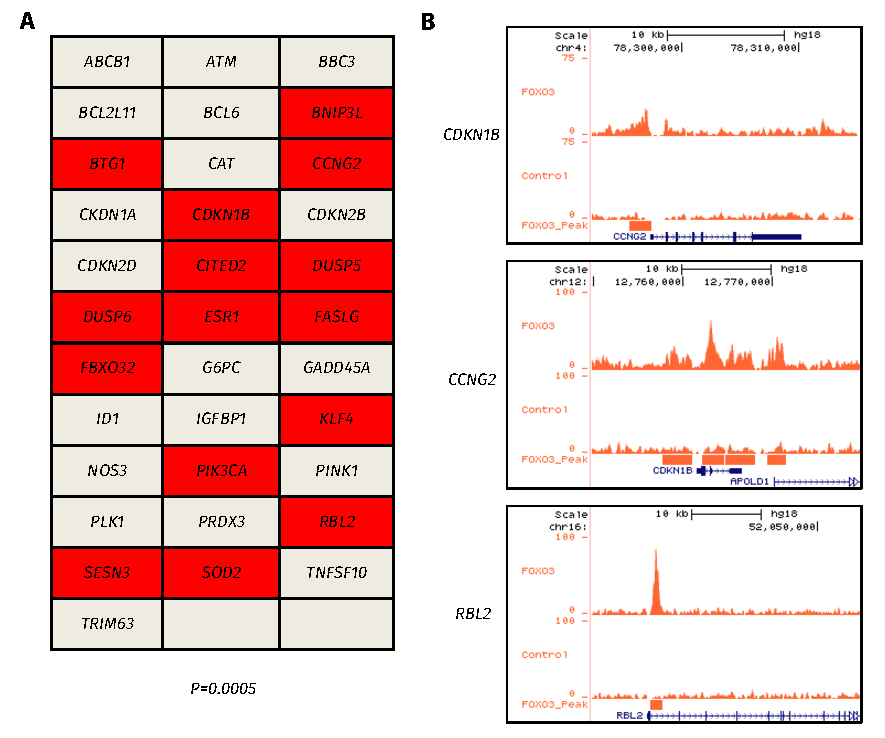
\includegraphics[width=0.9\textwidth]{chapter3/figures_foxo3/fig39.pdf}
    \caption[FOXO3 binding at known target genes]{\textbf{FOXO3 binding at known target genes. (A)} 34 known target genes of FOXO3 according to the transcription factor encyclopaedia (\cite{yusuf2012the}). Red colour indicates the genes that are also identified by the FOXO3 ChIP-seq experiment. The P-value was calculated by a Fisher's exact test. \textbf{(B)} Snapshots of FOXO3 peak profiles at the \textit{CCNG2}, \textit{CDKN1B}, \textit{RBL2} loci.}
    \label{fig:fig39}
\end{figure}

To confirm the reliability of the FOXO3 ChIP-seq experiment, we first checked whether the previously-discovered FOXO3 target genes were actually bound by FOXO3 in the ChIP-seq dataset. Among the 34 manually-curated target genes in The Transcription Factor Encyclopaedia (\cite{yusuf2012the}), 15 of them were bound by FOXO3 (\textbf{Figure \ref{fig:fig39}A}). These include the well-known cell cycle arrest regulators \textit{CCNG2}, \textit{CDKN1B} (\textit{p27}), and \textit{RBL2} (\textit{p130}) (\textbf{Figure \ref{fig:fig39}A} and \textbf{B}). Interestingly, unlike the FOXM1 peaks which are mainly located within the core promoter of its target gene, the locations of FOXO3 peaks around its target genes were quite variable: some were in the promoter region (\textit{e.g. CCNG2}); some were in the gene body (coding exons and introns) (\textit{e.g. RBL2}); some were present in both the promoter and the gene body (\textit{CDKN1B}) (\textbf{Figure \ref{fig:fig39}B}).

Having confirmed that many known FOXO3 target genes are present in the FOXO3 ChIP- seq data, we next started to experimentally validate the ChIP-seq derived FOXO3 peaks. To this end, we randomly selected twelve peaks with varying enrichments from the ChIP-seq data and tested the FOXO3 binding at these loci. ChIP experiments were performed in the U2OS-FOXO3 stable cell line after the treatment with LY294002 to induce FOXO3 nuclear entry and doxycycline to induce FOXO3 expression using the FLAG antibody. All tested regions showed more than 10 fold enrichment over the control ChIP experiments performed in the U2OS T-REX host cell line (\textbf{Figure \ref{fig:fig40}A}). The binding at each locus, as represented by \% input bound, was also positively correlated with the ChIP-seq signal, as represented by the tag density, \textit{i.e.} regions with higher \% input bound tend to have higher tag density according to the ChIP-seq, although this relationship was not linear $R^2=0.48$ (\textbf{Figure \ref{fig:fig40}B}). In addition, the \textit{CCNB1} and \textit{PLK1} promoter regions, where FOXM1 peaks are located, were also included in the experiments as negative control regions. No significant enrichment was detected on either locus (\textbf{Figure \ref{fig:fig40}A}).

\begin{figure}[!h]
    \centering
    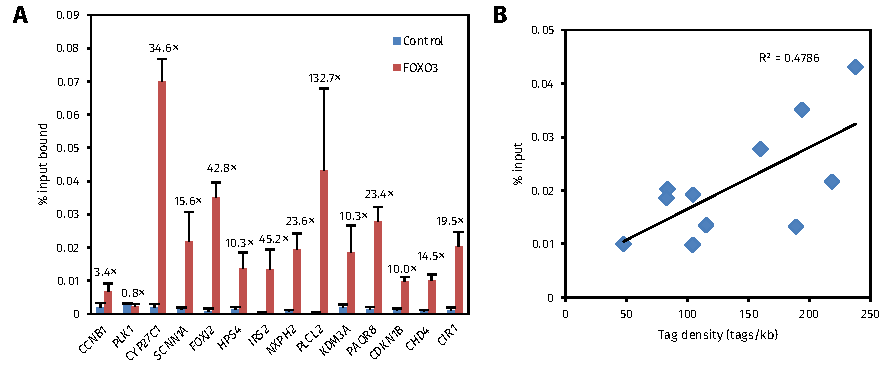
\includegraphics[width=0.9\textwidth]{chapter3/figures_foxo3/fig40.pdf}
    \caption[ChIP-qPCR validation on selected FOXO3 peaks]{\textbf{ChIP-qPCR validation on selected FOXO3 peaks. (A)} Twelve randomly selected FOXO3 peaks with various enrichment levels were tested using ChIP-qPCR. ChIP experiments were performed using a FLAG antibody on the U2OS-FOXO3 stable cell line after 24 hours treatment with doxycycline and 2 hours treatment with LY294002. Fold enrichment over a control ChIP experiment performed on the U2OS T-REX host cell line using the same antibody is indicated above the bar. The error bar represents the standard deviation from three independent experiments. The \textit{CCNB1} and \textit{PLK1} promoter regions, which are bound by FOXM1, were used as negative control regions for FOXO3. \textbf{(B)} Scatter plot of the \% input bound from the ChIP-qPCR and the tag density from the ChIP-seq in the 12 tested regions. The $R^2$ of the trend line was calculated according to a linear regression.}
    \label{fig:fig40}
\end{figure}

Of note, both \textit{CCNB1} and \textit{PLK1} have been shown to be bound by FOXO3 (\cite{alvarez2001forkhead}), indicating its redundant role with FOXM1 on regulating the G2 and M phase cell cycle. However, our ChIP-seq data failed to detect such binding events, and locus-specific ChIP-qPCR demonstrated that FOXO3 does not bind to the \textit{CCNB1} or \textit{PLK1} gene, at least not around their promoters. On the other hand, we still could not rule out the possibility that FOXO3 might bind to the \textit{CCNB1} and \textit{PLK1} genes in certain conditions.

In summary, many known FOXO3 target genes are successfully recovered by our ChIP- seq analysis. Locus-specific ChIP-qPCR shows good enrichments on every tested target and no enrichment on the negative regions. The binding signal from ChIP-qPCR is positively correlated to the ChIP-seq signal. These results indicate that our FOXO3 ChIP- seq data is of good quality.

\subsection{Functional interpretations of FOXO3 binding events}

Having confirmed the quality of the FOXO3 ChIP-seq data, we next investigated whether the FOXO3 peaks define any particular biological processes. To this end, FOXO3 peaks were analysed by GREAT (\cite{mclean2010great}).

Most peaks were assigned to at least one gene, and the majority were assigned to two genes per region (\textbf{Figure \ref{fig:fig41}A}). A total of 5,740 genes were assigned to the 6,089 FOXO3 binding peaks. Fifty-nine peaks were not assigned to any genes, indicating that these regions are located more than 1 megabase from annotated genes. Interestingly, one FOXO3 peak was assigned to 7 different genes (\textbf{Figure \ref{fig:fig41}A}), indicating this peak is located at a region which has a high gene density. Indeed, when looked at the position of this peak (ID: FOXO3\_MACS\_11757), it was located at a region on the chromosome 2 near the \textit{HOXD} gene cluster (data not shown). GREAT returned 16 enriched terms for Biological Process, 6 for Cellular Component, 30 for Mouse Phenotype, and 3 for MSigDB Pathway (\textbf{Figure \ref{fig:fig41}B}).

\begin{figure}[!h]
    \centering
    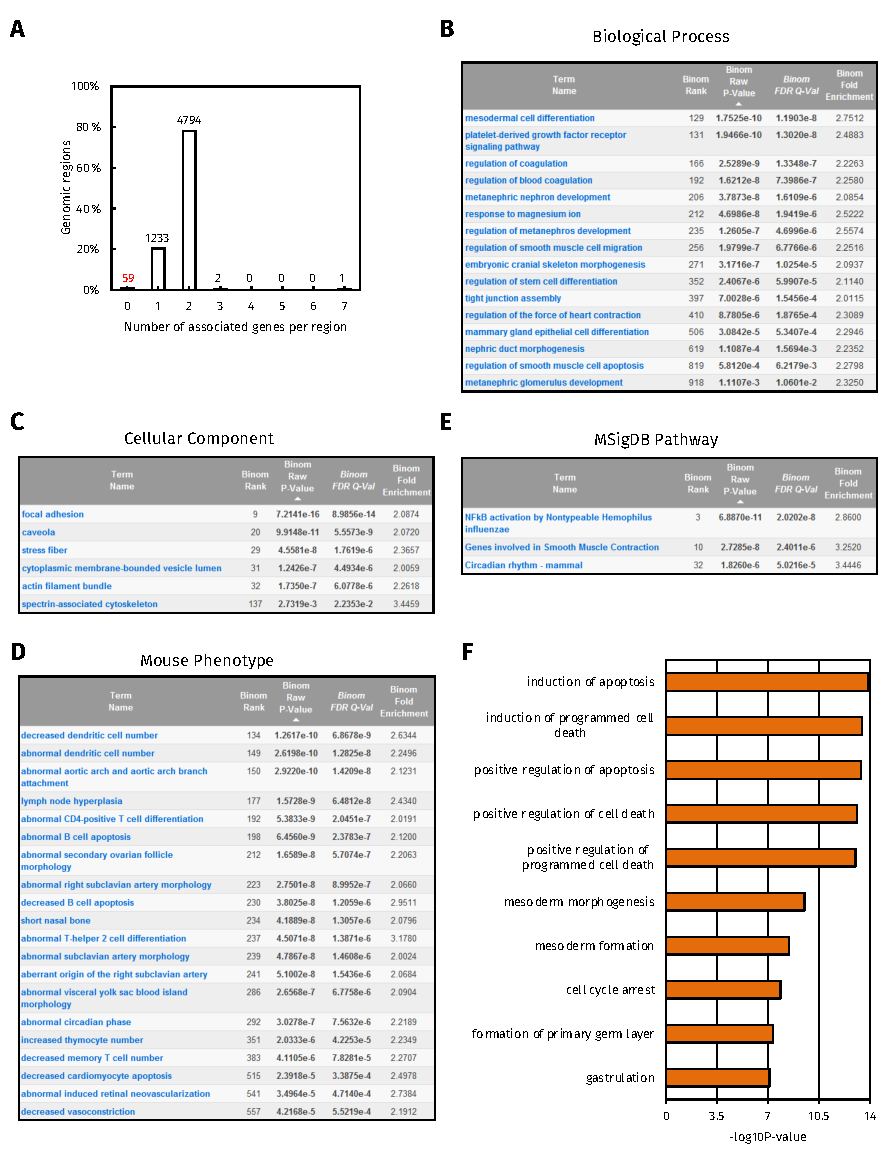
\includegraphics[width=0.9\textwidth]{chapter3/figures_foxo3/fig41.pdf}
    \caption[Gene ontology analysis of FOXO3 peaks by GREAT]{\textbf{Gene ontology analysis of FOXO3 peaks by GREAT. (A)} Histogram showing number of associated genes per peak. (\textbf{B, C, D and E}) GREAT analysis of FOXO3 all peaks (6089). All enriched terms of Biological Process \textbf{(B)}, all enriched terms of Cellular Component \textbf{(C)}, top 20 terms of Mouse Phenotype \textbf{(D)}, and all enriched terms of MSigDB Pathway \textbf{(E)}, were shown. The P-value, FDR, and fold enrichment based on a binomial distribution are also given. \textbf{(F)} Top 10 enriched Biological Process terms of GREAT analysis of FOXO3 top 1000 peaks. The enriched terms were sorted by -$log_{10}$P-value.}
    \label{fig:fig41}
\end{figure}

The top termed returned from the enriched Biological Process was mesodermal cell differentiation, and there were also several other differentiation or development-related terms (\textbf{Figure \ref{fig:fig41}B}). Only recently, FOXO1 and FOXO3 have been identified as essential regulators of the stem cell fate decision in both mouse and human (\cite{renault2009foxo3,zhang2011foxo1}). Our genome-wide analysis of FOXO3 is corroborative to this discovery, which reinforces the discovery that FOXO3 plays a very important role in cell differentiation and development. Interestingly, some other novel functions of FOXO3 were also uncovered, which suggested that FOXO3 regulates the processes involved in coagulation and muscle cell functions (\textbf{Figure \ref{fig:fig41}B}).

The enriched Cellular Component terms were related to adhesion, actin or cytoskeleton (\textbf{Figure \ref{fig:fig41}C}), indicating the FOXO3 target genes are important for providing the mechanical support for cells.

Many enriched Mouse Phenotype terms were related to the apoptosis or differentiation of B and T lymphocytes functions (\textbf{Figure \ref{fig:fig41}D}), indicating that FOXO3 is critical for the immune system by regulating lymphocytes development. Recent studies have shown that FOXO1 is one of the key players in the regulatory network that controls both B and T lymphocytes' functions (\cite{kerdiles2010foxo,lin2010a,ochiai2012a}). Our FOXO3 genomic data strongly suggests that FOXO3 is also involved in the immune system functions, and is likely to function as a redundant factor of FOXO1. Although no direct evidence has demonstrated that FOXO3 controls lymphocyte functions so far, one recent study showed that in the absence of Foxo3, the developmental defects of T regulatory cells caused by the loss of Foxo1 were exacerbated (\cite{kerdiles2010foxo}). Interestingly, the Forkhead transcription factor FOXP3 has long been shown as a key player in T regulatory cells development (\cite{hori2003control}), indicating that FOXOs and FOXPs might form a \enquote{Forkhead code} to regulate lymphocytes' function and development.

The enriched terms returned from MSigDB Pathway indicated that FOXO3 controls the smooth muscle contraction, the activation of the transcription factor NF-$\kappa$B, and the circadian rhythm (\textbf{Figure \ref{fig:fig41}E}), which are consistent with the enriched terms of Biological Process and previous research (\cite{li2012forkhead,zheng2007foxo}).

Having explored the biological functions of the FOXO3 binding events, we did notice that some known functions of FOXO3, like inducing cell cycle arrest and promoting apoptosis, were not unravelled by the gene ontology analysis. However, when the FOXO3 top 1000 peaks (ranked by FDR and fold enrichment from MACS) were put into GREAT to perform the analysis, both cell cycle arrest- and apoptosis-related terms were found significantly enriched in Biological Process (\textbf{Figure \ref{fig:fig41}F}). Indeed, within the top ten most enriched terms, seven of them were about cell cycle arrest and apoptosis, which is consistent with the known functions of FOXO3. GREAT returned 79 enriched terms of Biological Process for the FOXO3 top 1000 peaks, which is much more than the number of enriched terms for the FOXO3 all peaks. Interestingly, the differentiation- and development-related terms were also enriched in the FOXO3 top 1000 peaks (\textbf{Supplementary Table 2}), though not as significant as terms about the cell cycle arrest and the apoptosis.

In summary, the gene ontology analysis recovered many known functions of FOXO3, such as process involved in cell differentiation and development, cell cycle, and apoptosis. The cell cycle arrest- and apoptosis-related genes seem more enriched within the FOXO3 peaks with high binding signals (top 1000). In addition, novel functions of FOXO3 which are related to coagulation and muscle cell contraction were also indicated by the analysis, and further experiments need to be performed to validate the reliability of the new discoveries.

\subsection{Characterisations of the specific and the shared binding events of FOXO3 and FOXK2}

Having confirmed the biological functions of FOXO3, we next focused the analysis on the binding specificities of FOXO3 and FOXK2.

To find out the shared and specific binding events for FOXO3 and FOXK2, their ChIP-seq derived peaks were compared. The number of binding sites between FOXK2 and FOXO3 was quite different. FOXK2 held \textasciitilde 5 times as many binding sites as FOXO3 (\textbf{Figure \ref{fig:fig42}A}). According to the RNA-seq data from The Human Protein Atlas (\cite{uhlen2010towards}), FOXK2 was significantly more abundant (\textasciitilde 30 fold) than FOXO3 in U2OS cells according to their mRNA levels (\textbf{Figure \ref{fig:fig42}B}). Therefore, it is possible that the protein level of FOXK2 is higher than FOXO3 as well. Since factor abundance is important in ChIP-seq experiments, it is tempting to consider the difference of number of binding events as a result of different factor abundance.

\begin{figure}[!h]
    \centering
    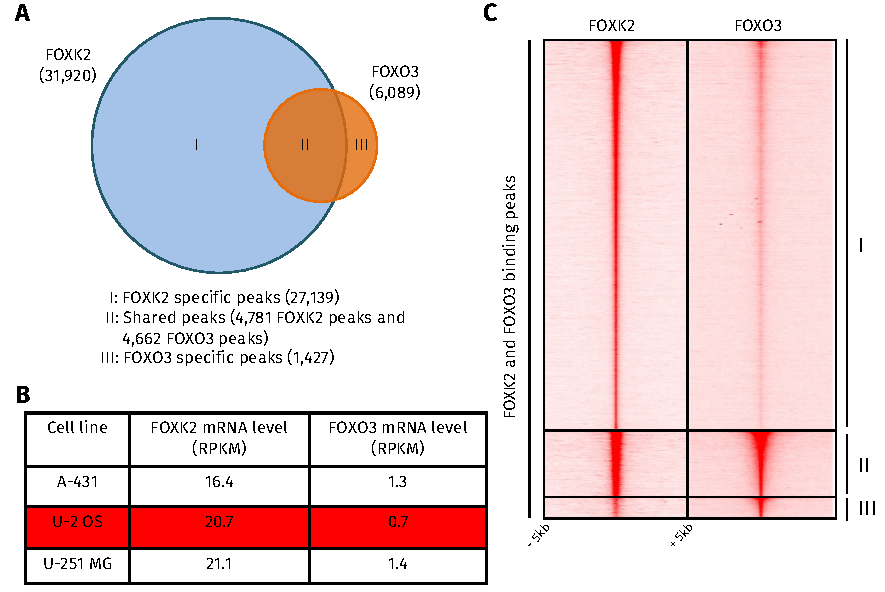
\includegraphics[width=0.9\textwidth]{chapter3/figures_foxo3/fig42.pdf}
    \caption[The overlap of FOXK2 and FOXO3 binding peaks]{\textbf{The overlap of FOXK2 and FOXO3 binding peaks. (A)} Venn diagram showing the overlap of the peaks for FOXO3 and FOXK2. The number of total peaks for each factor and the numbers of FOXK2-specific peaks (I), shared peaks (II) and FOXO3-specific peaks (III) are shown. \textbf{(B)} Quantification of the mRNA levels of FOXK2 and FOXO3 in the indicated cell line. Data was from the RNA-seq experiment in The Human Protein Atlas project (\cite{uhlen2010towards}). Expression values (RPKM, \underline{R}eads \underline{P}er \underline{K}ilobase of exon model per \underline{M}illion mapped reads) from U2OS cells are highlighted. \textbf{(C)} Heatmap of tag density profiles of FOXK2 and FOXO3 around the peaks from the class I, II and III shown in \textbf{(A)}. Peaks in I and II were aligned by the FOXK2 summits, and peaks in III were aligned by the FOXO3 summits. Tags were calculated in every 50 bp bin, and the density profiles were normalised to tags per 10 million total reads per bin. The middle point of each panel (indicated by small arrows below) represents the summit of the peak. 5 kb upstream and 5 kb downstream around the summit were plotted.}
    \label{fig:fig42}
\end{figure}

Since FOXO3 and FOXK2 belong to the same transcription factor family, both shared and specific binding was expected, like members within ETS transcription factor family (\cite{hollenhorst2001mechanisms,wei2010genome-wide}). Here, we define the shared peak as one where peaks overlap by at least one base pair. Indeed, the majority of FOXO3 peaks (~78\%) overlap with FOXK2, and only a small proportion of FOXO3 peaks were specific (\textbf{Figure \ref{fig:fig42}A}). When looking at the sequencing tags around the summit of the specific and shared peaks, there were some FOXO3 binding signals around the summits of FOXK2-specific peaks and vice versa (\textbf{Figure \ref{fig:fig42}C}), but those signals were probably below the threshold used by the MACS or HOMER peak caller. Intriguingly, when the average binding signals of FOXK2 and FOXO3 were compared around the specific and the shared peaks, both factors behaved in a similar way: both of them possessed higher binding signals around the shared peaks than their own specific peaks (\textbf{Figure \ref{fig:fig43}A}). This effect was more prominent in the FOXK2 case (\textbf{Figure \ref{fig:fig43}A}, left panel). The difference of binding signals between the shared and the specific peaks suggests that when binding to the shared regions, both FOXK2 and FOXO3 tend to have higher occupancy. On the other hand, the higher signal intensities within the redundant binding sites could be simply because they are located within open chromatin regions.

\begin{figure}[!h]
    \centering
    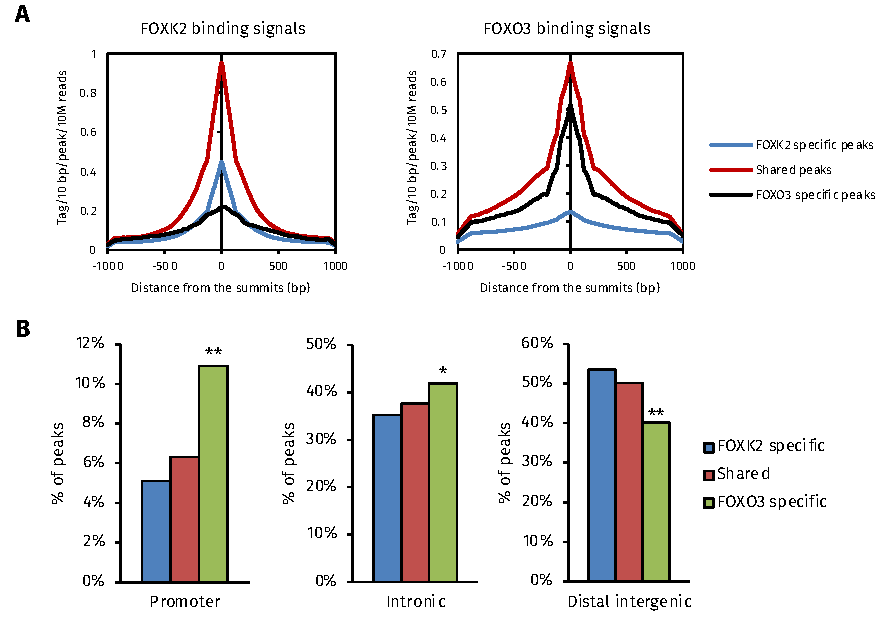
\includegraphics[width=0.9\textwidth]{chapter3/figures_foxo3/fig43.pdf}
    \caption[Tag intensities and genomic distributions of the specific and the shared binding peaks of FOXK2 and FOXO3]{\textbf{Tag intensities and genomic distributions of the specific and the shared binding peaks of FOXK2 and FOXO3. (A)} Quantification of average of tags of FOXK2 (left) and FOXO3 (right) around the summit of indicated peaks. Peaks were aligned by their summits, and a region of -1 and +1 kb relative to the summit was selected. Tags were calculated in every 10 bp bin and normalised to tags per 10 million total reads per bin per peak. \textbf{(B)} Genomic distributions of the indicated peaks. The promoter was defined as 5'-UTR and up to 1 kb upstream from a transcription start site. The distal intergenic region was defined as at least 3 kb upstream from a TSS or at least 3 kb downstream from a TTS. * and ** represent $P<0.005$ and $P<0.0001$, respectively, chi-square test.}
    \label{fig:fig43}
\end{figure}

To further characterise the features of the specific and the shared peaks of FOXK2 and FOXO3, CEAS analysis was performed to check the genomic distribution of the peaks of these three categories. The distributions of the FOXK2-specific peaks and the shared peaks were generally similar, but the FOXO3-specific peaks were more frequently observed within the promoter and the intronic regions and less frequently in the distal intergenic regions (\textbf{Figure \ref{fig:fig43}B}). This indicates that FOXO3, when binding alone, has a different preference towards the promoter and the intronic regions comparing to FOXK2.

Enriched motifs within the peaks often reflect DNA sequence bound by the investigated factor or its interaction partners, and the protein-protein interaction partners often help the factor gain its binding specificity relative to other family members. For example, in budding yeast, Mcm1p interacts with Fkh2p, which helps Fkh2p obtain its specific binding relative to Fkh1p (\cite{hollenhorst2001mechanisms}). Therefore, to further investigate how FOXK2 and FOXO3 obtain their redundant and specific binding sites, \textit{de novo} motif discovery was carried out using HOMER within the 200 bp region centred on the summits of FOXK2 and FOXO3 peaks respectively. The top motifs returned from either FOXK2 or FOXO3 peaks are both Forkhead-like responsive elements, containing the core consensus GTAAACA (\textbf{Figure \ref{fig:fig44}A}). Interestingly, the Forkhead-like responsive elements discovered from FOXK2 and FOXO3 peaks were slightly different: there were some variations not only within the nucleotides in the core consensus and but also in those that are flanking the core consensus (\textbf{Figure \ref{fig:fig44}B}). Generally, the core consensus GTAAACA was the most frequent motif in both FOXK2 and FOXO3 peaks, but A, C, and T at the positions +1, +3, and +6 respectively within the core sequence occurred more frequently in the FOXK2 peaks (\textbf{Figure \ref{fig:fig44}B}). At the flanking regions, there was an overrepresented A or T at the -1 position in both FOXK2 and FOXO3 peaks (\textbf{Figure \ref{fig:fig44}B}), but a G or C was more frequent at the +9 position only in the FOXK2 cistrome (\textbf{Figure \ref{fig:fig44}B}).

\begin{figure}[!h]
    \centering
    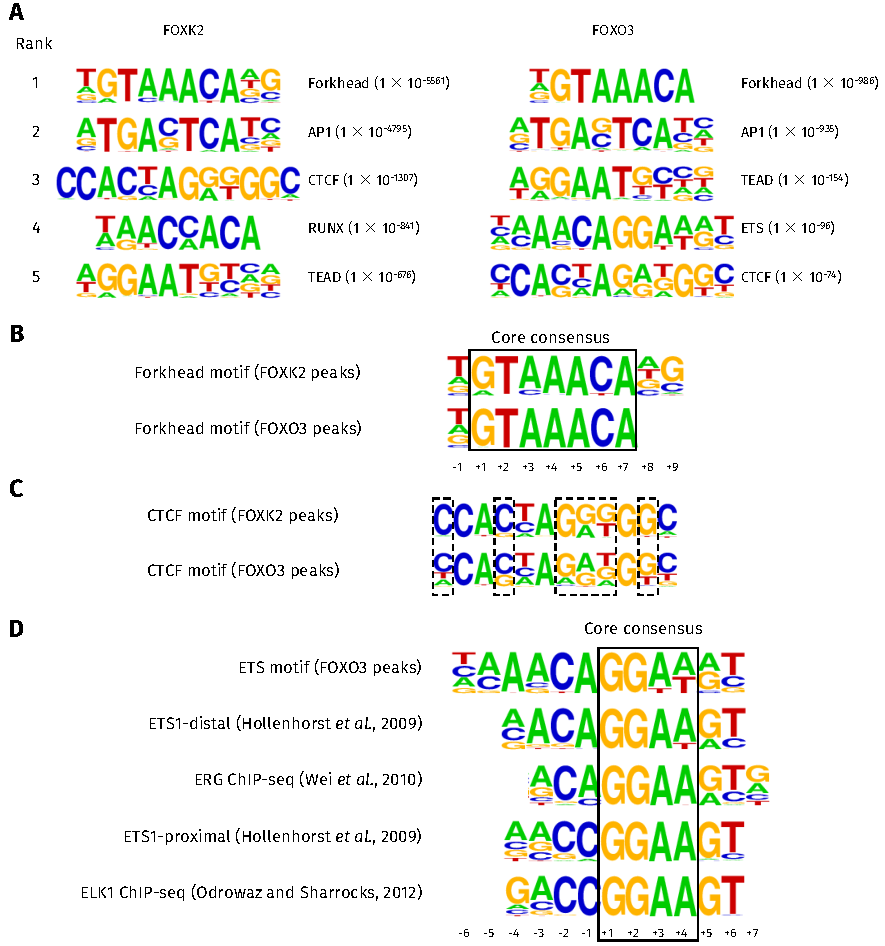
\includegraphics[width=0.9\textwidth]{chapter3/figures_foxo3/fig44.pdf}
    \caption[Overrepresented DNA motifs from FOXK2 and FOXO3 binding peaks]{\textbf{Overrepresented DNA motifs from FOXK2 and FOXO3 binding peaks. (A)} The enriched DNA motifs from FOXK2 and FOXO3 peaks respectively. Motifs are ranked by their P-values which are indicated in parentheses. \textbf{(B)} The comparison of Forkhead motifs returned from the FOXK2 peaks and the FOXO3 peaks. Motifs were aligned to the 5' end of the GTAAACA core sequence, which is highlighted by the rectangle. \textbf{(C)} The comparison of the CTCF motifs returned from the FOXK2 peaks and the FOXO3 peaks. Dotted rectangle highlights the positions which hold higher information content in the CTCF motif from the FOXK2 peaks. \textbf{(D)} The comparison of the ETS motif from the FOXO3 peaks with motifs from ETS1, ERG and ELK1 ChIP-seq. Motifs were aligned to the 5' of the GGAA core sequence which is highlighted by the rectangle.}
    \label{fig:fig44}
\end{figure}

In addition to the Forkhead-like responsive elements, the AP1 motif, the CTCF motif, and the TEAD motif were also found overrepresented within both FOXK2 and FOXO3 peaks, but the RUNX motif and the ETS motifs were only enriched in FOXK2 and FOXO3 peaks respectively (\textbf{Figure \ref{fig:fig44}A}). The AP1 motif and the TEAD motif from the FOXK2 peaks are essentially the same as those from the FOXO3 peaks, but the CTCF motif enriched in the FOXK2 peaks possessed higher information content (stronger motif) than that enriched in the FOXO3 peaks (\textbf{Figure \ref{fig:fig44}C}), suggesting that the CTCF motif might be more overrepresented within the FOXK2 cistrome. The ETS motif from FOXO3 peaks resembled the motifs enriched within the ETS1 distal binding peaks (\textbf{Figure \ref{fig:fig44}D}), but differed from motifs enriched within ETS proximal binding peaks, the ERG binding regions or the ELK1 cistrome (\textbf{Figure \ref{fig:fig44}D}), indicating that FOXO3 might cooperate with specific ETS factors to regulate transcription.

In summary, the numbers of binding sites of FOXK2 and FOXO3 are quite different. FOXK2 has about \textasciitilde 5 times as many binding sites as FOXO3 does. These two factors possess both shared and specific binding regions, and the majority (\textasciitilde 78\%) of FOXO3 binding events are also bound by FOXK2. Such a great extent of overlap between the binding sites of these two proteins is quite unexpected, because previous studies do not suggest any functional redundancy between FOXK2 and FOXO3 (\cite{brunet1999akt,marais2010cell,ji2012the}). The FOXO3 specific binding events are more enriched in the promoter and intronic regions, but occur less frequently within distal intergenic regions. Forkhead-like motifs containing the core sequence GTAAACA are enriched within both FOXK2 and FOXO3 binding event, though there are some sequence variances between the two Forkhead-like motifs. Other transcription factor binding motifs are also enriched within the FOXK2 and the FOXO3 cistromes, indicating the interactions with other transcription factors might help them gain their specific binding events.

\subsection{Nucleotides flanking the Forkhead core consensus are important for the FOXK2 DNA binding both \textit{in vivo} and \textit{in vitro}}

\begin{figure}[!ht]
    \centering
    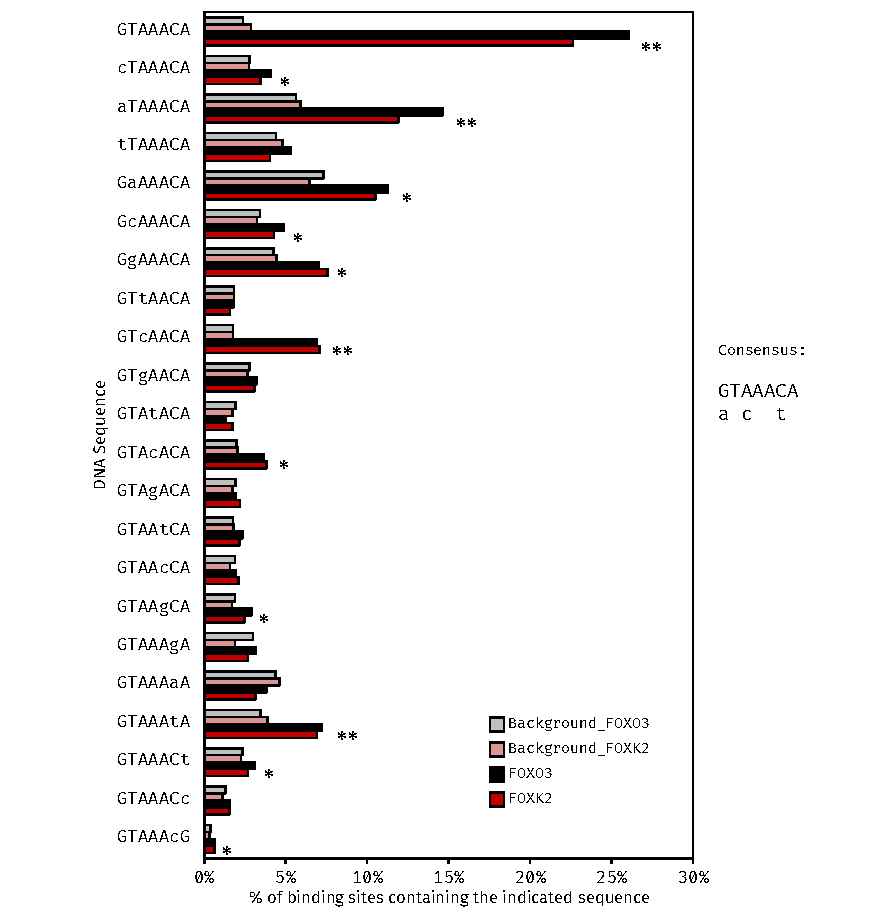
\includegraphics[width=0.9\textwidth]{chapter3/figures_foxo3/fig45.pdf}
    \caption[Binding specificities of FOXK2 and FOXO3 within the Forkhead core consensus]{\textbf{Binding specificities of FOXK2 and FOXO3 within the Forkhead core consensus.} The occurrence of each indicated heptameric sequences within the 200 bp regions centred on the FOXK2 or FOXO3 summit. * represents $P<0.0001$ by a chi-square test. ** represents $P<0.0001$ and indicates the sequences that have 2-fold enrichment of occurrence over the background. The background sequences were randomly chosen from the genome based on the genomic distribution of FOXK2 and FOXO3 binding peaks respectively. The summarised consensus is shown at the right.}
    \label{fig:fig45}
\end{figure}

Given the similarity and the difference of the motifs enriched within FOXK2 and FOXO3 peaks, it is reasonable to speculate that FOXK2 and FOXO3 have a related but different specificity towards the Forkhead consensus, and their interactions with different transcription factors might also contribute to their redundant and specific binding. To test these hypotheses, we first investigated whether FOXK2 and FOXO3 have different specificities to the nucleotides within and flanking the Forkhead core consensus. To this end, we checked the occurrences of a series of heptameric sequences within the 200 bp regions centred on the summit of FOXK2 or FOXO3 bound regions based on the core GTAAACA sequence with each containing a single nucleotide substitution. Random sets of sequences with the same length and similar genomic distribution were chosen as background sequences for parallel comparison. The most frequent and enriched sequences in both cases were the consensus core GTAAACA, but many other sequences were also overrepresented compared to the background sequence (indicated by * in \textbf{Figure \ref{fig:45}}). If setting a threshold of 2-fold over the background, the enriched sequences contained GTAAACA, ATAAACA, GTCAACA, and GTAAATA, which could be summarised as RTMAAYA. This is extremely similar with the sequence of the previous results from in vitro selection of binding sites of seven Forkhead proteins (\cite{pierrou1994cloning}). More importantly, the frequency of each heptameric was nearly identical within FOXK2 peaks and FOXO3 peaks (\textbf{Figure \ref{fig:fig45}}). In addition, the occurrences of GTAAACA, ATAAACA, GTCAACA and GTAAATA were also very similar among the FOXK2-specific peaks, the shared peaks, and the FOXO3-specific peaks (data not shown). These findings indicate that FOXK2 and FOXO3 have very similar binding specificities towards the sequences within the Forkhead core consensus.

Having checked the preferences of FOXK2 and FOXO3 within the Forkhead core sequence, we next investigated whether the DNA sequence flanking the core would influence FOXK2 or FOXO3 binding. To gain an insight into the binding specificities of FOXK2 and FOXO3 at the flanking regions, 5 base pairs upstream and downstream of the GTAAACA core sequence were extracted from the ChIP-seq binding regions, and the frequencies of A, C, G and T nucleotide were counted at each flanking position (\textbf{Figure \ref{fig:fig46}A}). As a comparison, 5 base pairs upstream and downstream of the GTAAACA sequence from the whole genome were also extracted as background.

\begin{figure}[!h]
    \centering
    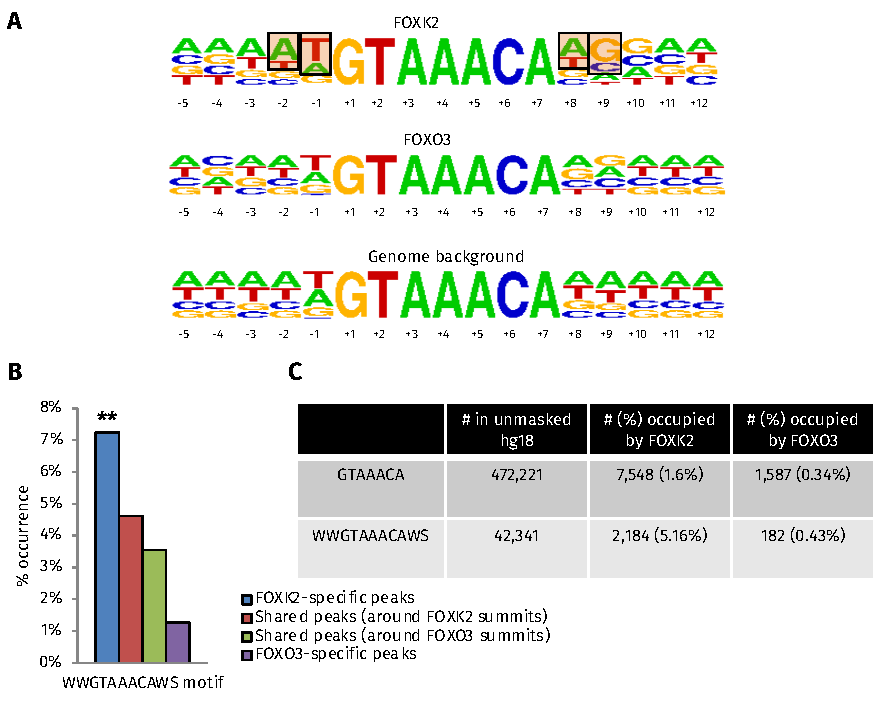
\includegraphics[width=0.9\textwidth]{chapter3/figures_foxo3/fig46.pdf}
    \caption[Nucleotides flanking the core sequence better discriminate FOXK2 from FOXO3 binding]{\textbf{Nucleotides flanking the core sequence better discriminate FOXK2 from FOXO3 binding. (A)} The occurrence of sequences at the flanking regions of the GTAAACA core sequence. 5 bp upstream and 5 bp downstream the core were investigated. Motifs were drawn according to the nucleotide frequency at each position. Yellow rectangles indicate nucleotides whose frequencies are higher than a random distribution using the genome as a background. \textbf{(B)} Percentage of indicated peaks ($\pm$ 200 bp from the summit) that contain the motif WWGTAAACAWS. ** represents $P<0.0001$, chi-square test. \textbf{(C)} Statistics of the sequences GTAAACA and WWGTAAACAWS in the human genome (unmasked hg18). The numbers of the sequences and the percentage occupied by FOXK2 and FOXO3 are shown.}
    \label{fig:fig46}
\end{figure}

In both cases, there was no strong preference within the flanking regions, but the frequency of some nucleotides at certain positions near the core of FOXK2 was indeed much higher than the genome background (\textbf{Figure \ref{fig:fig46}A}, yellow rectangles). FOXK2 preferred an A/T and T/A at the positions -2 and -1, an A/T and G/C at the positions +8 and +9 positions respectively (\textbf{Figure \ref{fig:fig46}A}, top panel). The frequency of nucleotide occurrence flanking the core was similar to background in the FOXO3 case (\textbf{Figure \ref{fig:fig46}A}, middle panel). These observations indicate that nucleotides flanking the core sequence might partially dictate the binding specificity of FOXK2, but their contribution to FOXO3 specific binding, if any, are marginal. The most frequent FOXK2 binding motif including the nucleotides flanking the core can be summarised as an extended motif: WWGTAAACAWS, which is very similar to the original motif returned from HOMER \textit{de novo} discovery. Indeed, this extended motif was significantly more enriched within FOXK2 specific binding peaks compared to either the shared or the FOXO3-specific peaks (\textbf{Figure \ref{fig:fig46}B}). When looking on a genome-wide scale, only 1.6\% of total GTAAACA in the human genome was occupied by FOXK2, but 5.16\% of total WWGTAAACAWS was bound by FOXK2 (\textbf{Figure \ref{fig:fig46}C}). In contrast, 0.34\% of total GTAAACA in the whole genome was occupied by FOXO3, and the percentage (0.43\%) of WWGTAAACAWS bound by FOXO3 was only slightly higher than that of the core GTAAACA motif (\textbf{Figure \ref{fig:fig46}C}). This implies that FOXK2, but not FOXO3, possesses some sequence preference at the regions flanking the Forkhead core consensus.

The sequence analysis within the FOXK2 and FOXO3 binding sites suggest that nucleotides flanking the Forkhead core consensus play some role in the DNA binding of FOXK2. However, \textit{in vivo} binding does not necessarily reflect the intrinsic specificity of a factor due to the presence of many other DNA binding factors in the nucleus. To test whether the sequences in the flanking regions of the Forkhead consensus affect the intrinsic affinity of FOXK2 to DNA, \textit{in vitro} competition EMSAs were performed. The DNA sequence from the \textit{MMP9} locus where FOXK2 binds was used as a binding site. The wild type binding site contains the sequence TT\underline{GTAAACA}AG (\textbf{Figure \ref{fig:fig47}A}). The mutant binding sites also contain the Forkhead core consensus GTAAACA, but the nucleotides at either 5' or 3' to the core consensus were mutated (\textbf{Figure \ref{fig:fig47}A}). We tested the abilities of these unlabelled sequences to compete with the \sus{32}P-labelled wild-type sequence. Reduced binding between FOXK2 and the \sus{32}P-labelled wild-type sequence was observed with the addition of increasing concentrations of both the wild-type and the mutant unlabelled sequences (\textbf{Figure \ref{fig:fig47}B}, lanes 3-14), indicating FOXK2 can bind to both the wild-type and the mutant sequences. However, neither of the mutant probes was as efficient as the wild- type probe to compete for the binding of FOXK2 (\textbf{Figure \ref{fig:fig47}B}, compare lanes 3, 7 and 11). This suggests that nucleotides flanking the Forkhead core consensus indeed affect the intrinsic FOXK2 DNA binding, although the difference between the WT sequence and the Mut2 sequence failed to reach statistical significance when relatively low concentrations of unlabelled sequences were added (\textbf{Figure \ref{fig:fig47}C}). Mutations of nucleotides at the 5' flank of the core consensus had greater effect than the mutations at the 3' flank of the core consensus (\textbf{Figure \ref{fig:fig47}B}, compare lanes 9 and 13), indicating sequences at the 5' flank of the core consensus contribute relatively more to the FOXK2 DNA binding.

Interestingly, the competition EMSA results were consistent with the crystal structure of the DNA-binding domain of FOXK2 with DNA (\cite{tsai2006crystal}). The DNA sequence used in the structure of FOXK2 DBD-DNA complex was 5'-TGTT\underline{GTAAA}- \underline{CA}ATACA-3'. Base-specific contacts were observed not only within the GTAAACA core consensus, but also at the TpT dinucleotides upstream the consensus and ApT dinucleotides downstream the consensus, indicating the specific interactions between FOXK2 and the DNA exist at the flanking regions (\cite{tsai2006crystal}). In addition, such specific interactions were not seen in the structures of FOXO3 DBD or FOXA3 DBD with DNA (\cite{tsai2006crystal,clark1993co-crystal}).

\begin{figure}[!h]
    \centering
    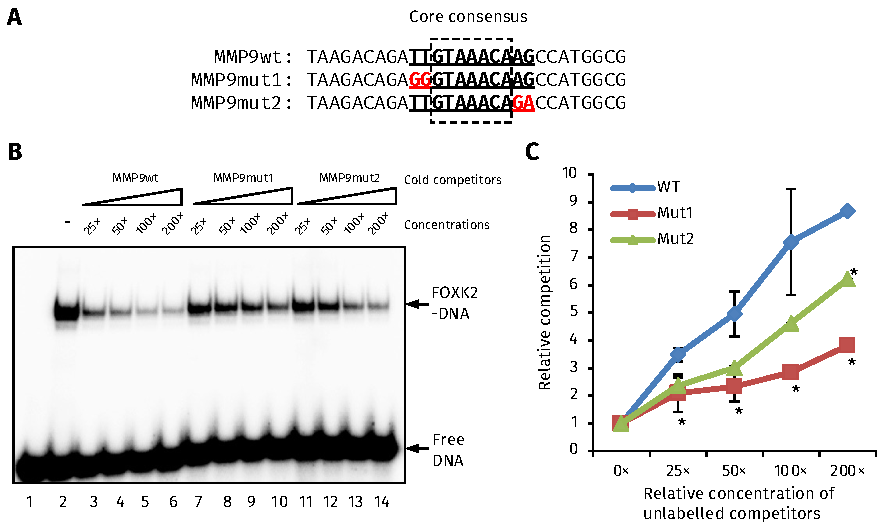
\includegraphics[width=0.9\textwidth]{chapter3/figures_foxo3/fig47.pdf}
    \caption[Competition EMSA experiments to assess the effect of the nucleotides flanking the Forkhead consensus on FOXK2 DNA binding]{\textbf{Competition EMSA experiments to assess the effect of the nucleotides flanking the Forkhead consensus on FOXK2 DNA binding. (A)} DNA sequences used in the experiments. The Forkhead core consensus from the FOXK2 binding region in the \textit{MMP9} regulatory region is highlighted, and the mutations are shown in red colours. \textbf{(B)} Competition EMSA experiments to test the contribution of the nucleotides flanking the Forkhead consensus to the intrinsic binding affinity of FOXK2. Experiments were performed using 90 nM of purified FOXK2 DNA-binding domain and the \sus{32}P-labelled wild-type sequence, together with varying concentrations of the indicated unlabelled binding sites. The unlabelled competitors and their concentrations relative to the \sus{32}P-labelled binding site (taken as 1$\times$) are indicated above the gel. No protein was added at the lane 1. No cold competitors were added at the lane 2. \textbf{(C)} Relative quantification of the FOXK2- DNA complex in \textbf{(B)}. The intensity of FOXK2-DNA complex in the absence of competitors was taken as 1. The reciprocals of the intensity of FOXK2-DNA complex were plotted against the relative concentrations of the unlabelled competitors. The error bars represent the standard deviations from two independent experiments. * and ** represent $p<0.05$ and $p<0.01$ respectively.}
    \label{fig:fig47}
\end{figure}

In summary, both FOXK2 and FOXO3 bind to the consensus RTMAAYA, with GTAAACA being the most overrepresented binding sequence in the cistrome of both factors. Generally, FOXK2 and FOXO3 do not have discernible specificities towards the core sequence. However, FOXK2 has some sequence preference at the regions flanking the core sequence, and the extended motif of FOXK2 can be summarised as WWGTAAACAWS. Indeed, nucleotides at the flanking regions are important for the intrinsic DNA binding of FOXK2, since mutations at the nucleotides flanking the Forkhead consensus reduce the DNA binding of FOXK2 \textit{in vitro}. Similar experiments need to be done in future using the FOXO3 DNA-binding domain to investigate whether FOXO3 also has sequence preferences at the flanking regions of the Forkhead core consensus.

\subsection{Different transcription factors might contribute to the specific binding of FOXK2 and FOXO3}

After exploring the specificities of FOXK2 and FOXO3 towards the Forkhead consensus, we next performed a detailed analysis on other motifs identified from the ChIP-seq derived peaks of FOXK2 and FOXO3, and further investigated the potential roles of other transcription factors on FOXK2 and FOXO3 binding specificities.

To this end, we first checked the enrichment of different motifs discovered from the FOXK2 and FOXO3 cistromes (\textbf{Figure \ref{fig:fig44}A}) within the top 1000 peaks (ranked by the FDR and fold enrichment from MACS) from FOXK2-specific, shared, and FOXO3-specific binding regions respectively. Consistent with previous results, the Forkhead core consensus GTAAACA motif was enriched in all shared and specific peaks of FOXK2 and FOXO3, but the extended Forkhead motif WWGTAAACAWS was more enriched in regions where FOXK2 binds (\textbf{Figure \ref{fig:fig48}A}). The enrichment of the AP1 motif was relatively similar across different classes of peaks (\textbf{Figure \ref{fig:fig48}A}). However, the TEAD motif, the RUNX motif and the CTCF motif were more enriched where FOXK2 binds, and the ETS motif was more enriched where there is FOXO3 binding (\textbf{Figure \ref{fig:fig48}A}).

The differential enrichment of motifs within the specific binding sites of FOXK2 and FOXO3 respectively suggest that they can co-bind with various transcription factors. However, the presence of a motif does not predict the binding of a transcription factor. This is especially the case when it comes to the CTCF transcription factors, where there is some dispute on its binding consensus (\cite{cuddapah2009global,martin2011genome-wide,rhee2011comprehensive}). Therefore, to gain an insight into the potential co-binding of FOXO3/FOXK2 and other transcription factors, and more importantly, to investigate whether the co-binding potentially influences their specificities, we looked into multiple ChIP-seq data sets including ETS1 and RUNX1/3 in Jurkat T cells (\cite{hollenhorst2009dna}), and CTCF in K562 cells (\cite{ernst2011mapping}; and ENCODE project), which might contribute to their binding events.

\begin{figure}[!ht]
    \centering
    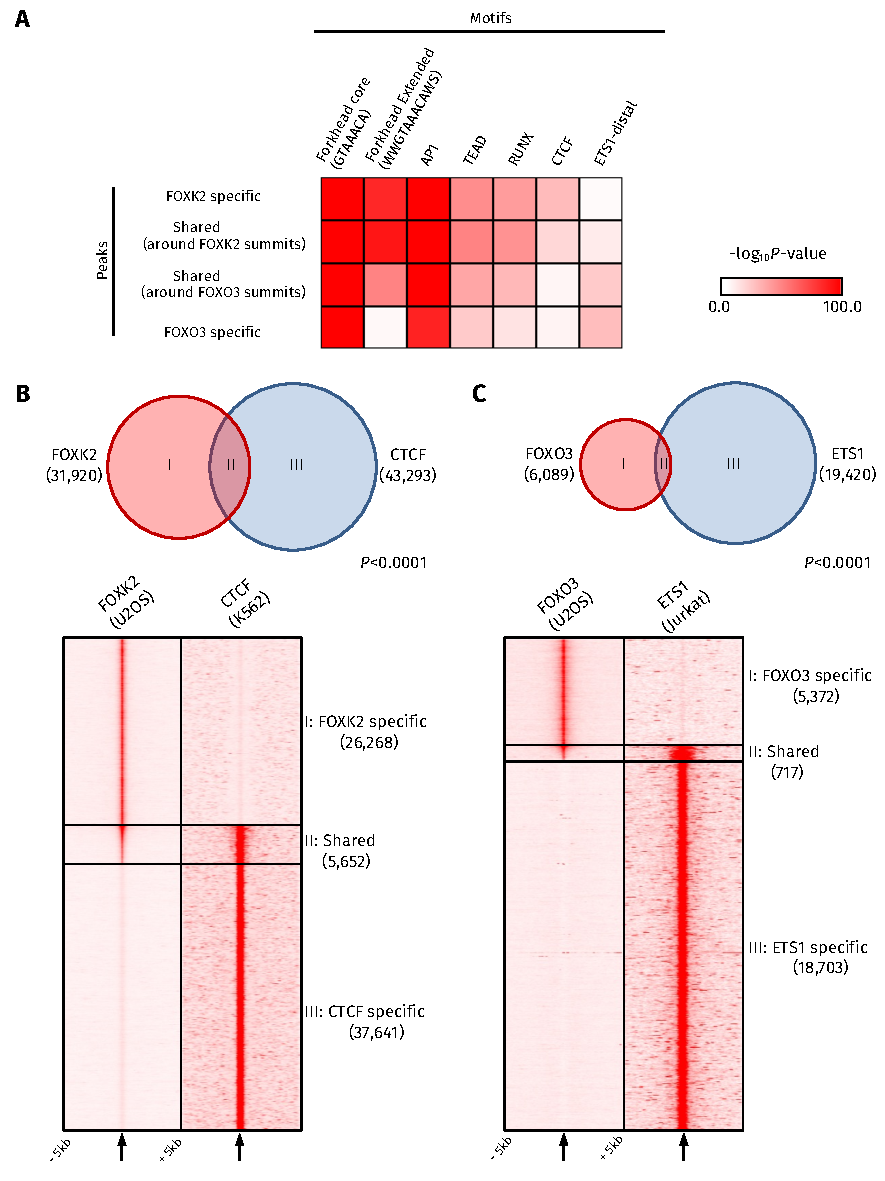
\includegraphics[width=0.9\textwidth]{chapter3/figures_foxo3/fig48.pdf}
    \caption[Co-binding of FOXK2 and FOXO3 with other transcription factors]{\textbf{Co-binding of FOXK2 and FOXO3 with other transcription factors. (A)} The enrichment of each motif within  $\pm$200 bp of the summits from the indicated peaks (top 1000 peaks, ranked by the FDR and fold enrichment). The heatmap was generated using the -$log_{10}$P-value of the indicated motifs calculated by a hypergeometric distribution. \textbf{(B) Top,} a Venn diagram showing the overlap between the FOXK2 peaks and the CTCF peaks. Numbers of total FOXK2 peaks and CTCF peaks were indicated. I, II, and III represent FOXK2-specific peaks, shared peaks and the CTCF-specific peaks respectively. The P-value of the overlap was calculated by a chi-square test. \textbf{Bottom,} heatmap of tag density profiles of FOXK2 and CTCF around the three classes of peaks shown at the top. Numbers of peaks within each class are indicated. Tags were calculated in every 50 bp bin, and the density profiles were normalised to tags per 10 million total reads per bin. The middle point of each panel (indicated by small arrows below) represents the summit of the FOXK2 or CTCF peak. 5 kb upstream and 5 kb downstream around the summit were plotted. Peaks in class I and II were aligned by the FOXK2 summits, and peaks in class III were aligned by the CTCF summits. \textbf{(C)} The same analysis as \textbf{(B)} with the FOXO3 and ETS1 ChIP-seq data.}
    \label{fig:fig48}
\end{figure}

The overlap between RUNX1/3 with FOXK2 and FOXO3 was only marginal (data not shown), indicating that they do not tend to bind to the same locations. The cell type difference might be a reason, and it is also possible that FOXK2 co-localises with a different RUNX factor like RUNX2. Significant overlaps between FOXK2 and CTCF, and between FOXO3 and ETS1 were observed (\textbf{Figure \ref{fig:fig48}B} and \textbf{(C)}). Consistent with the motif enrichment analysis, the overlap between FOXK2 and CTCF was more significant than the overlap between FOXO3 and CTCF ($P<0.0001$, chi-square test), and the overlap between FOXO3 and ETS1 was more significant than that between FOXK2 and ETS1 ($P<0.0001$, chi-square test). Furthermore, detailed analysis on tag density profiles on the overlapping peaks of these factors demonstrated that the reads of CTCF and ETS1 were nicely clustered around the summit of FOXK2 and FOXO3 respectively, indicating that CTCF and ETS1, indeed, bind to the same locations or in close proximity to FOXK2 and FOXO3 respectively (\textbf{Figure \ref{fig:fig48}B} and \textbf{(C)}, class II peaks). These findings indicate that CTCF and ETS1 might contribute to FOXK2 and FOXO3 specific binding as well as their biological functions respectively.

In summary, the possibilities that other transcription factors contribute to the specific binding events of FOXK2 and FOXO3 have been explored through bioinformatic analyses. The CTCF motif was more enriched within the FOXK2 cistrome, while the ETS1 motif was more enriched within the FOXO3 cistrome. Co-localisation of binding events between FOXK2 and CTCF, and between FOXO3 and ETS1 were observed, indicating that potential interactions with other transcription factors might partially contribute to FOXK2 and FOXO3 binding specificity and/or help specify their transcriptional regulatory activities.

\subsection{The enigmatic relationship between FOXK2 and FOXO3 binding}

Having characterised the specific and the shared binding events of FOXK2 and FOXO3, we next investigated the relationship of the DNA binding between these two factors.

Since FOXO3 and FOXK2 belong to the same family and possess many shared binding events, one would expect that they compete for binding sites within those shared peaks, which happens when different factors bind to the same sites (\cite{pierce2003sum1,zhou2011integrated}). On the other hand, the fact that binding signals of both FOXK2 and FOXO3 are generally higher around the shared peaks indicates that an assisted binding mechanism is also possible. Indeed, Forkhead transcription factors, like FOXA1, have been demonstrated as pioneer priming factors for several nuclear receptors like ER (\cite{hurtado2011foxa1}) and AR (\cite{wang2011reprogramming}), though the role of FOXA1 in the latter case is more complicated. FOXK2 is constantly nuclear (\cite{marais2010cell}), but FOXO3 is sequestered in the cytoplasm under normal condition and goes into the nucleus when the PI3K/AKT signalling is inhibited. This resembles the behaviour of those nuclear receptors which also translocate to the nucleus upon receiving a signal through ligand binding. Therefore, it is also tempting to speculate that FOXK2, which is constantly nuclear, acts as a pioneer priming factor for FOXO3 in U2OS cells.

\begin{figure}[!ht]
    \centering
    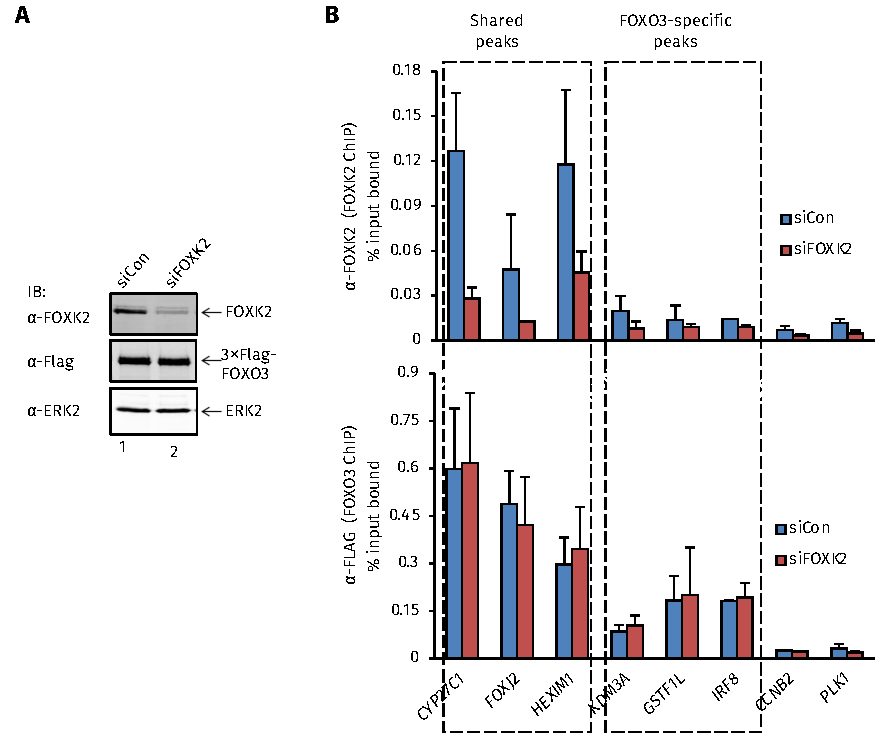
\includegraphics[width=0.9\textwidth]{chapter3/figures_foxo3/fig49.pdf}
    \caption[Knockdown of FOXK2 has little effect on the DNA binding of FOXO3]{\textbf{Knockdown of FOXK2 has little effect on the DNA binding of FOXO3. (A)} Western blot analysis showing the endogenous FOXK2 protein level after the depletion of FOXK2. The U2OS-FOXO3 stable cell line was transfected with a non-targeting siRNA or a siRNA against FOXK2. Protein expression levels were examined by immunoblotting (IB) with the indicated antibodies. \textbf{(B)} The U2OS-FOXO3 stable cell line was treated with doxycycline to induce the expression of the FLAG-tagged FOXO3 transgene, and were transfected with 20 nM non-targeting siRNA or siRNA against FOXK2. LY294002 were added to cells 2 hours before crosslinking the cells. ChIP experiments were performed either using a FOXK2 antibody (top) or a FLAG antibody (bottom). The shared regions and the FOXO3-specific regions are indicated by dashed rectangles. The error bars represent the standard deviations from two independent experiments.}
    \label{fig:fig49}
\end{figure}

To test whether FOXK2 competes with or primes for the FOXO3 binding, 3$\times$FLAG- FOXO3 was induced to the level comparable to the endogenous FOXO3 by adding doxycycline (\textbf{Figure \ref{fig:fig11}B}, lane 3), and FOXO3 was activated by the treatment of cells with LY294002. ChIP experiments were performed after the knockdown of FOXK2 by siRNA transfection, and the DNA binding was measured by locus-specific qPCR. Six peaks from the ChIP-seq data, including three shared peaks and three FOXO3 specific peaks, were tested. The \textit{CCNB2} and the \textit{PLK1} loci were used as negative control regions. Western blot analyses showed that the FOXK2 protein level was significantly reduced after the knockdown of FOXK2, although there was still some detectable FOXK2 protein (\textbf{Figure \ref{fig:fig49}A}). The expression of 3$\times$FLAG-FOXO3 was unaffected by the treatment of the FOXK2 siRNA (\textbf{Figure \ref{fig:fig49}A}). After the depletion of FOXK2, either increased (indicating competition with FOXK2) or decreased (indicating primed by FOXK2) FOXO3 binding was expected. The FOXK2 binding signals were reduced at the shared binding regions after the treatment with siFOXK2, and its binding levels at the FOXO3-specific regions were comparable to the background (\textbf{Figure \ref{fig:fig49}B}, top panel). However, the FOXO3 binding signals were hardly affected by the FOXK2 knockdown (\textbf{Figure \ref{fig:fig49}B}, bottom panel). It seems that under current experimental conditions, neither competitive nor cooperative binding between FOXK2 and FOXO3 could be detected.

To further investigate the relationship between FOXK2 and FOXO3 DNA binding, FOXK2 ChIP experiments were performed after the activation of the endogenous FOXO3 by the treatment of LY294002. Similarly, no discernible changes of FOXK2 binding could be observed on the tested regions (\textbf{Figure \ref{fig:fig50}A}). However, addition of LY294002 will inhibit PI3K/ATK signalling, which might also affect FOXK2 DNA binding. Since previous immunofluorescence experiments demonstrate that some FOXO3 protein is located in the nucleus under normal cell culture condition (\textbf{Figure \ref{fig:fig11}C}), we just forced the overexpression of FOXO3 to increase its nuclear concentration by simply adding a high concentration of doxycycline under normal cell culture condition (with FCS, without LY294002) to circumvent any possible effects of LY294002 on FOXK2 DNA binding. Western blot analyses showed that the expression of 3$\times$FLAG-FOXO3 was significantly elevated after the addition of a high concentration of doxycycline (\textbf{Figure \ref{fig:fig50}B}). More importantly, the overexpression of FOXO3 resulted in an increased DNA binding on all tested regions even without LY294002 treatment (\textbf{Figure \ref{fig:fig50}B}, top panel). However, similar to previous results, the changes of FOXK2 binding were only marginal, even though the binding of FOXO3 was significantly increased at the same region (\textbf{Figure \ref{fig:fig50}B}, bottom panel).

\begin{figure}[!h]
    \centering
    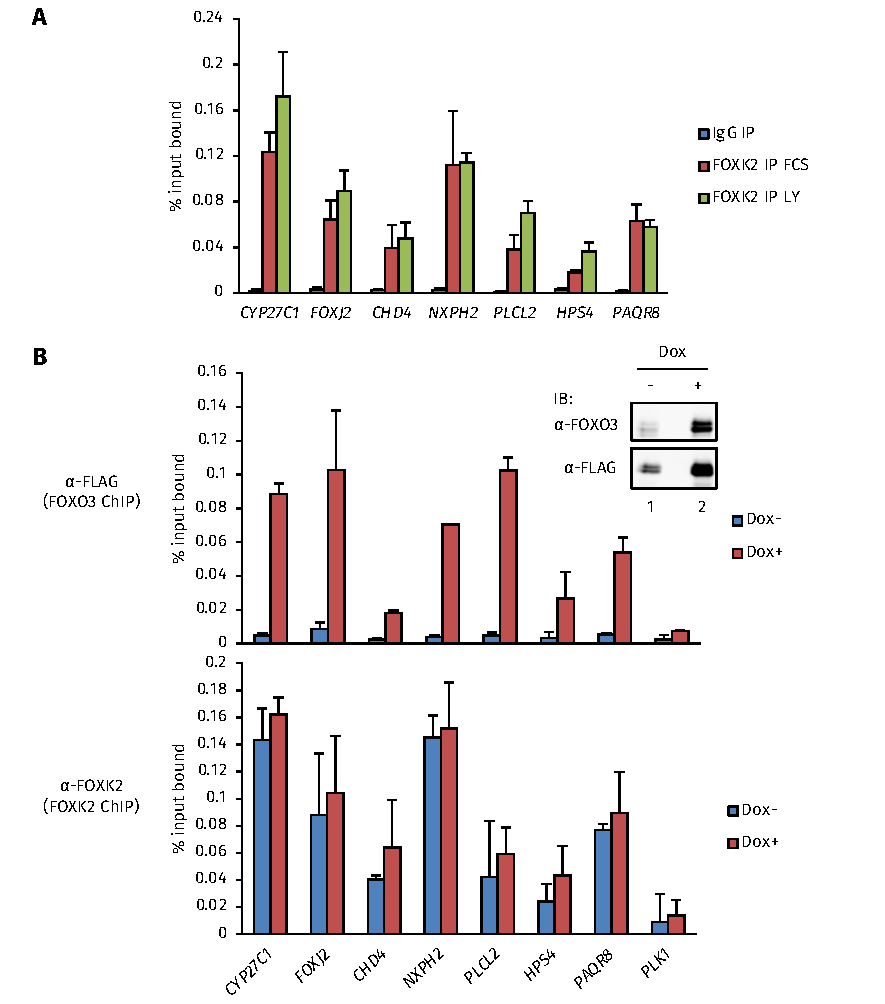
\includegraphics[width=0.9\textwidth]{chapter3/figures_foxo3/fig50.pdf}
    \caption[Changes of FOXO3 binding do not significantly affect FOXK2 binding]{\textbf{Changes of FOXO3 binding do not significantly affect FOXK2 binding. (A)} FOXK2 ChIP experiments with or without the treatment with LY294002. U2OS cells were cultured under normal condition (FCS) or treated with LY294002 (LY) for 2 hours before performing the experiments. ChIP was done using a FOXK2 antibody. A non-specific IgG antibody was also included as a control. The error bar represents the standard deviation from two independent experiments. \textbf{(B)} FOXO3 and FOXK2 ChIP with or without FOXO3 overexpression. The U2OS-FOXO3 stable cell line was either untreated (Dox-) or treated with 1 $\mu$g/mL doxycycline (Dox+) for 24 hours before experiments. ChIP experiments were done using a FLAG antibody (top) or a FOXK2 antibody (bottom). The \textit{PLK1} locus was used as a negative control region. The error bar represents the standard deviation from two independent experiments. Western blot analysis showing the overexpression of the FLAG-tagged FOXO3 transgene after the addition of doxycycline is shown at the top right corner. The U2OS-FOXO3 stable cell line was treated with 1 $\mu$g/mL doxycycline for 24 hours. Protein expression levels were examined by immunoblotting (IB) with the indicated antibodies.}
    \label{fig:fig50}
\end{figure}

The observations that changes of FOXK2 binding does not affect the FOXO3 binding and vice versa suggest that their DNA binding events are independent of each other. It is likely that FOXK2 and FOXO3 bind to the same site but in different cells. If this is the case, changes of the binding of one factor will only affect the binding of the other factor in a subfraction of the cells, which might not be able to be detected by our ChIP experiments. It is also possible that FOXK2 and FOXO3 bind to the same region but at different sites, which cannot be discriminated by the resolution of sonication-based ChIP-seq method that we use. However, it is also likely that current ChIP experiments which analyse the steady-state \textit{in vivo} protein-DNA interactions are unable to detect the subtle dynamic changes of DNA-binding of FOXK2 and FOXO3.

To gain a preliminary idea of whether FOXK2 and FOXO3 bind to different sites or not, we looked into the redundant peaks and analysed the distance between the summits of FOXK2 and FOXO3. The majority of FOXO3 and FOXK2 summits were within 160 bp, though a small proportion of their summits were relatively far away from each other (\textbf{Figure \ref{fig:fig51}A}). This indicates that the exact binding sites of FOXK2 and FOXO3 are close, if not the same. Since the heptameric sequences GTAAACA, ATAAACA, GTCAACA and GTAAATA (hereafter known as FOXK2/O3 motifs) are the most enriched sequences within the FOXK2 and FOXO3 cistromes (\textbf{Figure \ref{fig:fig45}}), they are presumably the direct binding sequences of FOXK2 and FOXO3. Within the shared peaks, \textasciitilde 58\% of them contain at least one FOXK2/O3 motif. Among these peaks, most only contain one site of FOXK2/O3 motif per peak within the 200-bp region around the FOXK2 summit (\textbf{Figure \ref{fig:fig51}B}). The analysis on the FOXO3 summits within the shared peaks yielded the same result (data not shown). These findings indicate that in most cases, there is only one site available for Forkhead proteins to bind at the shared peaks. Therefore, based on the proximity of their summit and the occurrence of the FOXK2/O3 motifs within the peaks, the favourable extrapolation from these results would be that the binding of FOXK2 and the binding FOXO3 are likely mutually exclusive.

\begin{figure}[!h]
    \centering
    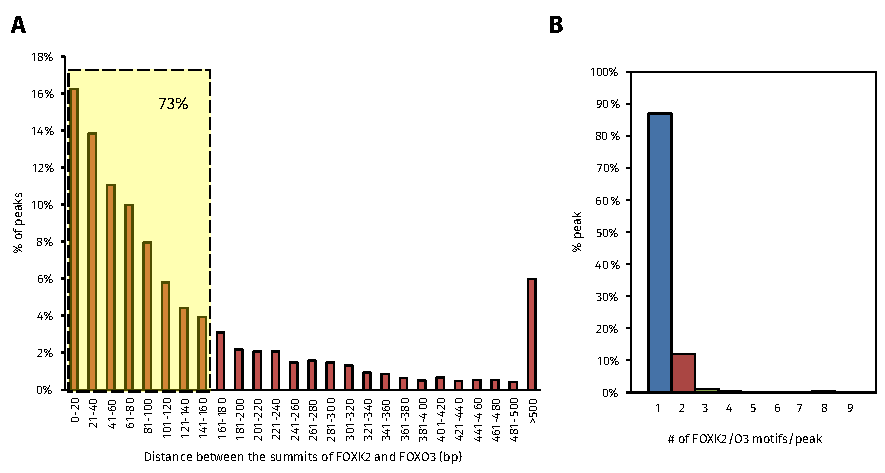
\includegraphics[width=0.9\textwidth]{chapter3/figures_foxo3/fig51.pdf}
    \caption[Distance between FOXK2 and FOXO3 summits and the occurrence of the FOXK2/O3 motifs within the shared peaks]{\textbf{Distance between FOXK2 and FOXO3 summits and the occurrence of the FOXK2/O3 motifs within the shared peaks. (A)} Histogram showing the distance between the FOXK2 and FOXO3 summits. The shared peaks coordinates were extracted, and the distance of the FOXK2 and FOXO3 summits within each peak was calculated. \textbf{(B)} Histogram showing that the frequency of occurrence of FOXK2/O3 motifs (GTAAACA, ATAAACA, GTCAACA and GTAAATA) within the shared peaks. Sequences from the shared peaks ($\pm$ 200 bp from the FOXK2 summits) were extracted, and the occurrence of FOXK2/O3 motifs was counted per peak.}
    \label{fig:fig51}
\end{figure}

In summary, changes of FOXK2 binding do not seem to affect FOXO3 binding, and increased FOXO3 binding cannot displace FOXK2 from the chromatin. Bioinformatic analyses show that the summits of FOXK2 and FOXO3 are very close, and most of their shared peaks only contain one available Forkhead binding site (FOXK2/O3 motifs) per peak, indicating that FOXK2 and FOXO3 are likely to bind to the same site. Therefore, the question still remains: given that FOXK2 and FOXO3 cannot bind to the same site together, what is the relationship between FOXK2 and FOXO3 binding?

\subsection{Summary}

Collectively, the data presented in this section provide a detailed analysis of the FOXO3 ChIP-seq data and a comparison between the FOXO3 and FOXK2 cistromes. Only one experiment was performed for the FOXO3 ChIP-seq, and 6,089 peaks were identified by both MACS and HOMER peak callers.

Many known FOXO3 target genes are successfully detected by our FOXO3 ChIP-seq data. However, a previous study has indicated that FOXO3 binds to the upstream regions of \textit{CCNB1} and \textit{PLK1} promoter, indicating its redundant regulatory role with FOXM1 (\cite{alvarez2001forkhead}). Our FOXO3 ChIP-seq data does not recover such binding events, and ChIP-qPCR results demonstrate that FOXO3 does not bind the core promoters of \textit{CCNB1} and \textit{PLK1} either (\textbf{Figure \ref{fig:fig40}A}). The discrepancy could be due to different experimental conditions: G2-arrested HeLa cells (\cite{alvarez2001forkhead}) and LY294002 treated U2OS cells (this study). A later study has shown that FOXO3 fails to activate a \textit{PLK1} promoter-driven luciferase and forced overexpression of FOXO3 fails to rescue the mitotic defects caused by the loss of FOXM1 (\cite{laoukili2005foxm1}). Therefore, whether FOXO3 really contributes to the execution of mitotic programmes still need further investigation.

Gene ontology analyses recover many known FOXO3 functions like apoptosis, cell cycle arrest, cell differentiation and development. Interestingly, the apoptosis and cell cycle arrest related processes are not enriched when all FOXO3 peaks are analysed. Instead, they are more enriched in the peaks with high FOXO3 binding signals, indicating that high occupancy FOXO3 binding events might reflect the regulation of apoptosis and cell cycle arrest. Novel functions like the regulation of smooth muscle cell migration and blood coagulation are revealed by the FOXO3 ChIP-seq data, suggesting FOXO3 may function as an important regulator within those processes. However, biological functions revealed by our FOXO3 ChIP-seq data must be interpreted with caution, because only one experiment of FOXO3 ChIP-seq was done. Extracting biological functions from a single experiment can be unreliable. In addition, it is interesting to see the differentiation- and development-related terms as well as terms like blood coagulation enriched within the FOXO3 cistrome, considering the U2OS cell line is derived from an osteosarcoma. It is possible that FOXO3 binds to those genes but does not regulate their expression in this cell type. Without downstream experimental validations, no reliable conclusions about the biological functions of FOXO3 can be drawn.

FOXO3 and FOXK2 have both shared and specific peaks, but the majority of FOXO3 binding events are shared with FOXK2. The most overrepresented DNA motifs returned from FOXK2 or FOXO3 ChIP-seq derived peaks are both Forkhead like responsive elements containing the core GTAAACA. Certain substitutions within the core sequence are tolerable, and the consensus can be summarised as RTMAAYA, with GTAAACA being the most frequent motif in both cases. FOXK2 and FOXO3 possess the same sequence preference within the core consensus, but some nucleotides flanking the core consensus are more overrepresented within the FOXK2 peaks, compared to the FOXO3 peaks and the genome background. This preference of FOXK2 towards the flanking nucleotides can be summarised as an extended motif WWGTAAACAWS, and the \textit{in vitro} competition EMSA experiments suggest that mutations of the nucleotides flanking the Forkhead consensus indeed affect the DNA binding of FOXK2. Of note, only nucleotides flanking the most frequent heptameric sequence GTAAACA were investigated in this study. It is possible that when bound to a different core consensus (\textit{e.g.} GTCAACA), FOXK2 or FOXO3 has different preferences at the flanking region. Further experiments need to be done to address this issue.

Besides the Forkhead like motif, several responsive elements that are recognised by other transcription factors are also enriched within the FOXK2 and FOXO3 ChIP-seq derived peaks, and comparisons with other transcription factor ChIP-seq datasets indicate FOXK2 and FOXO3 might cooperate with those transcription factors to regulate gene expression. The CTCF and the ETS1-distal motifs were differentially enriched within the FOXK2 and FOXO3 cistromes respectively. Co-localisation of the binding events between the insulator CTCF and FOXK2, and between ETS1 and FOXO3 were observed, suggesting that CTCF might contribute to FOXK2 specific binding events, and ETS1 might help FOXO3 gain its own specific binding peaks. The different TF-TF cooperation might also help FOXK2 and FOXO3 gain their specific biological functions. However, since the ChIP-seq data sets are from different labs and different cell lines, the comparison performed in this section is just a reference. Without further wet lab experimental validation, no firm conclusions can be drawn.

On the other hand, preliminary data suggests that some cooperation of binding events might exist. For example, our recent study of FOXK2 has revealed many FOXK2 binding proteins including SIN3A and SET (Z.Ji, unpublished data), both of which have been shown to interact with CTCF (\cite{lutz2000transcriptional,yusufzai2004ctcf}). In addition, another CTCF interaction partner YY1 can form a ternary complex with BAP1 and HCF1 (\cite{yu2010the}), both of which interact with FOXK2 (Z.Ji unpublished data). Interestingly, another Forkhead transcription factor FOXA1 is shown to have a subset of binding events that overlap with CTCF (\cite{ross-innes2011a}).

The distance of FOXK2 and FOXO3 summits is close, and the majority of the shared peaks only contain one FOXK2/O3 motif. Since no evidence suggests the FOXK2 physically interacts with FOXO3, hence it is reasonable to speculate that the binding of FOXK2 and FOXO3 at their shared peaks are mutually exclusive (\textit{i.e.} binding at different cells). However, ChIP results indicate that the change of FOXK2 binding does not have any detectable effects on FOXO3 binding within their shared peaks and vice versa. This leaves an interesting question of how they bind to their shared peaks. These two proteins might utilise some novel mechanisms to achieve their binding events at the shared peaks. Further investigation need to be done to address this question (see \textbf{Chapter \ref{ch:conclusions}}).

\chapter{General discussion} \label{ch:discussion}

\section{ChIP-seq methodology}

With the efforts to optimise the ChIP technique and the development of the NGS technology, ChIP-seq offers a robust and powerful way of studying TF-DNA interactions \textit{in vivo}. It is foreseeable that in future, a ChIP-seq experiment will become cheaper and faster. However, there are also many limitations and biases, both experimentally and bioinformatically, for this method. Therefore, when drawing conclusions based on the ChIP-seq data, one must be aware of the potential problems involved in this technique.

\subsection{Experimental limitations} \label{section:chiplimitation}

The quality of the antibody is the primary limitation of the ChIP-seq experiment. During the immunoprecipitation step, both specific and non-specific proteins will be pulled down, and stringent washes (high concentration of salt) are applied later on. Therefore, an ideal antibody should have high specificity so that less non-specific protein is immunoprecipitated, and high affinity so that stringent washes will not disrupt the antibody-antigen binding. However, such antibodies are not always available. Even if an ideal antibody exists, the epitope recognised by the antibody might be masked or destroyed during the crosslinking step. In our case, we have tested several antibodies for FOXM1 and FOXO3 respectively. The FOXM1 antibody from Santa Cruz Technology (C-20, sc-502) works best in our hands, in terms of specificity, sensitivity and IP efficiency. However, in our hands, none of the tested antibodies for FOXO3 are suitable for the ChIP application (Cell Signalling \#9467, Cell Signalling \#2497, Millipore 07-702, and Abcam ab12162).

When no antibody for ChIP is available, the epitope-tagged version of protein of interest can be used. There are a number of choices for the tags in ChIP-seq experiments: FLAG, Myc, V5, GFP, biotin, all of which have been successfully used in ChIP-seq analyses. We have tested both FLAG (N-terminal) and V5 (C-terminal) tags for FOXO3. V5-tagged FOXO3 cannot be efficiently immunoprecipitated by the antibody after crosslinking (data not shown), while the FLAG tag works well for the ChIP of FOXO3. Therefore, a FLAG- tagged FOXO3 stable cell line was generated and used for the ChIP-seq study of FOXO3. When the epitope-tagged version of a protein is used for ChIP-seq, it is generally preferred to have the expression level of the exogenous protein comparable to the endogenous one, \textit{i.e.} not to overexpress, because the overexpression might artificially cause the protein to bind many other places than the endogenous protein. However, this assumption has never been rigorously tested. According to a very recent study which investigated the genome-wide binding events of Olig2 in mouse embryonic stem cells, the binding profiles (number of binding sites, locations of binding sites \textit{etc.}) between the endogenous Olig2 and overexpressed (more than 5 fold) V5-tagged Olig2 are very similar (\cite{mazzoni2011embryonic}). Therefore, whether overexpression can cause artificial binding events still needs to be thoroughly investigated.

Another potential problem of ChIP-seq is regional bias. Usually, during the library preparation step, only small fragments that are within the optimal size range for the NGS application are selected (100 - 200 bp for SOLiD, 300 - 500 bp for Illumina). However, many regions in the genome, like heterochromatin, are highly compacted and therefore are difficult to sonicate. Therefore, those regions that are refractory to sonication tend to be under-represented in ChIP-seq analyses (\cite{teytelman2009impact}). In contrast, regions within open chromatin are generally easier to shear, which often yields higher coverage during the sequencing (\cite{auerbach2009mapping}). Hence, the chromatin state will bias the downstream data analysis.

GC-bias is another issue of ChIP-seq experiments. Since GC-rich sequences are difficult to amplify by the PCR reaction, some high GC-content sequences might be lost during early library preparation steps (\cite{aird2011analyzing}). However, for some unknown reasons, GC-rich sequences tend to be over-represented during the sequencing step on the Illumina platform, which will influence the downstream peak finding steps (\cite{dohm2008substantial,cheung2011systematic}). On the other hand, the SOLiD platform seems to have difficulty recovering GC-rich sequence during the run (see more details in the \textbf{Appendix}). Therefore, when analysing factors, like zinc finger proteins which bind to GC-rich sequences, the data should be treated with caution. Recently, some methods, both experimental and bioinformatical, have been developed for the Illumina platform to reduce these biases (\cite{aird2011analyzing,cheung2011systematic}), and these methods might be useful in future applications.

In addition, sequencing depth is also an important factor when doing ChIP-seq experiments. Intuitively, one criterion to determine whether sufficient sequencing depth has been reached is that no further binding sites can be detected with additional reads (\enquote{saturation point}). However, different transcription factors and peak calling algorithms have various saturation profiles (reviewed in \cite{park2009chip-seq:}). With the advancement of sequencing technology, recent ChIP-seq data sets often contain 10 - 30 M reads per factor in the human genome. Lately, a study suggests such a level of sequencing depth might not be enough for some transcription factors and histone marks (\cite{chen2012systematic}). However, this
suggestion is based on experiments performed in \textit{Drosophila} S2 cells (\cite{chen2012systematic}). Our FOXM1 ChIP-seq experiments yielded 27,892,797 and 8,906,067 uniquely mapped reads for the first and second replicate respectively, and more than 99\% of the reads are not in the FOXM1 binding peaks, indicating that the majority of the mapped reads are actually background, which is a common phenomenon in ChIP-seq analyses (reviewed in \cite{pepke2009computation}). Although it has lower sequencing depth, the second replicate has recovered most FOXM1 binding sites and exhibits relatively higher signals than the first replicate (\textbf{Figure \ref{fig:fig12}}). Therefore, at least in the FOXM1 case, it seems that the current standard sequencing depth (10 - 30 million reads) is enough.

\subsection{Bioinformatical limitations}

After the sequencing, intensive bioinformatic analyses need to be done to extract biological meaning (enriched regions in the case of ChIP-seq) from the huge amount of short sequencing tags.

The first daunting task is mapping the short sequencing reads to reference genomes. Since the sequence of the human genome is not random, highly repeated and degenerated regions are difficult to map. Many computational algorithms are available for mapping, including the most commonly-used ones: MAQ (\url{http://maq.sourceforge.net/}), BOWTIE (h\url{ttp://bowtie-bio.sourceforge.net/index.shtml}), and BFAST (\url{http://bfast.sourceforge.net/}), as well as programs provided by the sequencing companies: ELAND (Illumina) and Corona-Lite (SOLiD). During the reads alignment, a certain extent of mismatch (usually up to 2 mismatches) should be allowed due to sequencing errors, SNPs, and indels or differences between the interrogated genome and the reference genome (reviewed in \cite{park2009chip-seq:}). One of the main issues of mapping is the way of dealing with reads that can be aligned to multiple regions of the genome. Usually, those reads are discarded, and only reads that are uniquely mapped to the genome are preserved. The mapping algorithms also provide the options to retain the reads that can be mapped to multiple positions of genome, given that one position is mapped better than the others. Whether to only keep uniquely mapped reads or not will slightly affect the downstream identification of binding events. We have tried both methods in our FOXM1 and FOXO3 ChIP-seq data sets, and found out that the overall binding patterns and conclusions are not affected (data not shown).

Another bioinformatically challenging task for ChIP-seq is the peak calling. After the alignment of reads, one needs to identify statistically significant enriched regions, \textit{i.e.} binding events. Dozens of peak calling algorithms are available. In general, there are two major types of peak calling methods: sliding window based method (\textit{e.g.} MACS) and kernel density estimation based method (\textit{e.g.} QuEST). The former divides the genome into small overlapping or non-overlapping windows and calculates the number of reads and statistical significance within each window based on certain probability models (\textit{e.g.} Poisson and binomial distributions); the latter is a non-parametric (\textit{i.e.} does not rely on any distributions) method to facilitate finding the aggregation of densely packed short sequencing reads which leads to the identification of binding events. Direct comparisons of many peak callers were performed recently (\cite{wilbanks2010evaluation,feng2011peakranger:}). Although certain peak callers seem to outperform others, due to poorly defined standards in some cases, no conclusive remarks can be drawn from the comparisons (\cite{wilbanks2010evaluation}). In our study, MACS and HOMER are used for the peak calling, because: 1) MACS is widely used and has been shown to be good at detecting both punctate and broad peaks; 2) HOMER is a multi-functional software suite which is user- friendly and easy for wet lab biologists to use, and it also has been demonstrated to be robust for analysing both transcription factor and histone modification ChIP-seq data (\cite{heinz2010simple,lin2010a,wang2011reprogramming}).

Despite the lack of benchmarks for the data analysis, high confidence binding events are always revealed no matter what method is used. Some specific binding/regulatory events at certain loci will be affected by the computational methods used. For example, in our FOXK2 and FOXO3 ChIP-seq data, MACS and HOMER revealed similar numbers of binding events respectively, but only 50 \textasciitilde 60\% of the binding sites were called by both algorithms. However, the overall conclusions from a ChIP-seq experiment will not be affected by the method used. This can be demonstrated by the fact that most ChIP-seq results conducted in different labs and using different methods are still very consistent with known biological functions and biochemical properties of the factor of interest. Therefore, by performing biological replicates or using various analytical tools, the data extracted from ChIP-seq experiments can be very robust (\cite{wilbanks2010evaluation}).

\section{Genome-wide TF-DNA binding events}

The interaction between DNA and transcription factors is the fundamental basis for generating transcriptional networks. The specific structures and amino acids within the DNA-binding domains mean that transcription factors can only bind to certain DNA sequences. However, the \textit{in vivo} DNA-binding events of transcription factors are determined by more than the simple protein-DNA recognition.

\subsection{Only a small proportion of consensus binding sites are occupied by a factor}

The first complicated scenario is that not all potential binding sites are actually occupied by a transcription factor. Given a certain cell type at a certain condition, a transcription factor seems to only select a subset of available consensus sequences to bind. The GTAAACA sequence occurs 472,221 times in the human genome according to the unmasked hg18 assembly. In terms of sequence, there should be 472,221 available binding sites for any given Forkhead transcription factor. Considering the degenerate nature of TF-DNA binding, this number is still an underestimation. However, only 1.6\% and 0.34\% of the GTAAACA sequences are occupied by FOXK2 and FOXO3 respectively. Similar observations are also seen for many other transcription factors (reviewed in \cite{pan2010mechanisms}). It seems this is a general phenomenon related to the \textit{in vivo} DNA-binding events of transcription factors.

It has been suggested that nucleosomes are the barriers that block a transcription factor binding to its consensus sequence (reviewed in \cite{li2007the}). Therefore, one reason that the majority of consensus sequences are not bound by the transcription factors could be that they are compacted within nucleosomes. However, some proteins like Forkhead transcription factors can act like pioneer factors which are able to bind to condensed chromatin (reviewed in \cite{zaret2011pioneer}). Hence, the nucleosome occupancy only partially explains why a consensus site is not bound by a factor. In addition, DNA methylation within the consensus sequences may also contribute to the DNA binding of a transcription factor. For example, the methylation of the CpG within the CTCF consensus motif blocks its binding (\cite{bell2000methylation}), while ZBTB33 (also known as Kaiso) only binds to methylated GC-rich sequences (\cite{yoon2003n-cor}). However, there are no CpGs within the Forkhead consensus, and this is not likely to be relevant here.

Another mechanism that controls transcription factor selectivity is the cooperative binding with other proteins. Since transcription factors are thought to never work alone, they always bind to \textit{cis}-regulatory modules which are often occupied by a number of transcription factors at the same time (reviewed in \cite{farnham2009insights}). Therefore, the binding of a transcription factor is often affected by the binding of other transcription factors. Indeed, when comparing the genome-wide binding events of FOXM1, FOXO3 and FOXK2 to the ChIP-seq of many other transcription factors from the ENCODE project, the binding sites of FOXM1, FOXO3 and FOXK2 are usually associated with other transcription factor DNA-binding events, although there are no apparent connections among them (\textbf{Figure \ref{fig:fig52}}, note the overlap between grey bars and coloured bars). In general, a transcription factor is more likely to bind to the regions where there are other transcription factor binding events nearby.

\begin{figure}[!h]
    \centering
    \includegraphics[width=0.9\textwidth]{chapter4/figures/fig52.pdf}
    \caption[Examples of the overlapping of binding events for FOXM1, FOXO3, FOXK2 and other transcription factors from the ENCODE project]{\textbf{Examples of the overlapping of binding events for FOXM1, FOXO3, FOXK2 and other transcription factors from the ENCODE project.} Genomic binding profiles of FOXM1, FOXO3 and FOXK2 from a region of chromosome 1 or chromosome 12. The binding events of FOXM1 (red), FOXO3 (orange) and FOXK2 (blue) are shown as coloured bars below their binding profiles. The binding sites of all other available transcription factors are shown in grey bars at the bottom. This data is taken from the ENCODE project which contains more than 20 transcription factor ChIP-seq data sets in 25 different cell types. The intensity of the grey bar indicates the number of transcription factors bound in that region. Note the overlap between coloured bars and grey bars.}
    \label{fig:fig52}
\end{figure}

\subsection{Not all binding events involve the consensus motifs}

Another common phenomenon in the transcription factor ChIP-seq data is that not all binding events contain the consensus motif of the protein of interest. In the FOXK2 and FOXO3 binding regions, only \textasciitilde 25\% of them contain the strong motif GTAAACA. When taking the weaker motif (RTMAAYA) into account, there are still \textasciitilde 40\% binding events that do not contain a consensus motif. Since formaldehyde can crosslink both protein-DNA and protein-protein interaction during the ChIP experiments, a protein can be indirectly linked to the DNA by interacting with other DNA-binding factors. In fact, in the FOXK2 and FOXO3 cistromes, motifs bound by other transcription factors (\textit{e.g.} AP1, CTCF and ETS1) occur more frequently within the peaks which do not contain the RTMAAYA motif (data not shown). Therefore, the differential enrichment of different motifs and the overlapping with various transcription factors within FOXK2 and FOXO3 binding regions suggest that some indirect DNA contact exist in these two factors. This indirect recruitment is a universal mechanism used by many other transcription factors to bind to chromatin \textit{in vivo} (reviewed in \cite{farnham2009insights}).

FOXM1 seems to be an extreme example where its consensus motif is not enriched within its binding regions at all. A previous study indicates that FOXM1 has very low affinity ($\mu$M) to the Forkhead consensus sequence, presumably due to the lack of sugar-phosphate backbone contacts with the DNA (\cite{littler2010structure}). In the crystal structure of the DNA-binding domains of Forkhead transcription factors, the third $\alpha$-helix ($\alpha$3) reaches into the major groove of the DNA, making sequence-specific contacts with the DNA via hydrogen bonds and van-der-Waals interactions (\textbf{Figure \ref{fig:fig53}}, yellow arrows). In other Forkhead transcription factors like FOXA, FOXK, and FOXO, the second \enquote{wing} (W2) which consists of positively charged amino acids also interacts with the DNA at the sugar- phosphate backbone, the minor groove and the major groove (\textbf{Figure \ref{fig:fig53}}, white arrows). In stark contrast, the W2 of FOXM1 adopts a unique structure which diverges away from the DNA (\textbf{Figure \ref{fig:fig53}}, the rightmost panel, the white arrow). The lack of W2-DNA interaction might be the reason that FOXM1 possesses such a low affinity to the Forkhead consensus (\cite{littler2010structure}). Interestingly, a recent study has solved the crystal structure of ASH2L and revealed that it also holds a Forkhead-like winged-helix domain. The affinity of ASH2L to its consensus sequence is also very low ($\mu$M), presumably due to its negatively charged W2 which cannot stably interact with the DNA (\cite{sarvan2011crystal}).

\begin{figure}[!h]
    \centering
    \includegraphics[width=\textwidth]{chapter4/figures/fig53.pdf}
    \caption[Comparisons of crystal structures of the DNA-binding domains of FOXA3, FOXK2, FOXO3 and FOXM1 in a complex with Forkhead consensus DNA sequence]{\textbf{Comparisons of crystal structures of the DNA-binding domains of FOXA3, FOXK2, FOXO3 and FOXM1 in a complex with Forkhead consensus DNA sequence.} Pictures are taken from the Protein Data Bank. The $\alpha$3 and the W2 of each DNA-binding domain are indicated by the yellow and white arrows respectively.}
    \label{fig:fig53}
\end{figure}

It is possible that such a low affinity to DNA might yield the small number of binding sites for FOXM1. Considering there are multiple Forkhead proteins present within the cell, it is reasonable to speculate that FOXM1 is unable to compete with other Forkhead proteins, such as FOXK2 and FOXO3, to bind the canonical Forkhead consensus. Therefore, the Forkhead consensus is not enriched in the FOXM1 cistrome. This is, indeed, supported by our ChIP-seq studies.

\section{Genome-wide DNA-binding events among family members}

Since members within the same family can bind to the same consensus sequence, and often multiple members from the same family are expressed in a cell, the binding events among family members can be very complicated.

First, the number of binding sites varies greatly within individual members. The difference of the number of binding sites among Forkhead proteins is a good example (\textbf{Table \ref{table:fkhtfschip}}). The Forkhead DNA-binding domain has been shown to structurally resemble linker histone (\cite{clark1993co-crystal}), indicating that the Forkhead transcription factors can stably interact with DNA. Consistent with this notion, certain Forkhead transcription factors, like FOXA1 and FOXI1, have been proven to be able to bind condensed chromatin (\cite{cirillo1998binding,yan2006the}). Therefore, one often expects Forkhead transcription factors have many binding sites. Indeed, many Forkhead transcription factors, like FOXA1, FOXP3 together with our FOXK2 and FOXO3, do meet that expectation. However, some Forkhead transcription factors, like FOXP2 and FOXM1, have relatively fewer binding sites than others (\textbf{Table \ref{table:fkhtfschip}}). This difference can be partially derived from the endogenous protein levels, the cellular conditions, the cell lines and the antibodies used in the experiments. In addition, the small number of binding sites of FOXM1 and its extreme low affinity to the DNA imply that protein-DNA affinity might also contribute to the number of binding sites in vivo, and our FOXM1 ChIP-seq studies support this idea.

Second, family members often have both redundant and specific binding events despite the fact that they all bind to the same sequence \textit{in vitro}. It has been suggested that nucleotides within and flanking the core sequence can influence the binding of individual members. In this study, although no discernible preferences can be detected within the Forkhead consensus between FOXK2 and FOXO3, the nucleotides flanking the core consensus contribute to the DNA binding of FOXK2 both \textit{in vivo} and \textit{in vitro}. Similar observations are also seen within members from the ETS-domain transcription factor family (\cite{wei2010genome-wide}). In addition, a recent PBM study suggests that besides the consensus motif (primary site) recognised by a transcription factor, most proteins can also bind to multiple distinct DNA motifs (secondary, tertiary sites \textit{etc.}) (\cite{badis2009diversity}). In some cases, the binding of a transcription factor to the secondary site is equally efficient as to the primary site (\cite{badis2009diversity}). Many transcription factors from the same family have very similar primary site, but the differences among their secondary sites can be quite different (\cite{badis2009diversity}). For example, among all five tested mouse Forkhead transcription factors, the primary sites for them are Forkhead-like consensus containing GTAAACA, but the secondary sites are relatively more variable: TAACA for Foxa2, AYAACA for Foxj1 and Foxk1, CAHAACA for Foxj3 (\textbf{Figure \ref{fig:fig54}}). Therefore, it is tempting to speculate that the differences of the secondary sites of FOXK2 and FOXO3 might also contribute to their \textit{in vivo} DNA binding. Unfortunately, such data is not available yet.

\begin{figure}[!h]
    \centering
    \includegraphics[width=0.9\textwidth]{chapter4/figures/fig54.pdf}
    \caption[Comparison of the primary and the secondary binding sites of five mouse Forkhead transcription factors]{\textbf{Comparison of the primary and the secondary binding sites of five mouse Forkhead transcription factors.} The PBM data of five indicated mouse Forkhead transcription factors are from the Uniprobe database (\cite{Newburger2009-uc}).}
    \label{fig:fig54}
\end{figure}

Another conundrum is the binding relationship of family members within their redundant binding events. When only one site is available within the redundant binding region, the binding of family members to the binding site is generally thought to be mutually exclusive. Therefore, one often expects competition between family members on the same site, unless they can form a complex. Indeed, competition of the binding between family members has been observed \textit{in vitro}, in yeast and in human (\cite{pierce2003sum1,boros2009overlapping,zhou2011integrated,lickwar2012genome-wide}). However, in this study, we failed to identify any relationship between the binding of FOXK2 and FOXO3 at their shared peaks, since changes in FOXK2 ChIP signals do not affect the FOXO3 ChIP signals and vice versa. The relationship of binding among family members on the same site might be more than just simple competition. Indeed, a recent study using a modified ER (ER pBox) which possesses the same binding specificity as GR demonstrates that these two proteins fail to exhibit any competition even though they are thought to bind exactly the same site (\cite{voss2011dynamic}). Therefore, similar to the ER pBox and GR, one possible explanation for this is that the binding between FOXK2 and FOXO3 to the DNA is quite dynamic, that is, the residence time for the proteins at the DNA is very short. In this case, the available binding site is never really saturated, leading to a consequence that multiple family members can bind to the exact the same site without competing with one another. This is in contrast to a long-residence time binding situation where the available binding site is occupied by one family member for a relatively long time (saturated), and this binding can be competed by other family members when the concentrations of proteins are changed (\textbf{Figure \ref{fig:fig55}}).

\begin{figure}[!h]
    \centering
    \includegraphics[width=0.9\textwidth]{chapter4/figures/fig55.pdf}
    \caption[Two possible models of TF-DNA occupancy \textit{in vivo}]{\textbf{Two possible models of TF-DNA occupancy \textit{in vivo}. Top,} long-residence time binding. Members within the transcription factor family \textbf{$X$} can bind to their consensus Motif \textbf{$X$}. Long-residence time binding (black lines) of a family member (\textbf{$X_a$} or \textbf{$X_b$}) makes the Motif \textbf{$X$} saturated which is less accessible (dotted lines) to other family members (\textbf{$X_a$} or \textbf{$X_b$}). \textbf{Bottom,} short-residence time binding. Members bind to the Motif \textbf{$X$} in a \enquote{hit-and-run} manner, and the Motif \textbf{$X$} is always available for the binding regardless of the concentrations of family members.}
    \label{fig:fig55}
\end{figure}

\chapter{Conclusions} \label{ch:conclusions}

\section{Summary of findings}

Transcription factor-DNA interactions \textit{in vivo} are the fundamental events in the regulatory network of transcription. The interrogation of genome-wide binding events of three Forkhead transcription factors presented in this study demonstrates that the DNA binding of a transcription factor in a living cell involves great subtleties.

FOXM1 does not bind to the canonical Forkhead consensus \textit{in vivo}, although specific interactions between FOXM1 and the Forkhead consensus can be observed \textit{in vitro} at a low affinity. Instead, the chromatin recruitment of FOXM1 needs the presence of the MMB complex. It cooperates with the MMB complex to occupy the promoters of a large array of genes whose transcriptional activities peak at the G2 and M phases. Therefore, FOXM1 gains its own specific binding events and unique functions in the regulation of the mitosis relative to other Forkhead proteins by interacting with the MMB complex. These findings reinforce the notion that the protein-protein interaction plays an essential role in the achievement of specific binding events of a transcription factor \textit{in vivo}.

FOXK2 and FOXO3 bind to both specific and shared regions in the genome, and the majority of the FOXO3 binding events are shared with FOXK2. Both factors bind to the Forkhead consensus \textit{in vitro} and \textit{in vivo}, but sequence preferences at the positions flanking the Forkhead consensus partially dictate the specific binding sites of FOXK2, which strengthens previous findings that nucleotides flanking the core consensus are important for the specificity among family members (\cite{wei2010genome-wide}). Furthermore, different TF-TF interactions also possibly contribute to the specific binding events of FOXK2 and FOXO3. In addition, neither competitive nor assisted binding can be observed between the binding of FOXK2 and FOXO3 on their shared binding regions, indicating that their binding at those regions might be highly dynamic.

Based on the results presented in this study, we propose the following models for the \textit{in vivo} DNA-binding events of FOXM1, FOXK2 and FOXO3: under normal condition when PI3K/AKT pathway is active, FOXO3 is sequestered in the cytoplasm; FOXM1 and FOXK2 are in the nucleus, but FOXM1 is unable to compete with FOXK2 to bind the Forkhead consensus; instead, FOXM1 occupies the promoters where the CHR motif is located by interacting with the MMB complex, and this MMB/FOXM1 complex plays a critical role in the transcriptional regulations of the genes whose activities peak at the G2 and M phases (\textbf{Figure \ref{fig:fig56}}, top panel); when the PI3K/AKT pathway is inhibited, FOXO3 enters into the nucleus and mostly binds to regions where FOXK2 is located, but the relationship between the binding of FOXK2 and FOXO3 remains unknown (\textbf{Figure \ref{fig:fig56}}, bottom panel).

\begin{figure}[!h]
    \centering
    \includegraphics[width=0.9\textwidth]{chapter5/figures/fig56.pdf}
    \caption[Models for the DNA-binding events of FOXM1, FOXK2 and FOXO3 \textit{in vivo}]{\textbf{Models for the DNA-binding events of FOXM1, FOXK2 and FOXO3 \textit{in vivo}.} See the main text for detailed description. The dotted line represents the nuclear envelope.}
    \label{fig:fig56}
\end{figure}

\section{Unanswered questions and future work}

\subsection{Does FOXM1 directly contact DNA \textit{in vivo}?}

Since formaldehyde can crosslink both protein-DNA and protein-protein interactions, a binding event of a transcription factor detected by ChIP experiments can be due to both direct and indirect DNA contacts. It is impossible to tell whether a protein really directly contacts DNA using ChIP experiments. However, if a consensus motif is present around the summit of a transcription factor binding site, one tends to believe that it is a direct contact. Unfortunately, this is not the case in the FOXM1 cistrome. We do notice that some FOXM1 binding events do not overlap with either LIN9 or B-MYB, indicating that some chromatin binding events of FOXM1 are probably independent of the MMB complex. Therefore, it is still possible that FOXM1 directly contact DNA or is recruited by another factor. Motif discovery is supposed to shed some light on this, but this analysis only returns the CCAAT-box motif, the CHR motif and a GC-rich motif. It is possible that some zinc-finger proteins, which bind to the GC-rich sequence, recruit FOXM1 to the chromatin of the promoters at a subset of its target genes, or that FOXM1 binds to a very short DNA element which contains little information content that cannot be discovered by motif analysis. Therefore, it is necessary to utilise high resolution ChIP-exo (\cite{rhee2011comprehensive}) to reveal the exact crosslinking point of FOXM1 or the proteins recruiting FOXM1 to the chromatin, which might help elucidate how FOXM1 is recruited to the chromatin.

\subsection{What is the intrinsic DNA binding specificity of FOXK2 and FOXO3?}

ChIP-seq analyses of FOXK2 and FOXO3 demonstrate that both factors can bind to the Forkhead consensus. There are no discernible preferences within the core consensus, but FOXK2 favours the sequence WWGTAAACAWS. However, the sequence motif returned by the ChIP-seq data is biased by the non-random nature of the genome, and it does not reflect the intrinsic specificity of a factor. Although bandshift experiments suggest that the nucleotides flanking the Forkhead consensus do affect the binding of FOXK2, this method is only at a low-throughput level. Therefore, to systematically investigate the intrinsic DNA binding specificity of FOXK2 and FOXO3, in vitro methods such as PBM or HT- SELEX can be used. The comparison between results from ChIP-seq and PBM/HT- SELEX of FOXK2 and FOXO3 could be very informative.

\subsection{What is the relationship of the DNA binding between FOXK2 and FOXO3 at their shared binding regions?}

Since the change of FOXK2 binding does not affect the binding of FOXO3 at the shared binding regions and vice versa, it is difficult to draw a conclusion about the relationship between DNA binding of FOXK2 and FOXO3. So far, all the experiments are done within 24 - 48 hours after the depletion of FOXK2 or the overexpression of FOXO3. It is possible that this time frame is too soon to see any effect, and that longer depletion or overexpression might help to uncover the relationship of the binding between these two factors. However, current ChIP experiments detect the steady-state binding of a factor across a population of cells. FOXK2 and FOXO3 might occupy the same locus but in different cells, and the general occupancy detected by ChIP is only a fraction of the cells. If the model proposed in \textbf{Figure \ref{fig:fig55}} is true, current ChIP technique will never catch such dynamic changes of binding. Therefore, other methods based on fluorescent microscopy like FRET or FRAP which can study protein-DNA interaction in a single cell might help to elucidate this question, but this will not allow the investigation at a single gene locus level. In addition, it is still possible that FOXK2 and FOXO3 bind to different sites within the shared peaks, which cannot be discriminated by the current resolution of sonication-based ChIP-seq. Therefore, it is necessary to perform ChIP-reChIP experiments to investigate whether FOXK2 and FOXO3 co-associate on chromatin in the same cell. High resolution ChIP-exo will also help to reveal the exact binding sites of FOXK2 and FOXO3.

\subsection{How are the binding events of FOXO3 linked to its biological functions?}

Linking the binding events of a transcription factor to its functions is critical for understanding the biological meanings of transcription factor-DNA interactions \textit{in vivo}. Extracting biological meanings from only one experiment can be dangerous, considering the dynamic nature of the TF-DNA interactions \textit{in vivo}. Therefore, in order to investigate the functions of the FOXO3 binding events, a repeat of FOXO3 ChIP-seq experiment needs to be done. Furthermore, to understand how functional specificity is achieved by FOXK2 and FOXO3, it is necessary to use gene expression arrays to find out the FOXO3-regulated genes, and make comparisons to the FOXK2-regulated genes (\cite{ji2012the}).

\appendix
\chapter[Appendix]{Appendix} \label{ch:appendix}

Due to unknown technical issues, it seems that the SOLiD sequencer has some problems recovering the CpG islands from the genome. We experienced repeated failure of performing FOXM1 ChIP-seq experiments using the SOLiD platform. The problems do not seem to be the library preparation, since good fold enrichments on target genes can be detected both before and after the library preparation (\textbf{Figure \ref{fig:fig57}A}). By using the Illumina platform, FOXM1 ChIP-seq experiments were successfully done without any problems.

When comparing the binding profiles of the FOXM1 ChIP-seq experiments from SOLiD and Illumina, SOLiD fails to recover all the 270 peaks which are detected by both Illumina platform and ChIP-qPCR (\textbf{Figure \ref{fig:fig57}B}).

\begin{figure}[!h]
    \centering
    \includegraphics[width=0.9\textwidth]{appendix/figures/fig57.pdf}
    \caption[Examples of technical issues of the SOLiD platform]{\textbf{Examples of technical issues of the SOLiD platform. (A)} ChIP-qPCR on the indicated FOXM1 target genes before (left) and after (right) the library preparation for the SOLiD platform. Fold enrichments over the \textit{PLK1} negative region are shown. \textbf{(B) Left,} an example of the Illumina profile (top) and the SOLiD profile (bottom) at the \textit{FZR1} locus. \textbf{Right,} heatmap of tag density profiles of FOXM1 ChIP-seq tags from the Illumina and the SOLiD platforms around the 270 peaks of FOXM1. Tags were calculated in every 50 bp bin, and the density profiles were normalised to tags per 10 million total reads per bin. The middle point of each panel (indicated by small arrows below) represents the summit of the FOXM1 peak generated using the Illumina platform. 5 kb upstream and 5 kb downstream around the summit were plotted. \textbf{(C)} Quantification of average tags around the transcription start sties (TSS) of all RefSeq genes. Genes were aligned by their TSS, and the region of -1000 and +1000 bp relative to the TSS was selected. Tags were calculated in every 10 bp bin and normalised to tags per 10 million total reads per bin per gene. \textbf{(D)} The same analysis as \textbf{(C)} but using the reads from the indicated ChIP samples and different sequencing platforms.}
    \label{fig:fig57}
\end{figure}

When aligning the reads from input samples to the transcription start sites of all Refseq annotated genes, which ideally should be uniformly distributed, the input sample from the Illumina platform has a slight enrichment around the TSS (\textbf{Figure \ref{fig:fig57}C}, the blue line), which is a common phenomenon in ChIP-seq studies (\cite{auerbach2009mapping,cheung2011systematic}), presumably because many TSS regions are located within open chromatin regions which tend to get higher coverage (see \textbf{Section \ref{section:chiplimitation}}). Surprisingly, the input sample from the SOLiD platform from our core facility exhibits a \enquote{dip} in tag density around the TSS regions (\textbf{Figure \ref{fig:fig57}C}, the grey line). This is not a specific issue from this study, because an input sample of MCF10A cells from another experiment (\cite{odrowaz2012elk1}) also shows a similar depletion of reads around the TSS regions (\textbf{Figure \ref{fig:fig57}C}, the orange line). This is not a specific issue from our core facility either, because our FOXK2 ChIP- seq data was done at a facility from Life Technology, and the input sample from the FOXK2 ChIP-seq data also exhibits a \enquote{dip} in tag density around the TSS regions (\textbf{Figure \ref{fig:fig57}C}, the black line).

When aligning the reads from FOXM1 ChIP samples to the transcription start sites, the sample from the Illumina platform exhibits a nice enrichment in tag density around the TSS regions of all Refseq annotated genes (\textbf{Figure \ref{fig:fig57}D}, the red line), which is consistent with its experimental validation. In contrast, the sample from the SOLiD platform, again, shows a \enquote{dip} in tag density around the TSS regions (\textbf{Figure \ref{fig:fig57}D}, the grey line). This seems to be a specific problem for FOXM1, because FOXK2 and ELK1 (both from the SOLiD platform) show good enrichments surrounding the TSS regions (\textbf{Figure \ref{fig:fig57}D}, the blue and the black lines). Interestingly, FOXO3 ChIP signals (SOLiD platform) also displays a depletion of reads near the TSS regions (\textbf{Figure \ref{fig:fig57}D}, the orange line).

It seems that the SOLiD platform is able to detect some binding events near promoters as demonstrated by ELK1 which also tends to bind promoter regions (\cite{odrowaz2012elk1}). We next noticed that 77\% FOXM1 binding events overlap with the CpG islands, while 46\% ELK1 binding sites are within the CpG islands, and only 2.5\% and 10.3\% FOXK2 and FOXO3 peaks overlap with the CpG islands respectively. Therefore, we suspect that the SOLiD platform may have problems recovering the CpG islands from the genome.

Since the FOXM1 ChIP-seq experiments failed in the SOLiD platform, the comparisons between different sequencing platforms using the FOXM1 data might not be appropriate. To gain a preliminary idea about the potential differences between the Illumina and SOLiD sequencing platforms, we used our FOXK2 ChIP-seq data which were performed on both the SOLiD and the Illumina platforms at the same time, and both platforms successfully identified similar numbers of FOXK2 binding peaks.

\begin{figure}[!h]
    \centering
    \includegraphics[width=0.9\textwidth]{appendix/figures/fig58.pdf}
    \caption[Comparisons between the FOXK2 ChIP-seq data from the Illumina and the SOLiD platforms]{\textbf{Comparisons between the FOXK2 ChIP-seq data from the Illumina and the SOLiD platforms. (A)} Percentages of peaks distributions identified from different platforms. The genome background is also shown. The promoter region was defined as 5'- UTR and up to 1000 bp upstream from the TSS. \textbf{(B)} Quantification of average tags from the Illumina platform (the red line) and the SOLiD platform (the black line) around the TSS of all RefSeq genes (left) and the CpG islands (right). Genes were aligned by their TSS and the CpG islands were aligned by their mid point. The region of -1000 and +1000 bp relative to the TSS or the centre of the CpG islands was selected. Tags were calculated in every 10 bp bin and normalised to tags per 10 million total reads per bin per region. \textbf{(C)} The same analysis as \textbf{(B)} but only using the reads from the SOLiD sequencing platforms.}
    \label{fig:fig58}
\end{figure}

First, we checked the genomic distributions of FOXK2 peaks identified from the SOLiD and the Illumina platforms respectively. Higher percentage of peaks from the Illumina platform were located in the promoter regions (\textbf{Figure \ref{fig:fig58}A}), while the distributions of peaks at other locations were relatively similar (data not shown). When compared to the overlap with CpG islands, the difference between the peaks from the two platforms was even more prominent (\textbf{Figure \ref{fig:fig58}A}). Next, we checked the FOXK2 ChIP signals around either the TSS regions or the CpG islands. The signals from the Illumina platform were much higher than those from the SOLiD platform in both cases (\textbf{Figure \ref{fig:fig58}B}), indicating SOLiD platform has a problem recovering the signals from these regions. When looked into the detail of the ChIP signals from the SOLiD platform, FOXK2 still showed a slight enrichment around the TSS regions (\textbf{Figure \ref{fig:fig58}C}, left panel), but there was a \enquote{dip} in tag density of FOXK2 around the CpG islands (\textbf{Figure \ref{fig:fig58}C}, right panel). Therefore, we suspect that the SOLiD platform may have problems recovering the CpG islands from the genome.

Considering the limitations of the SOLiD platform, the overlap between FOXK2, FOXO3 and FOXM1 presented in this study might be an underestimation. The binding of FOXK2 and FOXO3 to the promoter regions might be underestimated as well. However, since direct comparisons between FOXK2 and FOXO3 are performed within the same platform, we argue that the overall conclusions should not be greatly affected.

%\bibliographystyle{plain}
%\bibliography{PhD_thesis}

\setstretch{1}
\setlength\bibitemsep{4pt}
\printbibliography[title={Reference},heading=bibintoc]

\end{document}